% This one will format for two-sided binding (ie left and right pages have mirror margins; blank pages inserted where needed):
%\documentclass[a4paper,twoside]{ociamthesis}
% This one will format for one-sided binding (ie left margin > right margin; no extra blank pages):
%\documentclass[a4paper]{ociamthesis}
% This one will format for PDF output (ie equal margins, no extra blank pages):
\documentclass[a4paper,nobind]{ociamthesis} 

% !TEX root = ../main.tex

%%%%% SELECT YOUR DRAFT OPTIONS
% Three options going on here; use in any combination.  But remember to turn the first two off before
% generating a PDF to send to the printer!
% This highlights (in blue) corrections marked with (for words) \mccorrect{blah} or (for whole
% paragraphs) \begin{mccorrection} . . . \end{mccorrection}.  This can be useful for sending a PDF of
% your corrected thesis to your examiners for review.  Turn it off, and the blue disappears.
\correctionstrue

%%%%% BIBLIOGRAPHY SETUP
\usepackage{natbib}
\bibliographystyle{plainnat}
% This makes the bibliography left-aligned (not 'justified') and slightly smaller font.
\renewcommand*{\bibfont}{\small}

%%%%% THESIS / TITLE PAGE INFORMATION
% Everybody needs to complete the following:
\title{Automating Inference, Learning, and Design}
\author{Tom Rainforth}
\college{Wolfson College}

% Your full degree name.  (But remember that DPhils aren't "in" anything.  They're just DPhils.)
\degree{Doctor of Philosophy}
% Term and year of submission, or date if your board requires (eg most masters)
\degreedate{Trinity 2017}

\usepackage{microtype}

% use Times
\usepackage{times}
% For figures
\usepackage{graphicx} % more modern
%\usepackage{epsfig} % less modern
%\usepackage{subfigure} 
\usepackage{subcaption} 
\graphicspath{{./part/ipmcmc/figures/}{./misc/figures/}{./bopp/figures/}{./opt/figures/}{./design/figures/}{./nest/figures/}{./inf/figures/}{./part/figures/}{./bayes/figures/}}
\usepackage{tikz}
\usetikzlibrary{fit}					% fitting shapes to coordinates
\usetikzlibrary{backgrounds}	% drawing the background after the foreground
\usepackage{setspace}

\usepackage{cancel}

%\usepackage{svg}

% For algorithms


% For math
\usepackage{amsthm}
\usepackage{dsfont}
\usepackage{amssymb,amsmath}
\usepackage{bbm}

%\newcommand{\theHalgorithm}{\arabic{algorithm}}

\usepackage{hyperref}

\usepackage{bibentry}
\nobibliography*


% % BOPP

%\usepackage{enumitem}
%\setlist[itemize]{leftmargin=*}
%\usepackage{paralist}
\usepackage{footmisc}
\usepackage{listings}
\usepackage{color}
\usepackage{xcolor}
\usepackage{textcomp}
\usepackage{xspace}
\usepackage{amsbsy}
\usepackage{siunitx}
%\usepackage{algorithmicx}
%\usepackage{algpseudocode}
\usepackage{mathtools}
\usepackage{array}
\usepackage{booktabs}
\usepackage{adjustbox}
\usepackage{microtype}
\usepackage{todonotes}

\usepackage{wrapfig}
\usepackage{thmtools}
\usepackage{thm-restate}

\newcommand{\angurl}{\scriptsize \url{http://www.robots.ox.ac.uk/~fwood/anglican}}
\newcommand{\myurl}{\scriptsize \url{https://bitbucket.org/twgr/ipmcmc}}

%\definecolor{darkgreen}{rgb}{0.25,.5,0}
%\definecolor{blue}{rgb}{0,0.33,0.66}
%\definecolor{red}{rgb}{0.66,0.0,0.0}
%\definecolor{purple}{rgb}{0.33,0,0.66}
%\definecolor{cyan}{rgb}{0.0,0.5,0.5}
%\definecolor{orange}{rgb}{0.5,0.25,0.0}
%\definecolor{gray}{rgb}{0.4,0.4,0.4}
\lstset{ 
	language=Lisp, 
	basicstyle=\small\ttfamily,
	keywordstyle={}, 
	alsoletter={/},
	alsoletter={:},
	alsoletter={*},
	alsoletter={<-},
	commentstyle=\em \color{gray}, 
	frame=lines,
	%float=tbph,
	% captionpos=b,
	showstringspaces=false, 
	keywordstyle=[1]\bf\ttfamily\color{blue},
	keywords=[1]{BO,theta-best,bo-acquire,sample-initial-points,sample,observe,observe*,observe<-,predict,store,retrieve,return,catch,throw},
	keywordstyle=[2]\bf\ttfamily\color{red},
	keywords=[2]{defn,if,let,letfn,loop,looppredict,recur},
	keywordstyle=[3]\bf\ttfamily\color{cyan},
	keywords=[3]{absorb,assoc,argmax,count,cons,conj,dirichlet-discrete,do,exponential,first,flip,fn,gamma,beta,get,keys,lazy-seq,map,mvn-niw,nth,mat/add,mat/div,normal,print,produce,reduce,repeat,repeatedly,rest,set,shape,take,uniform-continuous,vec,distribution,factor,simulate,abc-likelihood,when,max},
	keywordstyle=[4]\bf\ttfamily\color{purple},
	keywords=[4]{defopt,defquery,doopt,doquery,query,defdist},
	keywordstyle=[5]\ttfamily\color{orange},
	keywords=[5]{:nu,:alpha,:id},
	mathescape=true,
	stringstyle={},
} 
\lstnewenvironment{code}[2]{\lstset{caption=#1,label=#2}}{}

\newtheorem{example}{Example} 
\newtheorem{theorem}{Theorem}[chapter]
\newtheorem{lemma}[theorem]{Lemma} 
%\newtheorem{proposition}[proposition]{Proposition} 
\newtheorem{remark}{Remark}
%\newtheorem{corollary}[corollary]{Corollary}
\newtheorem{definition}{Definition}[chapter]
%\newtheorem{conjecture}[conjecture]{Conjecture}
%\newtheorem{axiom}[axiom]{Axiom}

% % % % % % % % % % % % % % % % % % %


\usepackage{packages/naesseth}
%\usepackage{packages/algorithm,packages/algorithmic}
\usepackage{packages/abbreviations}

\usepackage{algorithmicx}
\usepackage{algorithm}
\usepackage{algpseudocode}
\usepackage{setspace}
% % % % % % % % %
\algnewcommand\algorithmicswitch{\textbf{switch}}
\algnewcommand\algorithmiccase{\textbf{case}}
\algnewcommand\algorithmicassert{\texttt{assert}}
\algnewcommand\Assert[1]{\State \algorithmicassert(#1)}%
% New "environments"
\algdef{SE}[SWITCH]{Switch}{EndSwitch}[1]{\algorithmicswitch\ #1\ \algorithmicdo}{\algorithmicend\ \algorithmicswitch}%
\algdef{SE}[CASE]{Case}{EndCase}[1]{\algorithmiccase\ #1}{\algorithmicend\ \algorithmiccase}%
%\algtext*{EndSwitch}%
\algtext*{EndCase}%

%\ShortHeadings{Automating Inference, Learning, and Design}{Tom Rainforth}
%\firstpageno{1}

\begin{document} 

%%%%% CHOOSE YOUR LINE SPACING HERE
% This is the official option.  Use it for your submission copy and library copy:
\setlength{\textbaselineskip}{22pt plus2pt}
% This is closer spacing (about 1.5-spaced) that you might prefer for your personal copies:
%\setlength{\textbaselineskip}{18pt plus2pt minus1pt}

% You can set the spacing here for the roman-numbered pages (acknowledgements, table of contents, etc.)
\setlength{\frontmatterbaselineskip}{17pt plus1pt minus1pt}

% Leave this line alone; it gets things started for the real document.
\setlength{\baselineskip}{\textbaselineskip}


%%%%% CHOOSE YOUR SECTION NUMBERING DEPTH HERE
% You have two choices.  First, how far down are sections numbered?  (Below that, they're named but
% don't get numbers.)  Second, what level of section appears in the table of contents?  These don't have
% to match: you can have numbered sections that don't show up in the ToC, or unnumbered sections that
% do.  Throughout, 0 = chapter; 1 = section; 2 = subsection; 3 = subsubsection, 4 = paragraph...

% The level that gets a number:
\setcounter{secnumdepth}{2}
% The level that shows up in the ToC:
\setcounter{tocdepth}{2}

% JEM: Pages are roman numbered from here, though page numbers are invisible until ToC.  This is in
% keeping with most typesetting conventions.
\begin{romanpages}
	
	% Title page is created here
	\maketitle
	
	%%%%% DEDICATION -- If you'd like one, un-comment the following.
	%\begin{dedication}
	%This thesis is dedicated to\\
	%someone\\
	%for some special reason\\
	%\end{dedication}
	
	%%%%% ACKNOWLEDGEMENTS -- Nothing to do here except comment out if you don't want it.
	\begin{acknowledgements}
		% !TEX root = ../main.tex

\vspace{20pt}
I would first like to thank by partner Sophie for her support and understanding through this
process and for all the sacrifices she has made on my behalf.  I would similarly like to
thank my family for their unwavering support and making me who I am today.  I would like
to thank Frank Wood, Jan-Willem van de Meent, and Brooks Paige for their guidance and
support, both academic and personal.  I owe them all, particularly Frank and Jan-Willem,
a huge debt of gratitude for teaching me most of what I know, nurturing me from an
arrogant fool who asked questions like \emph{Metropolis what?} to an even more arrogant
fool who thinks he knows everything.  This work would have been a terrible failure without them.
I would like to thank my friends and colleagues 
Atılım Güneş Baydin, Rob Cornish, Piotr Czaban, Neil Dhir, Jack Fitzsimons, Adam Goliński,
Bradley Gram-Hansen, Max Igl, David Janz, Tom Jin, Tuan Anh Le, Mario Lezcano, 
Aravindh Mahendran, David Martínez Rubio, Siddharth N, Nantas Nardelli, Michael Osborne,
Nick Palmius, Yura Perov, David Tolpin, Andrea Vedaldi, Andrew Warrington, Stefan Webb, 
Hongseok Yang, Yuan Zhou, and Rob Zinkov, for making this time in Oxford some of the 
happiest of my life.  I would like to thank my previously unmentioned coauthors Arnaud Doucet, Fredrik Lindsten,
Christian A. Naesseth, and Benjamin Vincent, for being an absolute pleasure to work with.
Finally, I would like to thank BP for providing the funding for this research.

Much of the novel material in this thesis is from coauthored work and it would be fabrication
to claim it all as my own.  In particular, a lot of the work is based around the probabilistic 
programming system \emph{Anglican}, for which all the credit must go to Frank Wood,
Jan-Willem van de Meent, and David Tolpin. Elsewhere, citations are made
to the original coauthored papers upon which this work is based, for which credit
must go to all my coauthors.
	\end{acknowledgements}
	
	%%%%% ABSTRACT -- Nothing to do here except comment out if you don't want it.
	\begin{abstract}
		% !TEX root = ../main.tex

\vspace{20pt}
Imagine a world where computational simulations can be inverted as easily as running them forwards, where data
can be used to refine models automatically, and where the only expertise one needs to carry
out powerful statistical analysis is a basic proficiency in scientific coding.  Creating such a
world is the ambitious long-term aim of \emph{probabilistic programming}.

The bottleneck for improving the probabilistic models, or simulators, used throughout the quantitative sciences,
is often not an ability to devise better models conceptually,  but a lack of expertise,
time, or resources to realize such innovations.
Probabilistic programming systems (PPSs) help alleviate this bottleneck 
by providing an expressive and accessible modeling framework,
%, often more in line we conventional scientific simulation than mainstream statistical approaches,
 then
automating the required computation to draw inferences from the model, for example finding
the model parameters likely to give rise to a certain output.
By decoupling model specification and inference, PPSs 
streamline the process of developing and drawing inferences from new models, while
opening up powerful statistical methods to non-experts.
%open up powerful statistical methods 
%to non-experts, while
%streamlining the process of developing new models or inference algorithms
%those within the machine learning and statistics communities.  
Many systems further provide
the flexibility to write new and exciting models which would be hard, or even impossible, to convey using 
conventional statistical frameworks.

The central goal of this thesis is to improve and extend PPSs.
%, providing some of the many steps
%that will be necessary to achieve the lofty long-term aims of the field.  
In particular, we will
make advancements to the underlying inference engines and increase the
range of problems which can be tackled.  For example, we will extend PPSs to a mixed inference-optimization
framework, thereby providing automation of tasks
such as model learning and engineering design.  Meanwhile, we make inroads into constructing systems
for automating adaptive sequential design problems, providing potential applications across the sciences.
Furthermore, the contributions of the work reach far beyond probabilistic programming, as 
achieving our goal will require us to make
advancements in a number of related fields such as particle Markov chain Monte Carlo methods,
Bayesian optimization, and Monte Carlo fundamentals. %, and Bayesian experimental design.

%
%Specifically, we will introduce \emph{interacting particle
%	Markov chain Monte Carlo},
%a new inference algorithm suitable for large-scale computation, and 
%detail is implementation as a general purpose inference engine for the PPS \emph{Anglican}. 
%%explain how it can be
%%used as general purpose inference engine for PPSs by detailing its implementation
%%in the PPS \emph{Anglican}.  
%We will extend PPSs beyond their typical inference setting
%to a more general mixed inference-optimization framework by introducing~\emph{Bayesian
%	optimization for probabilistic programs}, thereby providing automation of tasks
%such as model learning and engineering design.
%%in the same manner as inference is automated in existing systems.  
%We will develop theoretical 
%results on \emph{nesting Monte Carlo
%	estimators} and explain the important implications these have for nesting models in PPSs.
%Finally, we will 
%%examine a particular
%%class of nested estimation problems, those of Bayesian experimental design, and 
%introduce a high-level framework for automating adaptive sequential design problems, 
%%a particle example 
%providing application of our technique to psychological trials.
%%Finally, we will examine a particular
%%class of nested estimation problems, those of Bayesian experimental design, and introduce
%%a high-level framework for automating arbitrary adaptive sequential design problems,
%%providing application our technique to psychological trials.
	\end{abstract}
	
	%%%%% MINI TABLES
	% This lays the groundwork for per-chapter, mini tables of contents.  Comment the following line
	% (and remove \minitoc from the chapter files) if you don't want this.  Un-comment either of the
	% next two lines if you want a per-chapter list of figures or tables.
	\dominitoc % include a mini table of contents
	%\dominilof  % include a mini list of figures
	%\dominilot  % include a mini list of tables
	
	% This aligns the bottom of the text of each page.  It generally makes things look better.
	\flushbottom
	
	% This is where the whole-document ToC appears:
	\tableofcontents
	
	%\listoffigures
	\mtcaddchapter
	% \mtcaddchapter is needed when adding a non-chapter (but chapter-like) entity to avoid confusing minitoc
	
	% Uncomment to generate a list of tables:
	%\listoftables
	%	\mtcaddchapter
	
	%%%%% LIST OF ABBREVIATIONS
	% This example includes a list of abbreviations.  Look at text/abbreviations.tex to see how that file is
	% formatted.  The template can handle any kind of list though, so this might be a good place for a
	% glossary, etc.
	% !TEX root = ../main.tex

% First parameter can be changed eg to "Glossary" or something.
% Second parameter is the max length of bold terms.
\begin{mclistof}{Glossary and Abbreviations}{3.2cm}

\item[\smc] Sequential Monte Carlo.  A general purpose inference method using a series of 
intermediary targets.

\end{mclistof} 

	
	% The Roman pages, like the Roman Empire, must come to its inevitable close.
\end{romanpages}

% !TEX root = ../main.tex

\begin{savequote}[8cm]
	\textlatin{Le doute n'est pas une état bien agréable, mais l'assurance est un état ridicule.}
	
	Doubt is not a very agreeable status, but certainty is a ridiculous one.
	\qauthor{--- Voltaire}
\end{savequote}

\chapter{Introduction}
\label{sec:intro}

This is Chapter~\ref{sec:intro}.

% !TEX root = ../main.tex

\chapter{Interacting Particle Markov Chain Monte Carlo}
\label{sec:ipmcmc}

% !TEX root = ../main.tex

% Intro, contribution statement and related work
\section{Introduction}
\label{sec:ipmcmc:intro}
%In this paper we propose the interacting particle Markov chain Monte Carlo (\ipmcmc), a particle Markov chain Monte Carlo (\pmcmc) method that is suitable to execution on distributed and multi-core computing architectures and present empirical results suggesting significant improved mixing rates relative to both non-interacting \pg nodes and a single \pg node with an identical computational budget. 

In this section we introduce \emph{interacting particle Markov chain Monte Carlo} (\ipmcmc), a \pmcmc method based on an interacting pool of standard and conditional sequential Monte Carlo samplers. Like related methods, \ipmcmc is a Markov chain Monte Carlo sampler on an extended space. We present empirical results that show significant improvements in mixing rates relative to both non-interacting \pmcmc samplers, and a single \pmcmc sampler with an equivalent memory and computational budget. 
An additional advantage of the \ipmcmc method is that it is suitable for distributed and multi-core architectures.  

%In this paper we present a Markov chain Monte Carlo (\mcmc) method that employs a pool of particle Markov chain Monte Carlo (\pmcmc) and sequential Monte Carlo (\smc) samplers. 
\mcmc methods are a fundamental tool for generating samples from a posterior density in Bayesian data analysis (see \eg, \citet{robert2013monte}). Particle Markov chain Monte Carlo (\pmcmc) methods, introduced by \citet{andrieuDH2010}, make use of sequential Monte Carlo (\smc) algorithms \citep{gordon1993novel,doucet2001sequential} to construct efficient proposals for the \mcmc sampler. 

One particularly widely used \pmcmc algorithm is particle Gibbs (\pg). The \pg algorithm modifies the \smc step in the \pmcmc algorithm to sample the latent variables conditioned on an existing particle trajectory, resulting in what is called a conditional sequential Monte Carlo (\csmc) step. The \pg method was first introduced as an efficient Gibbs sampler for latent variable models with static parameters \citep{andrieuDH2010}. Since then, the \pg algorithm and the extension by \citet{lindstenJS2014} have found numerous applications in \eg Bayesian non-parametrics \citep{ValeraFSPC2015,tripuraneni2015}, probabilistic programming \citep{wood2014new,vandemeent_aistats_2015} and graphical models \citep{everitt2012,naessethLS2014,naessethLS2015nested}.  

A drawback of PG is that it can be particularly adversely affected by \emph{path degeneracy} in the CSMC step.  Conditioning on an existing trajectory means that whenever resampling of the trajectories results in a common ancestor, this ancestor must correspond to this trajectory.  Consequently, the mixing of the Markov chain for the early steps in the state sequence can become very slow when the particle set typically coalesces to a single ancestor during the CSMC sweep.

In this paper we propose the interacting particle Markov chain Monte Carlo (\ipmcmc) sampler. In \ipmcmc we run a pool of \csmc and unconditional \smc algorithms as parallel processes that we refer to as nodes. After each run of this pool, we apply successive Gibbs updates to the indexes of the \csmc nodes, such that the indices of the \csmc nodes changes. Hence, the nodes from which retained particles are sampled can change from one MCMC iteration to the next. This lets us trade off exploration (\smc) and exploitation (\csmc) to achieve improved mixing of the Markov chains. Crucially, the pool provides numerous candidate indices at each Gibbs update, giving a significantly higher probability that an entirely new retained particle will be ``switched in'' than in non-interacting alternatives.

This interaction requires only minimal communication; each node must report an estimate of the marginal likelihood and receive a new role (\smc or \csmc) for the next sweep. This means that \ipmcmc is embarrassingly parallel and can be run in a distributed manner on multiple computers.

%We introduce the interacting particle Markov chain Monte Carlo (\ipmcmc) method, a new type of 
%high-dimensional \tom{The phrase high-dimensional seems a little out of place here to me.  I understand what you are saying but it is maybe a bit premature to make the point}
%Monte Carlo integration method enabling efficient 

We prove that \ipmcmc is a partially collapsed Gibbs sampler on the extended space containing the particle sets for all nodes. In the special case where \ipmcmc uses only \emph{one} \csmc node, it can in fact be seen as a non-trivial and unstudied instance of the $\alpha$-\smc-based \citep{whiteley2016} \pmcmc method introduced by \citet{huggins2015}. However, with \ipmcmc we extend this further to allow for an arbitrary number of \csmc and standard \smc algorithms with interaction. Our experimental evaluation shows that \ipmcmc outperforms both independent \pg samplers as well as a single \pg sampler with the same number of particles run longer to give a matching computational budget.

An implementation of iPMCMC is provided in the probabilistic programming system \emph{Anglican}\footnote{\angurl} \citep{wood2014new}, whilst illustrative MATLAB code, similar to that used for the experiments, is also provided\footnote{\myurl}.

%Our key contribution is the \ipmcmc method, %with a highly efficient off-the-shelf \brooks{what do you mean by ``off the shelf''?} \mcmc method, the interacting particle Markov chain Monte Carlo (\ipmcmc), that also can make systematic use of distributed or multi-core computing architectures. 

%\tom{Should we maybe add the longer run chains to results to that we can make this point clearly?}
%\fredrik{Is the last sentence ok?}
% !TEX root = ../main.tex

\section{Background}
\label{sec:ipmcmc:background}
We start by briefly reviewing sequential Monte Carlo \citep{gordon1993novel,doucet2001sequential} and the particle Gibbs algorithm \citep{andrieuDH2010}. Let us consider a non-Markovian latent variable model of the following form
\begin{subequations}
	\label{eq:ssm}
	\begin{alignat}{2}
	x_t | x_{1:t-1} &\sim f_t(x_t | x_{1:t-1}), \\
	y_t | x_{1:t} &\sim g_t(y_t|x_{1:t}),
	\end{alignat}
\end{subequations}
where $x_t \in \setX$ is the latent variable and $y_t \in \setY$ the observation at time step $t$, respectively,
with transition densities $f_t$ and observation densities $g_t$; $x_1$ is drawn from some initial distribution $\mu(\cdot)$. The method we propose is not restricted to the above model, it can in fact be applied to an arbitrary sequence of targets.

%We focus on the non-Markovian latent variable model because it has been shown to be useful within \eg probabilistic programming \citep{wood2014new}.%However, we restrict the exposition to the latent variable model for clarity and to see the potential usefulness of it to \eg probabilistic programming \citep{wood2014new}. \tom{I am not sure I agree with this statement - PP should actually allow the most general possible use of iPMCMC.  I think we would be better making the point that its ability to operate on arbitrary models make it a suitable candidate for PP inference engines.  By the final draft I would expect us to have it running and publically availible in Anglican}

We are interested in calculating expectations with respect to the posterior distribution $p(x_{1:T}|y_{1:T})$ on latent variables $x_{1:T} \eqdef (x_1,\ldots,x_T)$ conditioned on observations $y_{1:T} \eqdef (y_1,\ldots,y_T)$, which is proportional to the joint distribution $p(x_{1:T}, y_{1:T})$,
\begin{align}
\label{eq:jointdistribution}
p(x_{1:T} | y_{1:T}) \propto  \mu(x_1) \prod_{t=2}^T f_t(x_t | x_{1:t-1}) \prod_{t=1}^T g_t(y_t|x_{1:t}).\nonumber
\end{align}
In general, computing the posterior $p(x_{1:T}|y_{1:T})$ is intractable and we have to resort to approximations. We will in this paper focus on, and extend, the family of particle Markov chain Monte Carlo algorithms originally proposed by \citet{andrieuDH2010}. The key idea in \pmcmc is to use \smc to construct efficient proposals of the latent variables $x_{1:T}$ for an \mcmc sampler.

%
%   SMC
%

\begin{algorithm}[tb]
	\caption{Sequential Monte Carlo \hfill {\small (all for $i=1,\ldots,N$)}}
	\label{alg:smc}
	\begin{spacing}{1.2}
	\begin{algorithmic}[1]
		\STATE {\bfseries Input:} data $y_{1:T}$, number of particles $N$, proposals $q_t$
		\STATE $x_1^i \sim q_1(x_1)$
		\STATE $w_1^i = \frac{g_1(y_1|x_1^i) \mu(x_1^i)}{q_1(x_1^i)}$
		\FOR{$t = 2$ {\bfseries to} $T$}
		\STATE $a_{t-1}^i \sim \Discrete\left(\left\{\nw_{t-1}^{\ell}\right\}_{\ell=1}^N\right)$% \tom{We can maybe more general that categorical here?}
		\STATE $x_t^i \sim q_t(x_t | x_{1:t-1}^{a_{t-1}^i})$ 
		\STATE Set $x_{1:t}^i = (x_{1:t-1}^{a_{t-1}^i},x_t^i)$
		\STATE $w_t^i = \frac{g_t(y_t|x_{1:t}^i) f_t(x_t^i | x_{1:t-1}^{a_{t-1}^i})}{q_t(x_t^i|x_{1:t-1}^{a_{t-1}^i})}$
		\ENDFOR
	\end{algorithmic}
\end{spacing}
\end{algorithm}

\subsection{Sequential Monte Carlo}
\label{sec:ipmcmc:background:smc}
The \smc method is a widely used technique for approximating a sequence of target distributions: in our case $p(x_{1:t}|y_{1:t}) = p(y_{1:t})^{-1} p(x_{1:t},y_{1:t}), ~t=1,\ldots,T$. 
At each time step $t$ we 
%assume we have access to 
generate a \emph{particle system}
$\{(x_{1:t}^i,w_{t}^i)\}_{i=1}^N$ which provides a weighted approximation  to $p(x_{1:t}|y_{1:t})$. Given such a weighted particle system at time $t-1$, this 
%The particle system is then
is propagated forward in time to $t$ by first drawing an ancestor variable $a_{t-1}^i$ for each particle from its corresponding distribution:
\begin{align}
\Prb(a_{t-1}^i = \ell) &= \nw_{t-1}^\ell.
&
\ell&=1,\ldots,N,
\end{align}
where $\nw_{t-1}^\ell = w_{t-1}^\ell / \sum_i w_{t-1}^i$. This is commonly known as the resampling step in the literature. We introduce the ancestor variables $\{a_{t-1}^i\}_{i=1}^N$ explicitly to simplify the exposition of the theoretical justification given in Section \ref{sec:theory}.

We continue by simulating from some given proposal density $x_t^i \sim q_t(x_t | x_{1:t-1}^{a_{t-1}^i})$ and re-weight the system of particles as follows:
\begin{align}
\label{eq:smcweights}
w_t^i = \frac{g_t(y_t|x_{1:t}^i) f_t(x_t^i | x_{1:t-1}^{a_{t-1}^i})}{q_t(x_t^i|x_{1:t-1}^{a_{t-1}^i})},
\end{align}
where $x_{1:t}^i = (x_{1:t-1}^{a_{t-1}^i},x_t^i)$. This results in a new particle system $\{(x_{1:t}^i,w_t^i)\}_{i=1}^N$ that approximates $p(x_{1:t}|y_{1:t})$. A summary is given in Algorithm~\ref{alg:smc}.

%Let $q_{\text{SMC}}(\xb^{1:N},\ab^{1:N})$ denote the joint probability distribution over $\xb^{1:N}=x_{1:T}^{1:N}, \ab^{1:N} = a_{1:t-1}^{1:N}$ induced by running Algorithm~\ref{alg:smc}. We can write the complete distribution, which will be useful for the correctness proof, as follows
%\begin{align}
%q_{\text{SMC}}(\xb^{1:N},\ab^{1:N}) = \prod_{i=1}^N q_1(x_1^i) \prod_{t=2}^T \frac{W_{t-1}^{a_{t-1}^i}}{\sum_\ell W_{t-1}^\ell} q_t(x_t^i|x_{1:t-1}^{a_{t-1}^i}).
%\end{align}

% 
%   PG
% 
\subsection{Particle Gibbs}
\label{sec:ipmcmc:background:pg}
The \pg algorithm \citep{andrieuDH2010} is a Gibbs sampler on the extended space composed of all random variables generated at one iteration, which still retains the original target distribution as a marginal. Though \pg allows for inference over both latent variables and static parameters, we will in this paper focus on sampling of the former.  The core idea of \pg is to iteratively run \emph{conditional} sequential Monte Carlo (\csmc) sweeps as shown in Algorithm~\ref{alg:csmc}, whereby each conditional trajectory is sampled from the surviving trajectories of the previous sweep.  This \emph{retained particle} index, $b$, is sampled with probability proportional to the final particle weights $\bar{w}^i_T$. 


\begin{algorithm}[tb]
	\caption{Conditional sequential Monte Carlo}
	\label{alg:csmc}
	\begin{spacing}{1.2}
	\begin{algorithmic}[1]
		\STATE {\bfseries Input:} data $y_{1:T}$, number of particles $N$, proposals $q_t$, conditional trajectory $x_{1:T}'$
		\STATE $x_1^i \sim q_1(x_1), ~i=1,\ldots,N-1$ and set $x_1^N = x_1'$
		\STATE $w_1^i = \frac{g_1(y_1|x_1^i) \mu(x_1^i)}{q_1(x_1^i)}, ~i=1,\ldots,N$
		\FOR{$t = 2$ {\bfseries to} $T$}
		\STATE $a_{t-1}^i \sim \Discrete\left(\left\{\nw_{t-1}^\ell\right\}_{\ell=1}^N\right), ~i=1,\ldots,N-1$
		\STATE $x_t^i \sim q_t(x_t | x_{1:t-1}^{a_{t-1}^i}), ~i=1,\ldots,N-1$
		\STATE Set $a_{t-1}^N = N$ and $x_t^N = x_t'$
		\STATE Set $x_{1:t}^i = (x_{1:t-1}^{a_{t-1}^i},x_t^i), ~i=1,\ldots,N$
		\STATE $w_t^i = \frac{g_t(y_t|x_{1:t}^i) f_t(x_t^i | x_{1:t-1}^{a_{t-1}^i})}{q_t(x_t^i|x_{1:t-1}^{a_{t-1}^i})}, ~i=1,\ldots,N$
		\ENDFOR
	\end{algorithmic}
\end{spacing}
\end{algorithm}

%In the same way as above for the standard \smc algorithm we can define a joint probability distribution induced by running Algorithm~\ref{alg:csmc} %$q_{\text{CSMC}}(\xb^{1:N},\ab^{1:N}\backslash\{\xb^N,\bb^N\} | \xb^N,\bb^N)$, induced by running Algorithm~\ref{alg:csmc}, where $\xb^N, \bb^N$ is the retained (conditioning) particle. 
%\begin{align}
%&q_{\text{CSMC}}\left(\xb^{1:N},\ab^{1:N} \backslash \{\xb^N, \bb^N\} \mid \xb^N, \bb^N, k \right) = \nonumber \\
%&\prod_{\substack{i=1\\i\neq b_{1}}}^N \left[ q_1(x_{1}^i) \right] \prod_{t=2}^T \prod_{\substack{i=1\\i\neq b_{t}}}^N \left[\frac{W_{t-1}^{a_{t-1}^i}}{\sum_\ell W_{t-1}^\ell} q_t(x_{t}^i|x_{1:t-1}^{a_{t-1}^i})\right],
%\end{align}
%where $\xb^N, \bb^N$ is the retained (conditioning) particle.
%\brooks{doesn't make sense --- if the retained particle is $N$, why is it $\xb_m^k, \bb_m^k$ in the above equation? shouldn't $\xb_m^{1:N},\ab_m^{1:N} \backslash \{\xb_m^k, \bb_m^k\}$ actually be $\xb_m^{1:N-1},\ab_m^{1:N-1}$?}


%
%   Limitations
%
%\subsection{Parallelisation and Limitations}
%\label{sec:limitations}
%Our main goal is to increase the efficiency of particle \mcmc, particle Gibbs especially, by coupling independent \smc methods with \csmc algorithms, perhaps running on different workers or threads. The method we propose, interacting particle Markov chain Monte Carlo (\ipmc), makes efficient use of multi-core and distributed computing architectures to increase accuracy of the Monte Carlo sampler.

%The basic \pg typically suffers from the \emph{path degeneracy} effect of \smc samplers, \ie sample impoverishment due to frequent resampling, which leads to bad mixing of the Markov chain. Since we force one trajectory, the conditional part, to survive to the end it means that for early time steps we will almost always pick the corresponding sample from last iteration. To counteract this we might need a very high number of particles to get good mixing for all latent variables $x_{1:T}$, which can be infeasible due to e.g.~limited available memory. The \ipmc can alleviate this issue by a non-standard coupling of several conditional and unconditional (standard) \smc algorithms. The algorithm lets us, from time to time, completely switch out a \csmc particle system with a completely independent \smc one, resulting in improved mixing of the Markov chain.

% !TEX root = ../main.tex

% Here we describe the proposed method and its theoretical properties
\section{Interacting Particle Markov Chain Monte Carlo}
\label{sec:method}
%Our main goal with the interacting particle Markov chain Monte Carlo method is to increase the efficiency of particle \mcmc, particle Gibbs especially, by coupling independent \smc methods with \csmc algorithms, perhaps running on different nodes or threads. The method we propose, interacting particle Markov chain Monte Carlo (\ipmc), makes efficient use of multi-core and distributed computing architectures to increase accuracy of the Monte Carlo sampler.

The main goal of \ipmcmc is to increase the efficiency of \pmcmc, in particular particle Gibbs. The basic \pg algorithm is especially susceptible to the \emph{path degeneracy} effect of \smc samplers, \ie sample impoverishment due to frequent resampling.  Whenever the ancestral lineage collapses at the early stages of the state sequence, the common ancestor is, by construction, guaranteed to be equal to the retained particle.  This results in high correlation between the samples, and poor mixing of the Markov chain. %Since we force one trajectory, the conditional part, to survive to the end it means that for early time steps we will almost always pick the corresponding sample from last iteration. 
To counteract this we might need a very high number of particles to get good mixing for all latent variables $x_{1:T}$, which can be infeasible due to e.g.~limited available memory. \ipmc can alleviate this issue by, from time to time, switching out a \csmc particle system with a completely independent \smc one, resulting in improved mixing.

\ipmcmc, summarized in Algorithm~\ref{alg:ipmc}, consists of $M$ interacting separate \csmc and \smc algorithms, exchanging only very limited information at each iteration to draw new \mcmc samples. We will refer to these internal \csmc and \smc algorithms as nodes, and assign an index $m=1,\ldots,M$. 
At every iteration, we have $P$ nodes running local \csmc algorithms, with the remaining
$M-P$ nodes running independent \smc.
The \csmc nodes are given an identifier $c_j \in \{1,\ldots,M\}, ~j=1,\ldots,P$ with $c_j \neq c_k,~k \neq j$ and we write $c_{1:P} = \{c_1,\ldots,c_P\}$. Let $\xb_m^i = x_{1:T,m}^i$ be the internal particle trajectories of node $m$.

\begin{algorithm}[tb]
	\caption{\ipmcmc sampler}
	\label{alg:ipmc}
	\begin{spacing}{1.2}
	\begin{algorithmic}[1]
		\renewcommand{\algorithmicrequire}{\textbf{Inputs:}}
		\renewcommand{\algorithmicensure}{\textbf{Outputs:}}				 
		\Require number of nodes $M$, conditional nodes $P$ and \mcmc steps $R$, initial $\xb_{1:P}'[0]$
		\For{$r = 1$ {\bfseries to} $R$}
		\State Workers $1:M \backslash c_{1:P}$ run Algorithm~\ref{alg:smc} (\smc)
		\State Workers $c_{1:P}$ run Algorithm~\ref{alg:csmc} (\csmc), conditional on $\xb_{1:P}'[r-1]$ respectively.
		\For{$j = 1$ {\bfseries to} $P$}
		\State Select a new conditional node by simulating $c_j$ according to \eqref{eq:simConditional}. %with probability 
		\State Set new \mcmc sample $\xb_j'[r] = \xb_{c_j}^{b_j}$ by simulating $b_j$ according to~\eqref{eq:simTrajectory}
		\EndFor
		\EndFor
	\end{algorithmic}
\end{spacing}
\end{algorithm}

Suppose we have access to $P$ trajectories ${\xb_{1:P}'[0]=(\xb_1'[0],\ldots,\xb_P'[0])}$ corresponding to the initial retained particles, where the index $[\cdot]$ denotes \mcmc iteration. At each iteration $r$, the nodes $c_{1:P}$ run \csmc (Algorithm~\ref{alg:csmc}) with the previous \mcmc sample $\xb_j'[r-1]$ as the retained particle. The remaining $M-P$ nodes run standard (unconditional) \smc, \ie Algorithm~\ref{alg:smc}.  Each node $m$ returns an estimate of the marginal likelihood for the internal particle system defined as
\begin{align}
\label{eq:ML}
\hat Z_{m} = \prod_{t=1}^T \frac{1}{N} \sum_{i=1}^N w_{t,m}^{i}.
\end{align}
%along with a single trajectory $\xb_{m}^{s_m}$ sampled according to 
%\begin{align}
%\label{eq:simTrajectory}
%\Prb(s_m = i) &= \nw_{T,m}^i
%\end{align}
%where $s_m$ is the local index of the sampled particle.  

The new conditional nodes are then set using a single loop $j=1:P$ of Gibbs updates, sampling new indices $c_j$ where
\begin{align}
\label{eq:simConditional}
&\Prb(c_j = m|c_{1:P\backslash j}) = \hat\nz_{m}^j \\
\label{eq:zeta_def}
\mathrm{and}  \quad &{\hat\nz_{m}^j = \frac{\hat Z_{m} \iden_{m \notin c_{1:P \backslash j}}}{ \sum_{n=1}^M \hat Z_{n} \iden_{n \notin c_{1:P \backslash j}}}},
%\Prb(c_j = m|c_{1:P\backslash j}) = \frac{\hat Z_{\pi_T,m} \iden_{m \notin c_{1:P \backslash j}}}{\sum_{n=1}^M \hat Z_{\pi_T,n} \iden_{n \notin c_{1:P \backslash j}}},
\end{align}
defining ${c_{1:P\backslash j} = \{c_1,\ldots,c_{j-1},c_{j+1},\ldots,c_P\}}$.  We thus loop once through the conditional node indices and resample them from the union of the current node index and the unconditional node indices\footnote{Unconditional node indices here refers to all $m \notin c_{1:P}$ at that point in the loop. It may thus include nodes who just ran a CSMC sweep, but have been ``switched out'' earlier in the loop.}, in proportion to their marginal likelihood estimates.  This is the key step that lets us switch completely the nodes from which the retained particles are drawn.


%The retained particles are the corresponding trajectories sampled in \eqref{eq:simTrajectory} such that 
%\begin{align}
%\label{eq:setTrajectory}
%\xb_j'[r] &= \xb_{c_j}^{b_j}, \quad \mathrm{where} \quad b_j = s_{c_j}, \quad j=1,\dots,P.
%\end{align}

%This step, by far the most computationally demanding, can be trivially parallelised over the $M$ nodes. However, it need not be parallelised to see convergence benefits and reduced memory footprints compared to competing \pmcmc methods.
%\begin{figure}[h]
%\centering
%\resizebox{.45\textwidth}{!}{
%\tikzstyle{smc}=[circle,
                                    thick,
                                    minimum size=1.2cm,
                                    draw=blue!80,
                                    fill=blue!40]
\tikzstyle{csmc}=[circle,
                                    thick,
                                    minimum size=1.2cm,
                                    draw=red!80,
                                    fill=red!20]

\tikzstyle{background}=[rectangle,
                                                fill=gray!10,
                                                inner sep=0.2cm,
                                                rounded corners=5mm]

\begin{tikzpicture}[>=latex,text height=1.5ex,text depth=0.25ex]
  \matrix[row sep=0.5cm,column sep=0.5cm] {
    %&
        \node (j) []{$m$};           &
        \node (j1) []{$\mathbf{1}$}; &
        \node (j2) []{$\mathbf{2}$}; &
        \node (j3) []{$\mathbf{3}$}; &
        \node (j4) []{$\mathbf{4}$}; &
        \node (j5) []{$\mathbf{5}$}; &
        \\
        &
        \node (d1) []{$\vdots$}; &
        \node (d2) []{$\vdots$}; &
        \node (d3) []{$\vdots$}; &
        \node (d4) []{$\vdots$}; &
        \node (d5) []{$\vdots$}; &
        \\
        \node (r-1) []{$r-1$};      &
        \node (r-1_1) [smc]{};      &
        \node (r-1_2) [smc]{};      &
        \node (r-1_3) [csmc]{};     &
        \node (r-1_4) [smc]{};      &
        \node (r-1_5) [csmc]{};     &
        \\
        \node (r) []{$r$};          &
        \node (r_1) [smc]{};        &
        \node (r_2) [csmc]{};       &
        \node (r_3) [smc]{};        &
        \node (r_4) [smc]{};        &
        \node (r_5) [csmc]{};       &
        \\
        \node (r+1) []{$r+1$};      &
        \node (r+1_1) [smc]{};      &
        \node (r+1_2) [csmc]{};     &
        \node (r+1_3) [smc]{};      &
        \node (r+1_4) [smc]{};      &
        \node (r+1_5) [csmc]{};     &
        \\
        &
        \node (d21) []{$\vdots$}; &
        \node (d22) []{$\vdots$}; &
        \node (d23) []{$\vdots$}; &
        \node (d24) []{$\vdots$}; &
        \node (d25) []{$\vdots$}; &
        \\
    };

    \path[->]
        %(A) edge[thick] (x)	% 

        ;
    \begin{pgfonlayer}{background}
        \node [background,
                    fit=(r-1_1) (r-1_5)] {};
        \node [background,
                    fit=(r+1_1) (r+1_5)] {};
    \end{pgfonlayer}
\end{tikzpicture}

%}
%\caption{A high-level illustration of the \ipmcmc algorithm flow for $M=5$ and $P=2$. \csmc nodes are \emph{red} and \smc nodes are \emph{blue}, which means that for example at iteration $r-1$ we have $c_{1:P} = \{3,5\}$.}\label{fig:algorithm}
%\end{figure}
%\tom{You can't tell the difference between these nodes when printed in black and white so would be good to adjust the colours slightly.  I think the index needs to be m not j?  Also might be nice to have something in caption like here we have have $c_{1:P}[r-1] = {1,2}$ here just allow the figure to be a reference to the notation.} 

%The next step involves exchange of information--we need access to the normalisation constant estimates from each node to sample the next \mcmc output $\xb_j'[r]$. The normalisation constant estimate for each node $m$ is computed using the internal particle system as ${\hat Z_{m} = \prod_{t=1}^T \frac{1}{N} \sum_{i=1}^N w_{t,m}^{i}}$.
%%\begin{align}
%%\hat Z_{\pi_T,m} = \prod_{t=1}^T \frac{1}{N} \sum_{i=1}^N w_{t,m}^{i}.
%%\end{align}
%%Note that this estimate is unbiased for the standard \smc methods but positively biased for the \csmc{s}. 
%These estimates are then used to set new conditional nodes by simulating new node indices $c_j$ from
%\begin{align}
%\label{eq:simConditional}
%\Prb(c_j = m|c_{1:P\backslash j}) = \hat\nz_{m}^j, \quad j=1,\ldots,P
%%\Prb(c_j = m|c_{1:P\backslash j}) = \frac{\hat Z_{\pi_T,m} \iden_{m \notin c_{1:P \backslash j}}}{\sum_{n=1}^M \hat Z_{\pi_T,n} \iden_{n \notin c_{1:P \backslash j}}},
%\end{align}
%with ${\hat\nz_{m}^j = \hat Z_{m} \iden_{m \notin c_{1:P \backslash j}} / \sum_{n=1}^M \hat Z_{n} \iden_{n \notin c_{1:P \backslash j}}}$ and ${c_{1:P\backslash j} = \{c_1,\ldots,c_{j-1},c_{j+1},\ldots,c_P\}}$. This is the key step that lets us switch completely the nodes from which we draw our next \mcmc samples (retained particles) $\xb_{1:P}'[r]$.%This ensures that all the conditional node indices $c_{1:P}$ will be distinct.
%
One \mcmc iteration $r$ is concluded by setting the new samples $\xb_{1:P}'[r]$ by simulating from the corresponding conditional node's, $c_j$, internal particle system
\begin{align}
\label{eq:simTrajectory}
\Prb(b_j = i | c_j) &= \nw_{T,c_j}^i, \nonumber\\%\frac{w_{T,c_j}^{i}}{\sum_\ell w_{T,c_j}^{\ell}}, \nonumber\\
\xb_j'[r] &= \xb_{c_j}^{b_j}.
\end{align}
The potential to pick from updated nodes $c_j$, having run independent \smc algorithms, decreases correlation and improves mixing of the  \mcmc sampler. Furthermore, as each Gibbs update corresponds to a one-to-many comparison for maintaining the same conditional index, the probability of switching is much higher than in an analogous non-interacting system.
%A summary of the \ipmcmc algorithm can be found in Algorithm~\ref{alg:ipmc}. % and a high-level overview of the algorithm flow can be found in Figure~\ref{fig:algorithm}.

The theoretical justification for iPMCMC is independent of how the initial trajectories $\xb_{1:P}'[0]$ are generated.  One simple and effective method (that we use in our experiments) is to run standard SMC sweeps for the ``conditional'' nodes at the first iteration.

The \ipmc samples $\xb_{1:P}'[r]$ can be used to estimate expectations for test functions $f: \setX^T \mapsto \reals$ in the standard Monte Carlo sense, with
\begin{align}
\label{eq:mcestimate}
\E[f(\xb)] \approx \frac{1}{RP}\sum_{r=1}^R\sum_{j=1}^P f(\xb_j'[r]).
\end{align}
However, we can improve upon this if we have access to all particles generated by the algorithm, see Section~\ref{sec:allparticles}.

We note that \ipmcmc is suited to distributed and multi-core architectures. In practise, the particle to be retained, should the node be a conditional node at the next iteration, can be sampled upfront and discarded if unused.  Therefore, at each iteration, only a single particle trajectory and normalisation constant estimate need be communicated between the nodes, whilst the time taken for calculation of the updates of $c_{1:P}$ is negligible.  Further, iPMCMC should be amenable to an asynchronous adaptation under the assumption of a random execution time, independent of $\xb_j'[r-1]$ in Algorithm~\ref{alg:ipmc}. We leave this asynchronous variant to future work.
%\brooks{maybe mention right away that we can improve this?}

%The method we propose is to couple a conditional \smc method with several independent standard \smc{s}. Assume that we have one \csmc and $M-1$ standard \smc processes running, each supplying an estimate of the normalisation constant $p_m^N(y_{1:T}), m=1,\ldots,M$ based on its $N$ particles. 

%The method proceeds by, at each \mcmc iteration, drawing the next process $m^*$ to become the \csmc according to the estimates $\{p_m^N(y_{1:T})\}$. Then, the conditional trajectory $x_{1:t}'$ is drawn from the corresponding process' internal particle representation either by simulating from the final weights or by doing backward simulation \citet{TODO}.

%\begin{algorithm}[tb]
%\caption{Parallel iterated \csmc}
%\label{alg:picsmc}
%\begin{enumerate}
%\item Initialize $x_{1:T}'[0]$ and set $m^* = 1$
%\item \textbf{for $r=1$ to $R$}
%\begin{enumerate}
%\item In process $m \neq m^*$ run $\operatorname{SMC}$
%\item In process $m = m^*$ run $\operatorname{CSMC}(x_{1:T}'[r-1])$
%\item Simulate $m^* \sim \cat \left( \frac{p_m^N(y_{1:T})}{\sum_{\ell=1}^M p_\ell^N(y_{1:T})} \right)$
%\item Extract $x_{1:T}'[r]$ from process $m^*$
%\end{enumerate}
%\end{enumerate}
%\end{algorithm}
%We do this by picking the next conditional trajectory $x_{1:T}'$ in the following way. First, draw a categorical random variable according to


% Theoretical foundation
\subsection{Theoretical Justification}
\label{sec:theory}
In this section we will give some crucial results to justify the proposed \ipmc sampler. This section is due to space constraints fairly brief and it is helpful to be familiar with the proof of \pg in \citet{andrieuDH2010}.
We start by defining some additional notation.
% Let $\nw_t^i \eqdef w_t^i/\sum_\ell w_t^\ell$ denote the normalised importance weights,
% and let 
Let $\xib \eqdef \{x_{t}^i\}_{\substack{i=1:N\\t=1:T}} \bigcup \{a_{t}^i\}_{\substack{i=1:N\\t=1:T-1}}$
denote all generated particles and ancestor variables of a (C)\smc sampler.
We write $\xib_m$ when referring to the variables of the sampler local to node $m$.
%
% We start by denoting the internal particle system, \ie all generated particles and ancestor variables, of node $m$ by $\xib_m \eqdef \{x_{t,m}^i\}_{\substack{i=1:N\\t=1:T}} \bigcup \{a_{t,m}^i\}_{\substack{i=1:N\\t=1:T-1}}$.
Let the conditional particle trajectory and corresponding ancestor variables for node $c_j$ be denoted by $\{\xb_{c_j}^{b_j},\bb_{c_j}\}$, with $\bb_{c_j} = (\beta_{1,c_j},\ldots,\beta_{T,c_j})$,
%\fredrik{I changed to lower case $b_j$ here to agree with (7), but the notation might be a bit confusing. Use a different symbol in (7) or here?}
$\beta_{T,c_j} = b_j$ and $\beta_{t,c_j} = a_{t,c_j}^{\beta_{t+1,c_j}}$. %\tom{Feel that mabye this could do with an extra line of explanation for people not already familiar with this notation from the PMCMC paper}. 
Let the posterior distribution of the latent variables be denoted by $\pi_T(\xb) \eqdef p(x_{1:T}|y_{1:T})$ with normalisation constant $Z \eqdef p(y_{1:T})$. 
%
Finally we % the induced distributions of the \smc and \csmc algorithms
note that the \smc and \csmc algorithms induce the respective distributions over the random variables
generated by the procedures:
\vspace{-2mm}
\begin{align*}
q_{\text{SMC}}(\xib) &= \prod_{i=1}^N q_1(x_{1}^i) \cdot \prod_{t=2}^T \prod_{i=1}^N \left[ 
\nw_{t-1}^{a_{t-1}^i}
%\frac{w_{t-1}^{a_{t-1}^i}}{\sum_\ell w_{t-1}^{\ell}}
q_t(x_{t}^i|x_{1:t-1}^{a_{t-1}^i}) \right], \\
q_{\text{CSMC}}\left(\xib \backslash \{\xb', \bb\} \mid \xb', \bb \right) &= \prod_{\substack{i=1\\i\neq b_{1}}}^N  q_1(x_{1}^i) \cdot \prod_{t=2}^T \prod_{\substack{i=1\\i\neq b_{t}}}^N \left[
\nw_{t-1}^{a_{t-1}^i}
%\frac{w_{t-1}^{a_{t-1}^i}}{\sum_\ell w_{t-1}^\ell}
q_t(x_{t}^i|x_{1:t-1}^{a_{t-1}^i})\right].
\end{align*}
Note that running Algorithm~\ref{alg:csmc} corresponds to simulating from $q_\text{CSMC}$ using a fixed
choice for the index variables $\bb = (N\,\ldots,N)$. While these indices are used to facilitate the
proof of validity of the proposed method, they have no practical relevance and can thus be set to arbitrary
values, as is done in Algorithm~\ref{alg:csmc}, in a practical implementation.

% \begin{align*}
% &q_{\text{SMC}}(\xib_m) = \nonumber \\
% &\prod_{i=1}^N q_1(x_{1,m}^i) \cdot \prod_{t=2}^T \prod_{i=1}^N \left[ \frac{w_{t-1,m}^{a_{t-1,m}^i}}{\sum_\ell w_{t-1,m}^\ell} q_t(x_{t,m}^i|x_{1:t-1,m}^{a_{t-1,m}^i}) \right],\\
% &q_{\text{CSMC}}\left(\xib_m \backslash \{\xb_m^j, \bb_m\} \mid \xb_m^j, \bb_m, m, j \right) = \nonumber \\
% &\prod_{\substack{i=1\\i\neq b_{1,m}}}^N  q_1(x_{1,m}^i) \cdot \prod_{t=2}^T \prod_{\substack{i=1\\i\neq b_{t,m}}}^N \left[\frac{w_{t-1,m}^{a_{t-1,m}^i}}{\sum_\ell w_{t-1,m}^\ell} q_t(x_{t,m}^i|x_{1:t-1,m}^{a_{t-1,m}^i})\right].
% \end{align*}
Now we are ready to state the main theoretical result.
\begin{theorem}
	\label{thm:one}
	The interacting particle Markov chain Monte Carlo sampler of Algorithm~\ref{alg:ipmc} is a partially collapsed Gibbs sampler \citep{van2008partially} for the target distribution
	\begin{align}
	\label{eq:targetdistribution}
	&\tilde \pi(\xib_{1:M}, c_{1:P}, b_{1:P}) =  \nonumber \\
	&\frac{1}{N^{PT} \binom{M}{P}} \prod_{\substack{m=1\\m\notin c_{1:P}}}^M q_{\text{SMC}}\left(\xib_m\right) \cdot \prod_{j = 1}^P \left[ \pi_T\left(\xb_{c_j}^{b_j}\right) \iden_{c_j \notin c_{1:j-1}} 
	q_{\text{CSMC}}\left(\xib_{c_j} \backslash \{\xb_{c_j}^{b_j}, \bb_{c_j}\} \mid \xb_{c_j}^{b_j}, \bb_{c_j}\right) \right].
	\end{align}
\end{theorem}
\begin{proof}
	The proof follows similar ideas as \citet{andrieuDH2010}. We prove that the interacting particle Markov chain Monte Carlo sampler is in fact a standard partially collapsed Gibbs sampler \citep{van2008partially} on an extended space \[
	{\Upsilon \eqdef \setX^{\otimes MTN} \times [N]^{\otimes M(T-1)N} \times [M]^{\otimes P} \times [N]^{\otimes P}}.
	\]
	%Assume the setup of Section~\ref{sec:method}. %For convenience, we repeat the target distribution $\tilde\pi(\cdot)$, \ie \eqref{eq:targetdistribution}, on $\Upsilon$ here 
	%\begin{align}
	%\label{app:targetdistribution}
	%&\tilde \pi(\xib_{1:M}, c_{1:P}, b_{1:P}) = \nonumber \\
	%& \frac{1}{N^{PT} \binom{M}{P}} \prod_{\substack{m=1\\m\notin c_{1:P}}}^M q_{\text{SMC}}\left(\xib_m\right) \times \prod_{j = 1}^P \pi_T\left(\xb_{c_j}^{b_j}\right) \iden_{c_j \notin c_{1:j-1}} \nonumber \\
	%&\prod_{j = 1}^P q_{\text{CSMC}}\left(\xib_{c_j} \backslash \{\xb_{c_j}^{b_j}, \bb_{c_j}\} \mid \xb_{c_j}^{b_j}, \bb_{c_j}, c_j, b_j \right).
	%\end{align}
	%\begin{align}
	%\label{eq:supptargetdist}
	%\tilde \pi(\xb_{1:M}^{1:N}, \ab_{1:M}^{1:N}, C_{1:P}, B_{1:P}) &= \frac{1}{N^{PT} \binom{M}{P}} \prod_{\substack{m=1\\m\notin C_{1:P}}}^M q_{\text{SMC}}\left(\xb_m^{1:N},\ab_m^{1:N}\right)  \times \prod_{j = 1}^P \pi_T\left(\xb_{C_j}^{B_j}\right) \mathbbm{1}_{C_j \notin C_{1:j-1}}  \nonumber\\
	%&\times \prod_{j = 1}^P q_{\text{CSMC}}\left(\xb_{C_j}^{1:N},\ab_{C_j}^{1:N} \backslash \{\xb_{C_j}^{B_j}, \bb_{C_j}^{B_j}\} \mid \xb_{C_j}^{B_j}, \bb_{C_j}^{B_j}, C_j, B_j \right),
	%\end{align}
	%with $q_{\text{SMC}}(\cdot), ~q_{\text{CSMC}}(\cdot)$ given by the following expressions
	%\begin{align}
	%q_{\text{SMC}}(\xb_m^{1:N},\ab_m^{1:N}) &= \prod_{i=1}^N q_1(x_1^i) \prod_{t=2}^T \frac{W_{t-1}^{a_{t-1,m}^i}}{\sum_\ell W_{t-1,m}^\ell} q_t(x_{t,m}^i|x_{1:t-1,m}^{a_{t-1,m}^i}),\\
	%q_{\text{CSMC}}\left(\xb_m^{1:N},\ab_m^{1:N} \backslash \{\xb_m^k, \bb_m^k\} \mid \xb_m^k, \bb_m^k, m, k \right) &= \prod_{\substack{i=1\\i\neq b_{1,m}}}^N q_1(x_{1,m}^i) \prod_{t=2}^T \prod_{\substack{i=1\\i\neq b_{t,m}}}^N\frac{W_{t-1,m}^{a_{t-1,m}^i}}{\sum_\ell W_{t-1,m}^\ell} q_t(x_{t,m}^i|x_{1:t-1,m}^{a_{t-1,m}^i}),
	%\end{align}
	%where $\bb_m^k = (b_{1,m},\ldots,b_{T,m})$ with the conditional trajectory indices defined recursively as follows $b_{T,m} = k$ and $b_{t,m} = a_{t,m}^{b_{t+1,m}}$.
	With $\tilde\pi(\cdot)$ with as per \eqref{eq:targetdistribution}, we will show that the Gibbs sampler on the extended space, $\Upsilon$, defined as follows	
	\begin{subequations}
		\label{eq:gibbs}
		\begin{align}
		\xib_{1:M} \backslash\{\xb_{c_{1:P}}^{b_{1:P}}, \bb_{c_{1:P}} \} ~&\sim \tilde \pi(~\cdot~|\xb_{c_{1:P}}^{b_{1:P}}, \bb_{c_{1:P}},c_{1:P}, b_{1:P})\label{eq:particles},\\
		c_j &\sim \tilde \pi(~\cdot~|\xib_{1:M}, c_{1:P\backslash j}), ~~j=1,\ldots,P,\label{eq:worker}\\
		b_j &\sim \tilde \pi(~\cdot~|\xib_{1:M}, c_{1:P}), ~~j=1,\ldots,P,\label{eq:index}
		\end{align}
	\end{subequations}
	is equivalent to the \ipmcmc method in Algorithm~\ref{alg:ipmc}.
	%where $\tilde \pi( \cdot )$ is given by \eqref{eq:supptargetdist}.
	
	First, the initial step \eqref{eq:particles} corresponds to sampling from
	\begin{align*}
	\tilde\pi(\xib_{1:M} &\backslash\{\xb_{c_{1:P}}^{b_{1:P}}, \bb_{c_{1:P}} \} | \xb_{c_{1:P}}^{b_{1:P}}, \bb_{c_{1:P}},c_{1:P}, b_{1:P}) = \\ 
	& \prod_{\substack{m=1\\m\notin c_{1:P}}}^M q_{\text{SMC}}\left(\xib_m\right) \prod_{j = 1}^P q_{\text{CSMC}}\left(\xib_{c_j} \backslash \{\xb_{c_j}^{b_j}, \bb_{c_j}\} \mid \xb_{c_j}^{b_j}, \bb_{c_j}, c_j, b_j \right).
	\end{align*}
	This, excluding the conditional trajectories, just corresponds to steps 3--4 in Algorithm~\ref{alg:ipmc}, \ie running $P$ \csmc and $M-P$ \smc algorithms independently.
	
	We continue with a reformulation of \eqref{eq:targetdistribution} which will be useful to prove correctness for the other two steps
	\begin{align}
	\label{eq:reformtargetdist}
	\tilde \pi & (\xib_{1:M},  c_{1:P}, b_{1:P}) \nonumber\\ &=\frac{1}{\binom{M}{P}} \prod_{m=1}^M q_{\text{SMC}}\left(\xib_m\right) \cdot
	\prod_{j = 1}^P \left[
	\iden_{c_j \notin c_{1:j-1}} \nw_{T,c_j}^{b_j}
	\pi_T\left(\xb_{c_j}^{b_j}\right) \frac{q_{\text{CSMC}}\left(\xib_{c_j} \backslash \{\xb_{c_j}^{b_j}, \bb_{c_j}\} \mid \xb_{c_j}^{b_j}, \bb_{c_j}, c_j, b_j \right)}{N^{T} 
		\nw_{T,c_j}^{b_j}
		%\frac{w_{T,c_j}^{b_j}}{\sum_{i=1}^N w_{T,c_j}^i} 
		q_{\text{SMC}}\left(\xib_{c_j}\right)}\right] \nonumber\\
	&= \frac{1}{\binom{M}{P}} \prod_{m=1}^M q_{\text{SMC}}\left(\xib_m\right) \cdot \prod_{j = 1}^P \frac{\hat Z_{c_j}}{Z}\iden_{c_j \notin c_{1:j-1}} 
	\nw_{T,c_j}^{b_j}
	%\frac{w_{T,c_j}^{b_j}}{\sum_{i=1}^N w_{T,c_j}^i}
	.
	\end{align}
	
	Furthermore, we note that by marginalising (collapsing) the above reformulation, \ie \eqref{eq:reformtargetdist}, over $b_{1:P}$ we get
	\begin{align*}
	\tilde\pi(\xib_{1:M}, c_{1:P}) 
	%&= \sum_{b_{1:P}}\tilde\pi(\xib_{1:M}, c_{1:P}, b_{1:P}) \nonumber \\
	&= \frac{1}{\binom{M}{P}} \prod_{m=1}^M q_{\text{SMC}}\left(\xib_m\right) \prod_{j = 1}^P \frac{\hat Z_{c_j}}{Z}\iden_{c_j \notin c_{1:j-1}} .\nonumber
	\end{align*}
	From this it is easy to see that $\tilde\pi(c_j | \xib_{1:M}, c_{1:P\backslash j}) = \hat\nz_{c_j}^j$, which 
	%\begin{align*}
	%\tilde\pi(c_j | \xib_{1:M}, c_{1:P\backslash j}) = \hat\nz_{\pi_T,c_j}^j
	%\tilde\pi(c_j | \xib_{1:M}, c_{1:P\backslash j}) = \frac{\hat Z_{\pi_T,c_j} \iden_{c_j \notin c_{1:P\backslash j}}}{\sum_{m=1}^M \hat Z_{\pi_T,m} \iden_{m \notin c_{1:P\backslash j}}}
	%\end{align*}
	corresponds to sampling the conditional node indices, \ie step 6 in Algorithm~\ref{alg:ipmc}. Finally, from \eqref{eq:reformtargetdist} we can see that simulating $b_{1:P}$ can be done independently as follows
	\begin{align*}
	&\tilde\pi(b_{1:P} | \xib_{1:M}, c_{1:P}) = \frac{\tilde\pi(b_{1:P} ,\xib_{1:M}, c_{1:P})}{\tilde\pi(\xib_{1:M}, c_{1:P})} =  \prod_{j = 1}^P 
	\nw_{T,c_j}^{b_j}
	%\frac{w_{T,c_j}^{b_j}}{\sum_{i=1}^N w_{T,c_j}^i}
	.
	\end{align*}
	This corresponds to step 7 in the \ipmcmc sampler, Algorithm~\ref{alg:ipmc}. So the procedure defined by \eqref{eq:gibbs} is a partially collapsed Gibbs sampler, derived from \eqref{eq:targetdistribution}, and we have shown that it is exactly equal to the \ipmcmc sampler described in Algorithm~\ref{alg:ipmc}.
\end{proof}
\newtheorem{rem}{Remark}
\begin{rem}
	The marginal distribution of $(\xb_{c_{1:P}}^{b_{1:P}},c_{1:P},b_{1:P})$, with $\xb_{c_{1:P}}^{b_{1:P}} = (\xb_{c_1}^{b_1},\ldots,\xb_{c_P}^{b_P})$, under \eqref{eq:targetdistribution} is given by
	\begin{align}
	\label{eq:marginaldistribution}
	&\tilde \pi\left(\xb_{c_{1:P}}^{b_{1:P}},c_{1:P},b_{1:P}\right) = \frac{\prod_{j = 1}^P \pi_T\left(\xb_{c_j}^{b_j}\right) \iden_{c_j \notin c_{1:j-1}}}{N^{PT} \binom{M}{P}} .
	\end{align}
	This means that each trajectory $\xb_{c_j}^{b_j}$ is marginally distributed according to the
	posterior distribution of interest, $\pi_T$. Indeed, the $P$ retained trajectories of \ipmcmc
	will in the limit $R \rightarrow \infty$ %(or $N \rightarrow \infty$) 
	be independent draws from $\pi_T$.
	% , by targeting \eqref{eq:targetdistribution} with an \mcmc sampler we will, in the limit, equivivalently draw $P$ exact samples from $\pi_T$ as a byproduct at each iteration.
\end{rem}
Note that adding a backward or ancestor simulation step can drastically increase mixing when sampling the conditional trajectories $\xb_j'[r]$ \citep{lindsten2013backward}. In the \ipmcmc sampler we can replace simulating from the final weights on line~7 by a backward simulation step. Another option for the \csmc nodes is to replace this step by internal ancestor sampling \citep{lindstenJS2014} steps and simulate from the final weights as normal.
%According to the above remark if we can generate samples from \eqref{eq:targetdistribution} we will equivivalently draw exact samples from $\pi_T$ as a byproduct. We formalize this and show a basic convergence result of the \mcmc samples $\xb^{1:P}[r]$ generated by running Algorithm~\ref{alg:ipmc}.
%\begin{theorem}[Convergence]
%\begin{align}
%\label{eq:convergence}
%\|\mathcal{L}\{\xb^j[r] \in \cdot \}-\pi_T(\cdot) \| \rightarrow 0, \quad \text{as}~~r\to\infty,~\forall j=1,\ldots,P
%\end{align}
%\end{theorem}
%\begin{proof}
%See Section~\ref{} in the supplementary material.
%\end{proof}

% Parameters, Rao-Blackwellization, BS etc.
%\subsection{Extensions and Improvements}
%We will here discuss some potential extensions and improvements on the \ipmcmc. The first one, making use of all particles, we use in the experiments and the following two, introducing backward simulation and asynchronous implementation, we leave for future work.


% How to use all particles when estimating expectations
\subsection{Using All Particles}
\label{sec:allparticles}
At each \mcmc iteration $r$, we generate $MN$ full particle trajectories. Using only $P$ of these as in \eqref{eq:mcestimate} might seem a bit wasteful. We can however make use of all particles to estimate expectations of interest by, for each Gibbs update $j$, averaging over the possible new values for the conditional node index $c_j$ and corresponding particle index $b_j$. We can do this by replacing $f(\xb_j'[r])$ in \eqref{eq:mcestimate} by
\begin{align*}
\E_{c_j|c_{1:P\backslash j}}\left[\E_{b_j | c_j}\left[f(\xb_j'[r])\right]\right] 
= \sum_{m=1}^M 
\hat\nz_{m}^j
%\frac{\hat Z_{\pi_T,m} \iden_{m \notin c_{1:P \backslash j}}}{\sum_n \hat Z_{\pi_T,n} \iden_{n \notin c_{1:P \backslash j}}} 
\sum_{i=1}^N
\nw_{T,m}^i f(\xb_{m}^i).
%\frac{w_{T,m}^{i}}{\sum_\ell w_{T,m}^{\ell}} f(\xb_{m}^i),
\end{align*}
This procedure is referred to as a Rao-Blackwellization of a statistical estimator and is (in terms of variance) never worse than the original one.  We highlight that each $\hat\nz_{m}^j$, as defined in~\eqref{eq:zeta_def}, depends on which indices are sampled earlier in the index reassignment loop.  

To derive this we first note that for iteration $r$ we need to calculate the following
\begin{align*}
\frac{1}{P}\sum_{j=1}^P f(\xb_j'[r]) = \frac{1}{P}\sum_{j=1}^P f(\xb_{c_j}^{b_j}),
\end{align*}
where we can Rao-Blackwellize the selection of the retained particle along with each individual Gibbs update as following
\begin{align*}
\frac{1}{P}\sum_{j=1}^P \E_{c_j, b_j | \xi_{1:M}, c_{1:P \backslash j}}\left[f(\xb_{c_j}^{b_j}) \right] =& \frac{1}{P}\sum_{j=1}^P \E_{c_j | \xi_{1:M}, c_{1:P \backslash j}}\left[\sum_{i=1}^N \bar w_{T,c_j}^i  f(\xb_{c_j}^{i}) \right] \\ =& \frac{1}{P}\sum_{j=1}^P \sum_{i=1}^N \E_{c_j | \xi_{1:M}, c_{1:P \backslash j}}\left[\bar w_{T,c_j}^i  f(\xb_{c_j}^{i}) \right] \\
=& \frac{1}{P}\sum_{j=1}^P \sum_{i=1}^N \sum_{m=1}^M \hat \zeta_m^j \bar w_{T,m}^i  f(\xb_{m}^{i}) \\=& \frac{1}{P}\sum_{j=1}^P \sum_{m=1}^M \hat \zeta_m^j \sum_{i=1}^N \bar w_{T,m}^i  f(\xb_{m}^{i})
\\=& \frac{1}{P} \sum_{m=1}^M  \left[\left(\sum_{j=1}^P \hat \zeta_m^j \right) \cdot \left(\sum_{i=1}^N \bar w_{T,m}^i  f(\xb_{m}^{i}) \right)\right].
%&\E_{c_j|c_{1:P\backslash j}}\left[\E_{b_{1:P}}\left[\frac{1}{P}\sum_{j=1}^P f(\xb_{c_j}^{b_j})\right]\right] = \frac{1}{P}\sum_{j=1}^P \E_{c_j|c_{1:P\backslash j}}\left[\E_{b_{1:P}}\left[ f(\xb_{c_j}^{b_j})\right]\right] = \frac{1}{P}\sum_{j=1}^P \E_{c_j|c_{1:P\backslash j}}\left[ \sum_{i=1}^N \bar w_{T,c_j}^i  f(\xb_{c_j}^{i})\right] \\
%&= \frac{1}{P}\sum_{j=1}^P \sum_{i=1}^N \E_{c_j|c_{1:P\backslash j}}\left[ \bar w_{T,c_j}^i  f(\xb_{c_j}^{i})\right] = \frac{1}{P}\sum_{j=1}^P \sum_{i=1}^N \sum_{m=1}^M \hat \zeta_m^j \bar w_{T,m}^i  f(\xb_{m}^{i}) = \frac{1}{P}\sum_{j=1}^P \sum_{m=1}^M \hat \zeta_m^j \sum_{i=1}^N \bar w_{T,m}^i  f(\xb_{m}^{i}),
\end{align*}
Here we have made use of the knowledge that the internal particle system $\{(\xb_{m}^{i},\bar w_{T,m}^i)\}$ does not change between Gibbs updates of the $c_j$'s, whereas the $\hat \zeta_m^j$ do.  We emphasise that this is a separate Rao-Blackwellization of each Gibbs update of the conditional node indices, such that each is conditioned upon the actual update made at $j-1$, rather than a simultaneous Rao-Blackwellization of the full batch of $P$ updates.  Though the latter also has analytic form and should theoretically be lower variance, it suffers from inherent numerical instability and so is difficult to calculate in practise.  We found that empirically there was not a noticeable difference between the performance of the two procedures.  Furthermore, one can always run additional Gibbs updates on the $c_j$'s and obtain an improve estimate on the relative sample weightings if desired.

%\tom{I feel it might be better to move the asynchronous and backward simulation to the discussion section given we are leaving them for future work?}

% Introduce \theta and sample that as well
%\subsubsection{Static Parameters}
%We can also use the \ipmcmc algorithm to sample static parameters $\theta$ in a Gibbs-type method by alternating between sampling latent variables $x_{1:T}$ and $\theta$. The basic version of this would add two extra steps in Algorithm~\ref{alg:ipmc} by simulating new parameters from the full conditional distributions for the \csmc nodes and the parameter prior for the standard \smc nodes.

\subsection{Choosing P}
\label{sec:choosingP}
Before jumping into the full details of our experimentation, we quickly consider the choice of $P$. Intuitively we can think of the independent \smc's as particularly useful if they are selected as the next conditional node. The probability of the event %(denoted by $\mathcal{S}$) 
that at least one conditional node switches with an unconditional, is given by
\begin{align}
\label{eq:switchingprob}
%\Prb(\mathcal{S}) 
\Prb(\{\text{switch}\}) 
= 1 - \E\Big[\prod_{j=1}^P \frac{\hat Z_{c_j}}{\hat Z_{c_j} +\sum_{m \notin c_{1:P}}^M \hat Z_{m}}\Big].
\end{align}
There exist theoretical and experimental results \citep{pitt2012some,berard2014lognormal,doucet2015efficient} that show that the distributions of the normalisation constants are well-approximated by their log-Normal limiting distributions. Now, with $\sigma^2$ ($\propto \frac{1}{N}$) being the variance of the (C)\smc estimate, it means we have $\log \left(Z^{-1} \hat Z_{c_j} \right) \sim \N(\frac{\sigma^2}{2},\sigma^2)$ and $\log \left(Z^{-1} \hat Z_{m} \right) \sim \N(-\frac{\sigma^2}{2},\sigma^2)$, $m\notin c_{1:P}$ at stationarity, where $Z$ is the true normalization constant. Under this assumption, we can accurately estimate the probability \eqref{eq:switchingprob} for different choices of $P$ an example of which is shown in Figure~\ref{fig:theSwitchingProb} along with additional analysis in Appendix~\ref{sec:supp-choosep}. These provide strong empirical evidence that the switching probability is maximised for $P=M/2$.

\begin{figure}[t]
	\centering
	\begin{subfigure}[t]{0.4\textwidth}
		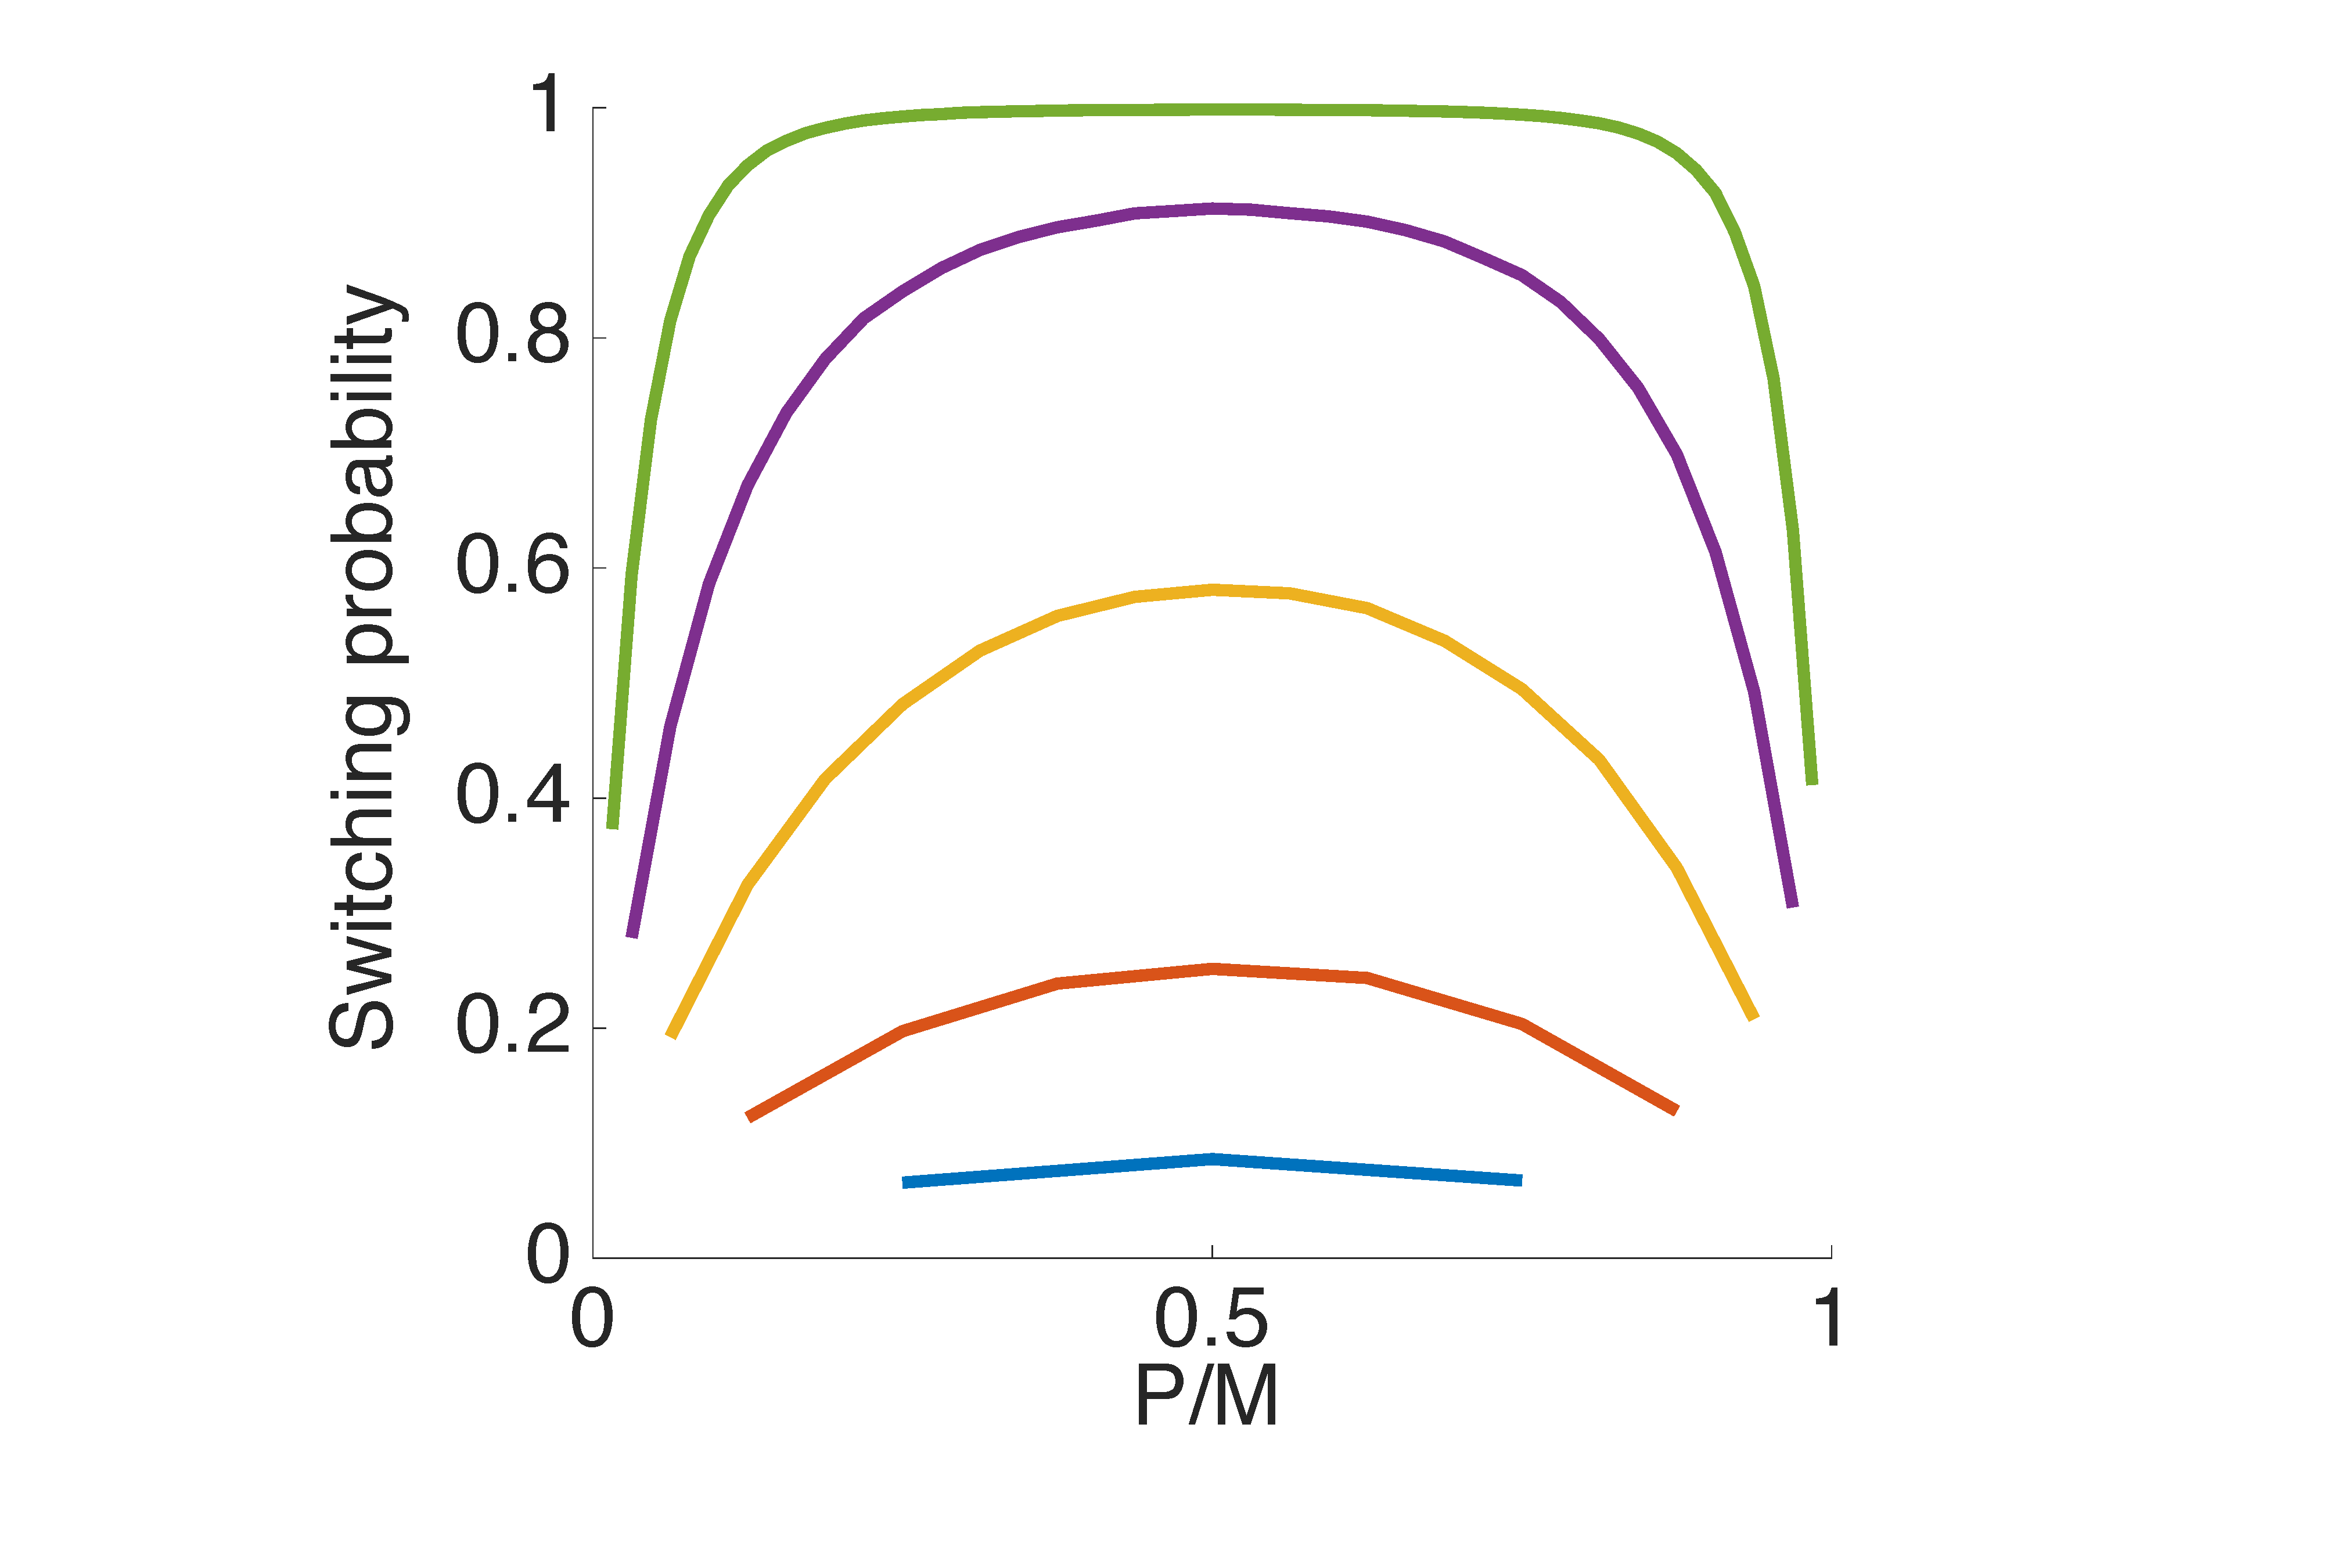
\includegraphics[height=0.75\textwidth]{swtiching_prob_sweep_sigma_3}
		\caption{Limiting log-Normal\label{fig:theSwitchingProb}}
	\end{subfigure}
	~~~~~~~~~~~
	\begin{subfigure}[t]{0.4\textwidth}
		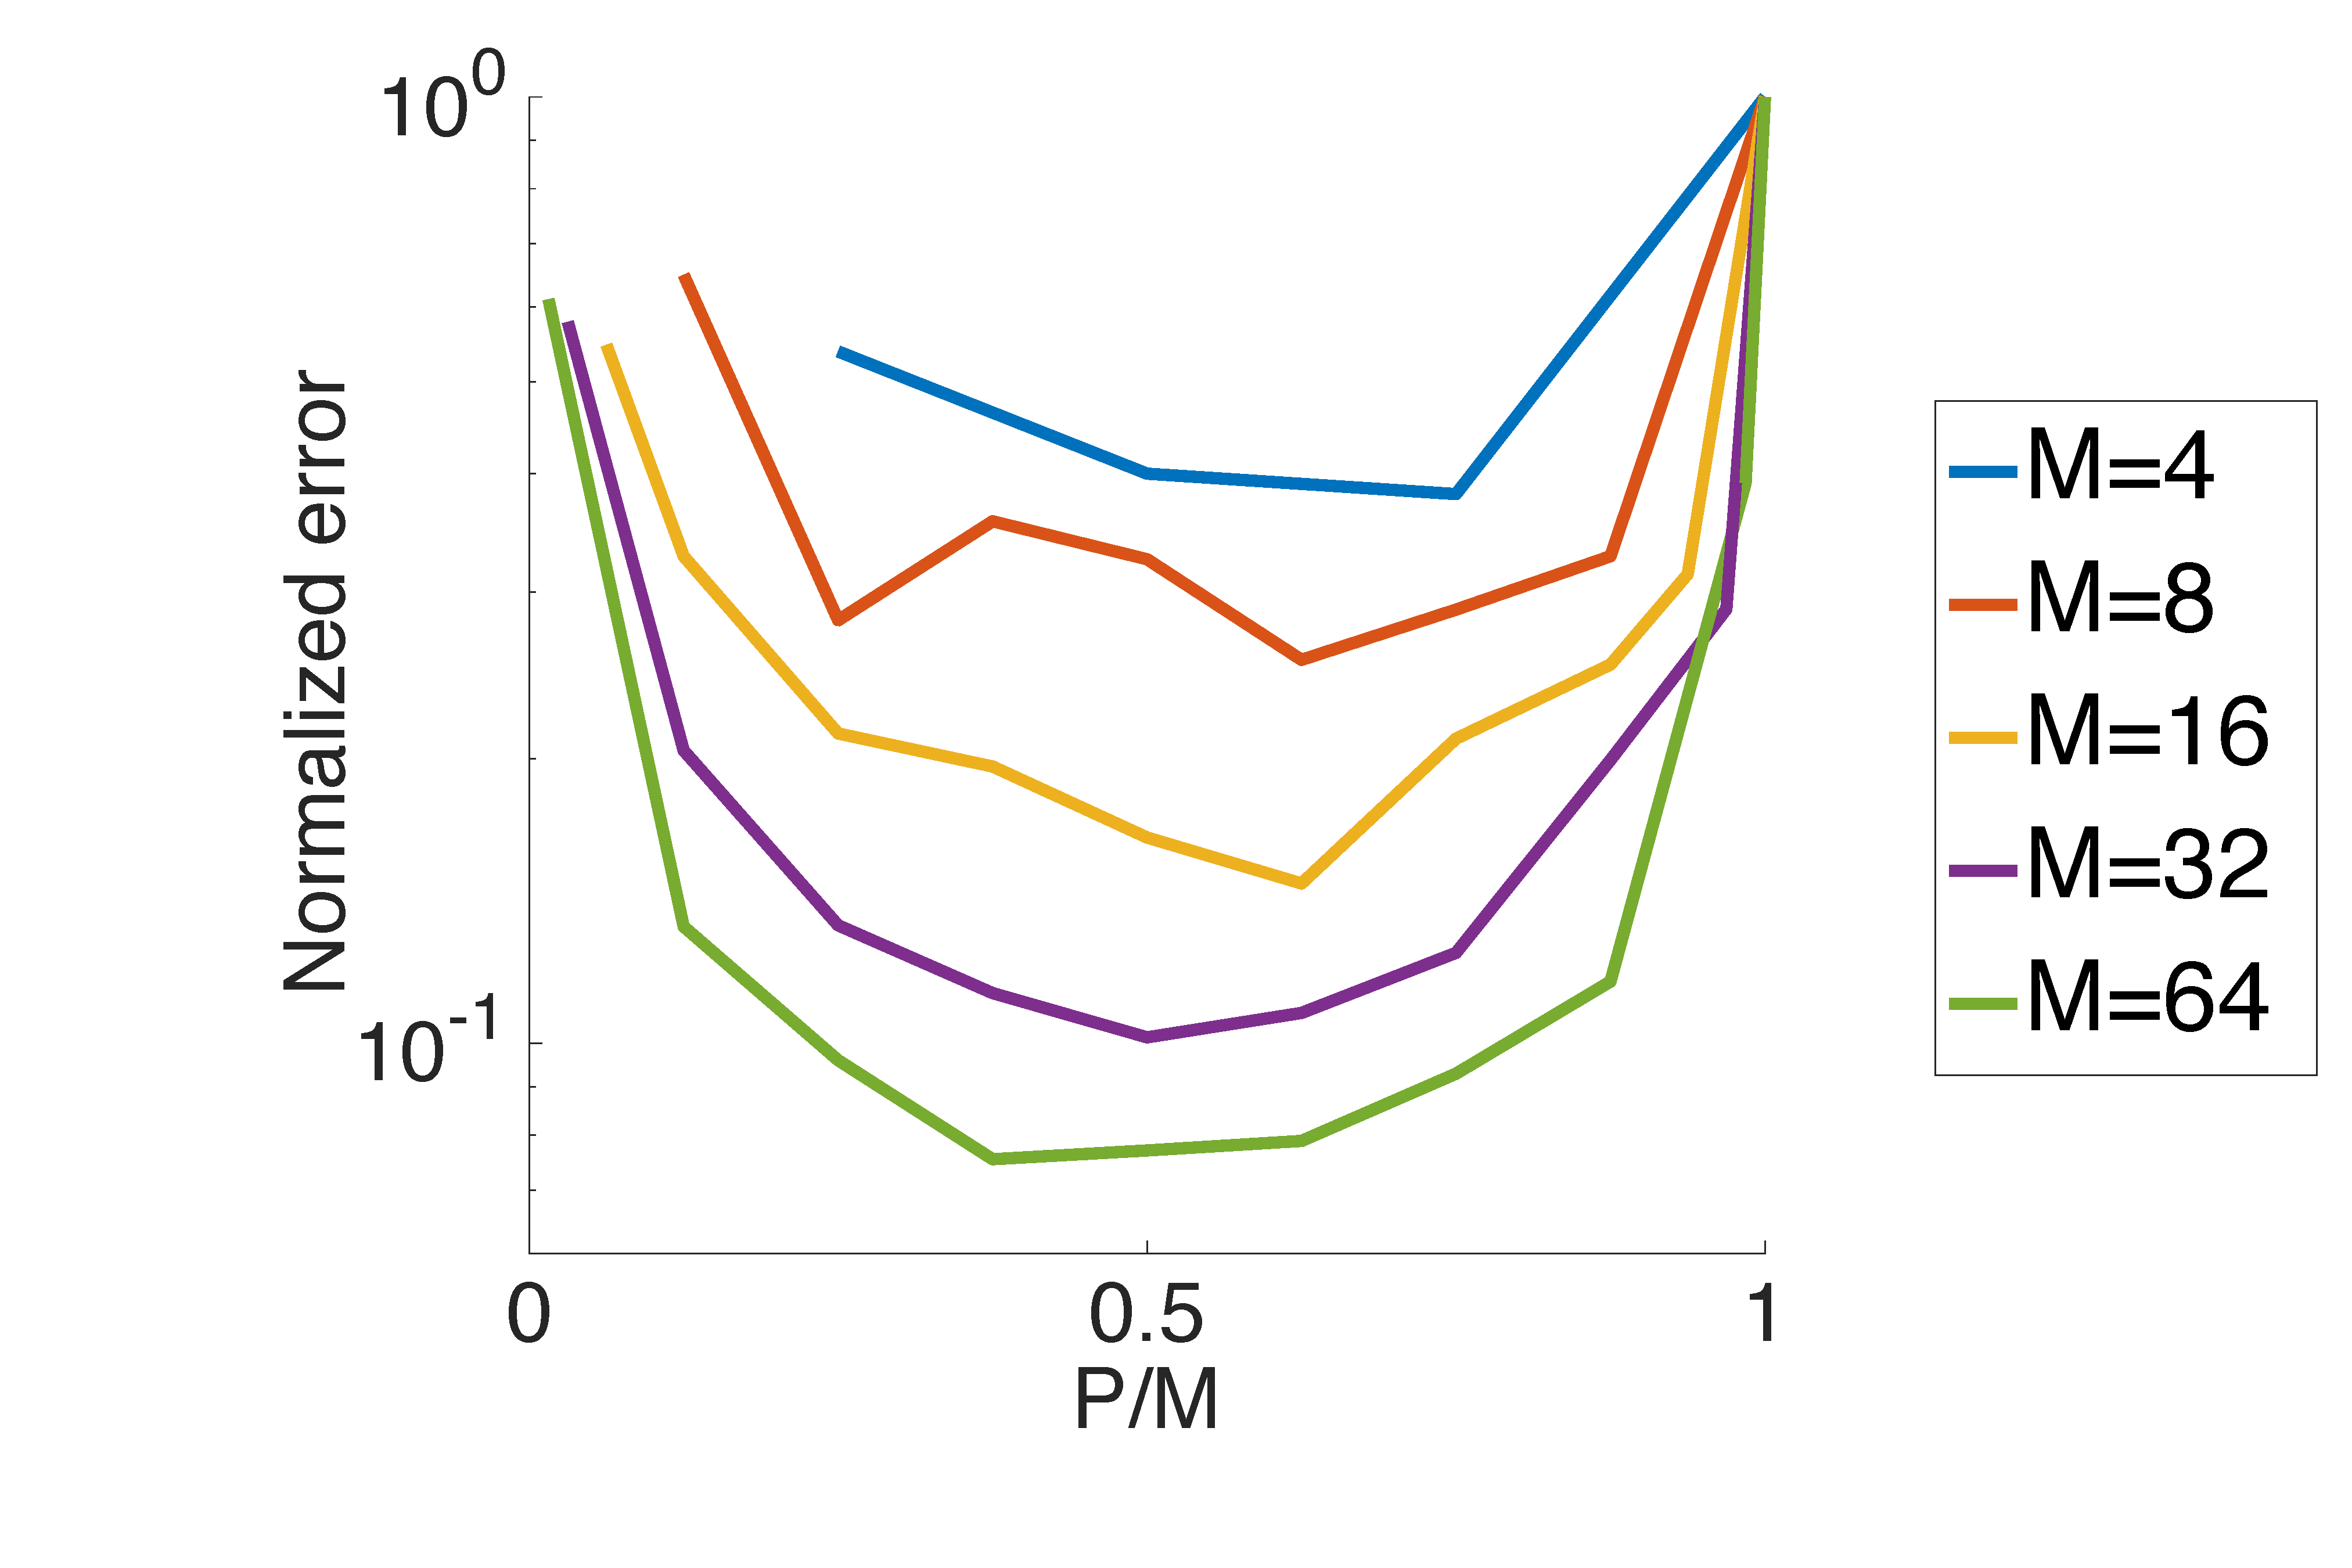
\includegraphics[height=0.75\textwidth]{big_font_p_sweep}
		\caption{Gaussian state space model\label{fig:Psweep}}
	\end{subfigure}
	\caption{a) Estimation of switching probability for different choices of P and M assuming the log-Normal limiting distribution for $\hat{Z}_m$ with $\sigma=3$. b) Median error in mean estimate for different choices of P and M over 10 different synthetic datasets of the linear Gaussian state space model given in~\eqref{eq:LGSS} after 1000 MCMC iterations. Here errors are normalized by the error of a multi-start PG sampler which is a special case of iPMCMC for which $P=M$ (see Section \ref{sec:experiments}).
	}
\end{figure}

%
%\begin{figure}[h]
%
%\end{figure}
%~ %add desired spacing 

In practice we also see that best results are achieved when $P$ makes up roughly half of the nodes, see Figure~\ref{fig:Psweep} for performance on the state space model introduced in~\eqref{eq:LGSS}. Note also that the accuracy seems to be fairly robust with respect to the choice of $P$. % At least for this model, three things are clear from this sweep - firstly the optimal choice for the ratio of P/M is roughly 1/2, secondly that the performance of iPMCMC is relatively robust to changes in P around this optimum and thirdly that as $M$ increases, to relatively more preferable iPMCMC is to the trivial distribution of PG given by $P=M$ (this reason this occurs is discussed in more detail in Section \ref{sec:discussion}). 
%
Based on these results, we set the value of $P=\frac{M}{2}$ for the rest of our experiments.

% !TEX root = ../main.tex

% Numerical experiments section
\section{Experiments}
\label{sec:experiments}

To demonstrate the %validity and
empirical performance of iPMCMC we report experiments on two state space models.  
Although both the models considered are Markovian, we emphasise that iPMCMC goes far beyond this and can be applied to arbitrary graphical models. 
%For exposition we will focus our comparison to the trivial distribution, whereby $M$ independent PMCMC samplers are run in parallel, of PG, particle independent Metropolis-Hastings (PIMH) \cite{andrieuDH2010} and the alternate move PG sampler (APG) \cite{holenstein2009particle}. 
We will focus our comparison on the trivially distributed alternatives, whereby $M$ independent PMCMC samplers are run in parallel--these are PG, particle independent Metropolis-Hastings (PIMH) \cite{andrieuDH2010} and the alternate move PG sampler (APG) \cite{holenstein2009particle}. Comparisons to other alternatives, including independent SMC, serialized implementations of PG and PIMH, and running a mixture of independent PG and PIMH samplers, are provided in Appendix \ref{sec:supp-additionalFigures}.  None outperformed the methods considered here, with the exception of running a serialized PG implementation with an increased number of particles, requiring significant additional memory ($O(MN)$ as opposed to $O(M+N)$).

In PIMH a new particle set is proposed at each \mcmc step using an independent \smc sweep, which is then either accepted or rejected using the standard Metropolis-Hastings acceptance ratio. % \cite{andrieuDH2010}. %\cite{hastings1970monte}. 
APG interleaves PG steps with PIMH steps
%, alternating between \csmc updates and a Metropolis-Hastings step with an independent \smc proposal,
in an attempt to overcome the issues caused by path degeneracy in PG.  We refer to the trivially distributed versions of these algorithms as multi-start PG, PIMH and APG respectively (mPG, mPIMH and mAPG). 
We use Rao-Blackwellization, as described in \ref{sec:allparticles}, to average over all the generated particles for all methods, weighting the independent Markov chains equally for mPG, mPIMH and mAPG. We note that mPG is a special case of iPMCMC for which $P=M$.  For simplicity, multinomial resampling was used in the experiments, with the prior transition distribution of the latent variables taken for the proposal.  $M=32$ nodes and $N=100$ particles were used unless otherwise stated.  Initialization of the retained particles for iPMCMC and mPG was done by using standard SMC sweeps.

\subsection{Linear Gaussian State Space Model}
\label{sec:LGSS}
We first consider a linear Gaussian state space model (LGSSM) with 3 dimensional latent states $x_{1:T}$, 20 dimensional observations $y_{1:T}$ and dynamics given by %\cn{It seems you use deterministic initial conditions for $x_0$, reformulate the model so you have a prior $\mu(x_1)$ instead? (also follows notation above)}
\begin{subequations}
	\label{eq:LGSS}
	\begin{align}
	x_1 & \sim \mathcal{N} \left(\mu, V\right) \label{eq:LGSSa}\\
	x_t & = \alpha x_{t-1} + \delta_{t-1} \quad & \delta_{t-1} \sim \mathcal{N} \left(0, \Omega\right) \label{eq:LGSSb}\\
	y_t & = \beta x_{t} + \varepsilon_{t} \quad & \varepsilon_{t} \sim \mathcal{N} \left(0, \Sigma\right).
	\label{eq:LGSSc}
	\end{align}
\end{subequations}
We set $\mu = [0, 1, 1]^T$, $V = 0.1 \; \mathbf{I}$, $\Omega = \mathbf{I}$ and $\Sigma = 0.1 \; \mathbf{I}$ where $\mathbf{I}$ represents the identity matrix.  The constant transition matrix, $\alpha$, corresponds to successively applying rotations of $\frac{7\pi}{10}$, $\frac{3\pi}{10}$ and $\frac{\pi}{20}$ about the first, second and third dimensions of $x_{t-1}$ respectively followed by a scaling of $0.99$ to ensure that the dynamics remain stable.  A total of 10 different synthetic datasets of length $T=50$ were generated by simulating from~\eqref{eq:LGSSa}--\eqref{eq:LGSSc}, each with a different emission matrix $\beta$ generated by sampling each column independently from a symmetric Dirichlet distribution with concentration parameter 0.2.

Figure \ref{fig:meanConv} shows convergence in the estimate of the latent variable means to the ground-truth solution for iPMCMC and the benchmark algorithms as a function of MCMC iterations.  It shows that iPMCMC comfortably outperforms the alternatives from around 200 iterations onwards, with only iPMCMC and mAPG demonstrating behaviour consistent with the Monte Carlo convergence rate, suggesting that mPG and mPIMH are still far from the ergodic regime.  Figure \ref{fig:meanPos} shows the same errors after $10^4$ MCMC iterations as a function of position in state sequence.  This demonstrates that iPMCMC outperformed all the other algorithms for the early stages of the state sequence, for which mPG performed particularly poorly. Toward the end of state sequence, iPMCMC, mPG and mAPG all gave similar performance, whilst that of mPIMH was significantly worse.


\begin{figure*}[t]
	\centering
	\begin{subfigure}[t]{0.49\textwidth}
		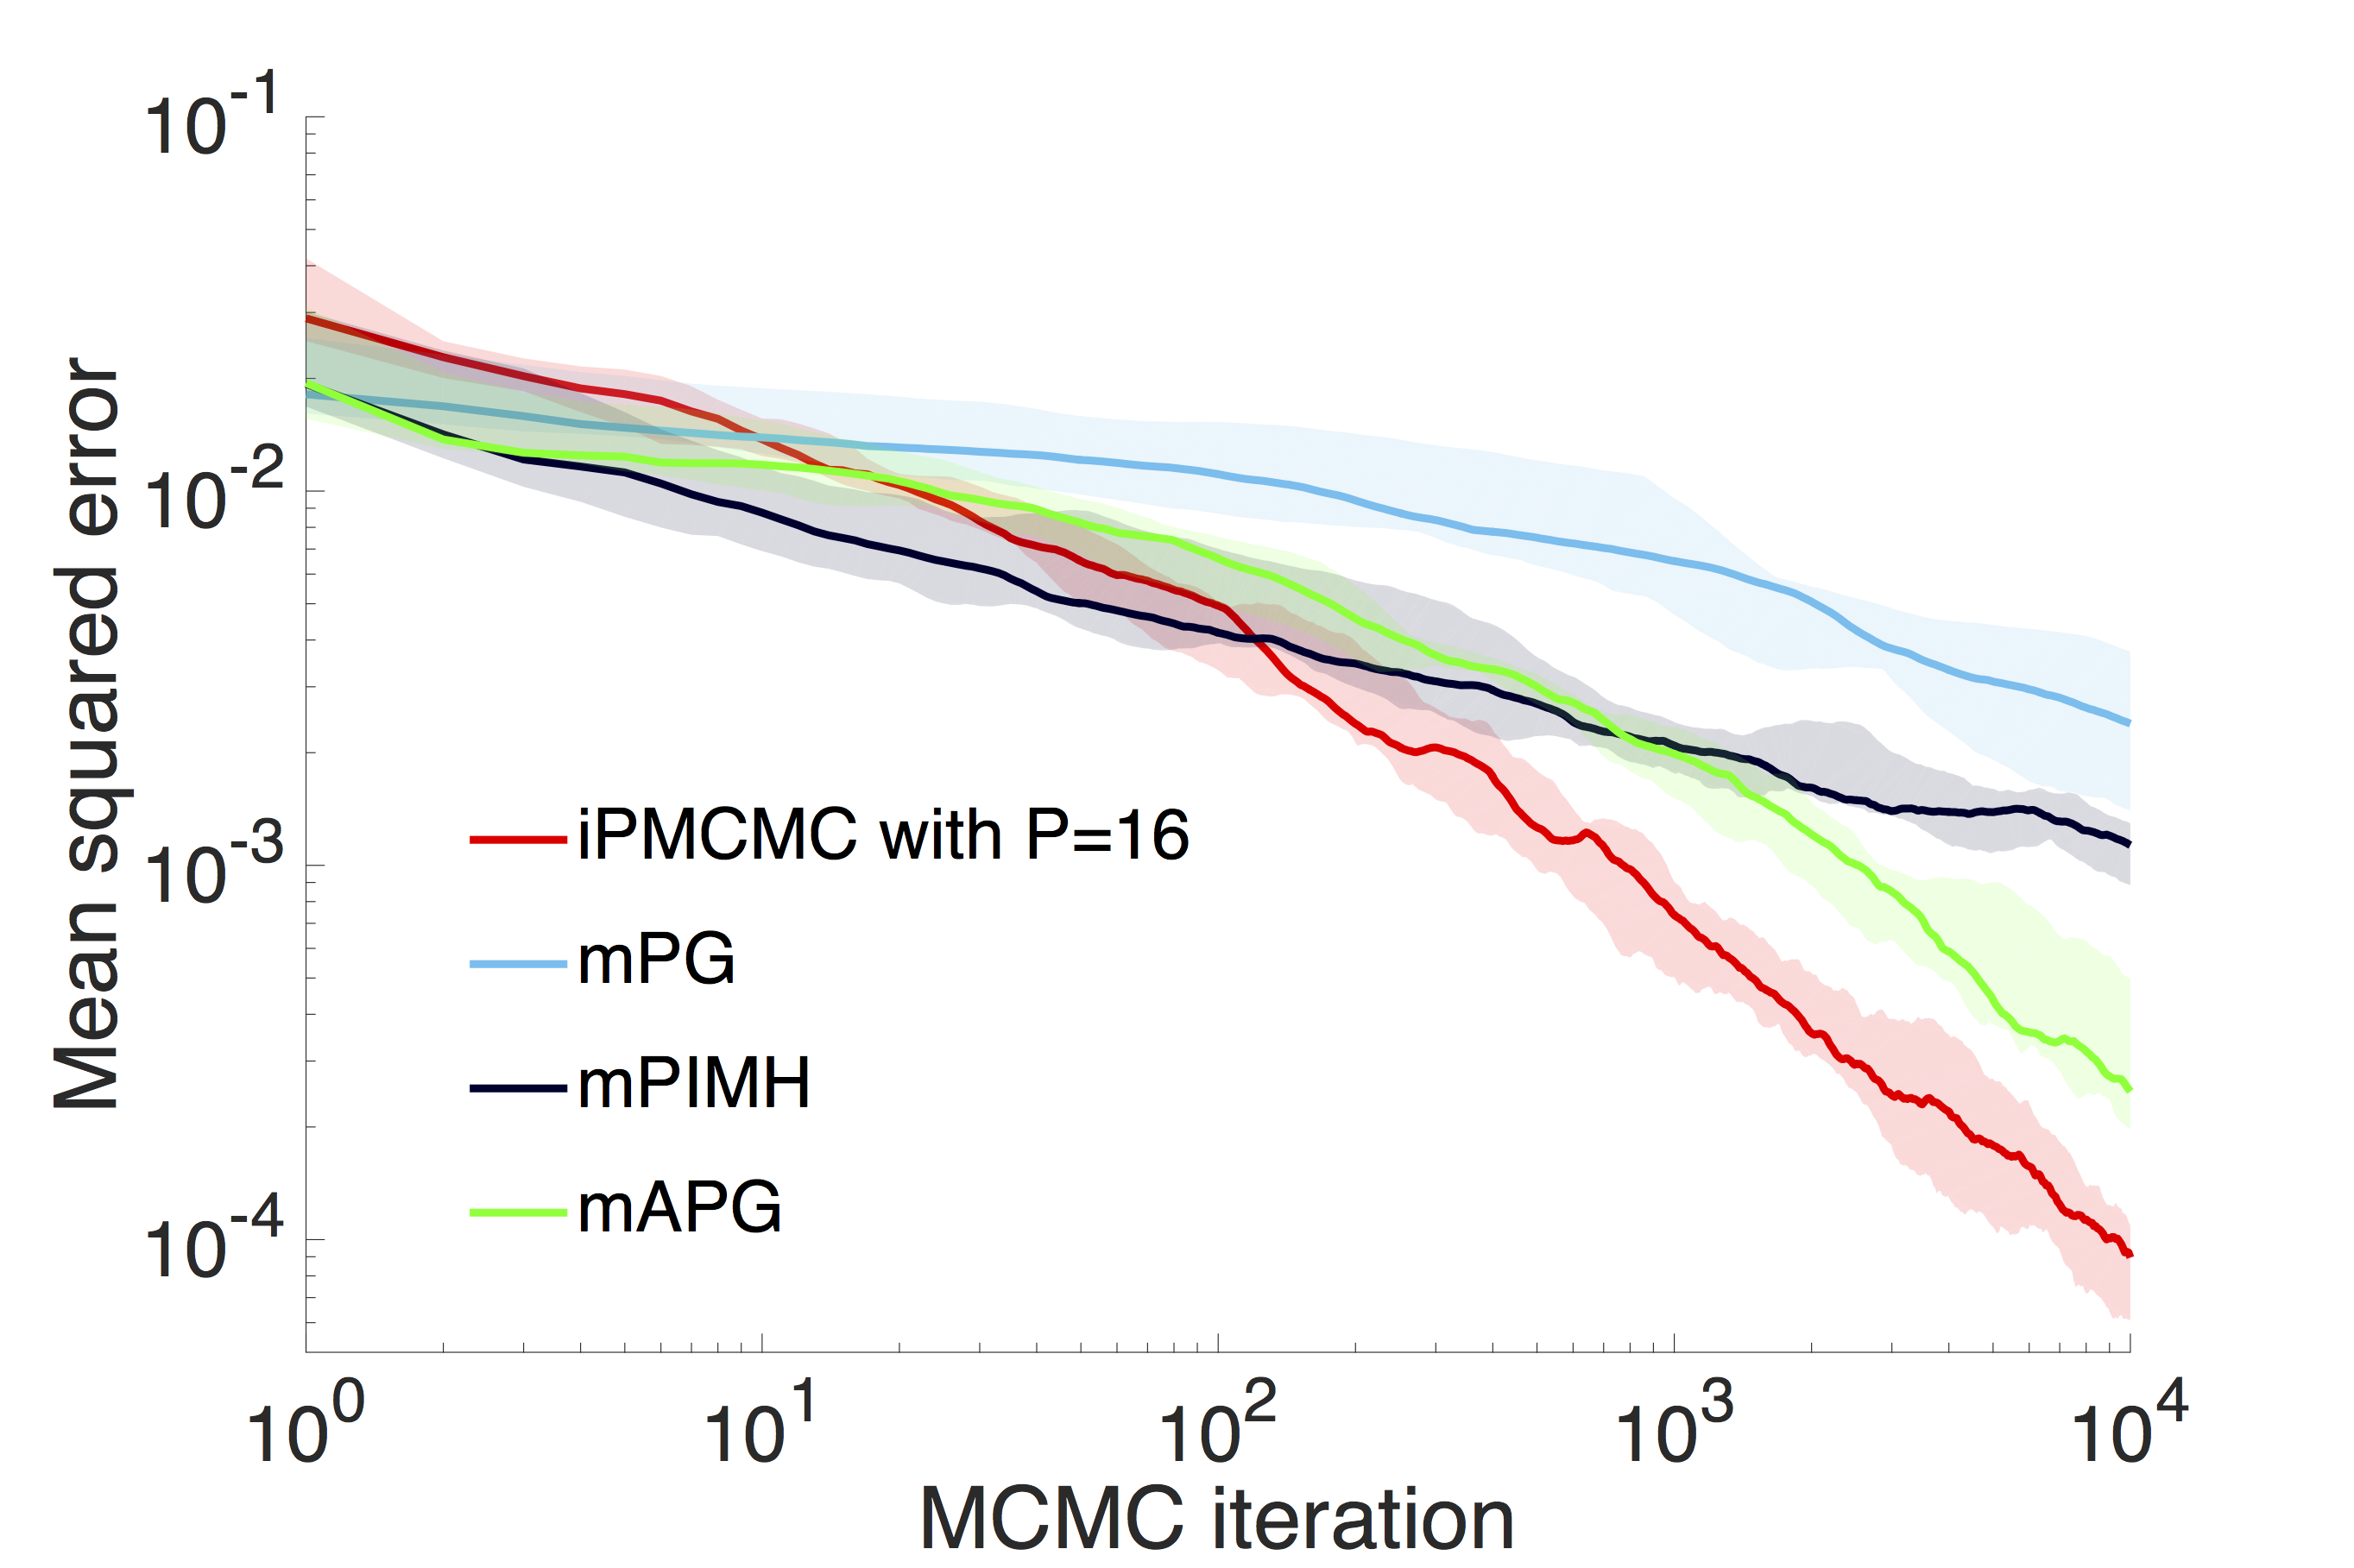
\includegraphics[width=\textwidth]{mean_conv_lss}
		\caption{Convergence in mean for full sequence}
		\label{fig:meanConv}
	\end{subfigure}
	~  %add desired spacing between images, e. g. ~, \quad, \qquad, \hfill etc. 
	%(or a blank line to force the subfigure onto a new line)
	\begin{subfigure}[t]{0.49\textwidth}
		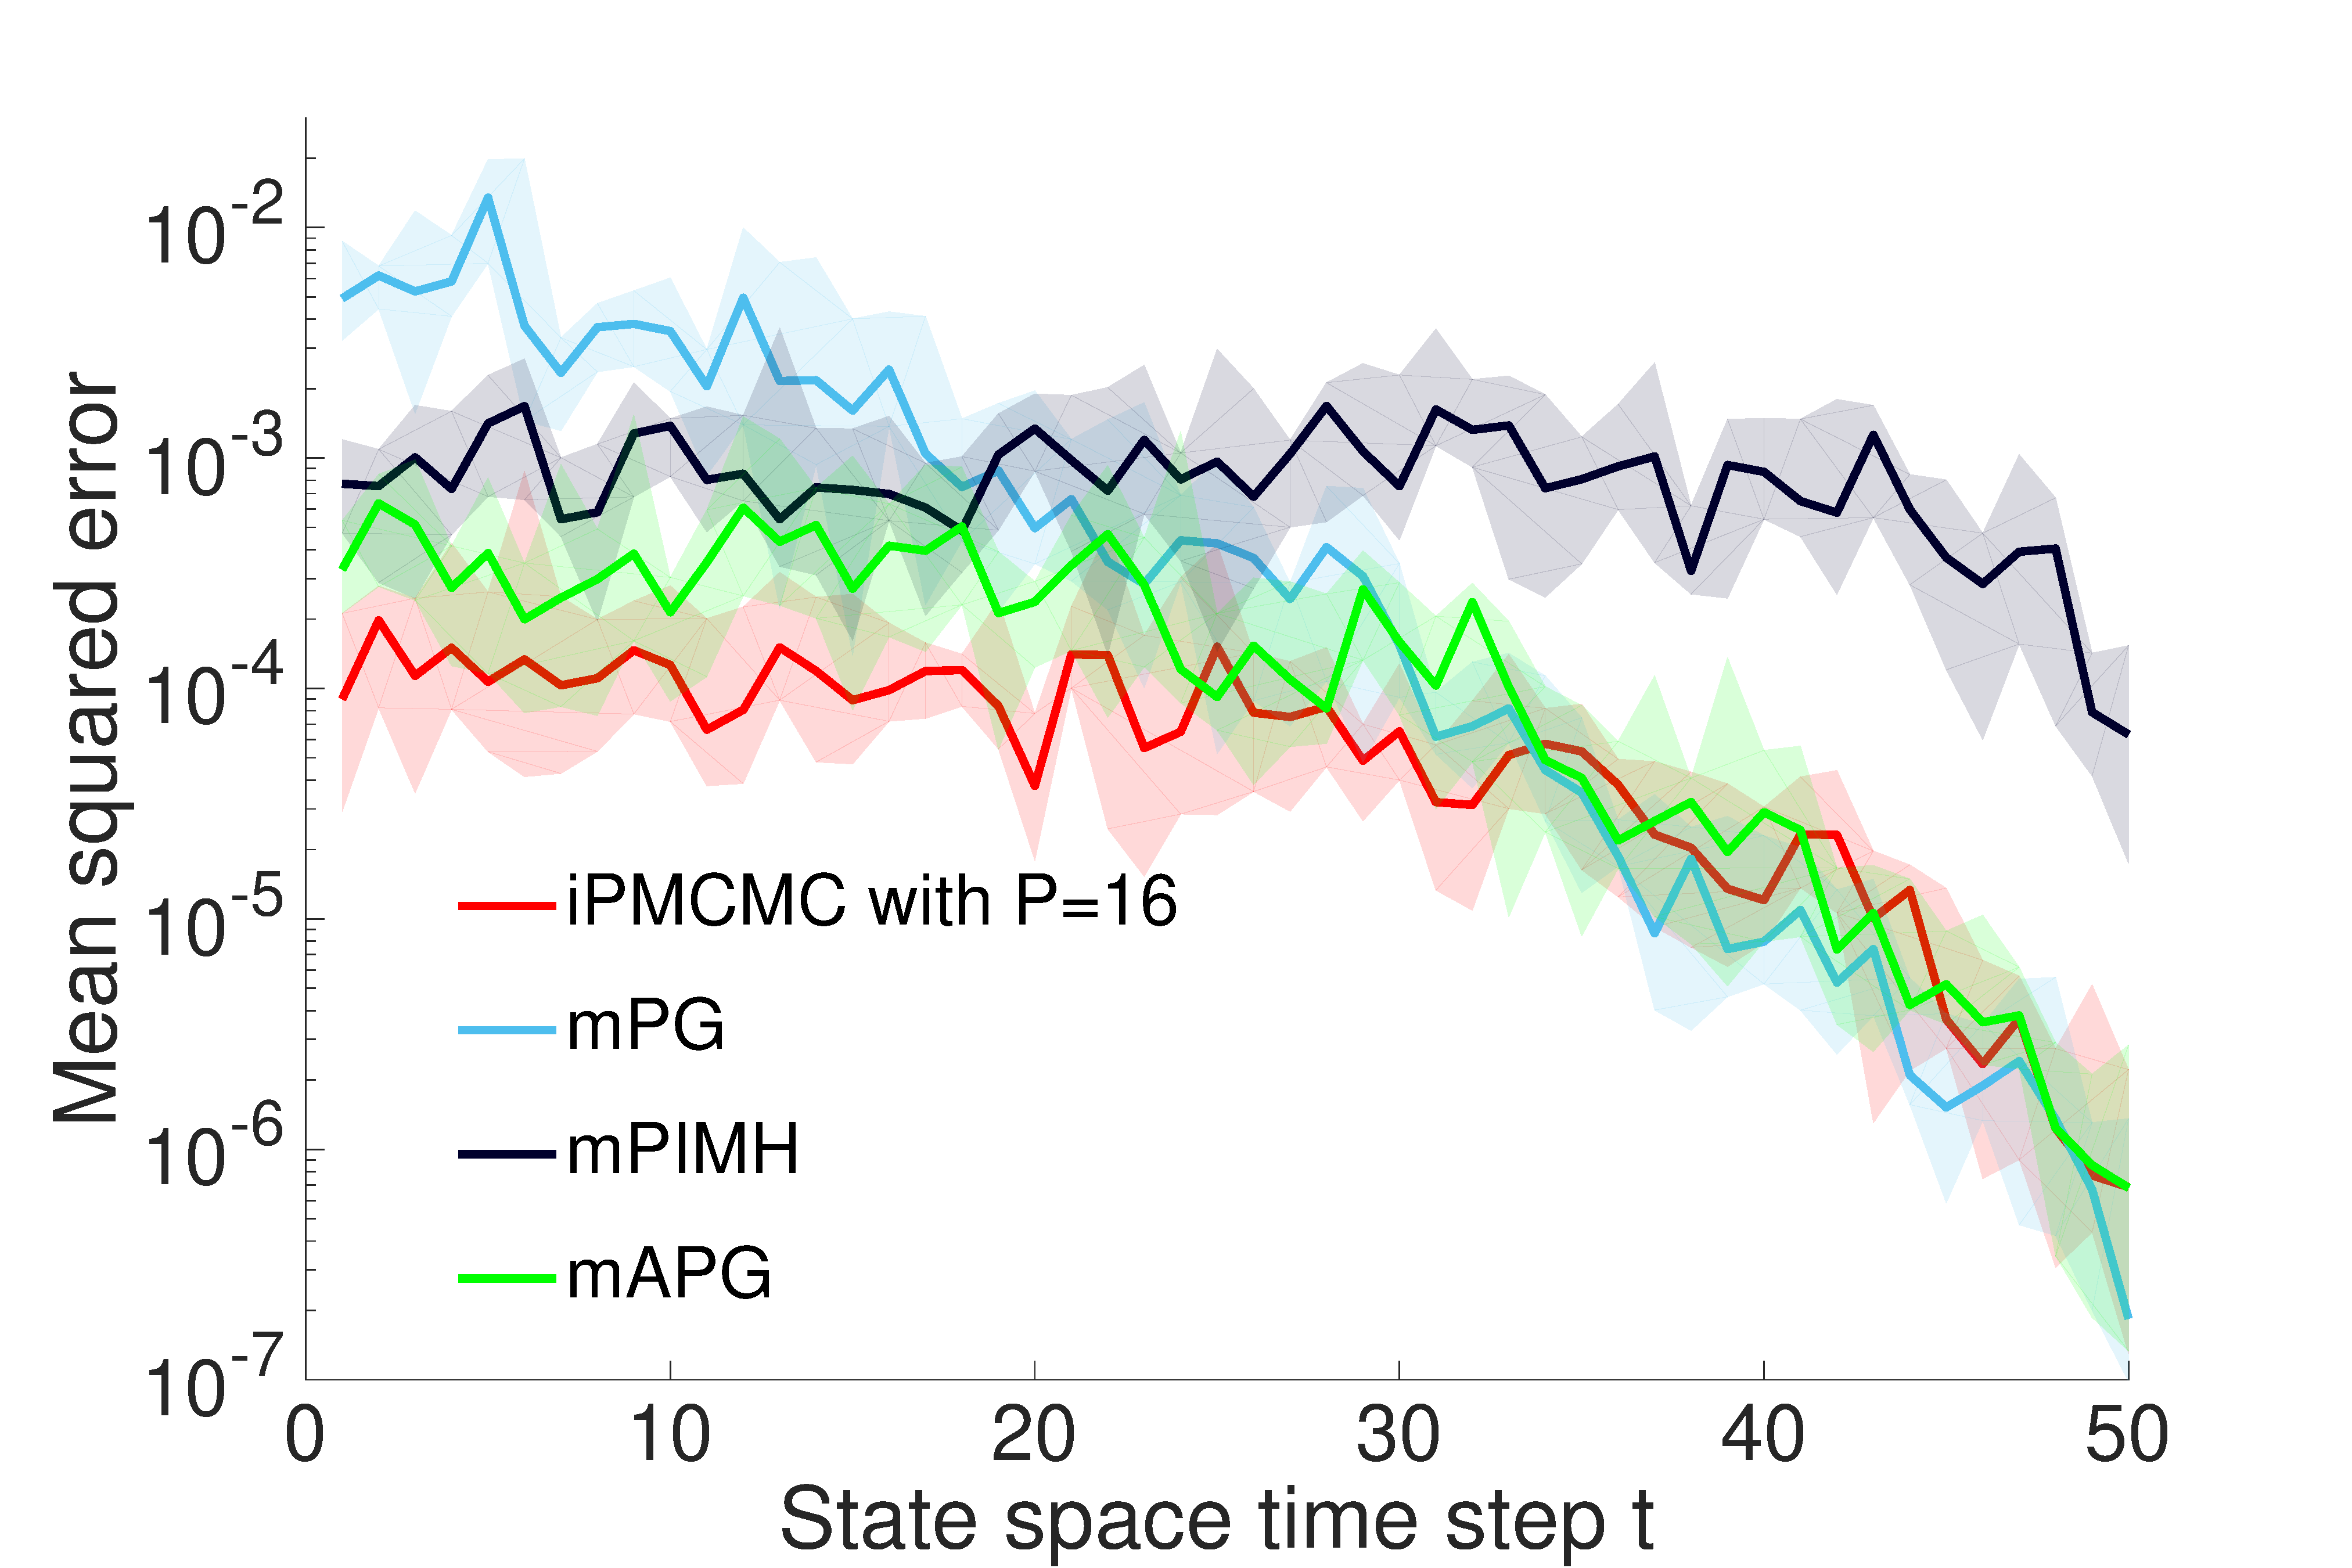
\includegraphics[width=\textwidth]{mean_pos_lss}
		\caption{Final error in mean for latent marginals}
		\label{fig:meanPos}
	\end{subfigure}
	
	%	\begin{subfigure}[t]{0.49\textwidth}
	%		\includegraphics[width=\textwidth]{std_conv_lss}
	%		\caption{Convergence in standard deviation for full sequence}
	%		\label{fig:stdConv}
	%	\end{subfigure}
	%	~ %add desired spacing between images, e. g. ~, \quad, \qquad, \hfill etc. 
	%	%(or a blank line to force the subfigure onto a new line)
	%	\begin{subfigure}[t]{0.49\textwidth}
	%		\includegraphics[width=\textwidth]{std_pos_lss}
	%		\caption{Final error in standard deviation for latent marginals}
	%		\label{fig:stdPos}
	%	\end{subfigure}	
	\caption{Mean squared error averaged over all dimensions and steps in the state sequence as a function of MCMC iterations (left) and mean squared error after $10^4$ iterations averaged over dimensions as function of position in the state sequence (right) for \eqref{eq:LGSS} with 50 time sequences.  The solid line shows the median error across the 10 tested synthetic datasets, while the shading shows the upper and lower quartiles.  Ground truth was calculated using the Rauch--Tung--Striebel smoother algorithm \cite{rauch1965maximum}. 
		\label{fig:groundTruth}}
\end{figure*}

\begin{figure*}[t]
	\centering
	\begin{subfigure}[t]{0.49\textwidth}
		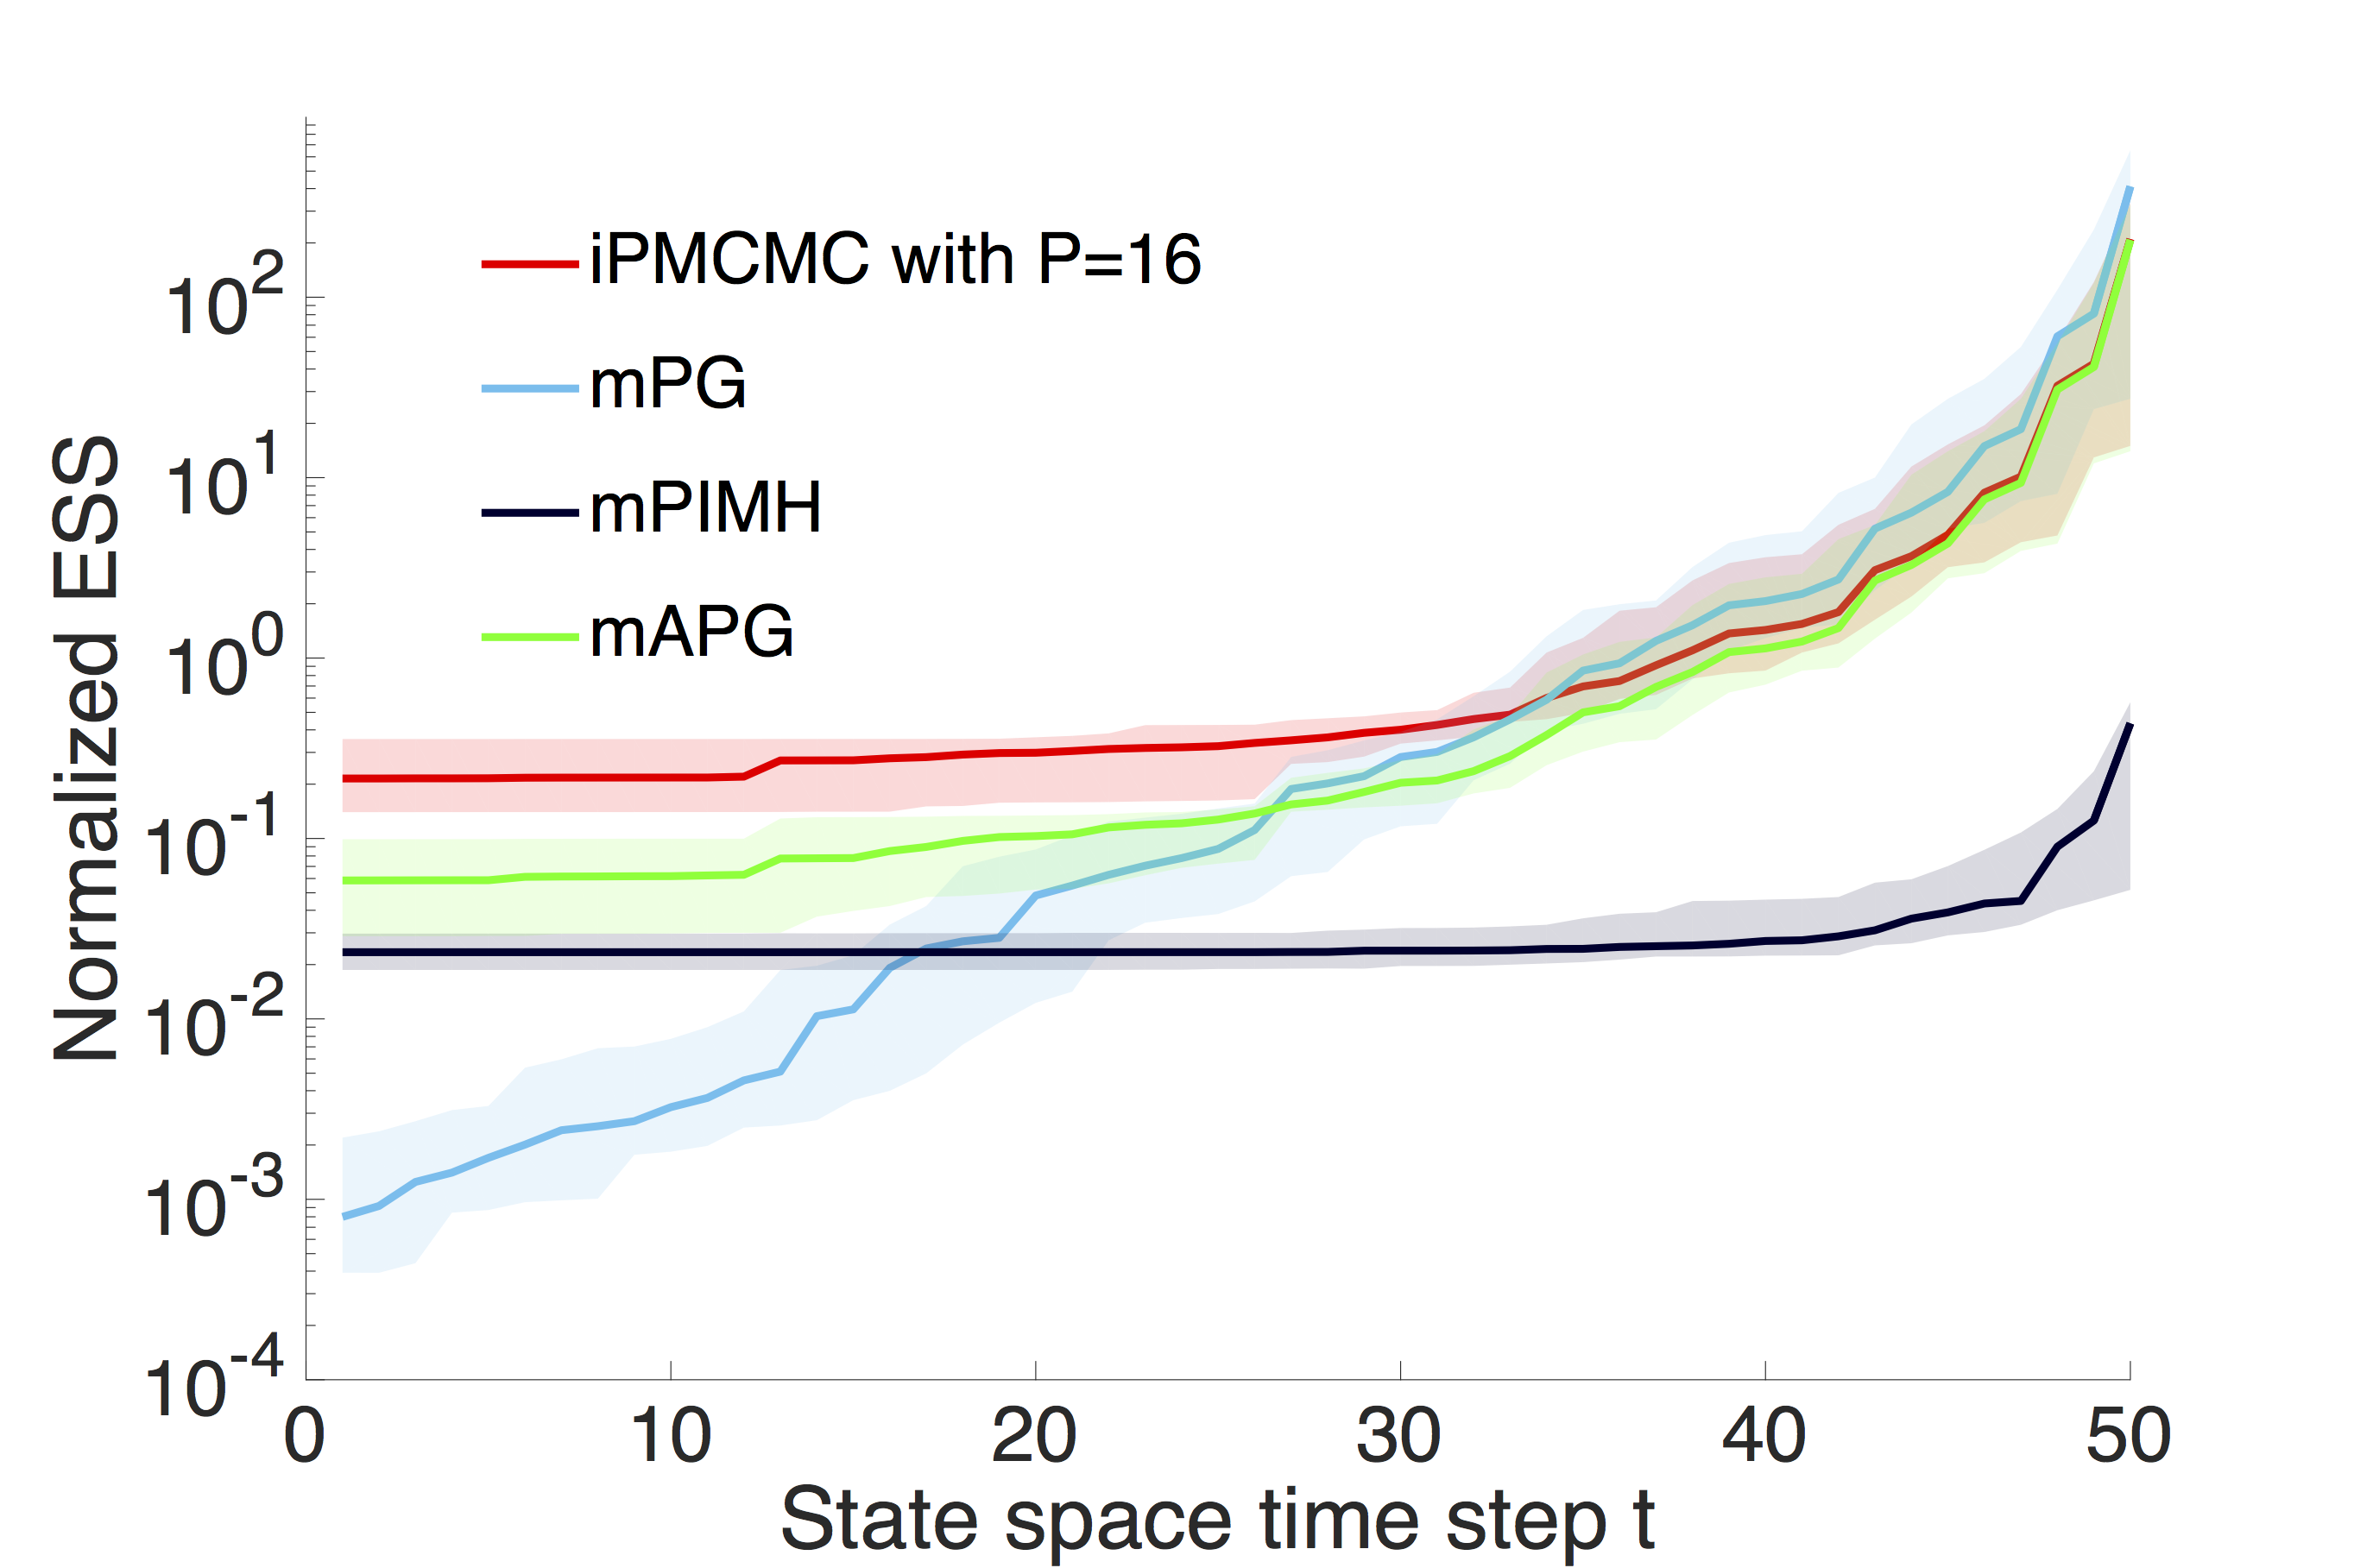
\includegraphics[width=\textwidth]{ess_lss}
		\caption{LGSSM}
	\end{subfigure}
	~ %add desired spacing between images, e. g. ~, \quad, \qquad, \hfill etc. 
	%(or a blank line to force the subfigure onto a new line)
	\begin{subfigure}[t]{0.49\textwidth}
		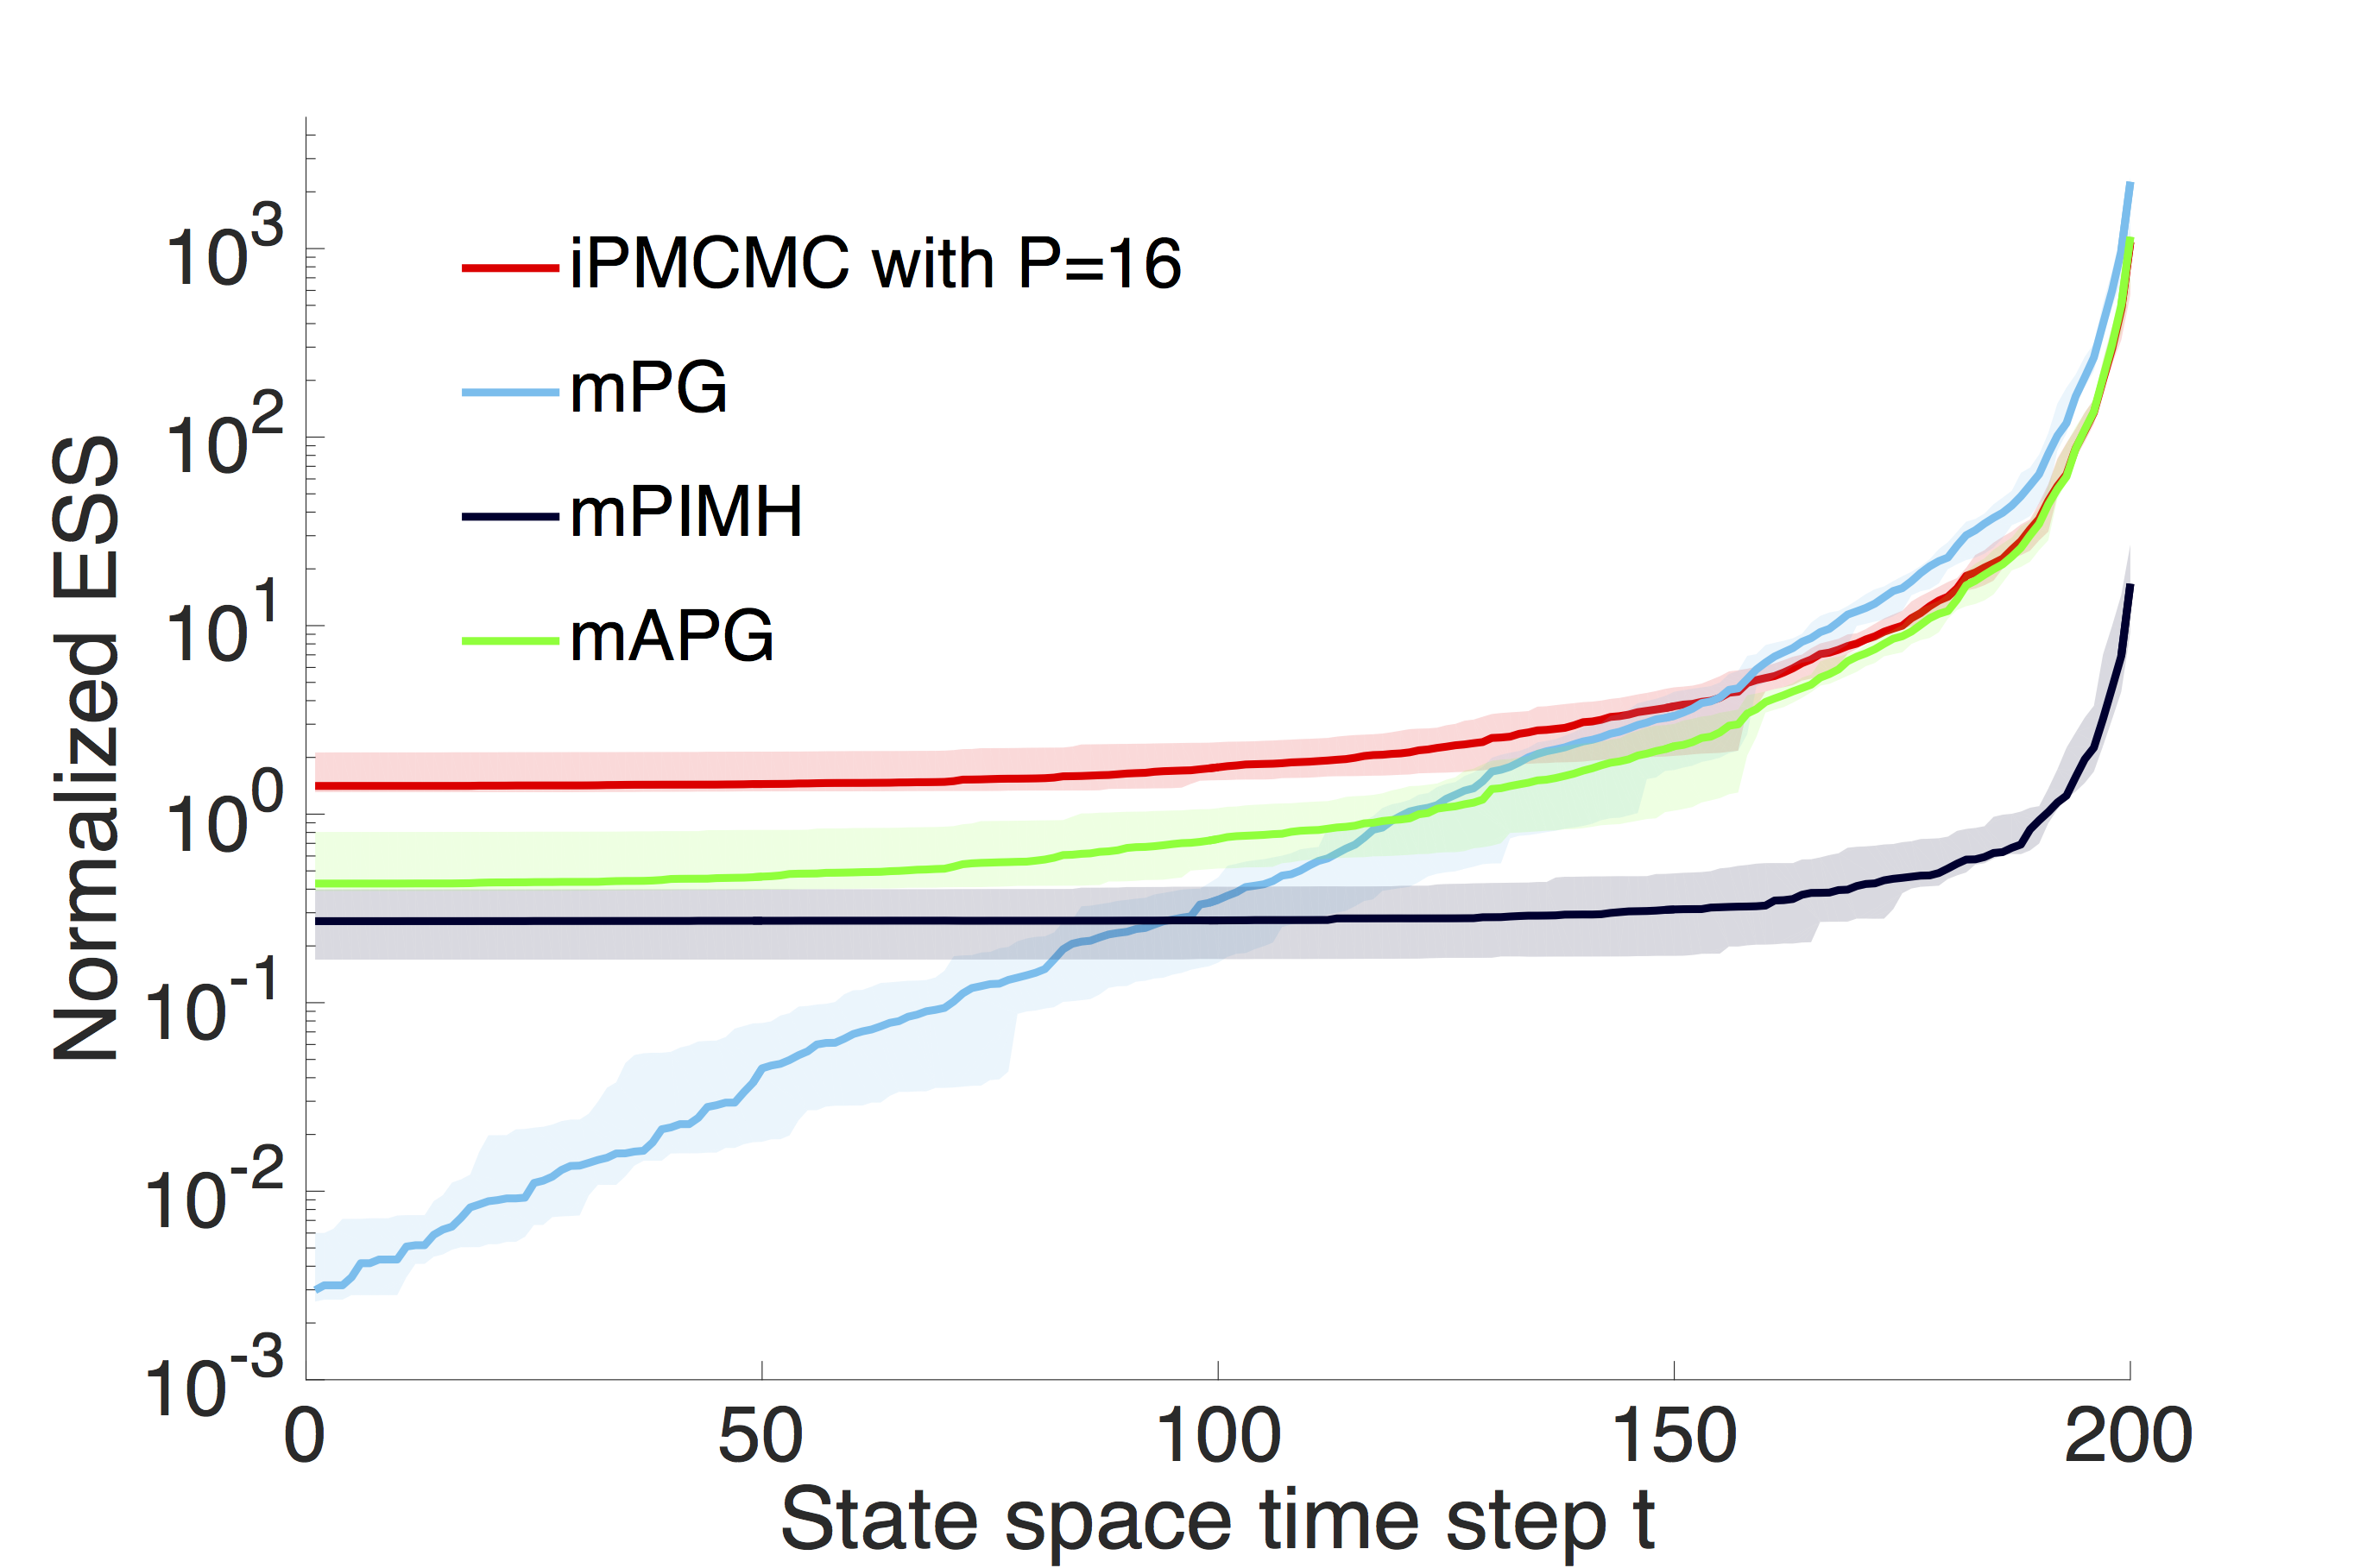
\includegraphics[width=\textwidth]{ess_nlss}
		\caption{NLSSM}
	\end{subfigure}
	
	\caption{Normalized effective sample size  (NESS) for LGSSM (left) and NLSSM (right).
		\label{fig:ESS}}
\end{figure*}

\subsection{Nonlinear State Space Model}
\label{sec:nlss}

We next consider the one dimensional nonlinear state space model (NLSSM) considered by, among others, \citet{gordon1993novel,andrieuDH2010}
\begin{subequations}
	\label{eq:NLSS}
	\begin{align}
	x_1 & \sim \mathcal{N} \left(\mu, v^2\right) \label{eq:NLSSa}\\
	x_t & = \frac{x_{t-1}}{2} + 25 \frac{x_{t-1}}{1+x_{t-1}^2} + 8 \cos \left(1.2t\right) + \delta_{t-1} \label{eq:NLSSb} \\
	y_t & = \frac{{x_{t}}^2}{20} + \varepsilon_{t} \label{eq:NLSSc}
	\end{align}
\end{subequations}
where $\delta_{t-1} \sim \mathcal{N} \left(0, \omega^2\right)$ and $\varepsilon_{t} \sim \mathcal{N} \left(0, \sigma^2\right)$.  We set the parameters as $\mu = 0$, $v=\sqrt{5}$, $\omega = \sqrt{10}$ and $\sigma = \sqrt{10}$.  Unlike the LGSSM, this model does not have an analytic solution and therefore one must resort to approximate inference methods. 
% such as sampling.
Further, the multi-modal nature of the latent space makes full posterior inference over $x_{1:T}$ challenging for long state sequences. 

\begin{figure*}[t]
	\centering
	%\begin{subfigure}[t]{0.99\textwidth}
	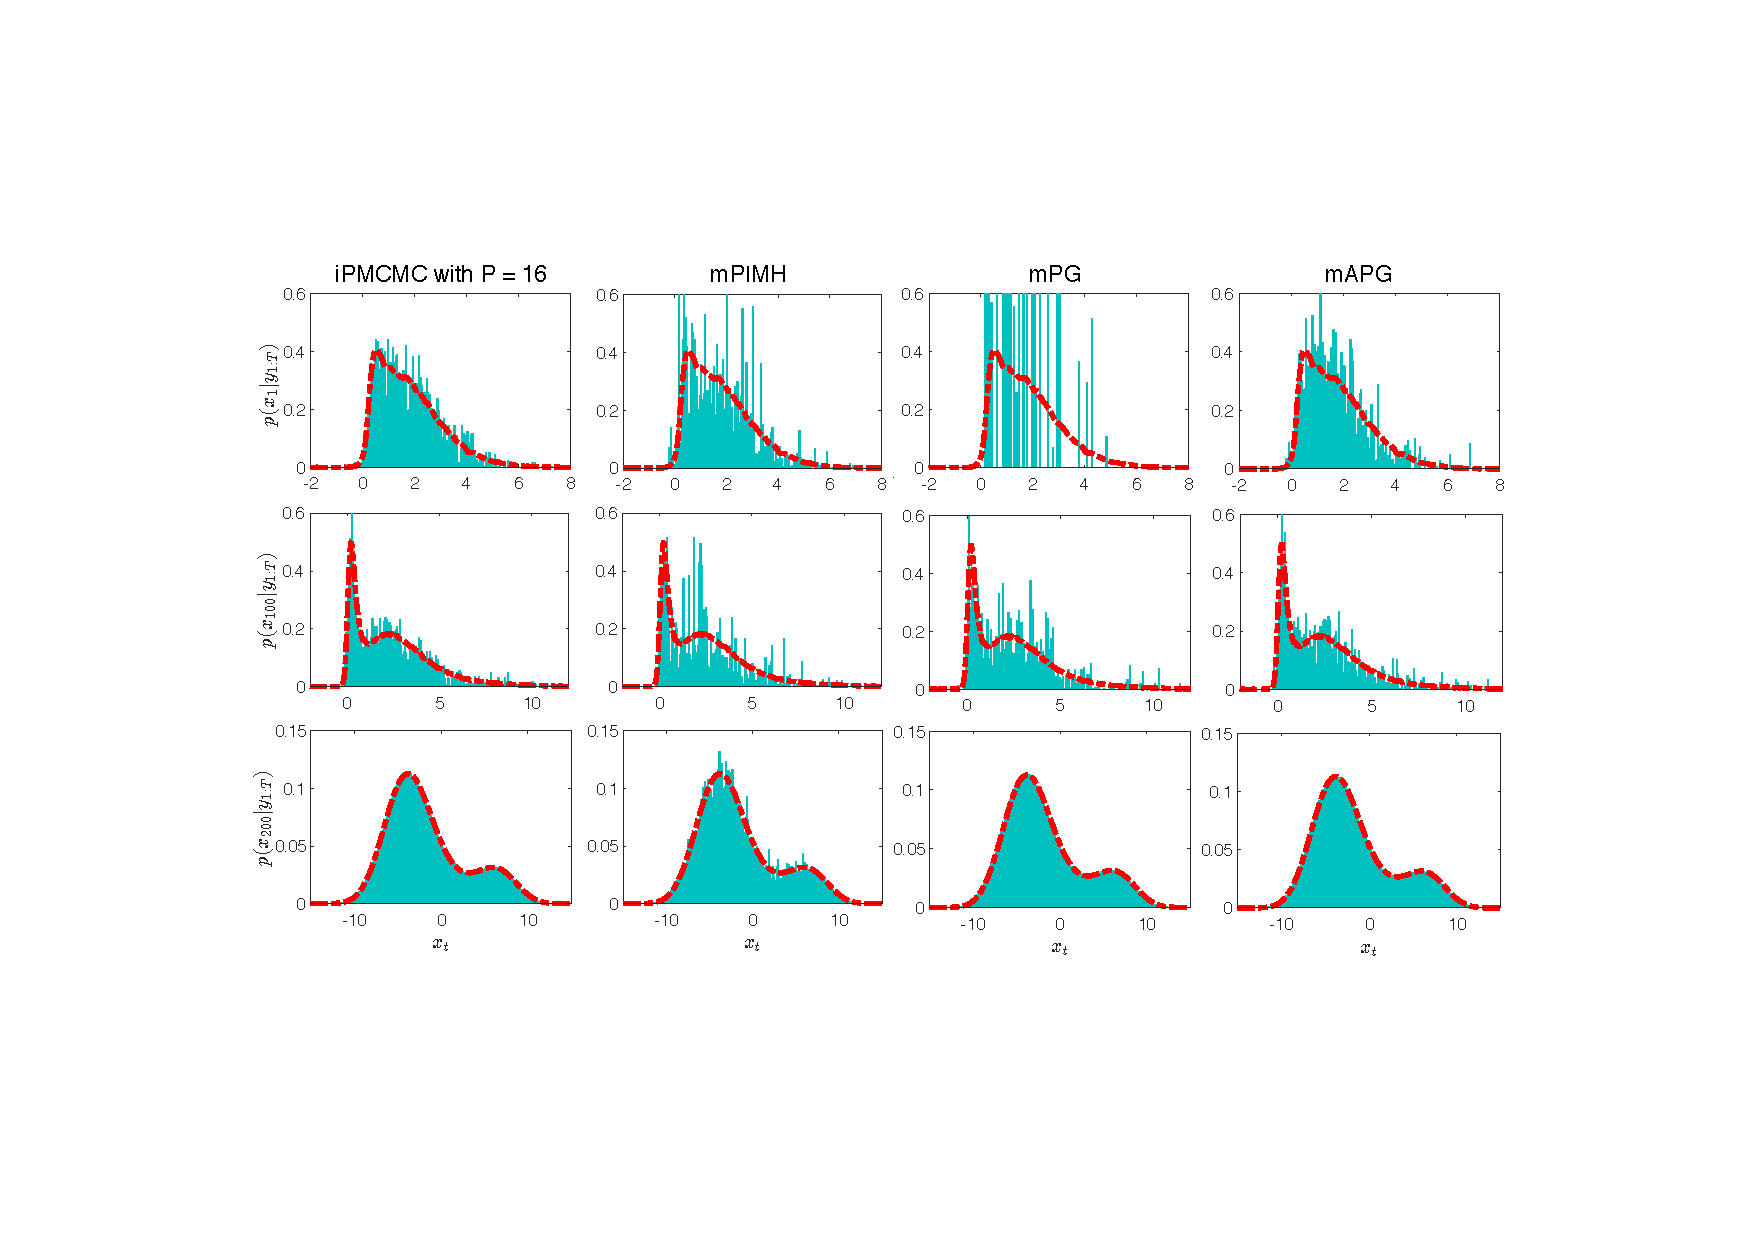
\includegraphics[width=1\textwidth]{nlss_histograms_minus_190.pdf}
	%\end{subfigure}
	\caption{Histograms of generated samples at $t=1, 100, \text{ and } 200$ for a single dataset generated from \eqref{eq:NLSS} with $T=200$.  Dashed red line shows an approximate estimate of the ground truth, found by running a kernel density estimator on the combined samples from a small number of independent SMC sweeps, each with $10^7$ particles. \label{fig:nlssHists}}
\end{figure*}

To examine the relative mixing of iPMCMC we calculate an effective sample size (ESS) for different steps in the state sequence.  In order to calculate the ESS, we condensed identical samples as done in for example \cite{vandemeent_aistats_2015}.  Let 
\begin{align*}
u_{t}^k \in \{x_{t,m}^{i}[r]\}^{i=1:N,r=1:R}_{m=1:M}, \quad \forall k \in 1 \dots K, \; t \in 1 \dots T
\end{align*} 
denote the unique samples of $x_t$ generated by all the nodes and sweeps of particular algorithm after $R$ iterations, where $K$ is the total number of unique samples generated.  The weight assigned to these unique samples, $v_t^{k}$, is given by the combined weights of all particles for which $x_t$ takes the value $u_{t}^k$:
\begin{align}
v_t^{k} = \sum_{r=1}^{R} \sum_{m=1}^{M} \sum_{i=1}^{N} \bar{w}_{t,m}^{i,r} \eta_{m}^{r} \delta_{x_{t,m}^{i}[r]}(u_{t}^{k})
\end{align}
where $\delta_{x_{t,m}^{i}[r]}(u_{t}^{k})$ is the Kronecker delta function and $\eta_{m}^{r}$ is a node weight.  For iPMCMC the node weight is given by as per the Rao-Blackwellized estimator described in Section~\ref{sec:allparticles}. For mPG and mPIMH, $\eta_{m}^{r}$ is simply $\frac{1}{RM}$,
as samples from the different nodes are weighted equally in the absence of interaction. 
Finally we define the effective sample size as $\text{ESS}_t = \left(\textstyle\sum_{k=1}^K \left(v_t^{k}\right)^2\right)^{-1}$.
%\begin{align}
%\label{eq:ESS}
%\text{ESS}_t = \left(\textstyle\sum_{k=1}^K \left(v_t^{k}\right)^2\right)^{-1}.
%\end{align}

Figure \ref{fig:ESS} shows the ESS for the LGSSM and NLSSM as a function of position in the state sequence.  For this, we omit the samples generated by the initialization step as this SMC sweep is common to all the tested algorithms.  We further normalize by the number of MCMC iterations so as to give an idea of the rate at which unique samples are generated.  These show that for both models the ESS of iPMCMC, mPG and mAPG is similar towards the end of the space sequence, but that iPMCMC outperforms all the other methods at the early stages. The ESS of mPG was particularly poor at early iterations.  PIMH performed poorly throughout, reflecting the very low observed acceptance ratio of around $7.3\%$ on average. 
%The lack of Monte Carlo convergence rate appearing in Figure \ref{fig:meanConv} also suggests this acceptance ratio is yet to converge, with the value in the ergodic regime likely to be even lower.   

It should be noted that the ESS is not a direct measure of performance for these models.  For example, the equal weighting of nodes is likely to make the ESS artificially high for mPG, mPIMH and mAPG, when compared with methods such as iPMCMC that assign a weighting to the nodes at each iteration.  To acknowledge this, we also plot histograms for the marginal distributions of a number of different position in the state sequence as shown in Figure \ref{fig:nlssHists}.  These confirm that iPMCMC and mPG have similar performance at the latter state sequence steps, whilst iPMCMC is superior at the earlier stages, with mPG producing almost no more new samples than those from the initialization sweep due to the degeneracy.  The performance of PIMH was consistently worse than iPMCMC throughout the state sequence, with even the final step exhibiting noticeable noise.

%An important feature of the ESS is that it is equal to the total number of samples ($NRM$) if all the samples are unique and have the same weight, and is equal to $1$ if there is only single unique sample with non-zero weight. It should be noted that ESS is not a direct measure of performance in the context of distributed PMCMC methods. In particular it takes no account of the suitability of the weights assigned to samples, for example the equal weighting assigned to different chains for mPG and mPIMH mean they will always have a higher ESS for a particle sweep \brooks{clarify ``particle sweep''?} than a iPMCMC sweep generating the same samples, regardless of whether this equal weighting gives a better approximation to the true posterior. \fredrik{I did not quite understand the last sentence.}

% !TEX root = ../main.tex

% Discussion for things such as choice of P
\section{Discussion and Future Work}
\label{sec:discussion}

The \ipmcmc sampler overcomes degeneracy issues in \pg by allowing the newly sampled particles from \smc nodes to replace the retained particles in \csmc nodes. Our experimental results demonstrate that, for the models considered, this switching in rate is far higher than the rate at which PG generates fully independent samples. Moreover, the results in Figure~\ref{fig:Psweep} suggest that the degree of improvement over an m\pg sampler with the same total number of nodes increases with the total number of nodes in the pool. 

The mAPG sampler performs an accept reject step that compares the marginal likelihood estimate of a single \csmc sweep to that of a single \smc sweep. In the \ipmcmc sampler the \csmc estimate of the marginal likelihood is compared to a population sample of \smc estimates, resulting in a higher probability that at least one of the \smc nodes will become a \csmc node.

%To explain the benefits of \ipmcmc  over mPIMH and mAPG methods consider a mAPG sampler where the PG and PIMH updates are out of sync for the different nodes such that at any particular MCMC iteration, half of the nodes are applying a PG update and the other half a PIMH update.  One could now informally view the sampling of the retained particles in mAPG as a simplified version of iPMCMC with $P=M/2$, except that the node-weights have been set equally and each of the unconditional SMC sweeps has been arbitrarily assigned as a proposal for one of the CSMC nodes.  Clearly this arbitrary assignment is detrimental as whilst the conditional nodes in iPMCMC consider both themselves and all the of the unconditional nodes for sampling a new retained particle, in mAPG they are restricted to drawing from either themselves or single alternative SMC sweep.  iPMCMC thus, in an informal sense, only requires the lowest of the CSMC node weights to be comparable to the highest of SMC node weights for switching to occur, whereas mAPG requires one of the arbitrary pairings to be comparable.  We therefore recommend setting $M$ as higher as possible, potentially even beyond the level of distribution available, noting the performance improvements of serialized PG shown in the supplementary material.



%Whenever PG degenerates to a single particle, this is guaranteed to correspond to the retained particle.  Therefore PG requires multiple particles to be retained from the start of the state sequence in order to generate new unique samples for all the latent variables in an MCMC iteration, causing it to become stuck at the same sample for variables early in the state sequence.  To quantify this improvement we note that $14.9\%$ of the retained particles produced by the iPMCMC sampler (after a short burn-in period), originated from unconditional SMC sweeps at the previous iteration.  Further, on average $85.4\%$ of the MCMC iterations for iPMCMC generated new retained particles for all stages of the state sequence. This contrasts with each PG sampler in mPG case producing an entirely new retained particle at a rate of only $0.076\%$.

%To explain the benefits of iPMCMC over mPIMH and mAPG consider a mAPG sampler where the PG and PIMH updates are out of sync for the different nodes such that at any particular MCMC iteration, half of the nodes are applying a PG update and the other half a PIMH update.  One could now informally view the sampling of the retained particles in mAPG as a simplified version of iPMCMC with $P=M/2$, except that the node-weights have been set equally and each of the unconditional SMC sweeps has been arbitrarily assigned as a proposal for one of the CSMC nodes.  Clearly this arbitrary assignment is detrimental as whilst the conditional nodes in iPMCMC consider both themselves and all the of the unconditional nodes for sampling a new retained particle, in mAPG they are restricted to drawing from either themselves or single alternative SMC sweep.  iPMCMC thus, in an informal sense, only requires the lowest of the CSMC node weights to be comparable to the highest of SMC node weights for switching to occur, whereas mAPG requires one of the arbitrary pairings to be comparable.  We therefore recommend setting $M$ as higher as possible, potentially even beyond the level of distribution available, noting the performance improvements of serialized PG shown in the supplementary material.

%Referring back to Figure~\ref{fig:Psweep}, we see that as $M$ is increased, the better the relative performance of iPMCMC.  As the reported errors are as a proportion of error given by mPG with the same $M$, this improvement is not simply because more computational resources have been allocated, but because the ``pool" from which the retained node indexes can be draw increases.  As the distribution in the ratio of CSMC node weights to SMC node weights is independent of $M$, the probability that all of the retained particles at the next MCMC iteration originate from the CSMC sweeps diminishes as shown by INSERT REF DEPENDING ON WHETHER IN SUP OR SEC XX.  The resulting improvement in performance with increasing $M$ seen in Figure~\ref{fig:Psweep} thus verifies the benefits from the increase interaction provided by iPMCMC.

Since the original \pmcmc paper in 2010 there have been several papers studying \citep{chopin2015,lindsten2015uniform} %\fredrik{Should we give some references to theoretical work on PG? for instance, I know of a paper in SJOS which is very good ;)}
and improving upon the basic \pg algorithm. Key contributions to combat the path degeneracy effect are backward simulation \citep{whiteley2010efficient,lindsten2013backward}
and ancestor sampling \citep{lindstenJS2014}. These can also be used to improve the \ipmcmc method ever further.  

%Noting that the Gibbs update in \eqref{eq:simConditional} requires no interaction between the \csmc nodes, iPMCMC should be amenable to an asynchronous adaptation under the assumption of a random execution time, independent of $\xb'$, in Algorithm~\ref{alg:csmc}.

%For this one would run a number of \smc nodes independently, communicating only their normalisation constant estimate and a sampled trajectory to a pool of possible retained particles with associated weights.  Whenever a \csmc sweep finishes its execution, it samples a new retained particle from either the pool or itself, replenishing the pool with a new sample if the new retained particle was not from the original \csmc sweep.  It should be noted that as this pool could be increased indefinitely, this adaptation has the potential to increase the scope and potential performance of iPMCMC even further.



% MOVED BACK TO METHODS
% Use backward sampling and/or ancestor sampling
%\subsection{Backward Simulation and Ancestor Sampling}
%Adding a backward or ancestor simulation step can drastically increase mixing when sampling the conditional trajectories $\xb_j'[r]$ \citep{lindsten2013backward}. In the \ipmcmc sampler we can replace simulating from the final weights on line~7 by a backward simulation step. Another option for the \csmc nodes is to replace this step by internal ancestor sampling \citep{lindstenJS2014} steps and simulate from the final weights as normal.


% !TEX root = ../main.tex
%
%\begin{savequote}[8cm]
%	Everyone by now presumably knows about the danger of premature optimization. 
%	I think we should be just as worried about premature design - 
%	designing too early what a program should do.
%	\qauthor{--- Paul Graham}
%\end{savequote}

\chapter{Automating Learning -- Bayesian Optimization for Probabilistic Programs}
\label{chp:bopp}

% !TEX root =  ../main.tex

So far in this thesis, and in the literature more generally, the focus has been on automating
inference for probabilistic programs.  However, as we explained in Section~\ref{sec:opt:intro},
optimization is also a very important tool in the machine learning toolbox.  Further, many problems
require concurrent inference and optimization in the form of marginal maximum a posteriori (MMAP) estimation,
maximum marginal likelihood (MML) estimation, or risk minimization.  In this chapter, we develop a probabilistic programming framework
for automating the solution of these mixed inference-optimization problems.
We will focus for the most part on
MMAP estimation, highlighting differences for MML estimation and risk minimization when necessary.

MMAP estimation is challenging as it corresponds to the optimization of an intractable integral, such that the 
optimization target is expensive to evaluate and gives noisy results.  Current PPS inference engines are 
typically unsuited to such settings.  We therefore introduce BOPP\footnote{Code available at \url{http://www.github.com/probprog/bopp/}}
(Bayesian optimization for probabilistic programs)~\citep{rainforth2015workshopbopp,rainforth2016bayesian}, 
which uses a series of code transformations, existing inference algorithms,
and a bespoke Gaussian process (GP) based Bayesian optimization (BO) package, which we call Deodorant\footnote{Code available
at \url{http://www.github.com/probprog/deodorant/}}, to optimize the evidence of a query with respect to
an arbitrary subset of its internally sampled variables.\footnote{As we will explain later, there is no need to
	provide separate consideration for optimizing with respect to the inputs of the query as, if required,
	variables can be trivially internalized.}

BOPP can be viewed from two different perspectives, providing distinct contributions to both the probabilistic
programming and Bayesian optimization literatures.  From a probabilistic programming perspective, we can
view BOPP as extending PPSs beyond their typical inference setting to a more
general mixed inference-optimization framework.  It allows users to specify a model in the same manner 
as existing systems, but then select some subset of the sampled variables in the query to be optimized, 
with the rest marginalized out using existing inference algorithms.  Though the exact code transformations we
introduce are inevitably language specific and have been implemented for Anglican, the concepts we
introduce apply more widely and the BO package itself, Deodorant, is not PPL specific and is provided
as a stand-alone package.  More generally, the \textit{optimization query} we 
introduce can be implemented and utilized in any PPL that supports an inference method returning a 
partition function estimate.  This framework increases the scope of models that can be expressed in
PPSs and gives additional flexibility in the outputs a user can request from a program.

From a BO perspective, we can view BOPP as the first package to directly exploit the source code of its target.
This leads to a number of novel contributions to the BO literature, such as innovations in 
problem-independent hyperpriors, unbounded optimization, and implicit constraint satisfaction.  
The ability to do these is rooted
in the ability provided by PPLs to manipulate the target source code and return artifacts suitable for carrying
out certain tasks on a model.  For example, we use a code transformation to produce a problem-specific
optimizer for the acquisition function that ensures the implicit constraints specified by the query,
including equality constraints not before considered by the BO literature, are automatically and exactly
satisfied.  As a consequence, BOPP provides a significant novel features and performance
improvements even when used simply as a conventional BO package.

\section{Motivation} 
\label{sec:IntroductionBOPP}

% !TEX root =  ../main.tex

\todo[inline]{Move this first paragraph to the prob prog section to make a better opening}

Probabilistic programming systems (PPS) allow probabilistic models to be represented in the form of a generative model and statements for conditioning on data \citep{carpenter2015stan,goodman_uai_2008,goodman_book_2014,mansinghka2014venture,minka_software_2010,wood2014new}.  
%Informally, one can think of the generative model as the definition of a prior, the conditioning statements as the definition of a likelihood and the output of the program as samples from a posterior distribution. 
Their core philosophy is to decouple model specification and inference, the former corresponding to the user-specified program code and the latter to an inference engine capable of operating on arbitrary programs.  Removing the need for users to write inference algorithms significantly reduces the burden of developing new models and makes effective statistical methods accessible to non-experts.
%This inference engine must therefore be general purpose and robust, without making strong assumptions about the structure of the program, often taking the form of a Monte Carlo sampling scheme such as Markov chain Monte Carlo (MCMC) \citep{wingate2011lightweight}, Hamiltonian Monte Carlo \citep{carpenter2015stan}, sequential Monte Carlo (SMC) \citep{wood_aistats_2014} or particle MCMC \citep{van2015particle}.  

Although significant progress has been made on the problem of general purpose \emph{inference} of program variables, less attention has been given to their \emph{optimization}.  Optimization is an essential tool for effective machine learning, necessary when the user requires a single estimate. It also often forms a tractable alternative when full inference is infeasible \citep{murphy2012machine}.  Moreover, coincident optimization and inference is often required, corresponding to a marginal maximum a posteriori (MMAP) setting where one wishes to maximize some variables, while marginalizing out others.  Examples of MMAP problems include hyperparameter optimization, expectation maximization, and policy search \citep{van2015black}.

%Here pure optimization, i.e. assuming the best possible possible environment, is clearly unsatisfactory, whilst inference alone is insufficient to determine the optimal action.

%Although significant progress has been made on the problem of general purpose \emph{inference} of program variables, less attention has been given to their \emph{optimization}. In many machine learning problems one might want to perform marginal maximum a posterior (MMAP) estimation to obtain a point estimate for a subset of random variables in a model while marginalizing over the remaining variables. Examples of such settings include hyperparameter optimization, decision making under uncertainty \cite{van2015black}, and problems where inference over top-level variables is either infeasible or the user simply desires a single point estimate \cite{murphy2012machine}.

%Even when these simulations are deterministic, this is an approximation to a truly probabilistic world. This setting corresponds to a MMAP framework, in which the user wishes to select the best design whilst marginalizing out the uncertainty about the environment or the simulation itself.

%To demonstrate how easily BOPP can be used, we present an application of optimal power allocation is shown in Figure \ref{fig:houses} with associated code in Figure \ref{fig:house-heating-code}.  Typically an engineer might try to solve this problem by making a number of fixed environmental assumptions and invoking a finite element simulation software, tuning by hand.  This process can be laborious and fails to capture the uncertainty in the environment.  BOPP provides a framework to naturally incorporate these uncertainties, whilst still exploiting the original simulation and returning a single solution the engineer can implement.

%In this paper we develop the first system that extends probabilistic program (PP) inference to a more general MMAP framework, wherein the user specifies a model in the same manner as existing systems, but then selects some subset of the sampled variables in the program to be optimized, with the rest marginalized using existing inference algorithms.  To do so, we define an \emph{optimization query}, which performs a program transformation to map unconditioned random variables onto conditioned random variables, whose values are passed to the transformed program as inputs. We then introduce Bayesian optimization for probabilistic programs (BOPP), a new framework for Gaussian process (GP) \citep{rasmussen2006gaussian} based  Bayesian optimization (BO) \citep{osborne2009gaussian, jones1998efficient} package integrated into the PPS Anglican \citep{wood2014new}. The BOPP method iteratively performs inference in a conditioned program using a generic method, such as sequential Monte Carlo (SMC), to obtain an unbiased estimate of the marginal likelihood of a conditioned program. Bayesian optimization of this marginal likelihood is then done by constructing a GP surrogate and maximizing the expected improvement \cite{brochu2010tutorial} to select values in a manner that balances exploration and exploitation. 

In this paper we develop the first system that extends probabilistic programming (PP) to this more general MMAP framework, wherein the user specifies a model in the same manner as existing systems, but then selects some subset of the sampled variables in the program to be optimized, with the rest marginalized out using existing inference algorithms.  The \textit{optimization query} we introduce can be implemented and utilized in any PPS that supports an inference method returning a marginal likelihood estimate.  This framework increases the scope of models that can be expressed in PPS and gives additional flexibility in the outputs a user can request from the program.

MMAP estimation is difficult as it corresponds to the optimization of an intractable integral, such that the optimization target is expensive to evaluate and gives noisy results.  Current PPS inference engines are typically unsuited to such settings.  We therefore introduce BOPP\footnote{Code available at \href{http://www.github.com/probprog/bopp/}{\url{http://www.github.com/probprog/bopp/}} \vspace{7pt}} 
(Bayesian optimization for probabilistic programs) which couples existing inference algorithms from PPS, like \emph{Anglican} \citep{wood2014new}, with a new Gaussian process (GP) \citep{rasmussen2006gaussian} based Bayesian optimization (BO) package \citep{gutmann2016bayesian, jones1998efficient, osborne2009gaussian, shahriari2016unbounded}.  

To demonstrate the functionality provided by BOPP, we consider an example application of engineering design.  Engineering design relies extensively on simulations which typically have two things in common: the desire of the user to find a single best design and an uncertainty in the environment in which the designed component will live. Even when these simulations are deterministic, this is an approximation to a truly stochastic world. By expressing the utility of a particular design-environment combination using an approximate Bayesian computation (ABC) likelihood \citep{csillery2010approximate}, one can pose this as a MMAP problem, optimizing the design while marginalizing out the environmental uncertainty.

\flushbottom

\begin{figure*}[t]
	%\includegraphics[width=\textwidth]{"figures/house-heating/deterministic/house-heating-deterministic-with-convergence"}
	\centering
	\begin{subfigure}[t]{0.47\textwidth}
		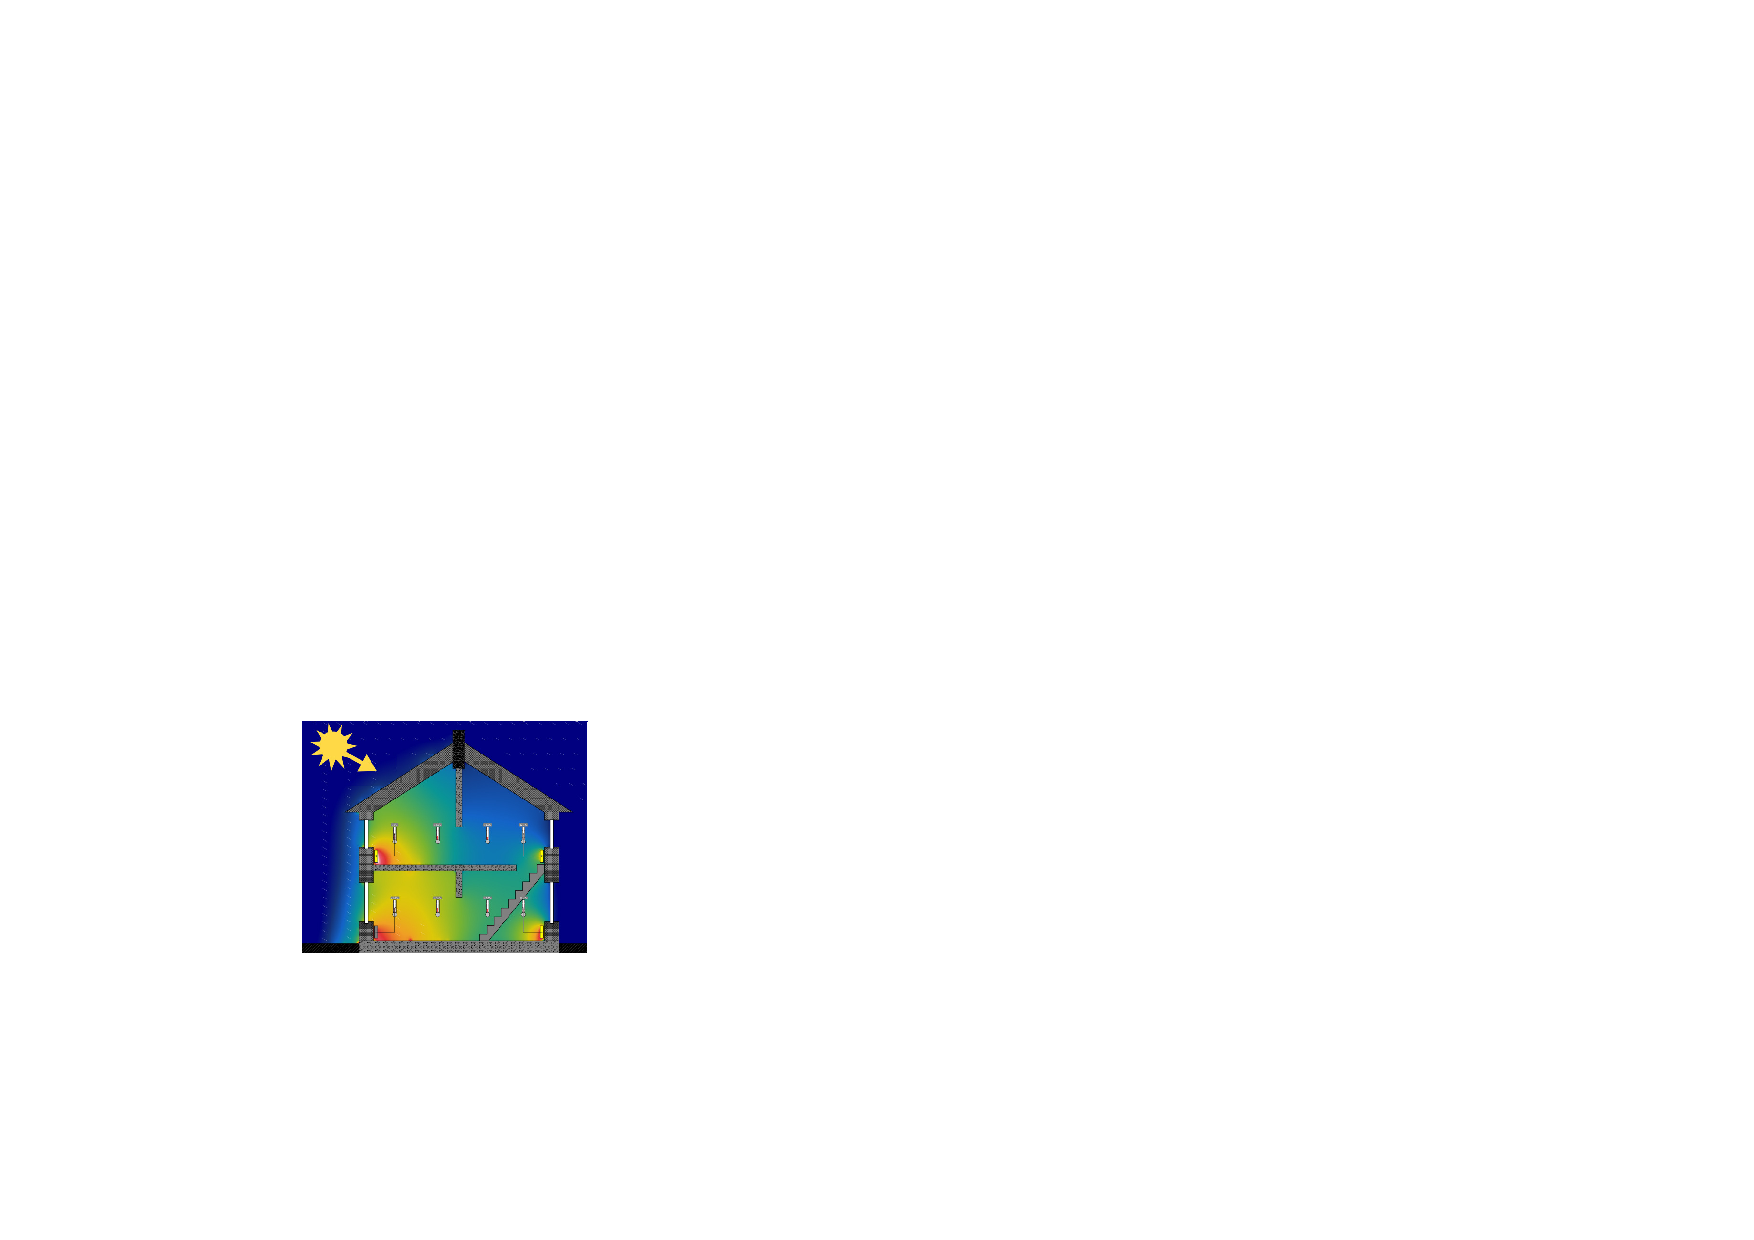
\includegraphics[width=\textwidth]{house-heating/even_powers.pdf}
		\caption{Radiator powers set evenly}
	\end{subfigure}
	~~~~ %\hspace{40pt}
		\begin{subfigure}[t]{0.47\textwidth}
			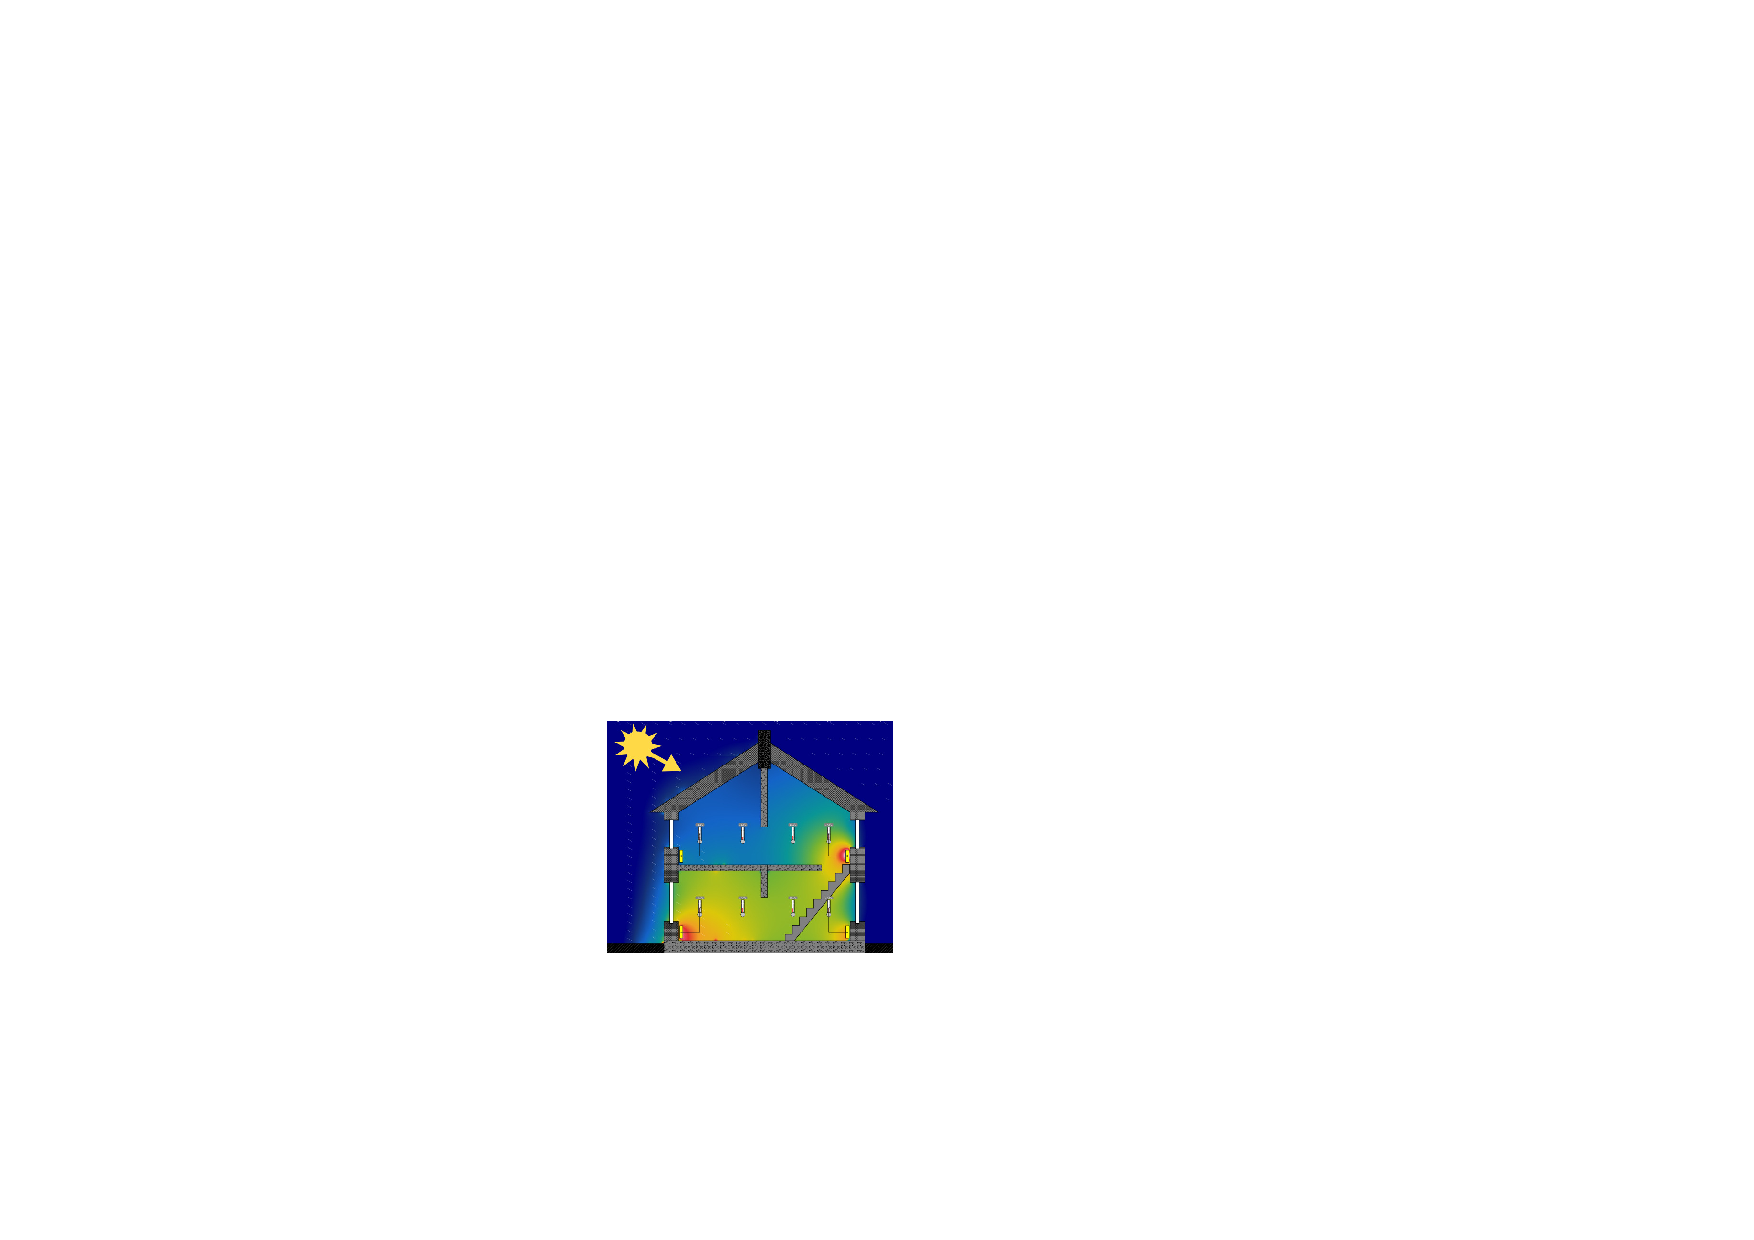
\includegraphics[width=\textwidth]{house-heating/first_iter.pdf}
			\caption{Best setup from BOPP initialization}
		\end{subfigure} \\
		\vspace{10pt}
			\begin{subfigure}[t]{0.47\textwidth}
				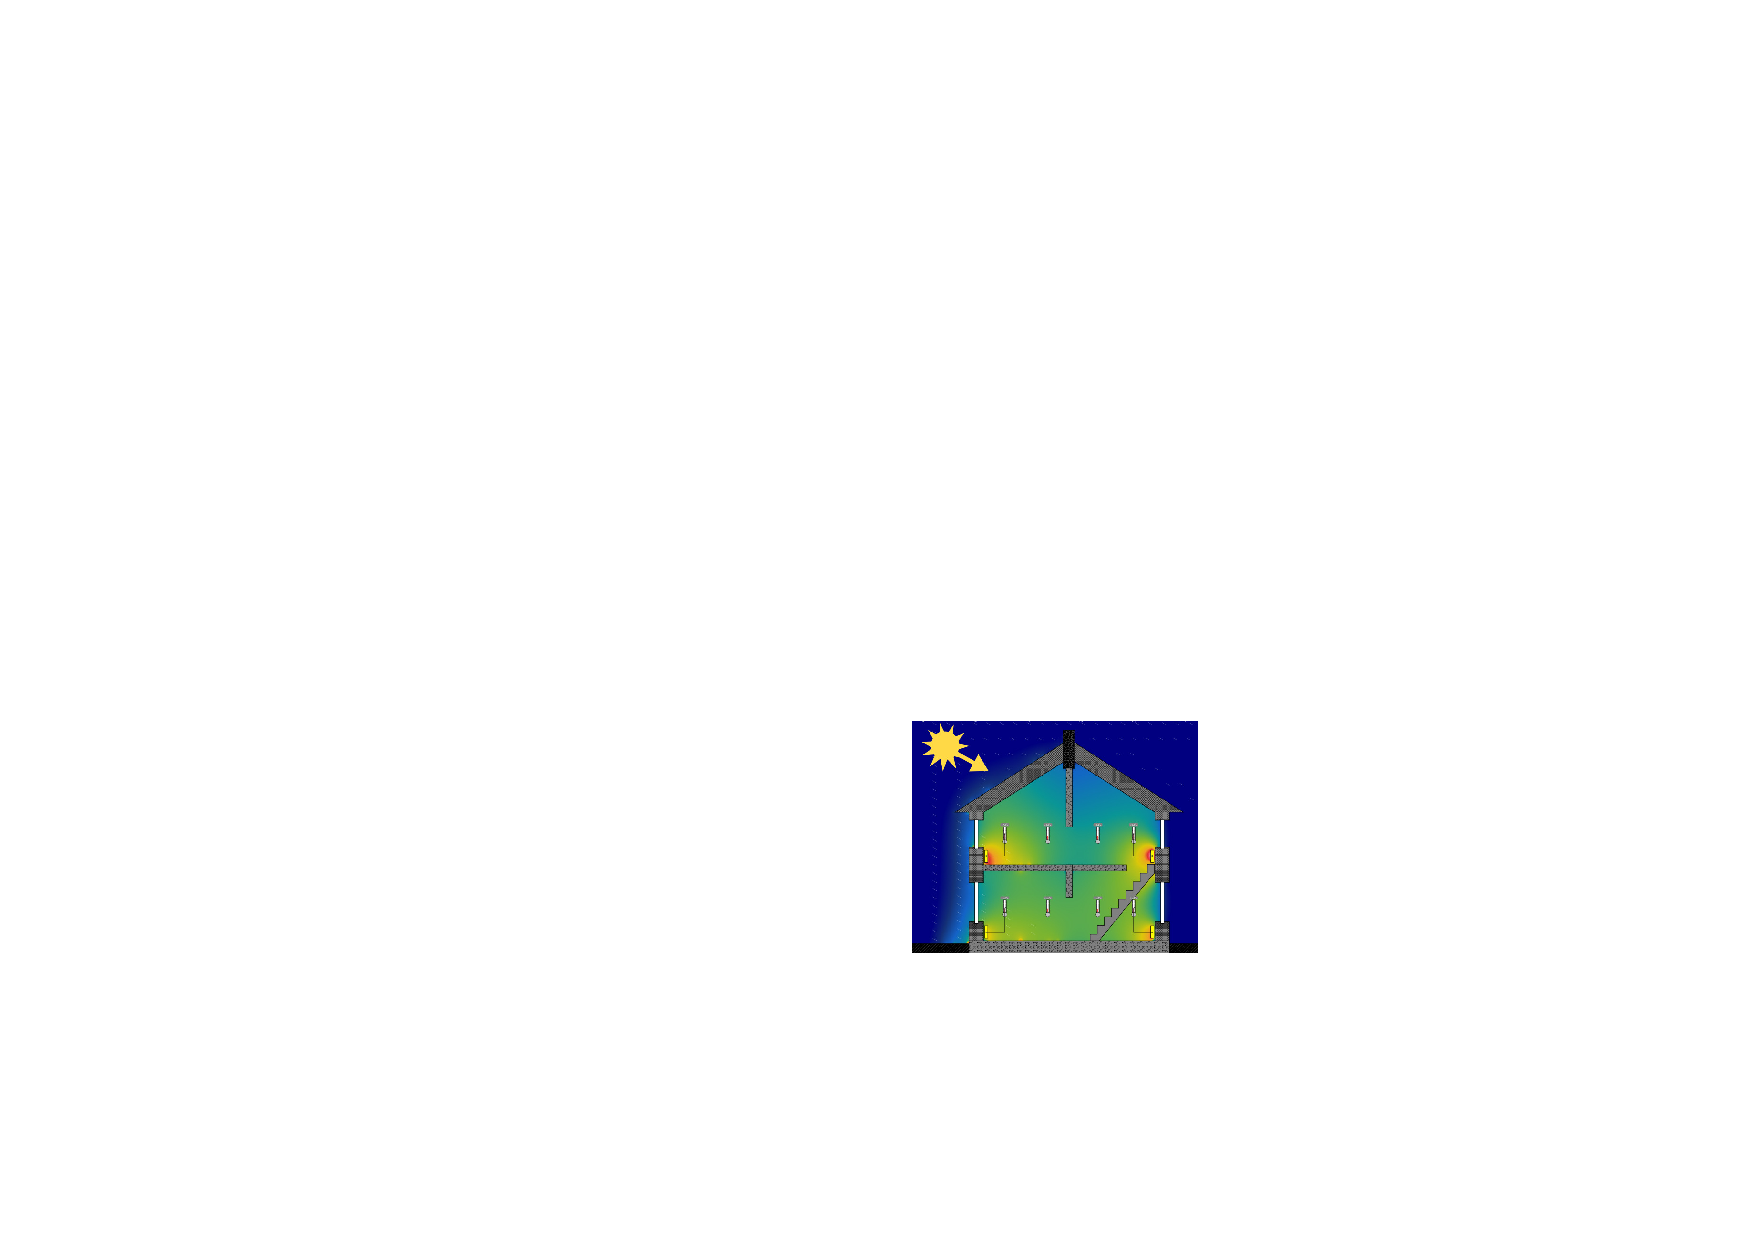
\includegraphics[width=\textwidth]{house-heating/100_iters.pdf}
				\caption{Best setup after 100 iterations of BOPP}
			\end{subfigure}
		~~~~ %	\hspace{40pt}
			\begin{subfigure}[t]{0.47\textwidth}
				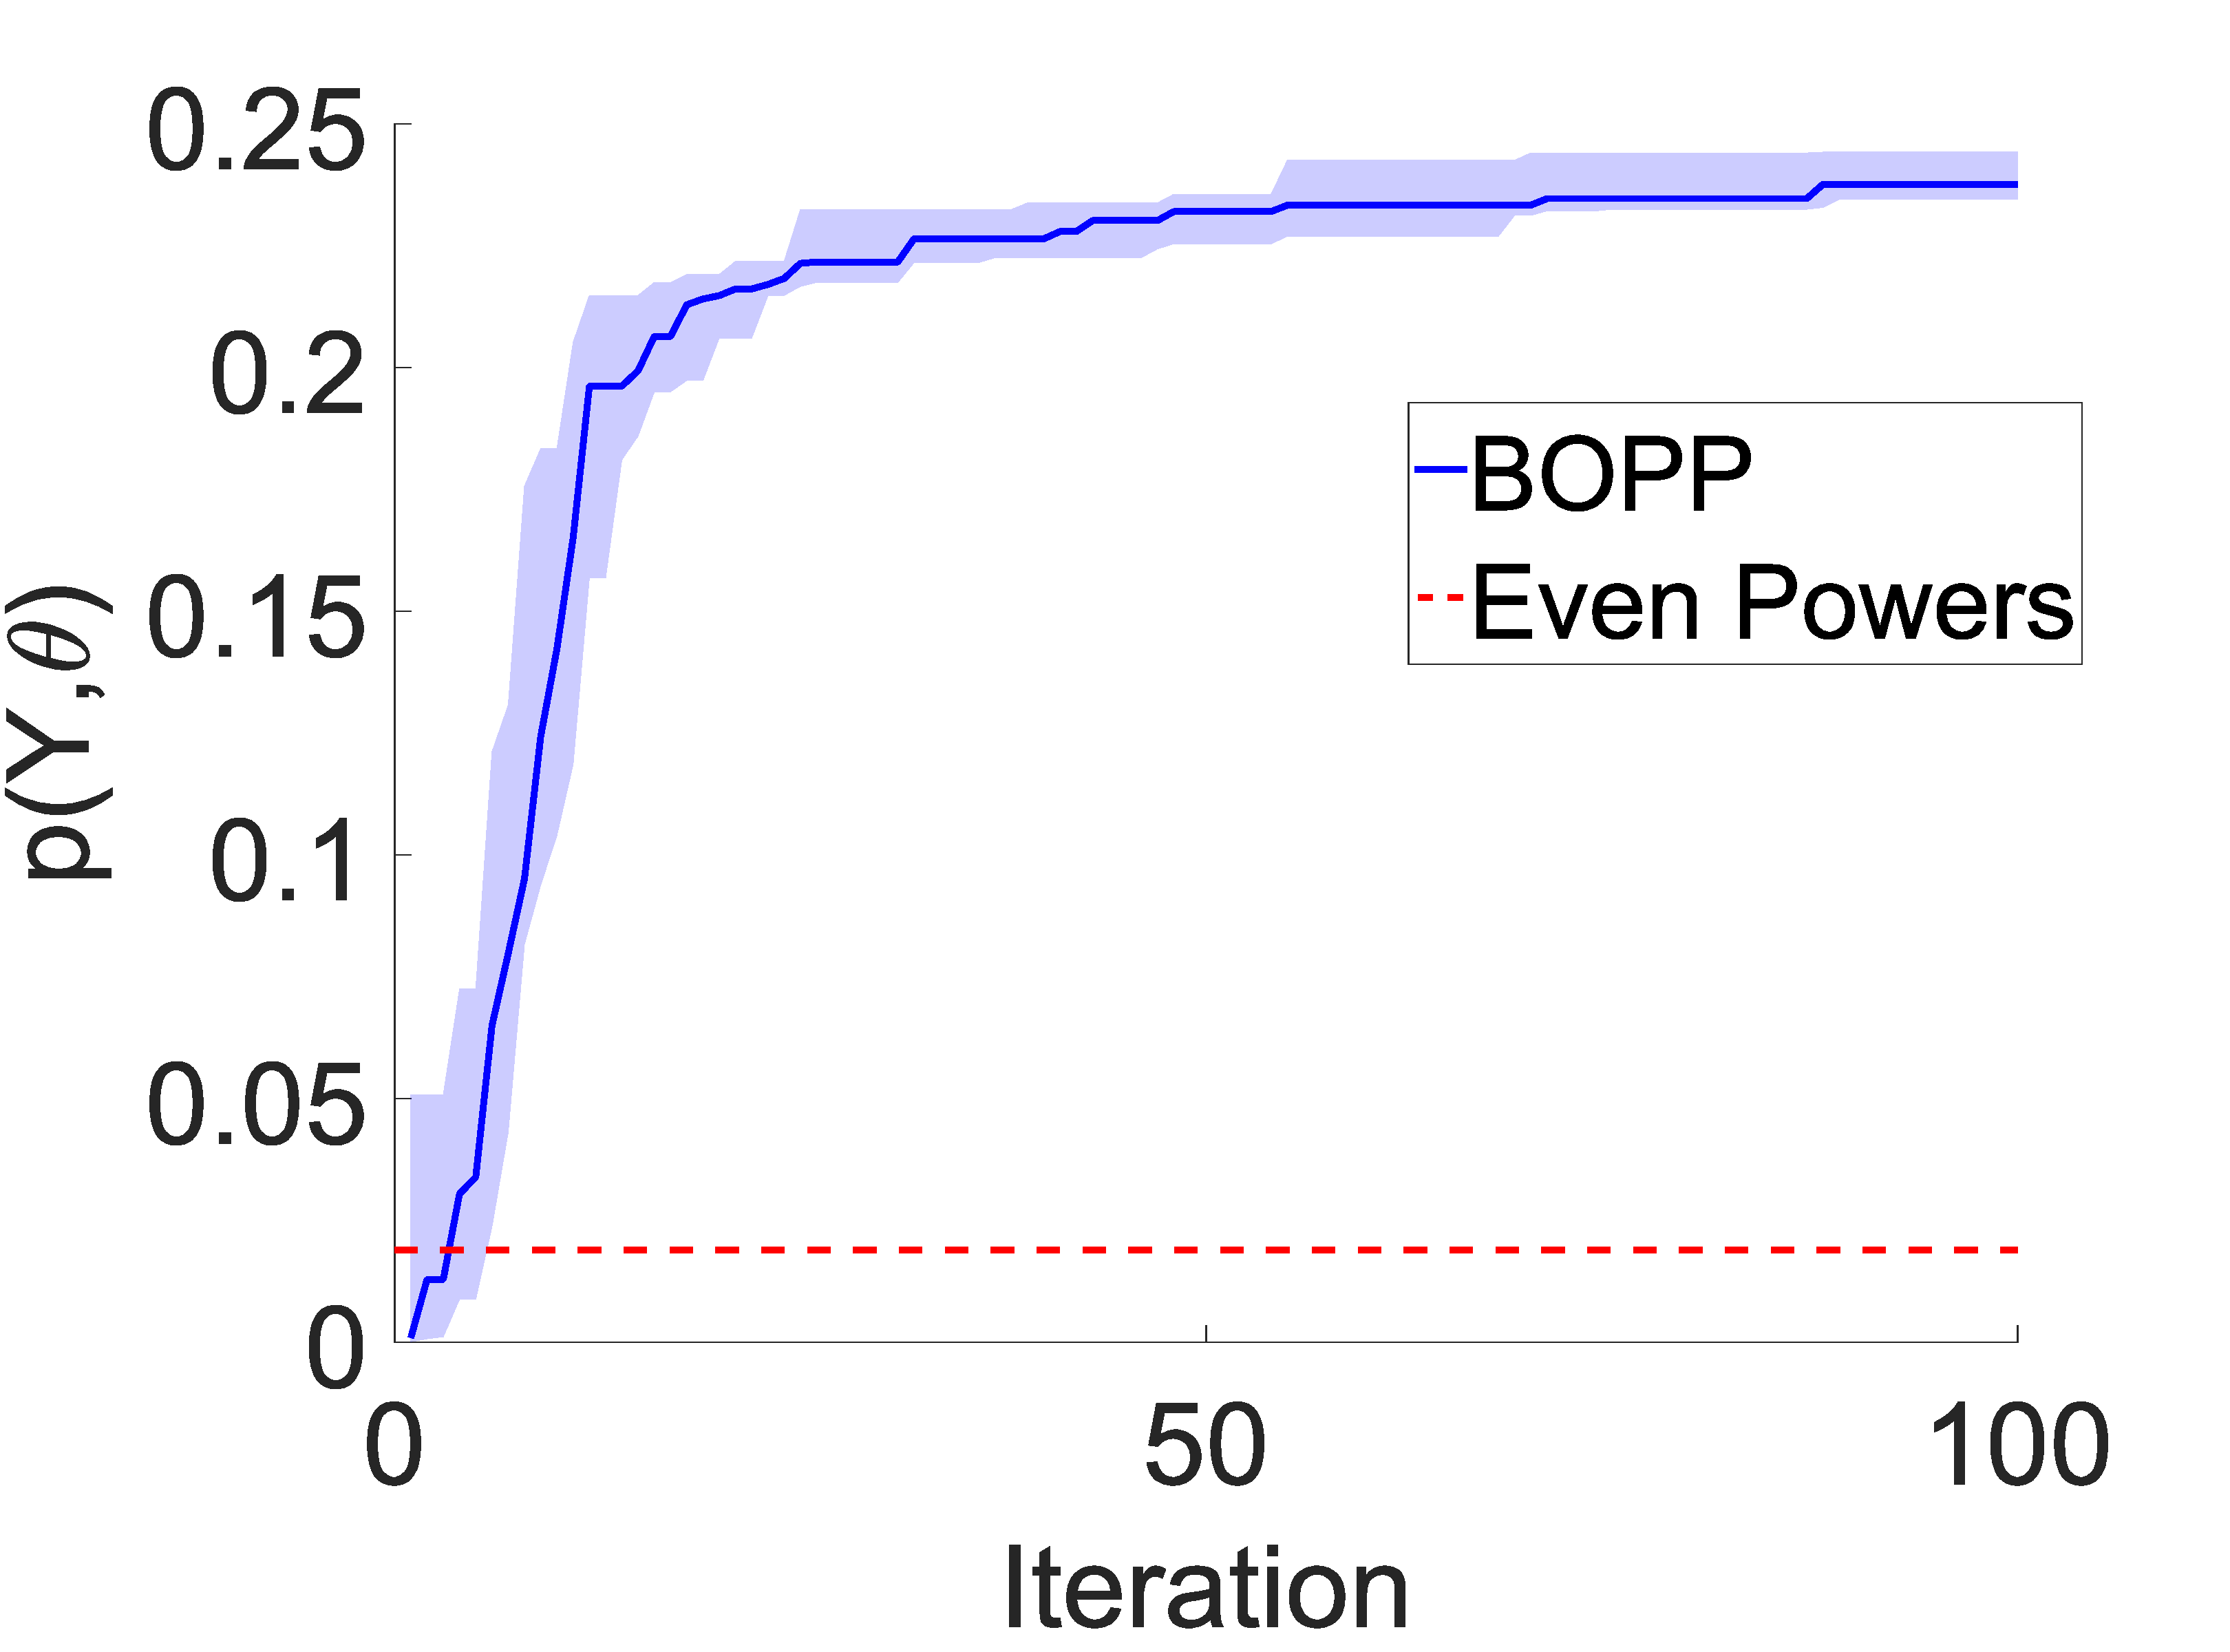
\includegraphics[width=\textwidth]{house-heating/heating_rerun.pdf}
				\caption{Convergence of evidence}
			\end{subfigure}
	% \centering ~~~
	% \includegraphics[width=0.24\textwidth]{"figures/house-heating/probabilistic/logZ-with-even-redblue-wide"}
	%			\caption{
	%				\label{fig:houses-convergence}
	%				Log marginal likelihood $\log Z$ for the \lsi{house-heating} query in Figure~\ref{fig:house-heating-code}. 
	%			}
	%	
	\caption{
		\label{fig:houses}
		Simulation-based optimization of radiator powers subject to varying solar intensity. Shown are output heat maps from Energy2D \citep{xie2012energy2d} simulations at one intensity, corresponding to setting all the radiators to the same power (\emph{top left}), the best result from a set of 5 randomly chosen powers used for initializing BOPP (\emph{top right}), and the best setup found after 100 iterations of BOPP (\emph{bottom left}). The bottom right plot shows convergence of the evidence of the respective model, giving the median and 25/75\% quartiles.
		%Simulation-based optimization of the radiator power subject to varying solar intensity. Here (a-c) show output heat maps from Energy2D \citep{xie2012energy2d} simulations, corresponding respectively to setting all the radiators to the same power, the best result from a set of randomly chosen initializations and the best setup found after 100 iterations of BOPP. (d) shows convergence of the evidence of the respective model as a function of simulation evaluations for independent restarts.
		%Homogenizing the temperature of a 2D model of a house using BOPP. The house has four adaptively controlled radiators, with additional uneven eating is provided by the sun, which will vary both temporally and probabilistically.  Our aim is to select the base power for each of the radiators, subject to some total energy budget, whilst marginalizing out the different anticipated weather conditions.  To do this, the BOPP query given in Figure \ref{fig:house-heating-code} wraps around the finite element heat transfer simulation engine Energy2D \citep{xie2012energy2d} and performs the required MMAP estimation. The na\"ive strategy of setting the power densities of the radiators uniformly (\emph{far left}) leads to an uneven heating\protect\footnotemark, noting that the colormap on the top indicates temperature of air from $5^{\circ}\mathrm C$ to $35^{\circ}\mathrm C$.  
		%After a single iteration of BOPP (\emph{middle left}), the found solution is also poor, but after 100 iterations (\emph{middle right}), a significantly improved solution has been achieved.  The log marginal likelihood in terms of iterations of number of heating setups tested is shown (\emph{far right}) for five separate BOPP runs, along with the resulting marginal likelihood from na\"ively setting the radiators to the same power.
		%Imagine that we have a number of rooms each containing a heating element and we wish to optimize the relative powers of the heaters to deliver the most uniform heating of the house over its lifetime given some total energy budget.  
		% For example, the sun will apply uneven heating to house in a manner which various over time, e.g. due to weather changes and variations in the arc of the sun through the year.  BOPP provides a basis to naturally incorporate these uncertainties into the model, whilst still exploiting the original finite element simulation and returning a single solution the engineer can the go implement.  We therefore believe that in the long term, PPS supporting MMAP have the potential to revolutionise the manner in which engineering simulation is approached by incorporating uncertainty from all stages of the process into a single unified framework, reducing the reliance on fudge-factors and educated guesswork.
	}
\end{figure*}

\begin{figure}[tb]
	\begin{lstlisting}[basicstyle=\ttfamily\small]
(defopt house-heating [alphas target-temperatures] [powers]
 (let [solar-intensity (sample weather-prior)
       powers (sample (dirichlet alphas))
       temperatures (simulate solar-intensity powers)]
  (observe (abc-likelihood temperatures) target-temperatures)))
	\end{lstlisting}	
	\vspace{-6pt}
	\caption{BOPP query for optimizing the power allocation to radiators in a house.  Here \lstinline{weather-prior} is a distribution over the solar intensity and a uniform Dirichlet prior with concentration \lsi{alpha} is placed over the powers. Calling \simulatec performs an Energy2D simulation of house temperatures. The utility of the resulting output is incorporated using \abcl, which measures a discrepency from the \texttt{target-temperatures}. Calling \doopt on this query invokes the BOPP algorithm to perform MMAP estimation, where the second input \lstinline{powers} indicates the variable to be optimized. \label{fig:house-heating-code}}
\end{figure}

Figure~\ref{fig:houses} illustrates how BOPP can be applied to engineering design, taking the example of optimizing the distribution of power between radiators in a house so as to homogenize the temperature, while marginalizing out possible weather conditions and subject to a total energy budget. The probabilistic program shown in Figure~\ref{fig:house-heating-code} allows us to define a prior over the uncertain weather, while conditioning on the output of a deterministic simulator (here Energy2D \citep{xie2012energy2d}-a finite element package for heat transfer) using an ABC likelihood.  BOPP now allows the required coincident inference and optimization to be carried out automatically, directly returning increasingly optimal configurations. 

BO is an attractive choice for the required optimization in MMAP as it is typically efficient in the number of target evaluations, operates on non-differentiable targets, and incorporates noise in the target function evaluations.  However, applying BO to probabilistic programs presents challenges, such as the need to give robust performance on a wide range of problems with varying scaling and potentially unbounded support.  Furthermore, the target program may contain unknown constraints, implicitly defined by the generative model, and variables whose type is unknown (i.e. they may be continuous or discrete).

On the other hand, the availability of the target source code in a PPS presents opportunities to overcome these issues and go beyond what can be done with existing BO packages.  BOPP exploits the source code in a number of ways, such as optimizing the acquisition function using the original generative model to ensure the solution satisfies the implicit constaints, performing adaptive domain scaling to ensure that GP kernel hyperparameters can be set according to problem-independent hyperpriors, and defining an adaptive non-stationary mean function to support unbounded BO. 

Together, these innovations mean that BOPP can be run in a manner that is fully black-box from the user's perspective, requiring only the identification of the target variables relative to current syntax for operating on arbitrary programs. We further show that BOPP is competitive with existing BO engines for direct optimization on common benchmarks problems that do not require marginalization.

%that can be implemented in any PPS where inference methods return marginal likelihood estimates. 



%MMAP estimation is generally difficult as it corresponds to the optimization of an intractable integral, such that function evaluations are expensive and give noisy results.  Current PPS inference engines are typically unsuited to such optimization.  We therefore introduce BOPP (Bayesian optimization for probabilistic programs) which couples existing inference algorithms with a new Gaussian process (GP) \citep{rasmussen2006gaussian} based Bayesian optimization (BO) \citep{osborne2009gaussian, jones1998efficient} package integrated into the PPS Anglican \citep{wood2014new}.  



%MMAP estimation for PPS presents further issues such as the need to be general purpose and robust, whilst dealing with potentially unknown constraints defined implicitly within the generative model.  


%On the other hand, the availability of the target source code in PPS presents opportunities to overcome these issues and go beyond what can be done with existing BO packages.  For example, it allows operation under unknown \emph{equality} constraints and applies automatic domain scaling for problem-independent GP hyperpriors.  In addition to delivering improved performance over prominent BO packages when used simply as an optimizer, these innovations mean that BOPP can be run in a manner that is fully black-box from the user's perspective, requiring only the identification of the target variables relative to current syntax for operating on arbitrary programs.

%\footnotetext{Though results are from the full BOPP implementation with sun heating marginalized out, the simulation plots correspond to a single common condition for the sun for visualization purposes.}

%\section{Motivating Example}
%\label{sec:motivation}


%The rest of this paper is outlined as follows: we first provide background on PPS, BO and GPs.  We define a framework for an optimization query and introduce our core code transformation to allow an arbitrary program to be optimized with respect to parameters defined within the program.  Our algorithm for optimizing the evidence of this program using BO and additional code transformations is outlined, we present experiments demonstrating the applicability of our method and we finish with concluding discussions and suggestions for future work.


\section{Related Work} 
\label{sec:bopp:related}

Reasonable consideration has been given before to solving maximum likelihood and marginal 
a posteriori (MAP) problems with PPSs and many systems provide some form of appropriate
estimation scheme (see e.g.~\citep{goodman_book_2014,carpenter2015stan,salvatier2016probabilistic}).  One simple
approach is to apply an annealing to the \observe densities (for maximum likelihood estimation)
or both the \sample and \observe densities (for MAP estimation) in
a conventional MCMC sampler such as LMH (see Section~\ref{sec:proginf:str:lmh}).
This results in a simulated annealing algorithm~\citep{aarts1988simulated} for general purpose programs.
An alternative approach, introduced by~\cite{tolpin-socs-2015}
instead uses ideas from Monte Carlo tree search to construct a general purpose MAP estimator.
However, all of these approaches do not permit the more challenging scenario
where the target is to optimize a marginal distribution.  They are, therefore, not suitable for combined
inference and optimization problems.

One approach that does consider optimization of marginal probabilities of probabilistic
programs is given by~\cite{vandemeent2016black}, which thus perhaps presents the closest
approach to our own work.  The aim of~\cite{vandemeent2016black} is, on the surface, somewhat
different to our own as they look to automate policy search problems~\citep{deisenroth2013survey}
using probabilistic programs.  However, policy search is a particular instance of MML estimation
and so falls within our general problem class.  Moreover, their approach of maximizing an evidence lower bound~\citep{blei2016variational}
using stochastic gradient ascent~\citep{robbins1951stochastic} is, in principle, substantially
more general than policy search problems and constitutes a general MML estimation scheme in its own right.
However, the approach has a number of restrictions and assumptions.  
Perhaps the most critical for our purposes is that gradients are estimated using
importance sampling and thus will generally become increasingly noisy as the dimensionality of the nuisance variables (i.e. those we wish to marginalize over) increases.
The approach also requires mean field approximations
to be made, the appropriateness of which will vary from problem to problem, while, as with other
stochastic gradient ascent approaches, a large number of optimization iterations is typically required
to reach convergence, which can be prohibitive for some problems.  BOPP, on the other hand, requires
very few assumptions to be made and is free to use more advanced inference approaches, for example
SMC, for estimating the marginal likelihood.  One consequence of this is that it can scale to far
higher dimensions in the nuisance variables.  For example, our HMM model in Section~\ref{sec:bopp:exp}
marginalizes over a roughly $5000$ dimensional space.

Another interesting alternative approach,
developed since publication of BOPP, involves taking derivatives \emph{through} an SMC
sweep~\citep{le2017auto,naesseth2017variational,maddison2017filtering}. 
More precisely, these methods allow the derivative of the marginal likelihood estimate (or more typically
its logarithm) to be calculated during an SMC sweep, for example by using automatic differentiation
on the calculation of the original estimate~\citep{le2017auto}.  This can be used for MML or MMAP estimation
of global parameters by using these gradients as input to a stochastic gradient ascent scheme.
A key difference of this approach, to say~\cite{vandemeent2016black}, is that using SMC instead of importance
sampling means that substantially lower variance gradient estimates can be achieved.
Though, to the best of our knowledge, no such approach is currently implemented in a PPS, doing so is 
in theory perfectly possible given a system supporting automatic differentiation.  
In~\cite{le2017auto}, we also show how this approach can be extended to perform simultaneous model
learning and proposal adaptation and further to an amortized inference setting, whereby we learn an inference
artifact that returns a proposal at run time.  This means that, when the model of interest comprises of
a deep neural network, then the method can be viewed as extending so-called auto-encoding methods~\citep{kingma2014auto,burda2015importance}
from their limited importance sampling setting, to a more powerful SMC framework.

\section{Problem Formulation}
\label{sec:problem}

% !TEX root =  ../main.tex

As we explained in Section~\ref{sec:probprog:models:general}, probabilistic program queries
define unnormalized distributions $\gamma(x_{1:n_x},\lambda)$ on program traces
 as defined in~\eqref{eq:probprog:universal-cond}.
At a high level, our aim is to optimize with respect to some of the $x_{1:n_x}$ variables while marginalizing out
the rest, as per MMAP estimation, MML estimation, and risk minimization introduced in
Section~\ref{sec:opt:intro}.
However, formalizing what we mean by ``some variables'' is less trivial than it would
first appear and will require specialist syntax for specifying models.  To this end,
we introduce a new query macro \defopt.  The syntax of \defopt is identical to \defquery except 
that it has an additional input identifying the variables to be optimized.  As we will
explain later, \defopt invokes a series of code transformations to produce a number
of different Anglican queries used by BOPP.  Each of these are compiled using \query
and returned as a hash map of CPS Clojure functions that can then
be used by the BOPP back end.

A possible na\"{i}ve strategy for identifying the target variables
would be to simply predefine some subset of the \sample indices
$c \subset \mathbb{N}^+$ and optimize for $\{x_j \}_{j\in c}$.  However, this is clearly not satisfactory
because it is generally an awkward method of identifying the target variables and the variables we wish
to optimize may not always be sampled at the same position in our trace (i.e. we do not want superfluous
\sample statements to effect which variables constitute our target variables).
Unfortunately though, the more natural choice of specifying any variable in the program, including those
which are deterministic functions of other variables, is not possible in general, because of complications
originating from changes of variables, namely that nonlinear deterministic mappings change the density
function in ways that it might not be possible to track.  Instead, we will still specify our target variables
$\theta = \phi_{1:L}$ by name (i.e. using the lexical name of the variable as bound by a \clj{let} block in
the raw program code), but we will place some restrictions, enforced at run time (see~\cite{rainforth2016nips}), 
to ensure validity of the model.  First, each optimization variable $\phi_{\ell}$ must be bound to a value directly 
by a \sample statement to avoid change of variable complications.
%Specifically if $\psi = g(\theta)$ then $p(Y,\theta) = \text{\bf D}_g(\psi) p(Y,\psi)$ where $\text{\bf D}_g$ represents the Jacobian associated with $g$, giving different maxima for $\theta$ and $\psi$ \cite{murphy2012machine}.
Second, in order for the optimization to be well defined, the program must be written such that any 
possible execution trace binds each optimization variable $\phi_{\ell}$ exactly once.  By proxy, this also
ensures that the number of variables to be optimized, $L$, remains fixed.
% HOW DO WE ENFORCE THIS? 
Finally, although any $\phi_{\ell}$ may be lexically multiply bound, it must have the same reference 
measure in all possible execution traces, because, for instance, if the reference measure of 
a $\phi_{\ell}$ were to change between Lebesgue to counting, the notion of optimality would 
no longer admit a conventional interpretation.  Note that we impose no restrictions on the latent
variables which will be marginalized over.

From a developer's perspective, these minor restrictions mean that all \sample statements are
either associated with a particular target variable $\phi_{\ell}$ or never associated with any target 
variable. Further, \sample
statements associated with the target variables will never be evaluated more than once (but might never
be evaluated if there are multiple possible \sample statements associated with a particular $\phi_{\ell}$) and
the total number of \sample statements associated with the target variables is always $L$.
Therefore building on the notation from Section~\ref{sec:probprog:models:general}, we will redefine $x_{1:n_x}$
as the variables that are to be marginalized over, with all associated terms similarly redefined (except $\gamma$).
We next denote the $m_{\ell}$ lexical \sample statements associated with $\phi_{\ell}$ as 
$h_{\ell,1},\dots,h_{\ell,m_{\ell}}$ with associated density functions $h_{\ell,i}(\phi_{\ell} | \xi_{\ell})$ where
$\xi_{\ell}$ is the provided distribution object (which can be a random variable but its reference measure
must be deterministic).  We further denote $c_{\ell} \in \{1,\dots,m_{\ell}\}, \; 
\forall \ell \in \{1,\dots,L\}$ as the (potentially random) variable used to index which lexical \sample statement
$\phi_{\ell}$ is drawn from in a particular execution.  We now have that the conditional distribution on the trace $\mT$ implied
by the query is $p(\mT = \{\phi_{1:L},x_{1:n_x}\} | \lambda) \propto \gamma(\theta,x_{1:n_x}, \lambda)$
where
\begin{align}
\label{eq:bopp:joint}
\gamma(\theta,x_{1:n_x}, \lambda) = \begin{cases}
\prod_{\ell=1}^{L}
h_{\ell,c_{\ell}} (\phi_{\ell} | \xi_{\ell})
\prod_{j=1}^{n_x} 
f_{a_j}(x_j | \eta_j)
\prod_{k=1}^{n_y}
g_{b_k}(y_k | \psi_k) \;\;\; \text{if} \;\;\; \mathcal{B}(\theta,x_{1:n_x},\lambda)=1 \\
0 \quad \text{otherwise}
\end{cases}
\end{align}
and we have redefined the trace validity function $\mathcal{B}(\phi_{1:L},x_{1:n_x},\lambda)$ appropriately.
As before, although many of the terms in our trace probability are random variables, all are deterministic
functions of $\{\phi_{1:L},x_{1:n_x}\}$.  Note that the relative ordering of the $\phi_{1:L}$ to the $x_{1:n_x}$
does not affect the validity of the trace or the probability, as the \sample statements associated with
each are mutually exclusive.

We can now use~\eqref{eq:bopp:joint} to define the MMAP estimate targeted by a \defopt query as
\begin{align}
\label{eq:bopp:mmap}
\begin{split}
\theta^*& (\lambda) = \argmax_{\theta \in \vartheta (\lambda)} 
\E \left[p(\mT = \{\phi_{1:L},x_{1:n_x}\} | \lambda) \middle| \theta \right]
= \argmax_{\theta \in \vartheta (\lambda)} 
\E \left[\gamma(\theta,x_{1:n_x}, \lambda) \middle| \theta \right] \\
& = \argmax_{\theta \in \vartheta (\lambda)} 
\int_{x_{1:n_x} \in \{X : \mathcal{B}(\theta,X,\lambda)=1\}} 
\prod_{\ell=1}^{L} h_{\ell,c_{\ell}} (\phi_{\ell} | \xi_{\ell})
\prod_{j=1}^{n_x} f_{a_j}(x_j | \eta_j) \prod_{k=1}^{n_y} g_{b_k}(y_k | \psi_k) dx_{1:n_x}
\end{split}
\end{align}
where $\vartheta (\lambda) := \{\theta : \exists x_{1:n_x} : \gamma(\theta,x_{1:n_x},\lambda)>0\}$
is the support of $\theta$ given $\lambda$.  
For simplicity and notational consistency with our original paper~\citep{rainforth2016nips}, 
we will now drop the dependency on $\lambda$ in the rest of the paper and instead
use the notation for MMAP estimation of a graphical model given in~\eqref{eq:opt:MMAP}
(such that we express the MMAP problem as $\theta^* = \argmax_{\theta \in \vartheta}
p(Y,\theta)$),
where $Y$ represents data and $X$ are variables marginalized over, noting that this
is not always completely accurate as per Section~\ref{sec:probprog:models:general} and 
\eqref{eq:bopp:mmap}.

To carry out the interleaving of inference and optimization required in MMAP estimation, we
introduce \doopt, which, analogous to \doquery, takes a compiled output from \defopt and
returns a lazy sequence $\{\hat{\theta}^*_m,\hat{\Omega}^*_m,\hat{u}^*_m\}_{m=1,\dots}$
where $\hat{\Omega}^*_m \subseteq X$ are the program outputs associated with
$\theta=\hth^*_m$ and each $\hat{u}^*_m \in \real^+$ is an estimate of the corresponding
log partition function $\log p(Y, \hth_m^*)$ (see Section \ref{sec:bopp-for-ml}).  The
sequence is
defined such that, at any time, $\hat{\theta}^*_m$ corresponds to the point expected to be
most optimal of those evaluated so far and allows both inference and optimization to be
carried out online.


\section{Bayesian Program Optimization}
\label{sec:bopp}

% !TEX root =  ../main.tex

On top of the syntax introduced in the previous section, there are five main components to BOPP:
\vspace{-5pt}
\begin{itemize}
	\setlength\itemsep{-0.2em}
	\item[-] A program transformation, \clj{q}$\rightarrow$\qmarg, allowing estimation of the partition function $p(Y,\theta)$ at a fixed $\theta$.
	\item[-] A bespoke, GP based, BO implementation for actively sampling $\theta$.
	\item[-] A program transformation, \clj{q}$\rightarrow$\qprior,  used for automatic and adaptive domain scaling, such that a problem-independent hyperprior can be placed over the GP hyperparameters.
	\item[-] An adaptive non-stationary mean function to support unbounded optimization.
	\item[-] A program transformation, \clj{q}$\rightarrow$\qacq, and maximum likelihood estimation method to optimize the acquisition function subject the implicit constraints imposed by query.
\end{itemize}
\vspace{-5pt}
Together these allow BOPP to perform online MMAP estimation for arbitrary programs in a manner that is black-box from the user's perspective -- requiring only the definition of the target program in the same way as existing PPS and identifying which variables to optimize.  The BO component of BOPP is both probabilistic programming and language independent, and is provided as a stand-alone package.  It requires as input only a target function, a sampler to establish rough input scaling, and a problem specific optimizer for the acquisition function that imposes the problem constraints.  %We first provide a high-level overview of the algorithm before separately explaining these components.

%BOPP provides online MMAP estimation for arbitrary programs in a manner that is black-box from the user's perspective - requiring only the definition of the target program in the same way as existing PPS and identifying which variables to optimize. It has three main components: a series of program transformations, inference schemes for evaluating these transformed programs, and a BO scheme that uses them to provide the required MMAP estimation.  Implementation of the transformations is naturally language specific, but the required techniques can be applied to any system with general-purpose languages for model specification and which provides the required inference schemes.  Given functions for evaluating these transformed programs, the BO scheme for MMAP estimation can be abstracted from probabilistic programming and is provided as its own separate package\footnote{\url{http:\\www.bitbucket.org\twgr\bo-mapp}}.  This package requires three things: a target function which provides estimates of the marginal $p(Y,\theta)$, a sampler for cheaply generating a rough representation of the input scaling, and an optimizer for the acquisition function that imposes the constraints of the problem.

\begin{figure}[t]
	\centering
	\includegraphics[width=\textwidth]{"bopp_overview_figure"}
	%\vspace{20pt}
	\caption{
		\label{fig:bopp_overview}
		Overview of the BOPP algorithm, description given in main text. \clj{p-a}, \lsi{p-}$\theta$, \lsi{p-b} and \lsi{lik} all represent distribution object constructors.
		\lsi{observe<-} is identical to \lsi{observe} except it returns the observation. \lsi{factor} is a special distribution constructor that here factors the trace probability by $\zeta(\theta)$. }
\end{figure}

Figure \ref{fig:bopp_overview} provides a high level overview of the algorithm invoked when \doopt is called on a query \clj{q} that defines a distribution $p\left(Y, a, \theta , b\right)$.  We wish to optimize $\theta$ whilst marginalizing out $a$ and $b$, as indicated by the the second input to \clj{q}. In summary, BOPP performs iterative optimization in 5 steps
\begin{description}[align=left]
	\setlength\itemsep{-0.1em}
	\item[Step 1] (\emph{blue arrows}) generates exact samples from the prior program \clj{q-prior} (\emph{top center}), constructed by removing all conditioning. This initializes the domain scaling for $\theta$.
	\item[Step 2] (\emph{red arrows}) evaluates the marginal $p(Y,\theta)$ at a small number of the generated $\hth$ by performing inference on the marginal program \qmarg~ (\emph{middle center}), which returns samples from the distribution $p\left(a,b | Y, \theta\right)$ along with an estimate of $\log p(Y, \theta)$.  The evaluated points (\emph{middle right}) provide an initial domain scaling of the outputs and starting points for the BO surrogate.
	\item[Step 3] (\emph{black arrow}) fits a mixture of GPs posterior
	to the scaled data (\emph{bottom centre}) using a problem independent hyperprior. The solid blue line and shaded area show the posterior mean and $\pm2$ standard deviations respectively. The new estimate of the optimum $\hth^*$ is the value for which the mean estimate is largest, with $\hat{u}^*$ equal to the corresponding mean.    
	\item[Step 4] (\emph{purple arrows}) constructs an acquisition function $\zeta \colon \vartheta \rightarrow \real^+$ (\emph{bottom left}) using the GPs.  This is optimized, giving the next point to evaluate $\hth_{\mathrm{next}}$, using simulated annealing on a transformed program \clj{q-acq} (\emph{middle left}) in which all \observe statements are removed and replaced with a single \observe adding a $\zeta(\theta)$ factor to the trace probability. % A non-stationary prior mean function for the GP, the AF is penalized away from a region of interest, allowing unbounded optimization.  
	%The AF is optimized by performing annealed importance sampling on a transformed program \clj{q-acq} (\emph{middle left}) in which all \observe statements are removed and replaced with a single \observe that assigns probability $\zeta(\theta)$ to the execution. 
	\item[Step 5] (\emph{green arrow}) evaluates $\hth_{\mathrm{next}}$ using \qmarg~and continues to step 3.
\end{description}

\subsection{Program Transformation to Generate the Target}
\label{sec:transform}
% !TEX root =  ../main.tex

Consider the \defopt query \texttt{q} in Figure \ref{fig:bopp_overview}, the body of which defines the joint distribution $p\left(Y,a,\theta,b\right)$.   Calculating~\eqref{eq:opt:MMAP} (defining $X=\left\{a,b\right\}$) using a standard optimization scheme presents two issues: $\theta$ is a random variable within the program rather than something we control and its probability distribution is only defined conditioned on $a$.

We deal with both these issues simultaneously using a program transformation similar to the disintegration transformation in Hakaru \citep{zinkov2016composing}. Our \emph{marginal} transformation can be thought of generating a new query, \qmarg~ as shown in Figure~\ref{fig:bopp_overview}, that defines the same unnormalized joint distribution on program variables and inputs (i.e. $\gamma(\theta,x_{1:n_x},\lambda)$ is unchanged), but now accepts the value for $\theta$ as an input (i.e. the $\phi_{1:L}$ become terms in $\lambda$ rather than being random variables).  As such, the partition function of the program is
now a function of $\theta$ and therefore can be optimized using an external algorithm.
The transformation itself replaces all \sample statements associated with each $\phi_{\ell}$ with an equivalent \observes statement, taking $\phi_{\ell}$ as the observed value, where \observes is identical to \observe except that it returns the observed value instead of \clj{nil}.  As both \sample and \observe operate on the same variable type -- a distribution object -- this transformation can always be made, while the identical returns of \sample and \observes trivially ensures validity of the transformed program.  The transformation used for MML and risk
minimization
is equivalent except that the \observe statements are replaced by an identity function (rather than \observes), such
that the transformation effectively removes the original \sample statements.

In truth, the transformations used by BOPP are not exactly as shown in~\ref{fig:bopp_overview}
and as described above.  This is because, although for simple programs, such as the given
example, these transformations can be easily expressed as static transformations, for more
complicated programs it would be difficult to actually implement these as purely static
generic transformations in a higher-order language.  Therefore, even though all the
transformations dynamically execute as shown at runtime, in truth, the generated source 
code for the prior and acquisition transformations varies from what is shown and has 
been presented this way in the interest of exposition.  Our true transformations exploit
the existing Anglican special forms \lsi{store} and \lsi{retrieve} and two new
special forms we introduce called \lsi{catch} and \lsi{throw}, in order to generate programs
that dynamically execute in the same way at run time as the static examples shown, but
whose actual source code varies significantly.  Full details are given in~\cite{rainforth2017boppArxiv}.

%We now build upon our optimization query to demonstrate how BOPP can optimize with respect to an arbitrary subset of variables sampled within a PP.  This is equivalent to optimizing with respect to an arbitrary subset of nodes in a graphical model, whilst marginalizing over the others, representing a new method beyond the scope of current BO algorithms.


%Consider the Anglican query \texttt{q} in figure \ref{fig:originalQuery} as a demonstrative example.  The marginal distribution defined by \texttt{q}, $p\left(Y,\theta\right) = \int_{U} \int_{V} p\left(U\right)p\left(\theta|U\right)p\left(V|\theta,U\right)p\left(Y|V,\theta,U\right)dUdV$, is the same objective function as in~\eqref{eq:hyperOpt} if we define $X= \left\{U,V\right\}$, but $\theta$ is no longer at the root of the dependency structure as it was in \eqref{eq:Joint}.  This causes two problems for optimizing with respect to $\theta$: it is sampled within the program and the corresponding probability distribution is only defined conditioned on one of the parameters we wish to marginalize over $U$.  

%We propose dealing with both these issues simultaneously using a program transformation by which we change any \sample statements for elements of $\theta$ into \observes statements, resulting in the transformed query \texttt{qT} shown in \ref{fig:transformedQuery}.  Here \observes is identical to \observe except that its return value is equal to its observation, in this case $\theta$.  The transformed query is a function of $\theta$ and can therefore be optimized.  When \doquery is called on \texttt{q} with the BOPP algorithm specified as the inference engine, it acts a macro which first makes this transformation before passing the transformed program to our BO wrapper.

%At a high level, the result of this transform is that we use use the defined probability distribution for sampling $\theta$ to condition the program to a particular value of $\theta$.  Critically, the distribution defined by the program has not changed.  This is easiest to assert by considering the program as defining a joint density on the sampled variables and the observations, and noting that whether these variables are fixed or sampled at runtime does not change the definition of this joint.  This simple but elegant solution means that we can transform any probabilistic program, and therefore any graphical model, to an optimization problem with respect to any of its sampled variables. 





%\subsection{Marginal Maximum A Posteriori Estimation}
%% !TEX root =  bopp.tex

%In this section we introduce a set of requirements for an ``optimization query", which returns an infinite lazy sequence of increasingly optimal estimates for some target variables $\theta \in \vartheta$.  For exposition purposes, we first consider the case where $\theta$ correspond to the inputs of a query $q$ and show how this can be extended to arbitrary variables within the program in section \ref{sec:transform}. We assume $q$ takes as inputs, along with $\theta$ data upon which the query is conditioned $Y$.


%As it is only possible to estimate $p(Y, \hth_m)$ such that
%\begin{align}
%\label{eq:BOPPoutput}
%E_f\left[\hat{p} \left(Y,\hth_m\right) | D_{m} \right] \ge E_f\left[\hat{p} \left(Y,\hth_j\right) | D_{m} \right] \quad \forall j=1,\dots,m-1
%\end{align}
%where $\hat{p}$ is used to indicate that the estimation of the marginal probability is itself probabilistic due to the approximation nature of inference. 

Given the above program transformation we can use a generic inference method provided by the back end to marginalize over the latent variables $X$ conditioned on $\theta$. We will here use sequential Monte Carlo for probablistic programs \citep{wood2014new} to obtain unnormalized estimates of the marginal conditional likelihood
\begin{align}
\hw \left(Y,\theta\right) \approx p\left(Y | \theta\right) =\int p\left(X,Y|\theta\right) dX.
\end{align}
Given these estimates we are now in a position to define the problem setting for MMAP estimation in probabilistic programs. Specifically we will define a macro \lsi{doopt} that accept a query defined using \lsi{defopt} and returns a lazy sequence of increasingly optimal estimates for the target variables $\theta$. We now formally define our optimization query to output an infinite lazy sequence $\{\hth_1,\hat{\Omega}_1\},\{\hth_2,\hat{\Omega}_2\},\dots$ where $\hat{\Omega}_i$ is the map of \predict values with the query when $\theta=\hth_i$ and
\begin{align}
\label{eq:BOPPoutput}
E\left[\hw \left(Y,\hth_m\right) p\left(\hth_m\right) | D_{m} \right] \ge E\left[\hw \left(Y,\hth_j\right) p\left(\hth_j\right) | D_{m} \right] \quad \forall j=1,\dots,m-1 \quad m=1,2,\dots
\end{align}
where the expectation is over the surrogate function posterior. $\hth_m$ corresponds to the point that is expected to be the most optimal of those evaluated under the posterior of our surrogate function. Since evaluations of are noisy, this need not be the $\theta$ value that produced the highest the $p(\theta)$-weighted marginal likelihood estimate. % Further as the observation of a new point affects the surrogate function posterior at all other points (as the expectation of both sides of~\eqref{eq:BOPPoutput} is conditioned on all data observed so far $D_m$), $\hth_m$ can change between different historical values when a new point is queried.


% Consider a generic query $q$.  Let the \sample statements within the $q$ define a generative distribution for a set of latent variables $X = \left\{x_{i}\right\}_{i=1,\dots,N}, \; X \in \mathcal{X}$ (note $x_i$ may have different support for different $i$) with prior $p\left(X | \theta\right) = p\left(x_1 | \theta\right) \prod_{i=2}^{N} p\left(x_i | x_1,\dots,x_{i-1},\theta\right)$, parametrized by a set of program inputs $\theta \in \vartheta$.  Let the \observe statements in the program define conditioning on observations $Y = \left\{y_i\right\}_{i=1,\dots,N}, \; Y \in \mathcal{Y}$ such that the query defines the joint factorization\footnote{Note, there is notational deficiency as in a higher-order PPS variable types, the order of the conditioning for the latent variables and even the number of latent variables can change depending on the program trace.}
% \begin{multline}
% \label{eq:Joint}
% p\left(X,Y|\theta\right) = p\left(x_1 | \theta\right) p\left(y_1 | x_1, \theta\right) \\ \prod_{i=2}^{N} p\left(y_i | x_1,\dots,x_{i},\theta\right) p\left(x_i | x_1,\dots,x_{i-1},\theta\right).
% \end{multline}
% We assume that the observations $Y$ are fixed and finite dimensional.  Our aim is to optimize the marginal likelihood of this joint scaled by a prior on $\theta$:
% \begin{align}
% \label{eq:hyperOpt}
% \theta^* = \argmax_{\theta \in \vartheta} p\left(\theta\right) \int_{X}^{} p\left(X,Y|\theta\right) dX,
% \end{align}

%Often the prior on $\theta$ will often correspond only to a set of bounds, giving a uniform distribution within the permissible input space.  If $p\left(\theta\right)$ is allowed to be potentially improper,~\eqref{eq:hyperOpt} also incorporates maximum likelihood estimation .  
%restricting the choice of inference algorithm. Anglican supports a number of suitable algorithms including importance sampling \citep{glynn1989importance}, sequential Monte Carlo (SMC) \citep{smith2013sequential,wood_aistats_2014} and the particle cascade \citep{paige2014asynchronous}.


For clarity we introduce the following notation of the rest of the paper.  We use $\theta_m$ to refer to the $\theta$ used to call the query at iteration $m$, and $\Omega_m$ and $W_m$ for the predicts and marginal likelihood estimate from this call respectively.  We define $\jsm \in \{1,\dots,m\}$ to be the index corresponding to the estimated best $\theta_m$ at iteration $m$ such that $\hth_m = \theta_{\jsm}$.  We further define $Z_m \coloneqq W (Y,\theta_j) p(\theta_j)$ and $\hz_m \coloneqq \hw (Y,\hth_j) p(\hth_j)$ as the corresponding estimates of the weighted marginal weights.

%We finally note that our optimization query includes as a special case independent calls to an inference query by setting $\ell (\cdot) = 0$ and by convention taking the most recent sample under equality of~\eqref{eq:BOPPoutput}.  Furthermore, one is free to choose the sequence of $\tilth$ in anyway desired.  For example, one may wish to explicitly control the trade off between improving our estimates for $\theta^*$, and refining the inference of the latent variables $p(z | y, \tilth_{\jsm})$ by recalling the original query with the same $\theta$.


\subsection{Bayesian Optimization of the Marginal}
\label{sec:BOPP}

% !TEX root =  ../main.tex

The target function for our BO scheme is $\log p(Y,\theta)$, noting $\argmax f\left(\theta\right) = \argmax \log f\left(\theta\right)$ for any $f : \vartheta \rightarrow \real^+$.  The log is taken because GPs have unbounded support, while $p\left(Y,\theta\right)$ is always positive, and because we expect variations over many orders of magnitude.  PPS with importance sampling based inference engines, e.g. SMC or the particle cascade (see Section~\ref{sec:proginf:str}), can return noisy estimates of this target given the transformed program \qmarg.   Full details on our BO scheme can be found
in~\cite{rainforth2017boppArxiv}, a summary of which is provided below.

Our BO scheme uses a GP prior and a Gaussian likelihood.  Though the rationale for the latter is predominantly computational, giving an analytic posterior, there are also theoretical results suggesting that this choice is appropriate \cite{berard2014lognormal}. We use as a default covariance function a combination of a Mat\'{e}rn-3/2 and Mat\'{e}rn-5/2 kernel. By using automatic domain scaling as described in the next section, problem independent priors are placed over the GP hyperparameters such as the length scales and observation noise.  Inference over hyperparameters is performed using Hamiltonian Monte Carlo (HMC) \citep{duane1987hybrid}, giving an unweighted mixture of GPs.  Each term in this mixture has an analytic distribution fully specified by its mean function $\mu_m^i \colon \vartheta \rightarrow \real$ and covariance function $k_m^i \colon \vartheta \times \vartheta \rightarrow \real$, where $m$ indexes the BO iteration and $i$ the hyperparameter sample.

This posterior is first used to estimate which of the previously evaluated $\hth_j$ is the most optimal, by taking the point with highest expected value, $\hat{u}^*_m = \max_{j\in1\dots m} \sum_{i=1}^{N} \mu_{m}^i (\hth_j)$.  This completes the definition of the output sequence returned by the \doopt macro.  Note that as the posterior updates globally with each new observation, the relative estimated optimality of previously evaluated points changes at each iteration.
Secondly it is used to define the acquisition function $\zeta$, for which we take the expected improvement \cite{snoek2012practical}, defining $\sigma_m^i\left(\theta\right) = \sqrt{k_m^i\left(\theta,\theta\right)}$ and $\gamma_m^i\left(\theta\right) = \frac{\mu_m^i \left(\theta\right)-\hat{u}_m^*}{\sigma_m^i\left(\theta\right)}$,
\begin{align}
\label{eq:exp-imp}
\zeta \left(\theta\right) = \sum_{i=1}^{N} \left(\mu_m^i\left(\theta\right)-\hat{u}_m^*\right)\Phi \left(\gamma_m^i\left(\theta\right)\right)+\sigma_m^i\left(\theta\right)\phi\left(\gamma_m^i\left(\theta\right)\right)
\end{align}
where $\phi$ and $\Phi$ represent the pdf and cdf of a unit normal distribution respectively.   We note that more powerful, but more involved, acquisition functions, e.g. \cite{hernandez2014predictive}, could be used instead.

\label{sec:bopp-for-ml}

% !TEX root =  ../main.tex

\subsection{Automatic and Adaptive Domain Scaling}
\label{sec:bopp:domain}

Domain scaling, by mapping to a common space, is crucial for BOPP to operate in the required black-box fashion as it allows a general purpose and problem independent hyperprior to be placed on the GP hyperparameters.  BOPP therefore employs an affine scaling to a $[-1,1]$ hypercube for both the inputs and outputs of the GPs.  To initialize scaling for the input variables, we sample directly from the generative model defined by the program. %\footnote{Note that Anglican's ability to include statements for conditioning on generated variables, for example to truncate distributions, means this does not always represent $p(\theta)$ and is only a prior in a more abstracted sense.}
This is achieved using a second transformed program, \qprior, which removes all conditioning, i.e. \observe statements, and returns $\theta$.  This transformation also introduces code to terminate execution of the query once all $\theta$ are sampled, in order to avoid unnecessary computation.
As \observe statements return \lsi{nil}, this transformation trivially preserves the generative model of the program, 
but the probability of the execution changes. Specifically, if we denote $n_{\theta}$ as the number of non-target \sample 
statements that have been invoked by the time all $\phi_{1:L}$ are sampled, then \qprior more formally defines the
\emph{unconditional} distribution $p_{\lambda}(\mT = \{\phi_{1:L},x_{1:n_{\theta}}\}) \propto 
\gamma_{\text{prior}}(\theta,x_{1:n_{\theta}},\lambda)$ where
\begin{align}
\label{eq:bopp:qprior}
\gamma_{\text{prior}}(\theta,x_{1:n_{\theta}},\lambda)= \begin{cases}
\prod_{\ell=1}^{L}
h_{\ell,c_{\ell}} (\phi_{\ell} | \xi_{\ell})
\prod_{j=1}^{n_{\theta}} 
f_{a_j}(x_j | \eta_j) \;\;\; \text{if} \;\;\; \mathcal{B}(\theta,x_{1:n_\theta},\lambda)=1 \\
0 \quad \text{otherwise}
\end{cases}
\end{align}
and the trace validity function $\mathcal{B}(\theta,x_{1:n_\theta},\lambda)$ is redefined appropriately.
Because~\eqref{eq:bopp:qprior} is an unconditional distribution, it can be sampled from directly by
running the program forwards, returning exact samples from the corresponding marginal distribution on $\theta$.
This is computationally inexpensive, as it does not require inference or calling potentially expensive 
likelihood functions.  It can thus be cheaply sampled from a number of times to initialize the input scaling.
By further running inference on \qmarg~given a small number of these samples as arguments, a rough initial characterization of output scaling can also be achieved and initial samples for the BO algorithm generated. 

If points are later observed that fall outside the hypercube under this initial scaling, the domain scaling 
is appropriately updated so that the target for the GP remains the $[-1,1]$ hypercube.  
An important exception to this is that the output mapping to the bottom of the hypercube remains 
fixed and any points with partition function estimates lower than this are not incorporated into the scaling in any way,
i.e. the input scaling is not updated to incorporate these points either.
For MMAP estimation, this ensures stability for unbounded problems as there can only be a finite region
of the input space where the true value of the partition function is above any given value because its integral
over $\theta$ must be finite.  Similarly, the
maximum possible estimate the inference algorithm might return will be bounded
given some weak assumptions (roughly that $p(Y,X,\theta)$ is itself bounded).
Consequently, the fixed base of the hypercube (as dictated by the initial samples) ensures that the 
there is a maximum possible size the hypercube can reach.
For risk minimization (where our target is $-\log p(Y,\theta)$) and  MML estimation
(where our target is $\log p(Y|\theta)$) problems then we have no such guarantee that the adaptation will 
eventually cease.  However, this is somewhat inherent to unbounded global optimization problems,
rather than being a specific issue of BOPP.

\subsection{Unbounded Bayesian Optimization via Non-Stationary Mean Function Adaptation}
\label{sec:bopp:unbounded}

Unlike standard BO implementations, BOPP is not provided with external constraints and we therefore 
develop a scheme for operating on targets with potentially unbounded support.  For MMAP estimation,
the target function is an unnormalized density, implying that the area that must 
be searched in practice to find the optimum is finite.  For MML estimation and risk minimization this
assumption is still reasonable in practice as if it is not true, we are effectively doomed to fail anyway.
We, therefore, exploit this assumption by defining a non-stationary prior mean function.  
This takes the form of a bump function that is constant within a region of interest, but decays rapidly 
outside.  Specifically we define this bump function in the transformed space as
\begin{align}
\label{eq:BUMP}
\mu_{\mathrm{prior}}\left(r;r_e,r_{\mathrm{\infty}}\right) = \begin{cases} 0  \hfill & \mathrm{if} \; r \leq r_{\mathrm{e}} \\ 
\log \left(\frac{r-r_{\mathrm{e}}}{r_{\mathrm{\infty}}-r_{\mathrm{e}}}\right)+\frac{r-r_{\mathrm{e}}}{r_{\mathrm{\infty}}-r_{\mathrm{e}}} & \mathrm{otherwise} \end{cases}
\end{align}
where $r$ is the radius from the origin, $r_e$ is the maximum radius of any point generated 
in the initial scaling or subsequent evaluations, and $r_{\mathrm{\infty}}$ is a parameter 
set to $1.5 r_{e}$ by default.  Consequently, the acquisition function also decays and new points 
are never suggested arbitrarily far away.  Adaptation of the scaling will automatically update this 
mean function appropriately, learning a region of interest that matches that of the true problem, 
without complicating the optimization by over-extending this region.  We note that our method 
is very similar to the independently developed work of \cite{shahriari2016unbounded}, but overcomes the 
sensitivity of their method upon a user-specified bounding box representing soft constraints, 
by initializing automatically and adapting as more data is observed.

An important consequence of this approach is that BOPP is not always an entirely
global optimizer as the adaptation can, at least in theory, become stuck around a single mode if
their is extreme prior-target mismatch.  Specifically, because only ``bad'' points 
are not incorporated into the rescaling as described in the last
section, it may be that region where the target is low blocks expansion to another mode.
In practice, such occurrences should be extremely rare (at least for MMAP estimation) as the
initial scaling is approximately set to the region where the generative model has reasonable density, such that
the problem would need to be both multi-modal and have extreme prior-target mismatch for BOPP to
get stuck.  One could in theory refine our method to provide better guarantees against such occurrences,
but given the inherent difficulty of such problems and the fact that BOPP, like other GP-based BO methods,
is heavily restricted in the number of iterations before the GP training cost becomes
prohibitive (usually in the hundreds of iterations), doing so seems more likely in practice to do harm than good.

% !TEX root =  bopp.tex

\subsection{Optimizing the Acquisition Function}
\label{sec:optacqfunc}

Optimizing the acquisition function for BOPP presents the issue that the query contains implicit constraints that are unknown to the surrogate function.  The problem of unknown constraints has been previously covered in the literature \citep{gardner2014bayesian,hernandez2015general} by assuming that constraints take the form of a black-box function which is modeled with a second surrogate function and must be evaluated in guess-and-check strategy to establish whether a point is valid. Along with the potentially significant expense such a method incurs, this approach is inappropriate for \emph{equality} constraints or when the target variables are potentially discrete.  For example, the Dirichlet distribution in Figure~\ref{fig:house-heating-code} introduces an equality constraint on \lsi{powers}, namely that its components must sum to $1$.

We therefore take an alternative approach based on directly using the program to optimize the acquisition function.  To do so we consider a transformed program \lsi{q-acq} that is identical to \lsi{q-prior} (see Section \ref{sec:domain}), but adds an additional \observe statement that assigns a weight $\zeta(\theta)$ to the execution.  By setting $\zeta(\theta)$ to the acquisition function, the maximum likelihood corresponds to the optimum of the acquisition function subject to the implicit program constraints.  %Critically, this evaluation does not require inference and so can be evaluated cheaply.
We obtain a maximum likelihood estimate for \lsi{q-acq} using a variant of annealed importance sampling \citep{neal2001annealed} in which lightweight Metropolis Hastings (LMH) \citep{wingate2011lightweight} with local random-walk moves is used as the base transition kernel. %The latter of these, which we refer to as random-walk Metropolis Hastings (RMH), is made possible by examining the type of the relevant distribution object at runtime to generate an appropriate local proposal kernel given the distribution type.

%Our final transformation generates a program, \qacq, which is identical to \qprior, except for adding an additional \observe statement that assigns a weight $\zeta(\theta)$ to the execution, where $\zeta$ is a function provided as an input.  By setting $\zeta(\theta)$ to the acquisition function and using a maximum likelihood algorithm to optimize the program, the optimum of the acquisition function subject to the implicit program constraints can be found as detailed in Section \ref{sec:optacqfunc}.
%
%\subsection{Problem Independent Gaussian Process Hyperprior}
%\label{sec:app:hyperprior}
%
%% !TEX root = bopp.tex

Remembering that the domain scaling introduced in Section~\ref{sec:domain} means that both the input and outputs of the GP are taken to vary between $\pm1$, we define the problem independent GP hyperprior as $p(\alpha)=p(\sigma_n)p(\sigma_{3/2})p(\sigma_{5/2})\prod_{i=1}^{D}p(\rho_i)p(\varrho_i)$ where
\begin{subequations}
	\begin{align}
	\label{eq:hyperPriorDef}
	\log \left(\sigma_n\right) & \sim \mathcal{N} \left(-5,2\right) \\
	\log\left(\sigma_{3/2}\right) & \sim \mathcal{N} \left(-7,0.5\right)\\
	\log\left(\sigma_{5/2}\right) & \sim \mathcal{N} \left(-0.5,0.15\right)\\
	\log \left(\rho_i\right) & \sim \mathcal{N} (-1.5,0.5) \quad \forall i \in \{1,\dots,D\}\\
	\log\left(\varrho_i\right) & \sim \mathcal{N} \left(-1,0.5\right) \quad \forall i \in \{1,\dots,D\}.
	\end{align}
\end{subequations}
The rationale of this hyperprior is that the smoother Mat\'{e}rn 5/2 kernel should be the dominant effect and model the higher length scale variations. The Mat\'{e}rn 3/2 kernel is included in case the evidence suggests that the target is less smooth than can be modelled with the Mat\'{e}rn 5/2 kernel and to provide modelling of smaller scale variations around the optimum.

\section{Experiments}
\label{sec:bopp:exp}

% !TEX root =  ../main.tex

%We evaluate our BOPP framework in two case studies that represent different use cases for Bayesian optimization. In both problem settings Bayesian optimization serves to minimize the number of evaluations needed for a computationally expensive operation. The first problem is hyperparameter optimization for probabilistic programs. Here the expensive step is marginalization over the non-optimized random variables in a program, which is performed using one of the generic inference methods provided by Anglican's inference back end. In the second case study we consider programs in which an expensive forward simulation is used to perform approximate Bayesian computation. Here the use of probabilistic programming allows determination of parameters that are marginally optimal with respect to some distribution of simulation inputs.

\begin{figure*}[t]
	%	\includegraphics[width=1.35in,trim={0 0 0 0},clip]{figures/simple-bimodal/simple-bimodal-160229-03-5.png}
	%	\includegraphics[width=1.35in]{figures/simple-bimodal/simple-bimodal-160229-03-10.png}
	%	\includegraphics[width=1.35in]{figures/simple-bimodal/simple-bimodal-160229-03-20.png}
	%	\includegraphics[width=1.35in]{figures/simple-bimodal/simple-bimodal-160229-03-50.png}
	%\includegraphics[width=1.65in]{"figures/simple-bimodal/simple-bimodal-160229-03-100"}
	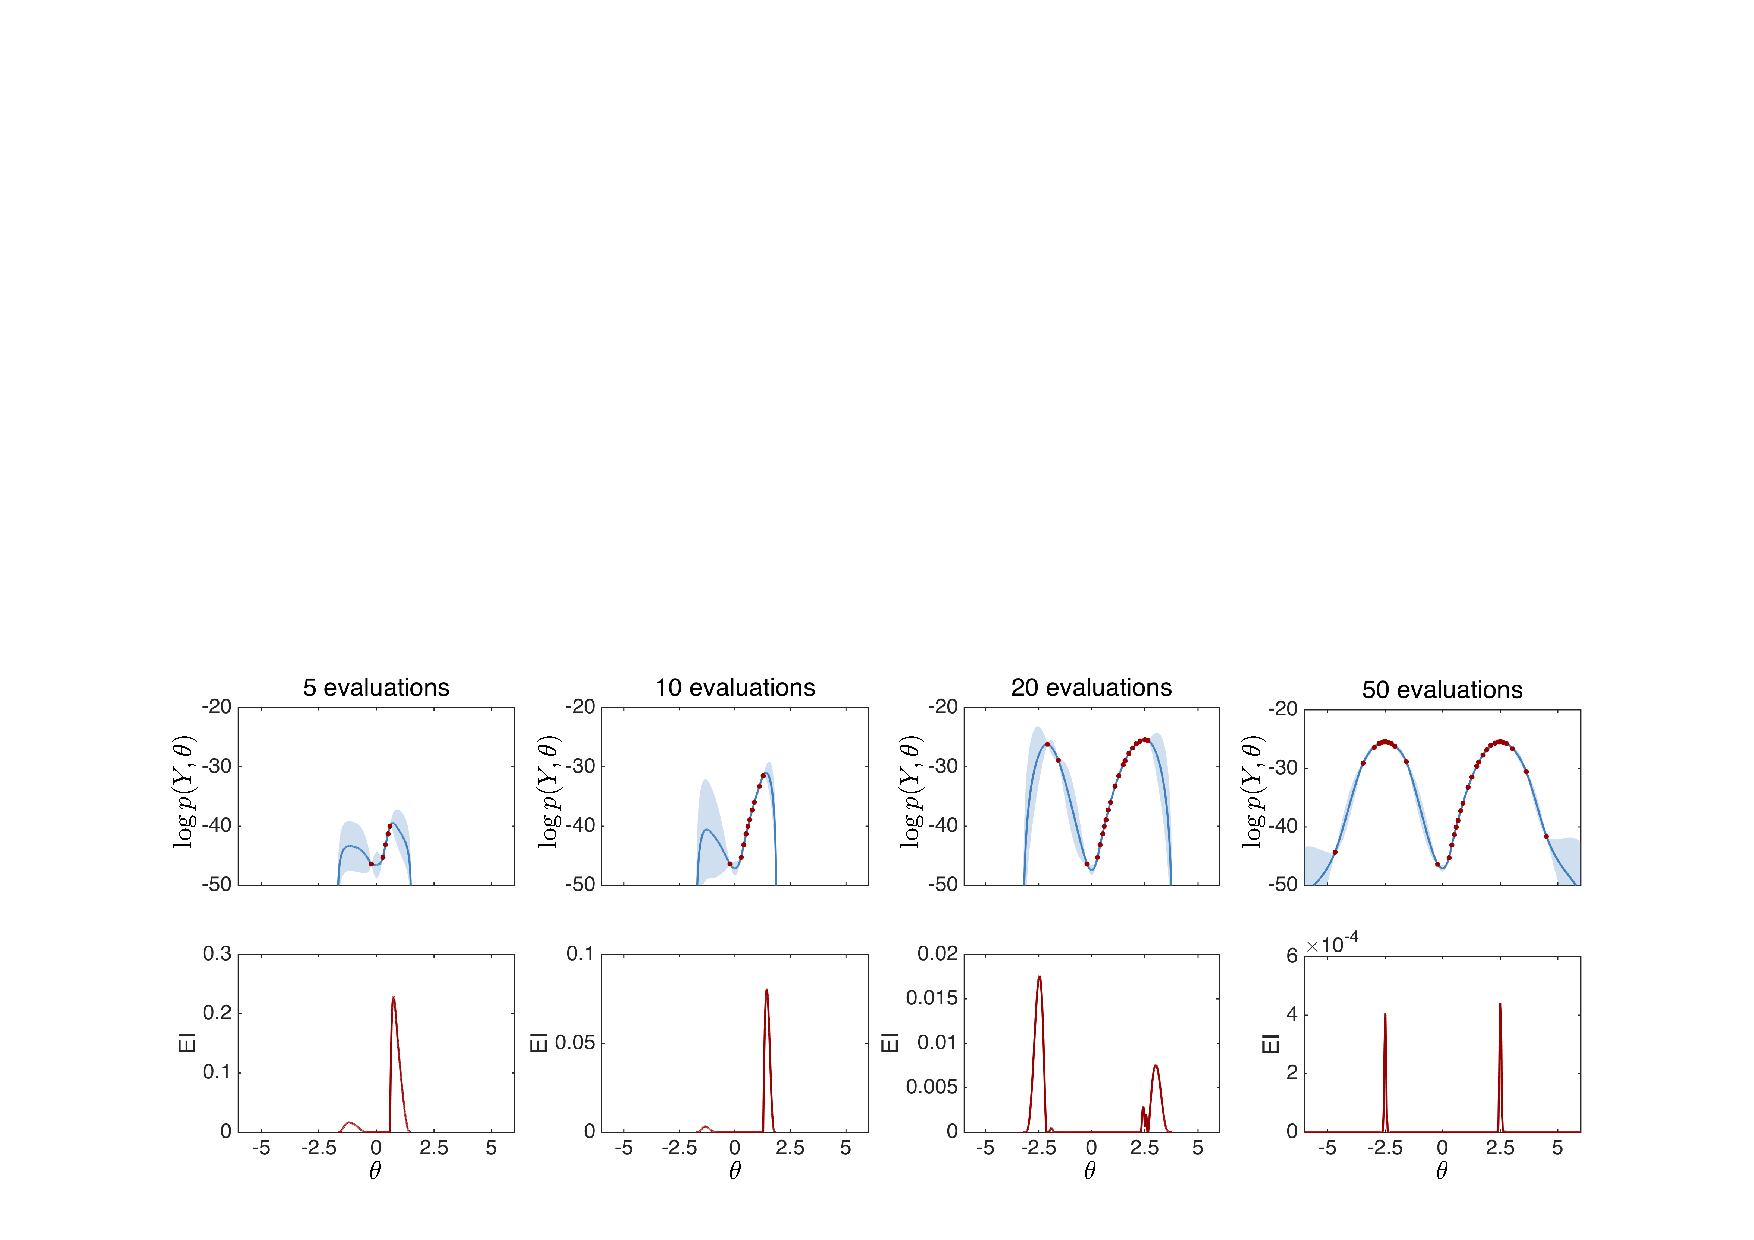
\includegraphics[width=0.99\textwidth]{unbounded_opt}
	\caption{Convergence on an unconstrained bimodal problem with $p \left(\theta\right)={\rm Normal}(0, 0.5)$ and $p \left(Y|\theta\right)={\rm Normal}(5-\left|\theta\right|,0.5)$ giving significant prior misspecification. The top plots show a regressed GP, with the solid line corresponding to the mean and the shading shows $\pm$ 2 standard deviations.  The bottom plots show the corresponding acquisition functions. \label{fig:domainAdpat}}
\end{figure*}

We first demonstrate the ability of BOPP to carry out unbounded optimization using a 1D problem with a significant prior-posterior mismatch as shown in Figure \ref{fig:domainAdpat}.  It shows BOPP adapting to the target and effectively establishing a maxima in the presence of multiple modes.   After 20 evaluations the acquisitions begin to explore the right mode, after 50 both modes have been fully uncovered.

\begin{figure*}[t]
	\centering
	
\includegraphics[width=1\textwidth]{combined_opt_plots}
	%	\includegraphics[width=1.35in]{figures/bayes-opt-comp/branin.pdf}
	%	\includegraphics[width=1.35in]{figures/bayes-opt-comp/hartmann.pdf}
	%	\includegraphics[width=1.35in]{figures/bayes-opt-comp/svm.pdf}
	%	\includegraphics[width=1.35in]{figures/bayes-opt-comp/lda.pdf}
	\caption{Comparison of BOPP  used as an optimizer to prominent BO packages on common benchmark problems.  
		%Branin and Hartmann 6D represent are continuous optimizations, whilst SVM on-grid and LDA on-grid are discrete.  
		The dashed lines shows the final mean error of SMAC (red), Spearmint (green) and TPE (black) as quoted by \cite{eggensperger2013towards}. % which also provides further details on the other packages and the benchmark problems.  
		The dark blue line shows the mean error for BOPP averaged over 100 runs, whilst the median and 25/75\% percentiles are shown in cyan. Results for Spearmint on Branin and SMAC on SVM on-grid are omitted because both BOPP and the respective algorithms averaged zero error to the provided number of significant figures in \cite{eggensperger2013towards}.
		%, meaning it not possible to check where BOPP performed better or worse then the alternative in these two cases.
		\label{fig:bayes-opt}}
\end{figure*}

\subsection{Classic Optimization Benchmarks}

Next we compare BOPP to the prominent BO packages SMAC \cite{hutter2011sequential}, Spearmint \cite{snoek2012practical} and TPE \cite{bergstra2011algorithms} on a number of classical benchmarks as shown in Figure \ref{fig:bayes-opt}.  These results demonstrate that BOPP provides substantial advantages over these systems when used simply as an optimizer on both continuous and discrete optimization problems.  In particular, it offers a large advantage over SMAC and TPE on the continuous problems (Branin and Hartmann), due to using a more powerful surrogate, and over Spearmint on the others due to not needing to make approximations to deal with discrete problems.

\subsection{Marginal Maximum a Posteriori Estimation Problems}

We now demonstrate application of BOPP on a number of MMAP problems.  Comparisons here are more difficult due to the dearth of existing alternatives for PPS.  In particular, simply running inference on the original query does not return estimates for $p\left(Y,\theta\right)$.  We consider the possible alternative of using our conditional code transformation to design a particle marginal Metropolis Hastings (PMMH, \cite{andrieu2010particle}) sampler which operates in a similar fashion to BOPP except that new $\theta$ are chosen using a MH step instead of actively sampling with BO.
%\footnote{To carry out MMAP one could further apply an annealing to the PMMH.  We omit this here as the behaviour of such as system would be indistinguishable from the presented results, due to the small number of iterations and very large variations of $p\left(\theta\right)$ for changes in $\theta$.}
For these MH steps we consider both LMH \citep{wingate2011lightweight} with proposals from the prior and the random-walk MH (RMH) variant introduced in Section~\ref{sec:proginf:str:lmh}.

\subsubsection{Hyperparameter Optimization for Gaussian Mixture Model}

% !TEX root =  bopp.tex


\begin{figure}[t]
	\begin{lstlisting}[basicstyle=\footnotesize\ttfamily]
(defopt mvn-mixture [data mu0 kappa psi] [nu alpha]
 (let [[n d] (shape data)
       alpha (sample (uniform-continuous 0.01 100))
       nu (sample (uniform-continuous (- d 1) 100))
       obs-proc0 (mvn-niw mu0 kappa nu psi)]
       (loop [data data
              obs-procs {}
              mix-proc (dirichlet-discrete 
                          (vec (repeat d alpha)))]
	    (let [y (first data)]
	     (if y
	      (let [z (sample (produce comp-proc))
	            obs-proc (get obs-procs z obs-proc0)
	            obs-dist (produce obs-proc)]
	        (observe obs-dist y)
	        (recur (rest data)
	               (assoc obs-procs z (absorb obs-proc y))
	        (absorb mix-proc z)))
	      mix-proc)))))
	\end{lstlisting}
	\caption{
		\label{fig:mvn-code}
		Anglican query for hyperparameter optimization of a Gaussian mixture model, defined in terms of two parameters \lsi{nu} and \lsi{alpha}. A \lsi{mvn-niw} process is used to represent the marginal likelihood of observations under a Gaussian-inverse-Wishart prior, whereas a \lsi{dirichlet-discrete} process models the prior probability of cluster assignments under a Dirichlet-discrete prior. The command \lsi{produce} returns the predictive distribution for the next sample from a process. \lsi{absorb} conditions on the value of the next sample.}
\end{figure}

\begin{figure*}[t]
	%	\includegraphics[width=1.7in]{"../figures/mvn-mixture/opt-nu-alpha-160229-01-10"}
	%	~
	%	\includegraphics[width=1.7in]{"../figures/mvn-mixture/opt-nu-alpha-160229-01-20"}
	%	~
	%	\includegraphics[width=1.7in]{"../figures/mvn-mixture/opt-nu-alpha-160229-01-50"}
	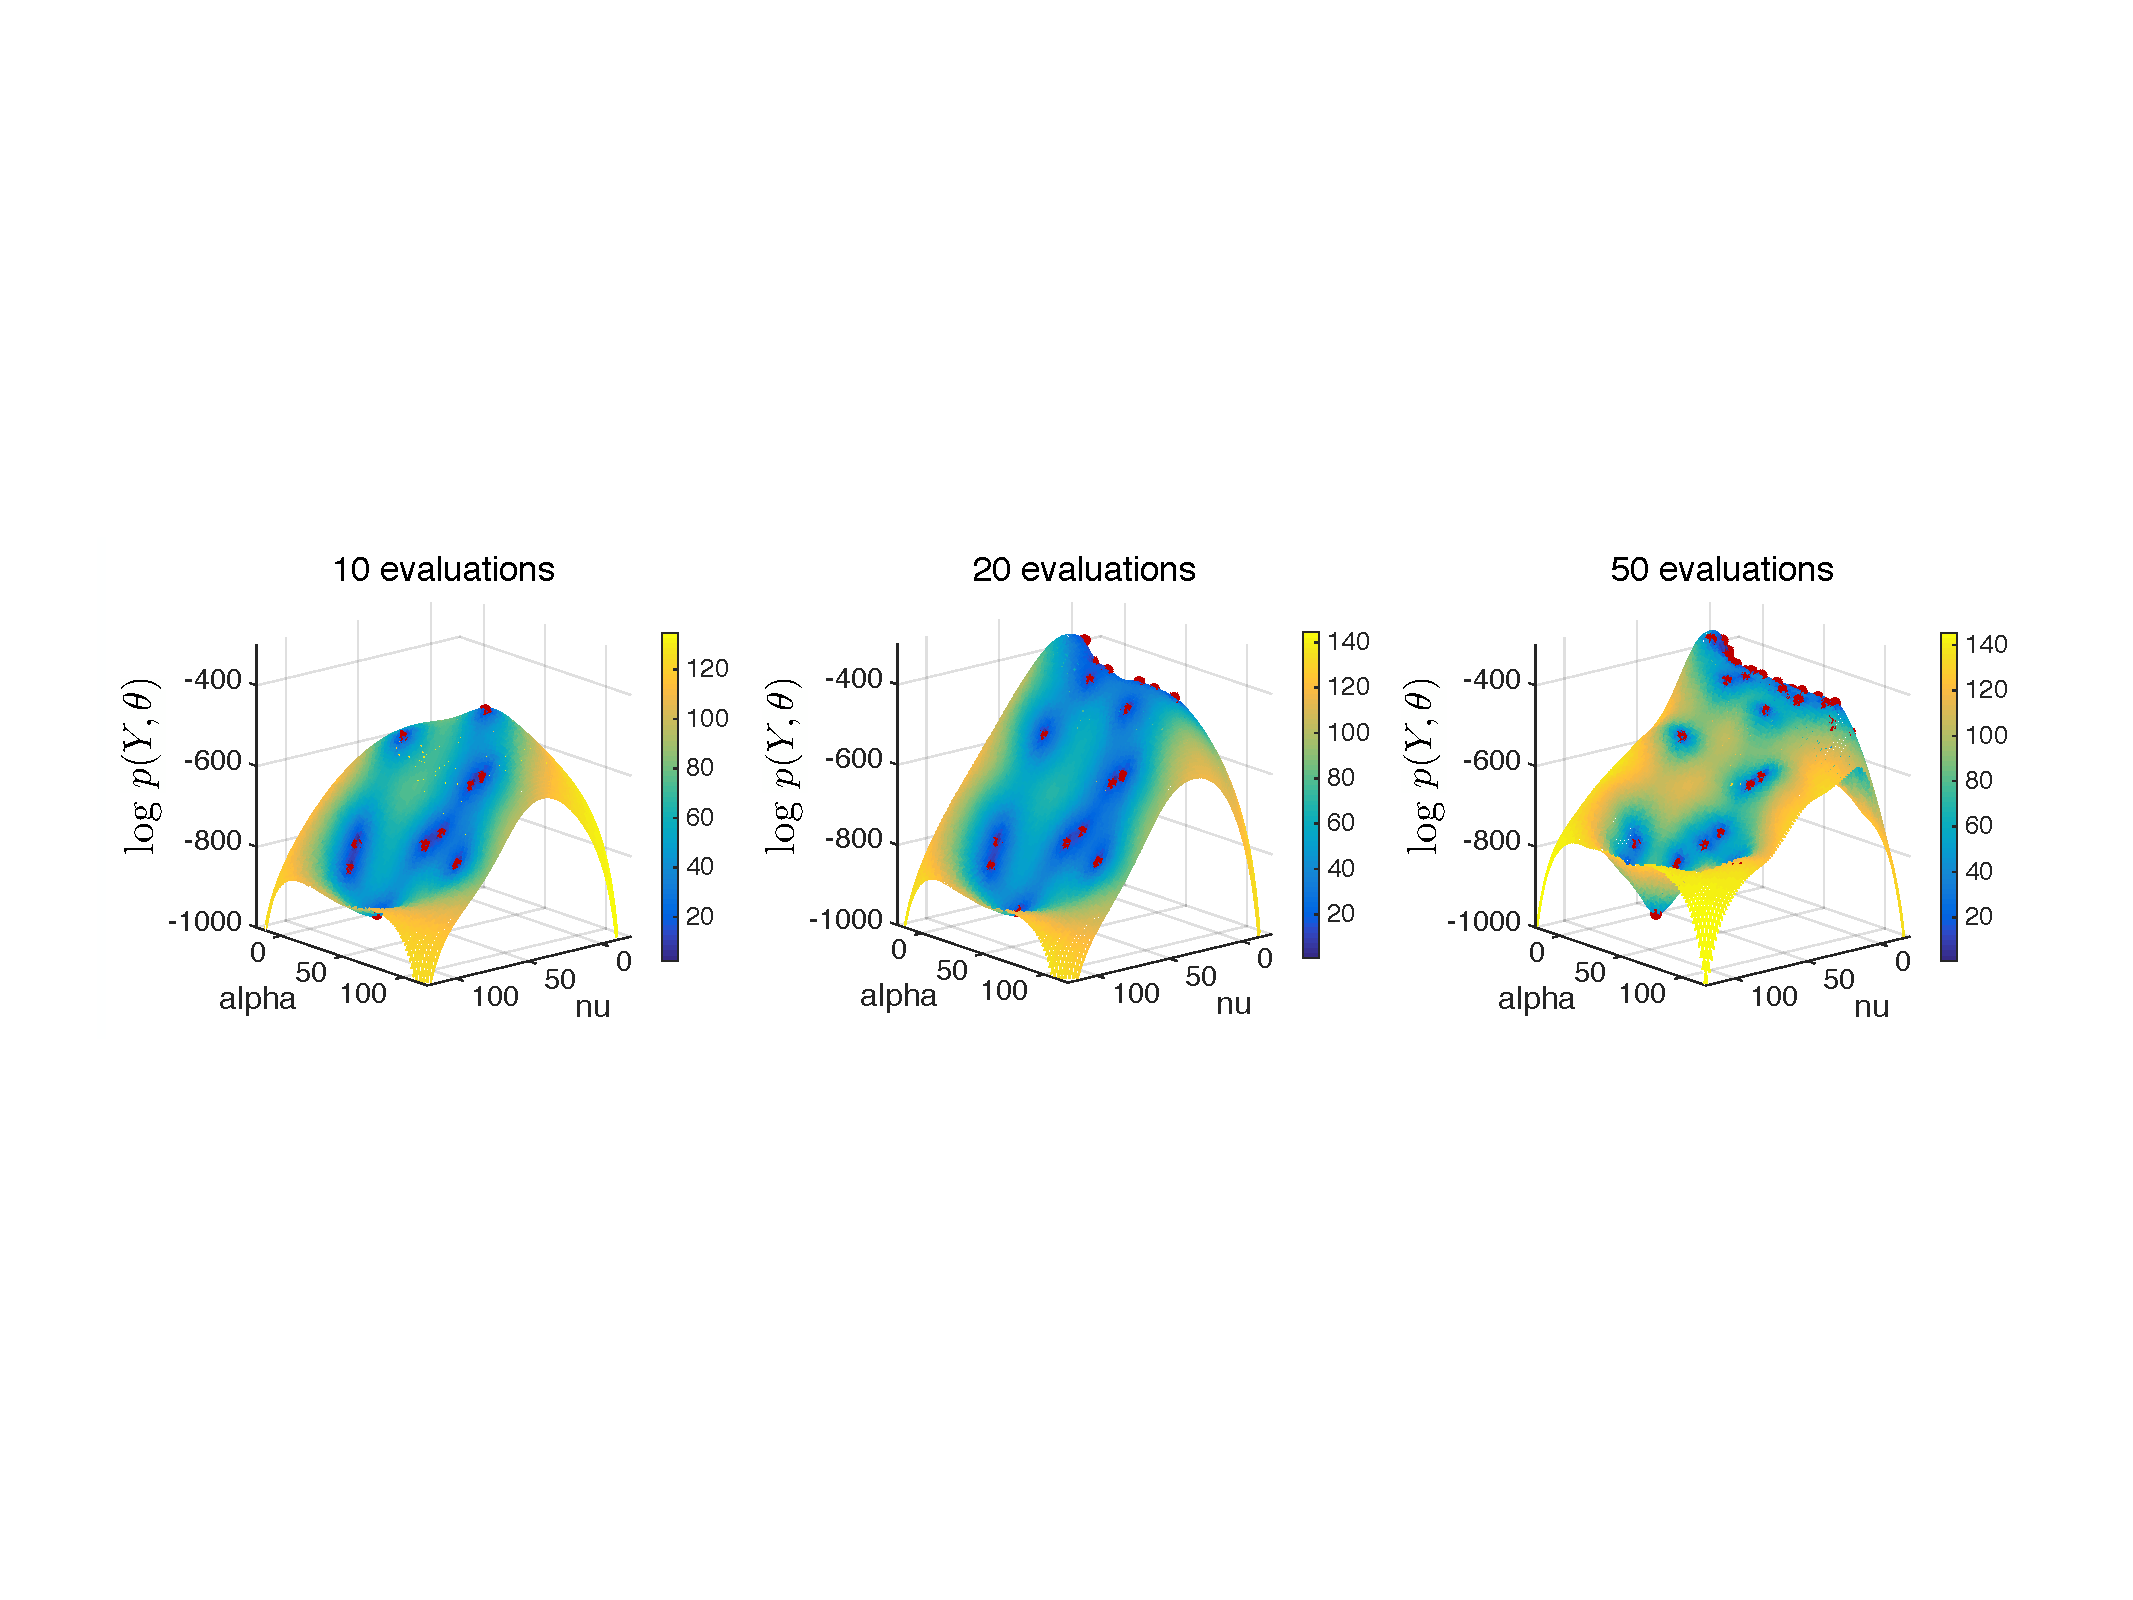
\includegraphics[width=\textwidth]{mvn-mixture/axis_corr_mvn_gps}
	\caption{
		\label{fig:mvn-gp-surface}
		Bayesian optimization of hyperparameters in a Gaussian mixture model evaluated on the Iris dataset. Panels show the GP posterior as a function of number of evaluations, with the surface corresponding to the posterior mean and the color bars the posterior standard deviation. Optimization is performed over the parameter $\alpha$ of a 10-dimensional symmetric Dirichlet distribution and the degrees of freedom $\nu$ of the inverse-Wishart prior. At each evaluation we obtain an estimate of the log marginal $\log p(Y,\theta)$ obtained by performing sequential Monte Carlo inference with 1000 particles.  The apparent maximum after initialization with 10 randomly sampled points lies at $\nu=31$, $\alpha=60$, and $\log p(Y,\theta) = -456.3$ (\emph{left}).  The surface after 10 optimization steps shows a new maximum at $\nu=9.2$, $\alpha=0.8$, and $\log p(Y,\theta) = -364.2$ (\emph{middle}). After 40 steps and 50 total evaluations this optimum is refined to $\nu=16$, $\alpha = 0.2$, and $\log p(Y,\theta) = -352.5$  (\emph{right}).}
\end{figure*}

We start with an illustrative case study of optimizing the hyperparameters in a multivariate Gaussian mixture model. We consider a Bayesian formulation with a symmetric Dirichlet prior on the mixture weights and a Gaussian-inverse-Wishart prior on the likelihood parameters:
\begin{align}
\v{\pi}
&\sim 
{\rm Dir(\alpha, \ldots, \alpha)}
\displaybreak[0]\\
(\v{\mu}_k, \v{\Sigma}_k)
&\sim 
{\rm NIW} (\v{\mu}_0, \kappa, \v{\Psi}, \nu)
&
{\rm for~}
&
k = 1, \ldots , K
\displaybreak[0]\\
z_n 
&\sim 
{\rm Disc(\v{\pi})}
\displaybreak[0]\\
\v{y}_n
&
\sim
{\rm Norm}(\v{\mu}_{z_n}, \v{\Sigma}_{z_n})
&
{\rm for~}
&
n = 1, \ldots , N
\end{align}
% Figure~\ref{fig:mvn-code} shows an optimization query for an Anglican program corresponding to this model. 
Anglican code for this model is shown in Figure 4. Anglican provides stateful objects, which are referred to as random processes, to represent the predictive distributions for the cluster assignments $z$ and the observations $\v{y}^k$ assigned to each cluster
\begin{align}
z_{n+1}
& \sim 
p( \cdot \,|\, z_{1:n}, \alpha),
\\
\v{y}_{m+1}^{k} 
& \sim 
p(\cdot \,|\, \v{y}^k_{1:m}, \v{\mu}_0, \kappa, \v{\Psi}, \nu).
\end{align}
In this collapsed representation marginalization over the model parameters $\v{\pi}$, $\v{\mu}_{k=1:K}$, and $\v{\Sigma}_{k=1:K}$ is performed analytically.
%The only variables that are sampled during program execution are the cluster assignments $z_{1:N}$, which we marginalize over using the general-purpose sequential Monte Carlo (SMC) implementation provided by the inference back end. 
%Like any importance sampling method, SMC provides an unbiased estimate $\hat Z$ of the marginal likelihood $Z = p(\v{y}_{1:N} | \alpha, \v{\mu}, \kappa, \v{\Psi}, \nu)$. 
%Intuitively, the parameter $\nu$, which is known as the degrees of freedom, represents a scale factor for the covariance matrix, which determines the spatial extent of the clusters (larger $\nu$ values imply a smaller covariance and cluster size). 
%The parameter $\alpha$, sometimes known as a concentration parameter, controls the distribution on mixture weights (where $\alpha \gg 1.0$ implies an even distribution and $\alpha \ll 1.0$ implies an uneven distribution).  
Using the Iris dataset, a standard benchmark for mixture models that contains 150 labeled examples with 4 real-valued features, we optimize the marginal with respect to the subset of the parameters $\nu$ and $\alpha$ under uniform priors over a fixed interval.  For this model, BOPP aims to maximize
\begin{align}
\begin{split}
& p(\nu, \alpha | \v{y}_{n=1:N}, \v{\mu}_0, \kappa, \v{\Psi}) \\
&= \iiiint p(\nu, \alpha, z_{n=1:N}, \v{\pi}, \v{\mu}_{k=1:K}, \v{\Sigma}_{k=1:K} | \v{y}_{n=1:N}, \mu_0, \kappa, \v{\Psi}) \mathrm{d}z_{n=1:N}\mathrm{d}\v{\pi}\mathrm{d}\v{\mu}_{k=1:K}\mathrm{d}\v{\Sigma}_{k=1:K}.
\end{split}
\end{align}

Figure~\ref{fig:mvn-gp-surface} shows GP regressions on the evidence after different numbers of the SMC evaluations have been performed on the model.  This demonstrates how the GP surrogate used by BO builds up a model of the target, used to both estimate the expected value of $\log p(Y,\theta)$ for a particular $\theta$ and actively sample the $\theta$ at which to undertake inference.

% n=10
% x1_max: 30.90
% x2_max: 61.55
% y_max: -456.32
% mu_max: -456.33
% sig_max: 0.51

% n=20
% x1_max: 9.20
% x2_max: 0.79
% y_max: -364.21
% mu_max: -364.23
% sig_max: 0.47

% n=50
% x1_max: 16.34
% x2_max: 0.21
% y_max: -352.51
% mu_max: -352.51
% sig_max: 0.53

% n=100
% x1_max: 16.34
% x2_max: 0.21
% y_max: -352.51
% mu_max: -352.50
% sig_max: 0.41

% \begin{figure}
% \begin{lstlisting}[basicstyle=\footnotesize\ttfamily]
% (defopt mvn-mixture 
%  [data mu kappa psi] [:nu :alpha]
%  (let [[n d] (shape data)
%        alpha (sample :alpha
%               (uniform-continuous 0.01 100))
%        nu (sample :nu 
%            (uniform-continuous (- d 1) 100))
%        obs-proc0 (mvn-niw mu kappa nu psi)]
%   (loop [data data
%          obs-procs {}
%          mix-proc (dirichlet-discrete 
%                    (vec (repeat d alpha)))]
%    (let [y (first data)]
%     (if y
%      (let [z (sample (produce comp-proc))
%            obs-proc (get obs-procs 
%                      z obs-proc0)
%            obs-dist (produce obs-proc)]
%       (observe obs-dist y)
%       (recur (rest data)
%              (assoc obs-procs
%                z (absorb obs-proc y))
%              (absorb mix-proc z)))
%      (predict mix-proc))))))
% \end{lstlisting}
% \caption{
% \label{fig:mvn-code}
% Anglican query for hyperparameter optimization of a Gaussian mixture model, defined in terms of two parameters \lsi{:nu} and \lsi{:alpha}. A \lsi{mvn-niw} process is used to represent the marginal likelihood of observations under a Gaussian-inverse-Wishart prior, whereas a \lsi{dirichlet-discrete} process models the prior probability of cluster assignments under a Dirichlet-discrete prior. The command \lsi{produce} returns the predictive distribution for the next sample from a process. \lsi{absorb} conditions on the value of the next sample.}
% \end{figure}





% 


\subsubsection{Extended Kalman Filter for the Pickover Chaotic Attractor}
\label{sec:AppKalman}

% !TEX root =  ../main.tex


\begin{figure*}[t]
	\centering
	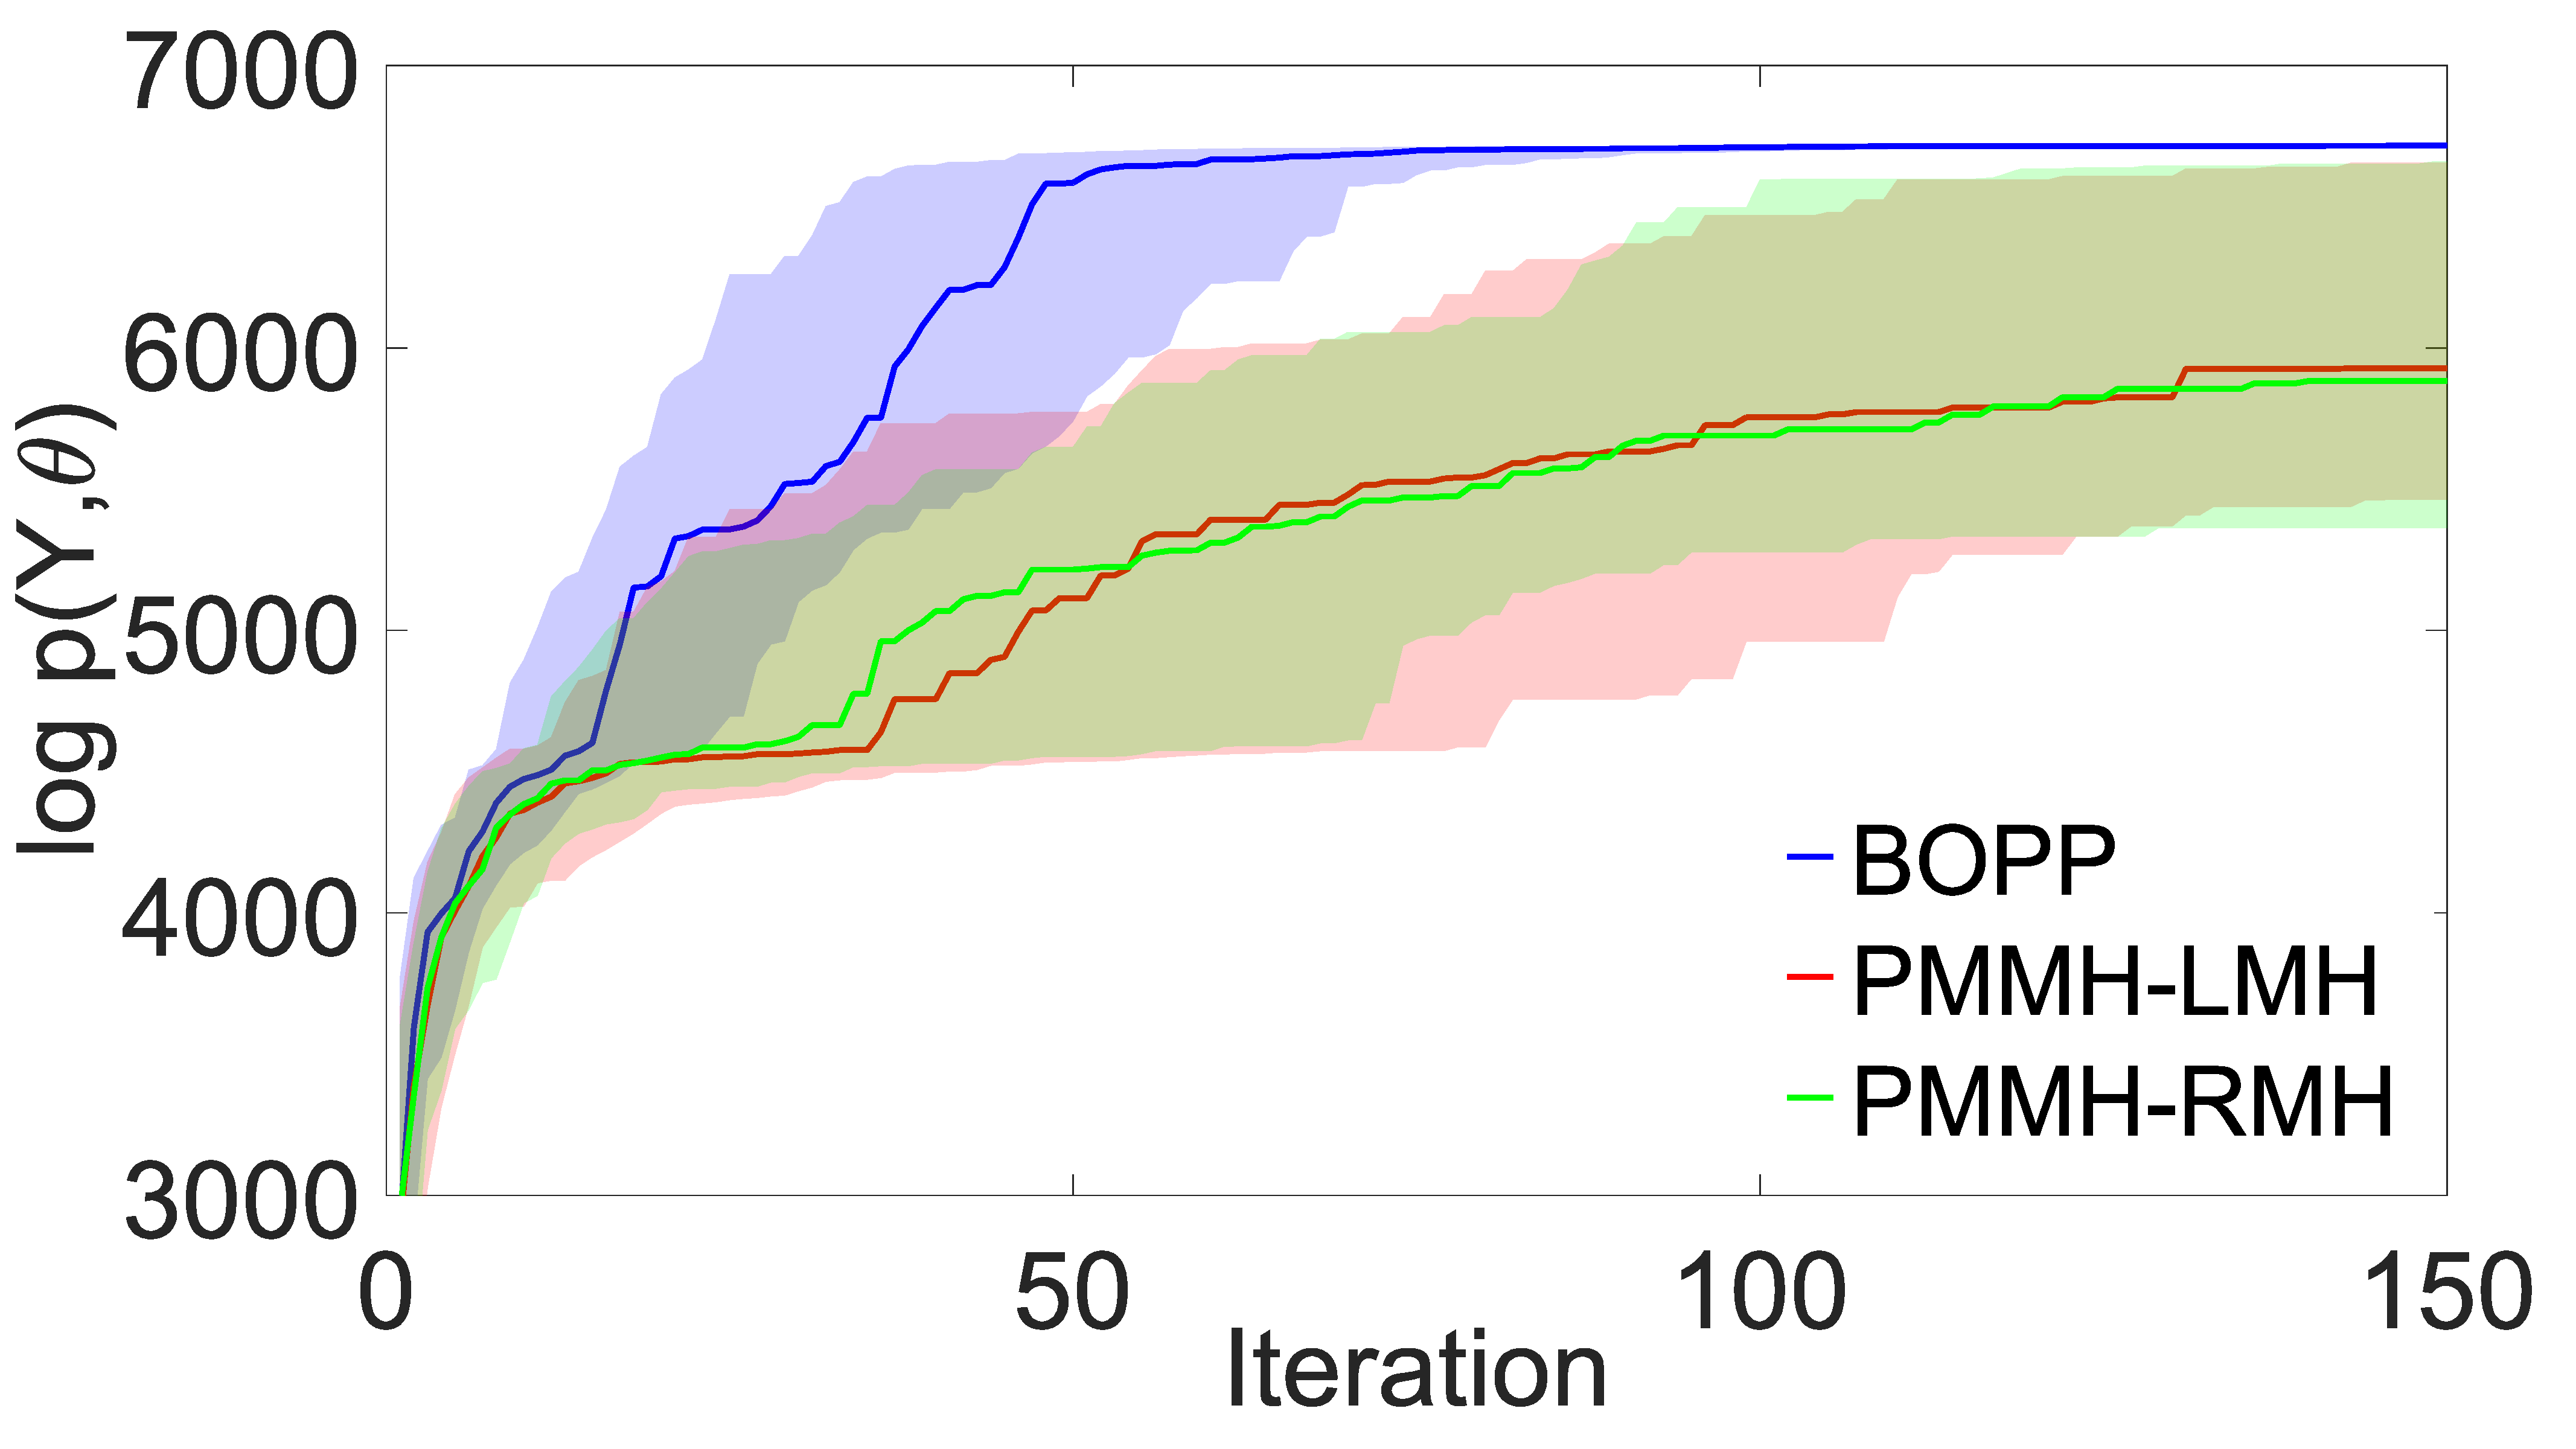
\includegraphics[width=2.72in]{chaos/chaos_ml.pdf}
	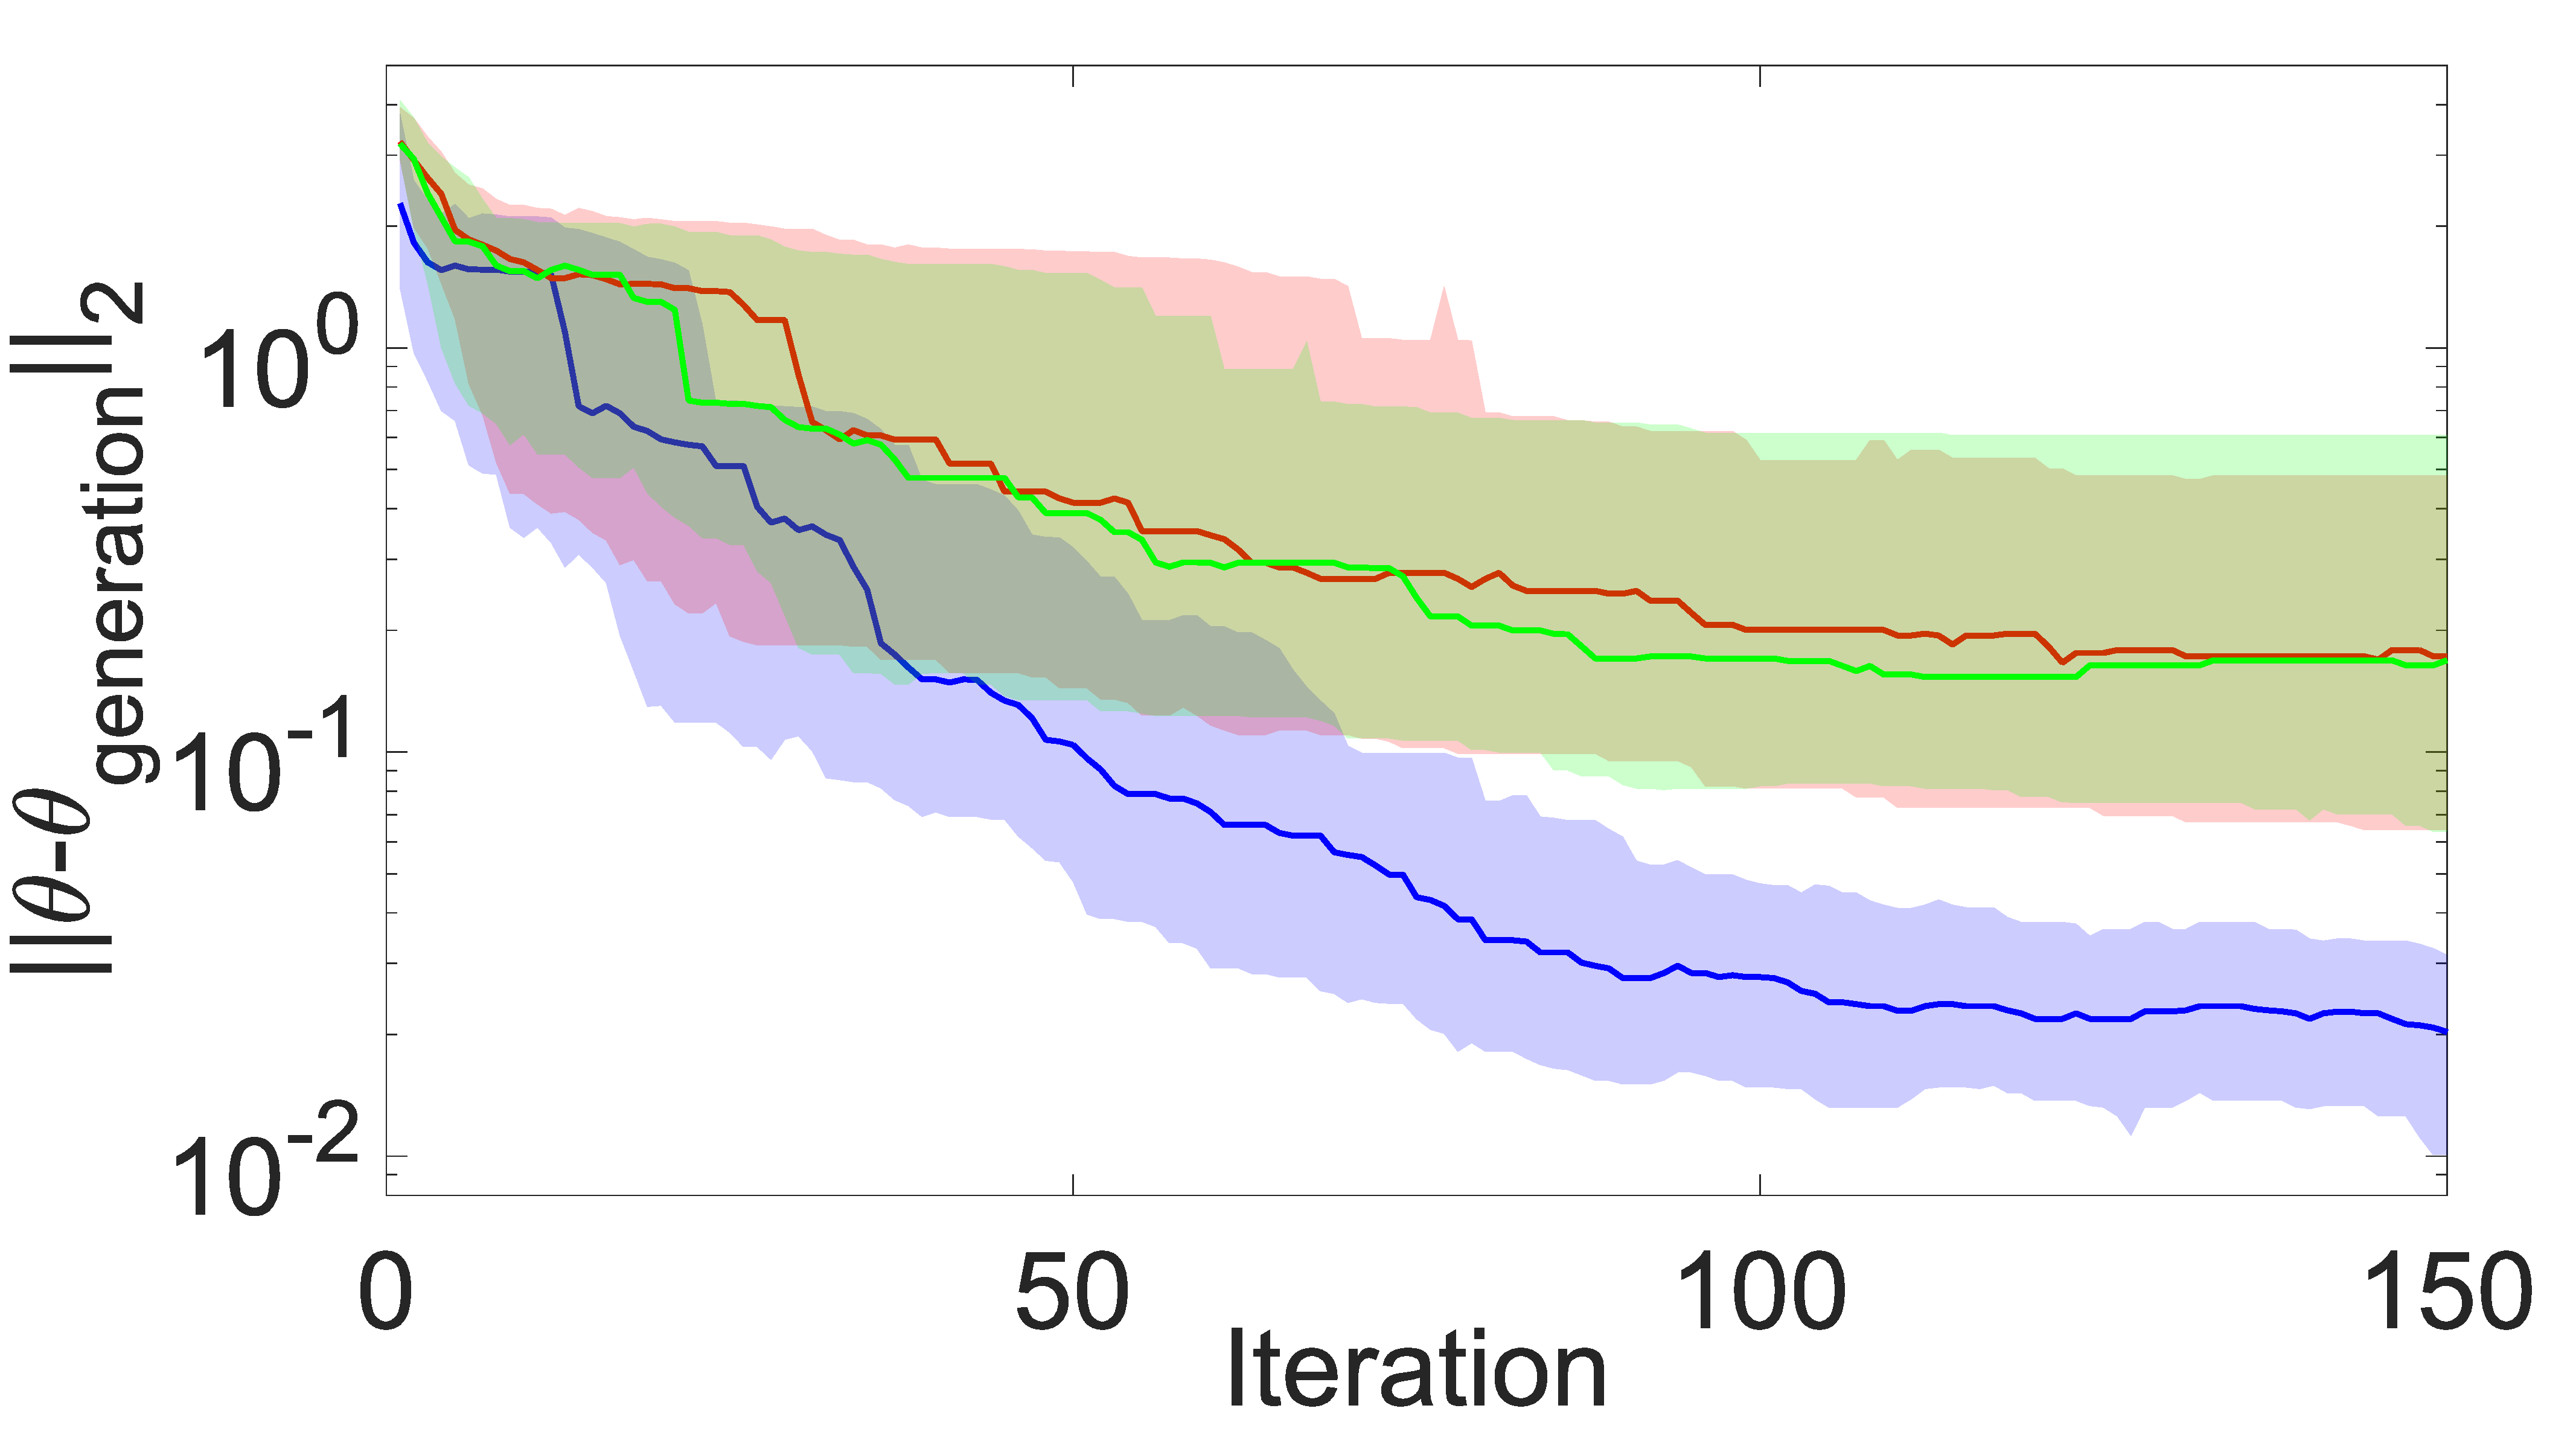
\includegraphics[width=2.72in]{chaos/chaos_distance.pdf}
	\caption{Convergence for transition dynamics parameters of the pickover attractor in terms of the cumulative best $\log p\left(Y,\theta\right)$ (\emph{left}) and distance to the ``true" $\theta$ used in generating the data (\emph{right}). Solid line shows median over 100 runs, whilst the shaded region the 25/75\% quantiles.  \label{fig:chaos}
		\vspace{6pt}}
\end{figure*}

\begin{figure}[t]
	\centering
	\begin{subfigure}[t]{0.24\textwidth}
		\centering
		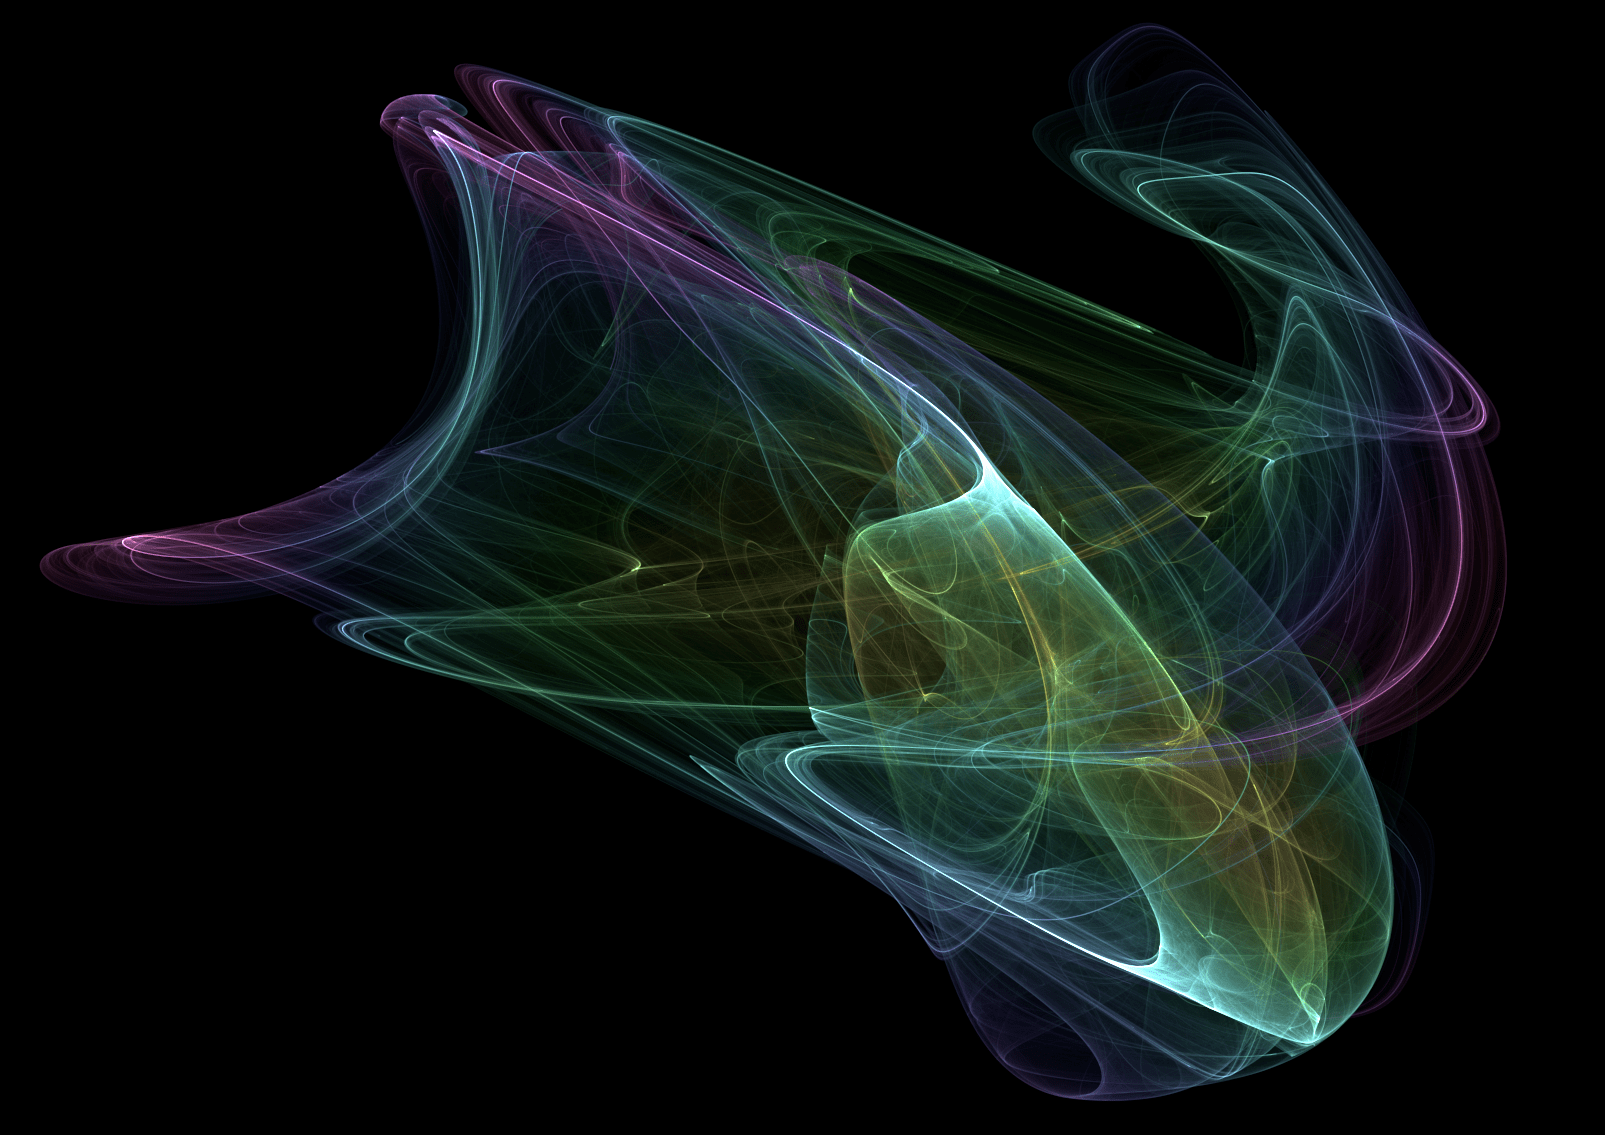
\includegraphics[height=3.2cm,width=3.7cm]{chaos/compressed/first_iter_alt.png}
		\caption{1 iteration}
	\end{subfigure}
	\begin{subfigure}[t]{0.24\textwidth}
		\centering
		\tiny
		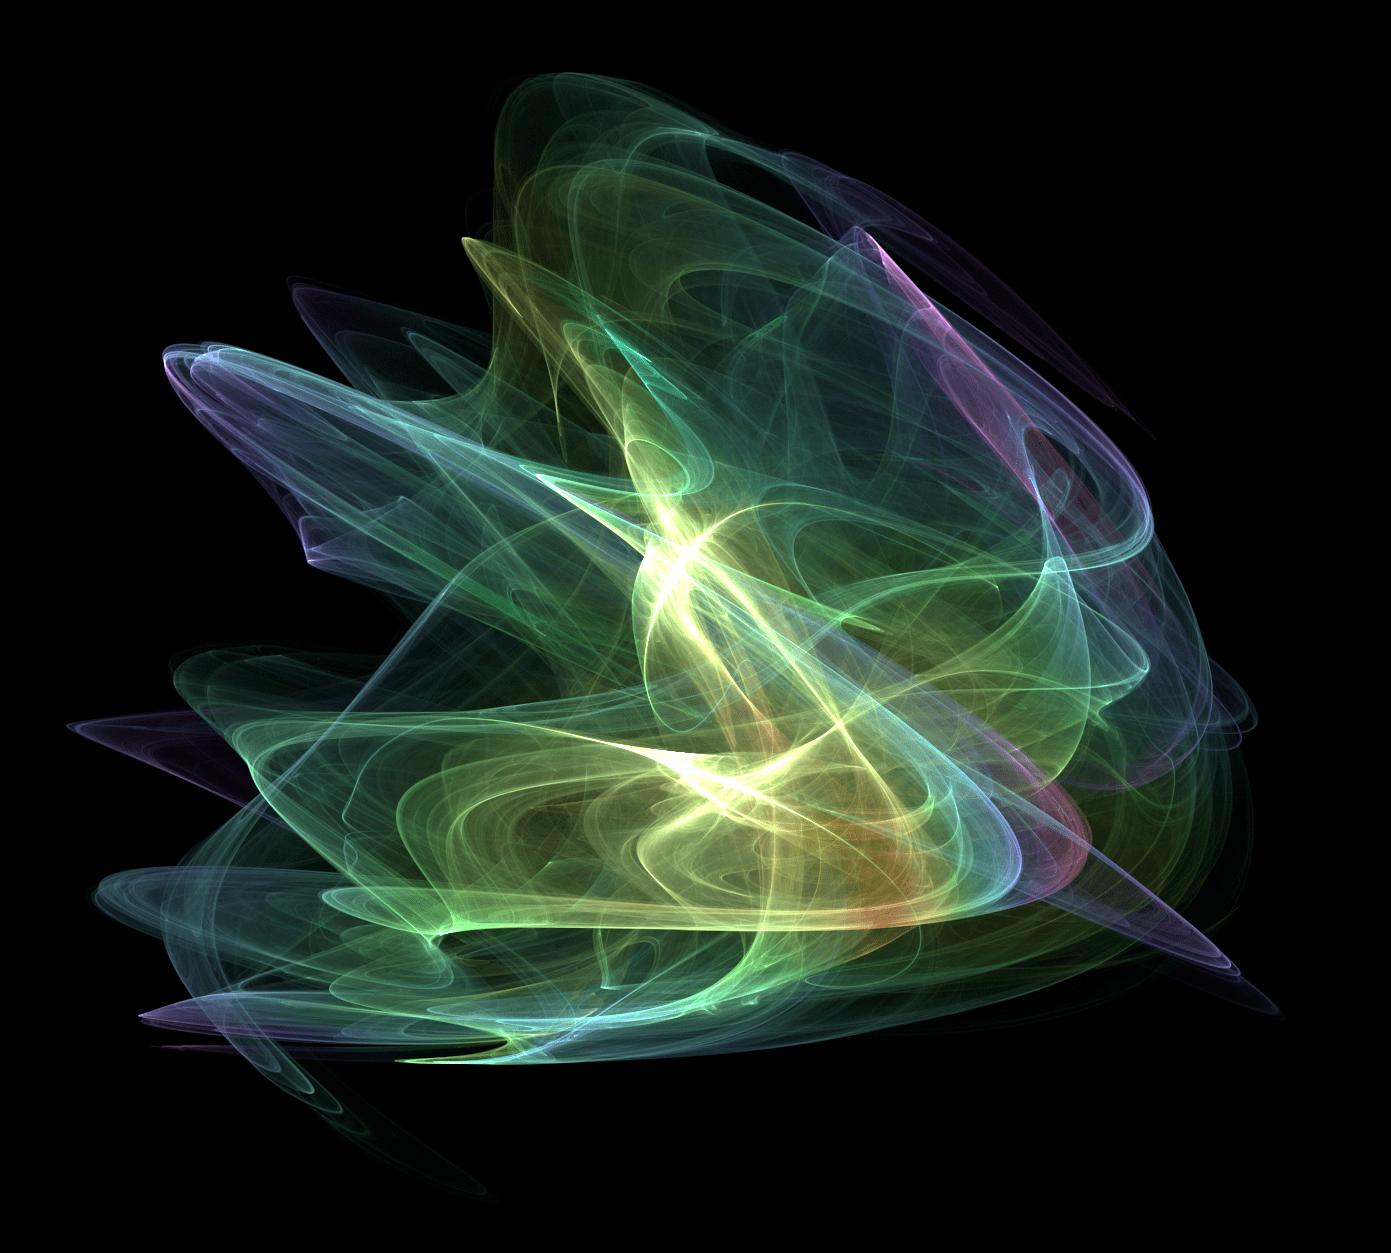
\includegraphics[height=3.2cm,width=3.7cm]{chaos/compressed/20_iter_alt.png}
		\caption{20 iterations}
	\end{subfigure}
	\begin{subfigure}[t]{0.24\textwidth}
		\centering
		\tiny
		
\includegraphics[height=3.2cm,width=3.7cm]{chaos/compressed/100_iter_altj.png}
		\caption{100 iterations}
	\end{subfigure}
	\begin{subfigure}[t]{0.24\textwidth}
		\centering
		\tiny
		
\includegraphics[height=3.2cm,width=3.7cm]{chaos/compressed/target_light.png}
		\caption{Ground truth}
	\end{subfigure}
	\caption{A series of trajectories for different parameters, demonstrating convergence to the true attractor.  The colormap is based on the speed and curvature of the trajectory, with rendering done using the program Chaoscope (available at {\href{http://www.chaoscope.org/}{http://www.chaoscope.org/}}). \label{fig:chaoscope}}
\end{figure}

Our first MMAP example considers the case of learning the dynamics parameters of a chaotic attractor.  
This constitutes a class Markovian state space model problem, specifically a Kalman smoother,
where we observe a noisy signal 
$y_t \in \real^{K}, \; t = 1,2,\dots,T$ in some $K$ dimensional observation space were each 
observation has a lower dimensional latent parameter $x_t \in \real^{D},  \; t = 1,2,\dots,T$.
In addition to an initial distribution $x_1 \sim \mathcal{N} \left(\mu_1, \sigma_1 I\right)$, our model is specified by 
\begin{subequations}
	\label{eq:Kalman}
\begin{align}
x_t = & A \left(x_{t-1}, \theta\right)+\delta_{t-1}, \; & \delta_{t-1} \sim \mathcal{N} \left(0, \sigma_q I\right) \\
y_t = & C x_{t}+\varepsilon_{t}, \; & \varepsilon_{t} \sim \mathcal{N} \left(0, \sigma_y I\right)
\end{align}
\end{subequations}
where $I$ is the identity matrix, $C$ is a known $K \times D$ matrix, and $\mu_1,\sigma_1, \sigma_q$ 
and $\sigma_y$ are all known scalars.  Our aim is to learn the dynamics parameters $\theta$ given
$y_{1:T}$, marginalizing over the latent variables $x_{1:T}$.  We use
a uniform prior on the parameters $\theta$, which means that the MMAP values for $\theta$
coincide with their (constrained) MML values.  A synthetic dataset was generated with $T=500$ and
$K=20$ (see \cite{rainforth2017boppArxiv}).
Inference on \qmarg was carried out using SMC with 500 particles.  
Convergence results are given in Figure~\ref{fig:chaos} showing that BOPP comfortably 
outperforms the PMMH variants, while Figure~\ref{fig:chaoscope} shows the simulated 
attractors generated from the dynamics parameters output by various iterations of a 
particular run of BOPP.


\subsubsection{Hidden Markov Model with Unknown Number of States}

% !TEX root =  ../main.tex

\begin{figure*}[t]
	\centering
	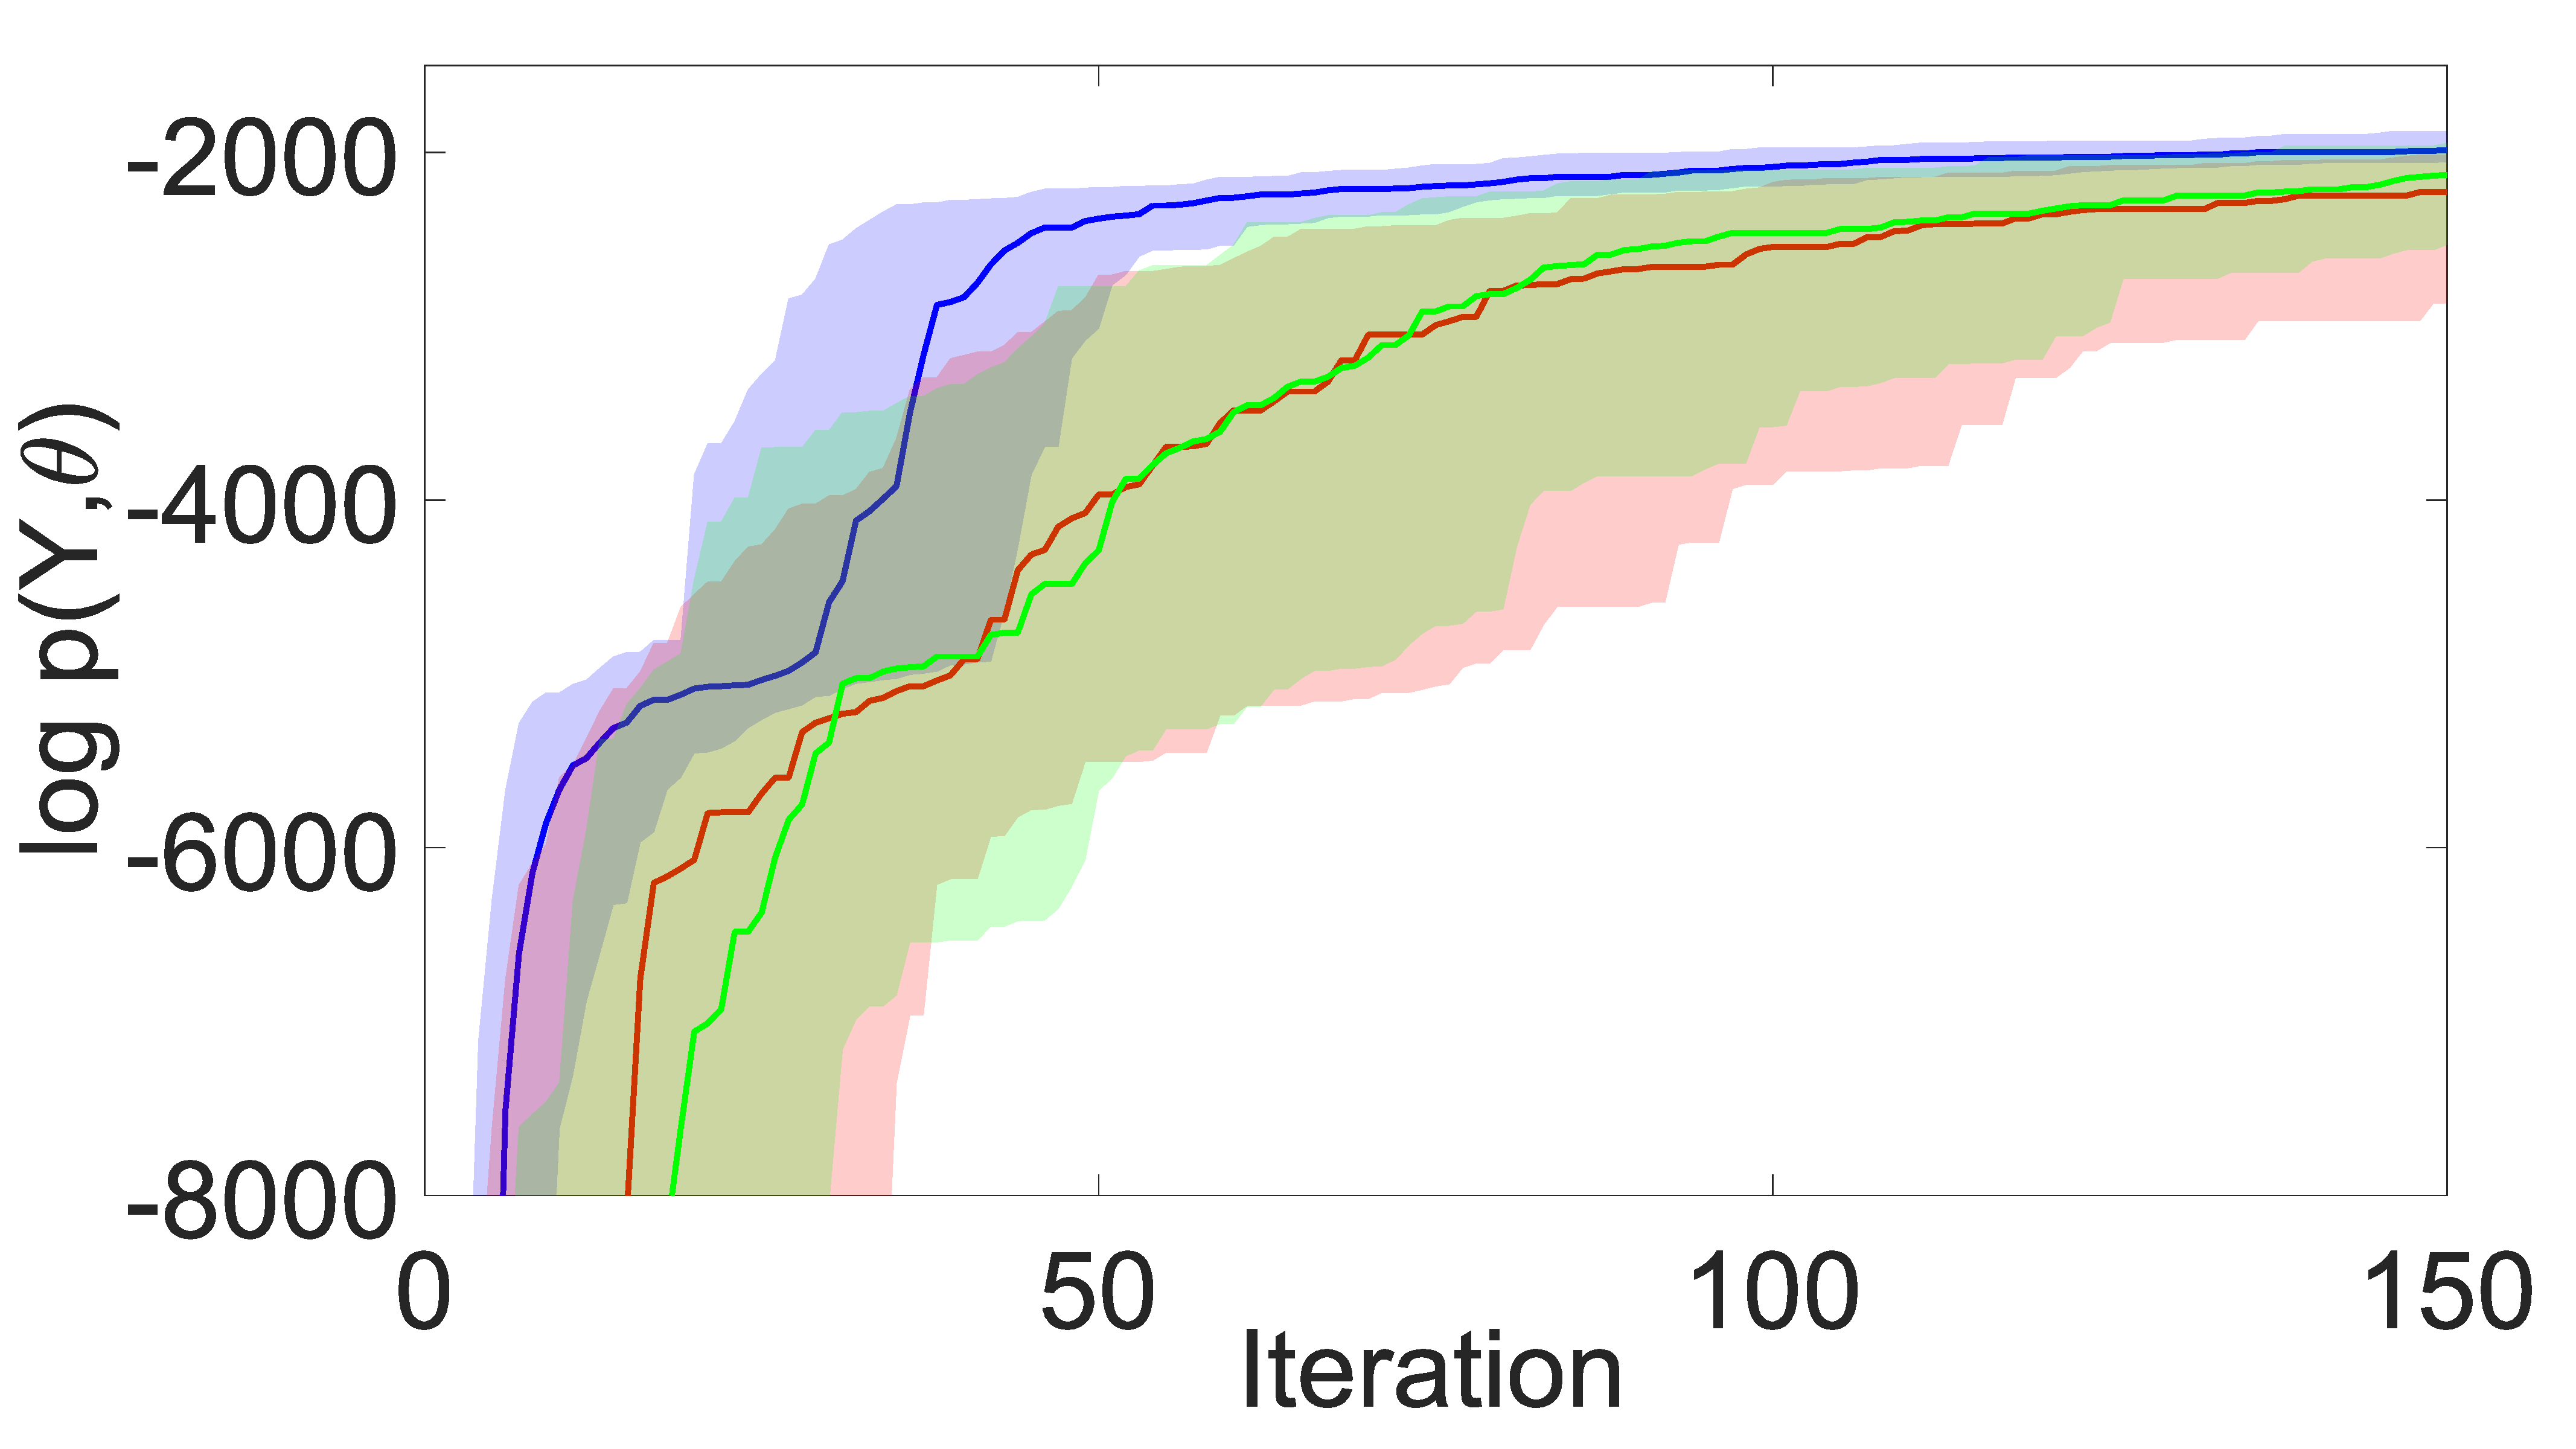
\includegraphics[width=2.72in]{hmm/hmm_ML}
	~~~~~~
	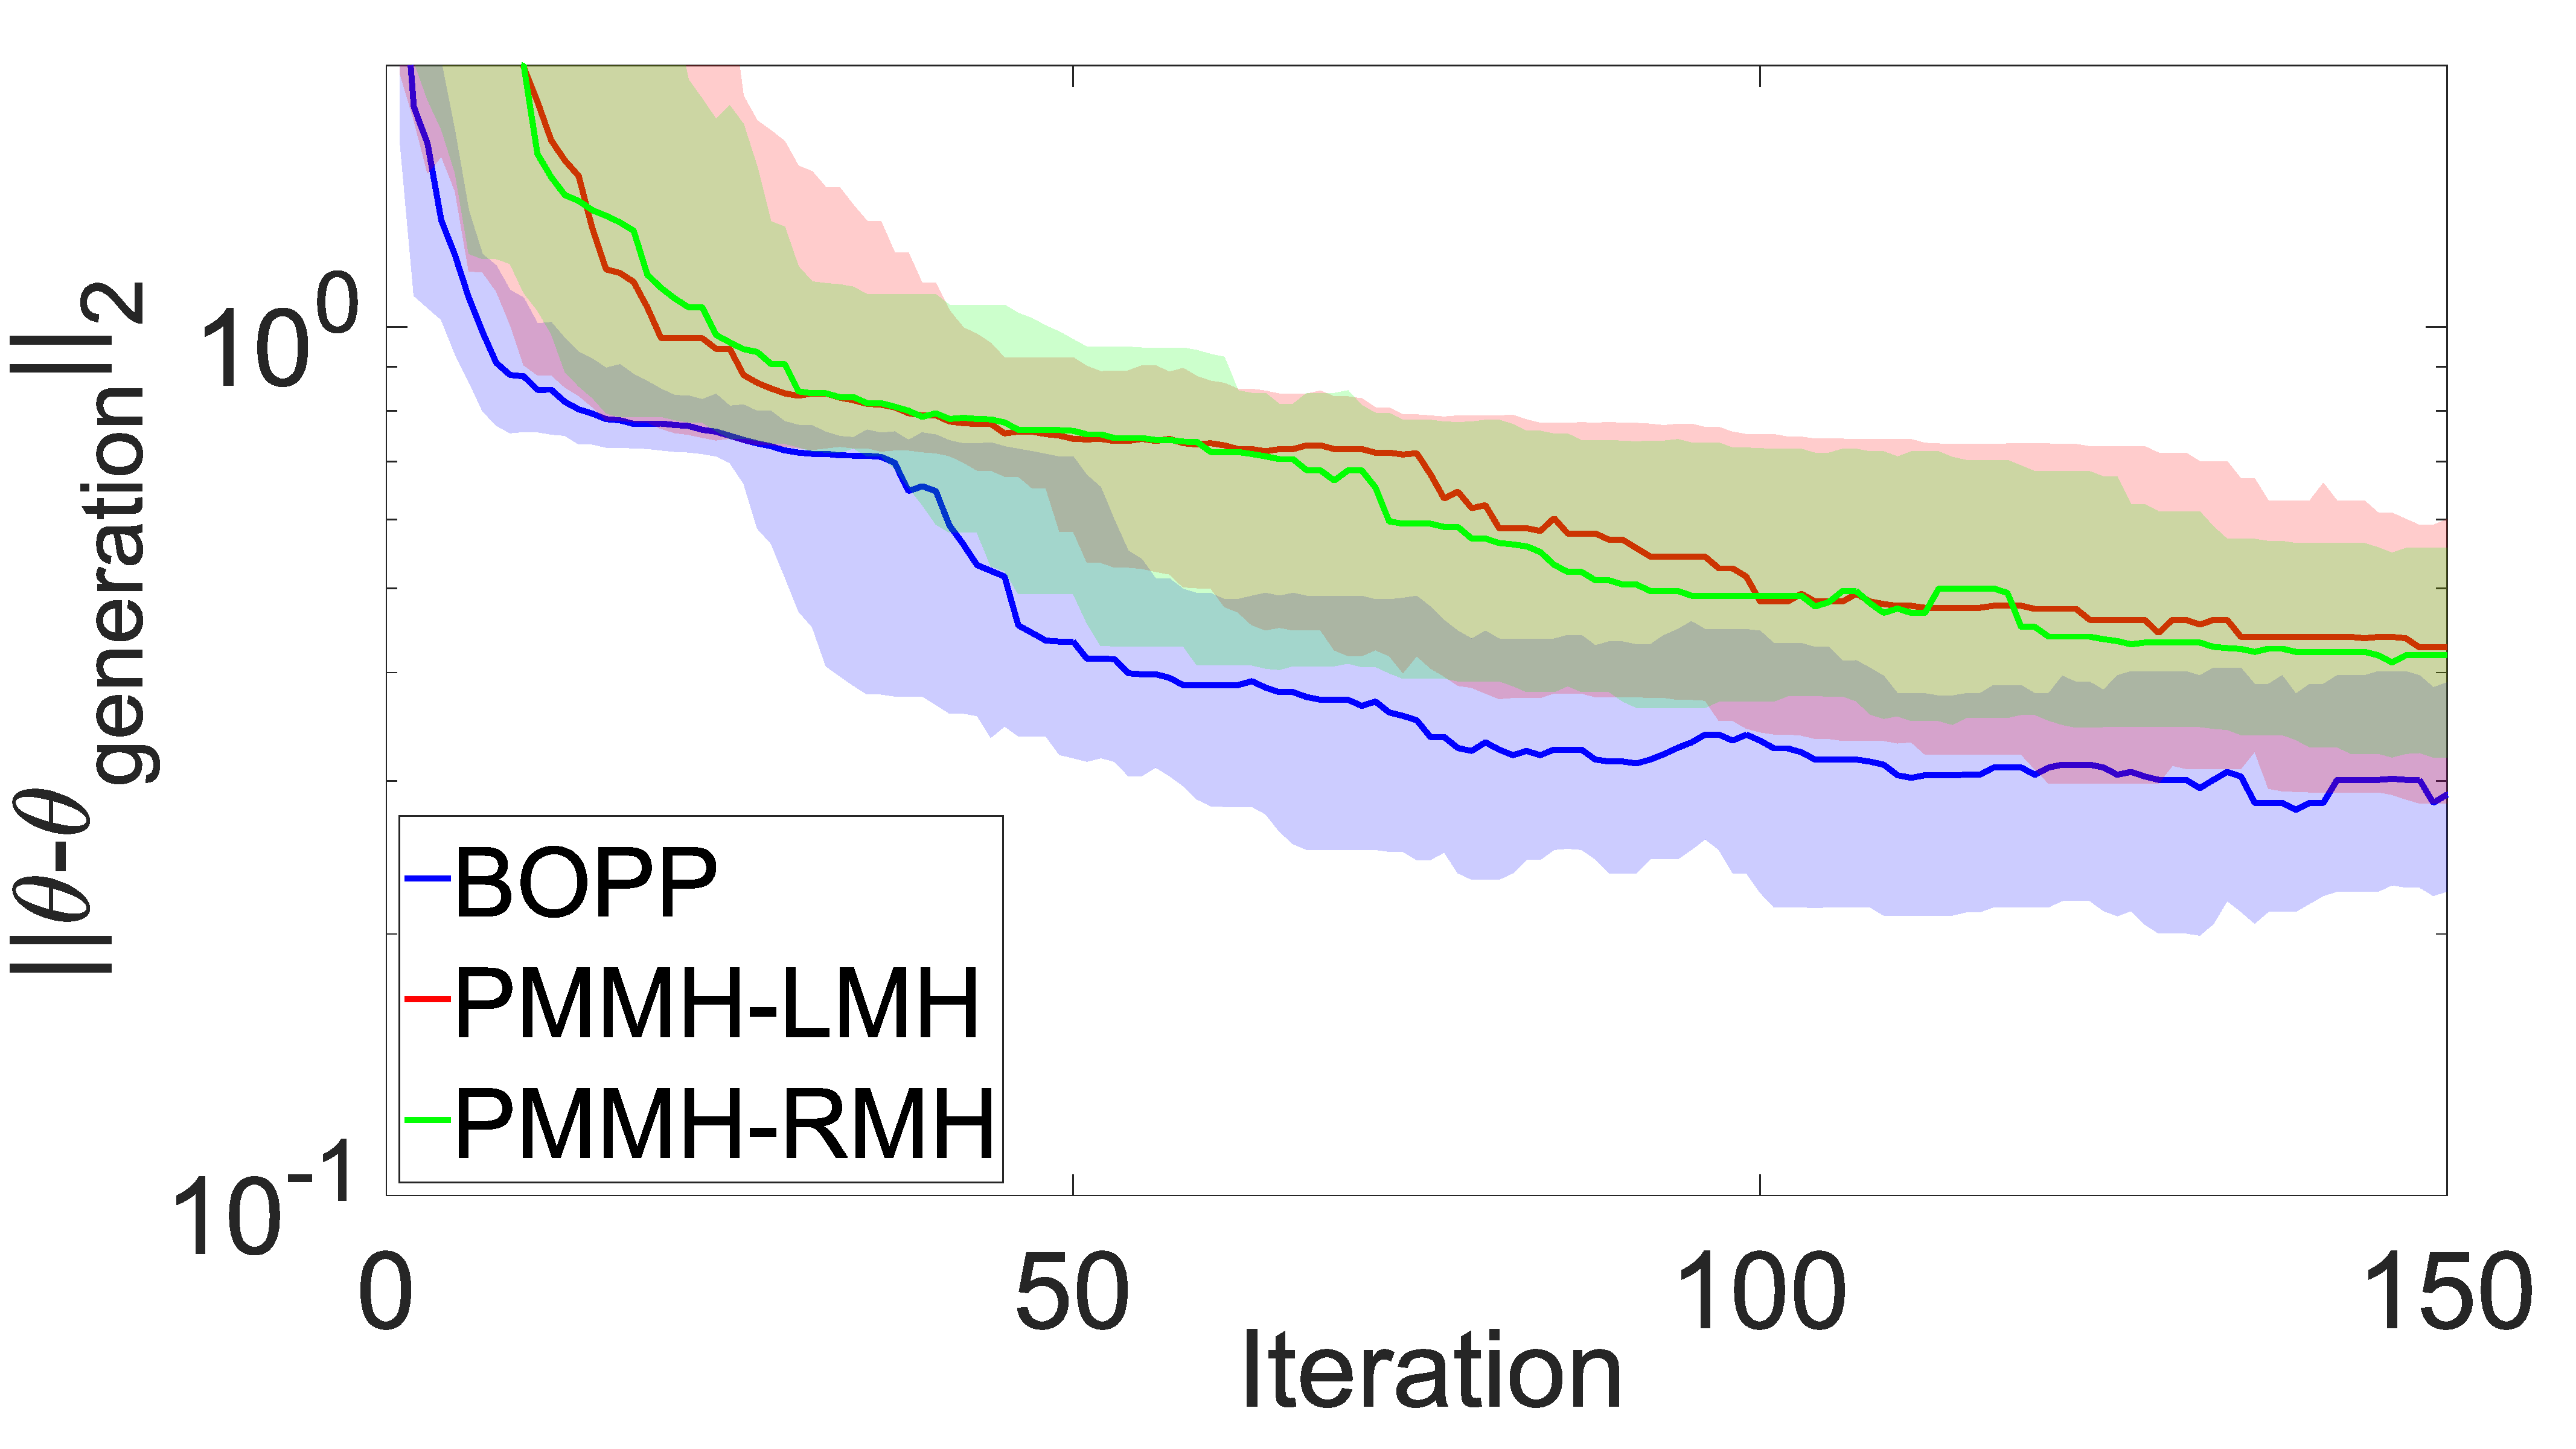
\includegraphics[width=2.72in]{hmm/hmm_distance}
	\caption{Convergence for HMM in terms of the cumulative best $\log p\left(Y,\theta\right)$ (\emph{left}) and distance to the ``true" $\theta$ used in generating the data (\emph{right}). Solid line shows median over 100 runs, whilst the shaded region the 25/75\% quantiles.  Note that for the distance to true $\theta$ was calculated by selecting the three states (out of the 5 generated) that were closest to the true parameters.  \label{fig:hmm}}
\end{figure*}

We finish by considering a hidden Markov model (HMM) with an unknown number of discrete possible states.  
This example demonstrates how BOPP can still be applied to models which conceptually have an 
unknown number of target variables, by generating all possible variables that might be needed, 
but then leaving some variables unused for some execution traces.  This avoids problems 
of varying reference measures so that the MMAP problem is well defined  and provides a 
function with a fixed number of inputs as required by the BO scheme.  From the BO 
perspective, the target function is simply constant for variations in an unused variable.

Our model places a uniform prior on the number of states $K \sim \textsc{Discrete}\{1,2,3,4,5\}$.
Each emission distribution corresponds to a Gaussian with unknown mean (which we wish to
optimize) and known variance.  
We marginalize over are the transition distribution parameters and the HMM latent states.  
Rather than constructing a model were the emission distribution
parameters only exist conditioned on the value of $K$, we generate variables for all $5$ emission
distributions that might be required, with only the first $K$ actually then used.  
A synthetic dataset was generated using $K=3$ and $T=1000$ observations.  Results of running BOPP are given
in Figure~\ref{fig:hmm}, again showing that BOPP outperforms these PMMH alternatives.  See~\cite{rainforth2017boppArxiv}
for further details.


%
%\subsection{Full Details for House Heating Experiment}
%\label{sec:app:heating}
%
%% !TEX root =  bopp.tex

In this case study, illustrated in Figure~\ref{fig:houses}, we optimize the parameters of a stochastic engineering simulation. We use the Energy2D system from \cite{xie2012energy2d} to perform finite-difference numerical simulation of the heat equation and Navier-Stokes equations in a user-defined geometry. 

In our setup, we designed a 2-dimensional representation of a house with 4 interconnected rooms using the GUI provided by Energy2D. The left side of the house receives morning sun, modelled at a constant incident angle of $30^\circ$. We assume a randomly distributed solar intensity and simulate the heating of a cold house in the morning by 4 radiators, one in each of the rooms. The radiators are given a fixed budget of total power density $P_{\text{budget}}$. The optimization problem is to distribute this power budget across radiators in a manner that minimizes the variance in temperatures across 8 locations in the house. 

Energy2D is written in Java, which allows the simulation to be integrated directly into an Anglican program that defines a prior on model parameters and an ABC likelihood for evaluating the utility of the simulation outputs. Figure \ref{fig:house-heating-code} shows the corresponding program query. In this, we define a Clojure function \lsi{simulate} that accepts a solar power intensity $I_{\text{sun}}$ and power densities for the radiators $P_{\text{r}}$, returning the thermometer temperature readings $\{T_{i, t}\}$. We place a symmetric Dirichlet prior on $\frac{P_r}{P_{\text{budget}}}$ and a gamma prior on $\frac{I_{\text{sun}}}{I_{base}}$, where $P_{\text{budget}}$ and $I_{base}$ are constants. This gives the generative model:
 \begin{align}
 p_r &\sim \Dirichlet([1,1,1,1]) \\
 P_r &\leftarrow P_{\text{budget}} \cdot p_r \\
 \upsilon &\sim \text{Gamma}(5,1) \\
 I_{\text{sun}} &\leftarrow I_{\text{base}} \cdot \upsilon.
 \end{align}
After using these to call \lsi{simulate}, the standard deviations of the returned temperatures is calculated for each time point,
\begin{align}
\omega_t = \sqrt{\sum_{i=1}^8 T_{i, t}^2 -\left(\sum_{i=1}^8 T_{i, t}\right)^2}
\end{align}
and used in the ABC likelihood \lsi{abc-likelihood} to weight the execution trace using a multivariate Gaussian:
\begin{align*}
p\left(\{T_{i, t}\}_{i = 1:8, t = 1:\tau}\right) = \text{Normal}\left(\omega_{t=1:\tau};\mathbf{0},\sigma_T^{2}\mathbf{I}\right)
\end{align*}
where $\mathbf{I}$ is the identity matrix and $\sigma_T = 0.8 ^{\circ} \mathrm{C}$ is the observation standard deviation.

Figure \ref{fig:houses} demonstrates the improvement in homogeneity of temperatures as a function of total number of simulation evaluations. Visual inspection of the heat distributions also shown in Figure \ref{fig:houses} confirms this result, which serves as an exemplar of how BOPP can be used to estimate marginally optimal simulation parameters.


\section{Discussion}
\label{sec:disc}

% !TEX root =  bopp.tex

We have introduced a new method for carrying out MMAP estimation of probabilistic program variables using Bayesian optimization, representing the first unified framework for optimization and inference of probabilistic programs.  By using a series of code transformations, our method allows an arbitrary program to be optimized with respect to a defined subset of its variables, whilst marginalizing out the rest.  To carry out the required optimization, we introduce a new GP-based BO package that exploits the availability of the target source code to provide a number of novel features, such as automatic domain scaling and constraint satisfaction.  

The concepts we introduce lead directly to a number of extensions of interest, including but not restricted to smart initialization of inference algorithms, adaptive proposals, and nested optimization.  Further work might consider maximum marginal likelihood estimation and risk minimization.  Though only requiring minor algorithmic changes, these cases require distinct theoretical considerations.
%Another interesting possible extension would be to to apply Bayesian quadrature \cite{osborne2012active} to probabilistic programs.

%Although our implementation is currently restricted to optimize numerical variables of fixed dimensionality, it is possible to extend to a more general case using appropriate kernels, such as the arc kernels introduced by \cite{swersky2014raiders}, which cater to scenarios where certain variables may only exist conditioned on the values of other variables.

%\section{Program Transformations in Detail}
%\label{sec:program-transformations}
%% !TEX root = ../main.tex

In this section we give a more detailed and language specific description of our program transformations, code for which can be found at \href{http://www.github.com/probprog/bopp}{\url{http://www.github.com/probprog/bopp}}. %We will refer to the code in explaining the implementation of program transformations for BOPP.

\subsection{Anglican}
Anglican is a probabilistic programming language integrated into Clojure (a dialect of Lisp) and inherits most of the corresponding syntax. Anglican extends Clojure with the special forms \sample and \observe \citep{tolpin2015probabilistic}.  
Each random draw in an Anglican program corresponds to a \sample  call, which can be thought of as a term in the prior. 
Each \observe statement applies weighting to a program trace and thus constitutes a term in the likelihood.
Compilation of an Anglican program, performed by the macro \lsi{query}, corresponds to transforming the code into a variant of continuation-passing style (CPS) code, which results in a function that can be executed using a particular inference algorithm.

Anglican program code is represented by a nested list of expressions, symbols, non-literals for contructing data structures (e.g. \lsi{[...]} for vectors), and command dependent literals (e.g. \lsi{[...]} as a second argument of a \lsi{let} statement which is used for binding pairs).  In order to perform program transformations, we can recursively traverse this nested list which can be thought of as an abstract syntax tree of the program.

Our program transformations also make use of the Anglican forms \lsi{store} and \lsi{retrieve}.  These allow storing any variable in the probabilistic program's execution trace in a state which is passed around during execution and from which we can retrieve these stored values.  The core use for this is to allow the outer query to return variables which are only locally scoped.

To allow for the early termination that will be introduced in Section \ref{sec:bopp-supp/early-term}, it was necessary to add a mechanism for non-local returns to Anglican.  Clojure supports non-local returns only through Java exception handling, via the keywords {\bf\ttfamily\color{cyan} try}~{\bf\ttfamily\color{cyan}throw},~{\bf\ttfamily\color{cyan}catch} and {\bf\ttfamily\color{cyan}finally}.  Unfortunately, these are not currently supported by Anglican and their behaviour is far from ideal for our purposes.  In particular, for programs containing nested {\bf\ttfamily\color{cyan}try} statements, throwing to a particular {\bf\ttfamily\color{cyan}try} in the stack, as opposed to the most recently invoked, is cumbersome and error prone.
%
%Firstly, return values are stored within exceptions which is cumbersome and can cause issues in debugging.  Secondly, it is difficult to control the point of return.  For example, imagine we wish to return from the query itself and so wrap the original query in a {\bf\ttfamily\color{cyan}try-catch} block.  Na\"{i}vely throwing might now cause us to return to an unexpected point if the original query already contained a {\bf\ttfamily\color{cyan}try-catch} block.  Thus controlling the exact return point would require a careful and error-prone mechanism based on custom exception types and catches.

We have instead, therefore, added to Anglican a non-local return mechanism based on the Common Lisp control form \lsi{catch/throw}.  This uses a \emph{catch tag} to link each \lsi{throw} to a particular \lsi{catch}.  For example
\begin{lstlisting}[basicstyle=\footnotesize\ttfamily]
(catch :tag
  (when (> a 0)
    (throw :tag a))
  0)
\end{lstlisting}
is equivalent to \lsi{(max a 0)}.  More precisely, \lsi{throw} has syntax \lsi{(throw tag value)} and will cause the \lsi{catch} block with the corresponding \lsi{tag} to exit, returning \lsi{value}.   If a \lsi{throw} goes uncaught, i.e. it is not contained within a \lsi{catch} block with a matching tag, a custom Clojure exception is thrown.

%To allow for the early termination discussed in Section \ref{sec:bopp-supp/early-term}, it was necessary to add one new primitive to Anglican, namely \lsi{return} with syntax \lsi{(return return-val)}.  At a high level, \lsi{return} causes the query to terminate, returning \lsi{return-val}.  This is done by, during runtime of the CPS compiled code, returning a Clojure record \lsi{->result} containing \lsi{return-val} instead of a valid program continuation, causing the query execution to terminate and return the required value.

\subsection{Representations in the Main Paper}
\label{sec:bopp-supp/main-paper-rep}

In the main paper we presented the code transformations as static transformations as shown in Figure~\ref{fig:bopp_overview}.  Although for simple programs, such as the given example, these transformations can be easily expressed as static transformations, for more complicated programs it would be difficult to actually implement these as purely static generic transformations in a higher-order language.  Therefore, even though all the transformations dynamically execute as shown at runtime, in truth, the generated source code for the prior and acquisition transformations varies from what is shown and has been presented this way in the interest of exposition.  Our true transformations exploit \lsi{store}, \lsi{retrieve}, \lsi{catch} and \lsi{throw} to generate programs that dynamically execute in the same way at run time as the static examples shown, but whose actual source code varies significantly.

\subsection{Prior Transformation}
\label{sec:bopp-supp/prior-transformations}
The prior transformation recursively traverses the program tree and applies two local transformations.  
Firstly it replaces all \observe statements by \lsi{nil}.  
As \observe statements return \lsi{nil}, this trivially preserves the generative model of the program, but the probability of the execution changes. 
Secondly, it inspects the binding variables of \lsi{let} forms in order to modify the binding expressions for the optimization variables, as specified by the second input of \defopt, asserting that these are directly bound to a \sample statement of the form \texttt{(\sample dist)}.
The transformation then replaces this expression by one that stores the result of this sample in Anglican's \lsi{store} before returning it.
Specifically, if the binding variable in question is \lsi{phi-}$\ell$, then the original binding expression \lsi{(sample dist)} is transformed into
% \begin{figure}
    \begin{lstlisting}[basicstyle=\footnotesize\ttfamily]
(let [value (sample dist)]
  ;; Store the sampled value in Anglican's store
  (store OPTIM-ARGS-KEY
         'phi-$\ell$
         value)
  value)
    \end{lstlisting}
%     \caption{}
%     \label{fig:prior-1}
% \end{figure}

After all these local transformation have been made, we wrap the resulting query block in a \lsi{do} form and append an expression extracting the optimization variables using Anglican's \lsi{retrieve}.  This makes the optimization variables the output of the query.  Denoting the list of optimization variable symbols from \defopt as \lsi{optim-args} and the query body after applying all the above location transformations as \dots, the prior query becomes
% \begin{figure}
    \begin{lstlisting}[basicstyle=\footnotesize\ttfamily]
(query query-args
  (do
    ...
    (map (fn [x] (retrieve OPTIM-ARGS-KEY x))
       optim-args)))
    \end{lstlisting}
%     \caption{}
%     \label{fig:prior-3}
% \end{figure}
Note that the difference in syntax from Figure~\ref{fig:bopp_overview} is because \lsi{defquery} is in truth a syntactic sugar allowing users to bind \lsi{query} to a variable.  As previously stated, \lsi{query} is macro that compiles an Anglican program to its CPS transformation.  An important subtlety here is that the order of the returned samples is dictated by \lsi{optim-args} and is thus independent of the order in which the variables were actually sampled, ensuring consistent inputs for the BO package.

We additionally add a check (not shown) to ensure that all the optimization variables have been added to the store, and thus sampled during the execution, before returning.  This ensures that our assumption that each optimization variable is assigned for each execution trace is satisfied.

\subsection{Acquisition Transformation}
\label{sec:bopp-supp/acq-transformations}
The acquisition transformation is the same as the prior transformation except we append the acquisition function, \lsi{ACQ-F}, to the inputs and then \observe its application to the optimization variables before returning.
The acquisition query is thus
% \begin{figure}
    \begin{lstlisting}[basicstyle=\footnotesize\ttfamily]
(query [query-args ACQ-F]
  (do
    ...
    (let [theta (map (fn [x] (retrieve OPTIM-ARGS-KEY x))
                      optim-args)]
      (observe (factor) (ACQ-F theta))
      theta)))
    \end{lstlisting}
%     \caption{}
%     \label{fig:acq-1}
% \end{figure}

\subsection{Early Termination}
\label{sec:bopp-supp/early-term}
To ensure that \lsi{q-prior} and \lsi{q-acq} are cheap to evaluate and that the latter does not include unnecessary terms which complicate the optimization, we wish to avoid executing code that is not required for generating the optimization variables.
Ideally we would like to directly remove all such redundant code during the transformations.
However, doing so in a generic way applicable to all possible programs in a higher order language represents a significant challenge.
Therefore, we instead transform to programs with additional early termination statements, triggered when all the optimization variables have been sampled.  
Provided one is careful to define the optimization variables as early as possible in the program (in most applications, e.g. hyperparameter optimization, they naturally occur at the start of the program), this is typically sufficient to ensure that the minimum possible code is run in practise.

To carry out this early termination, we first wrap the query in a \lsi{catch} block with a uniquely generated tag.  We then augment the transformation of an optimization variable's binding described in Section~\ref{sec:bopp-supp/prior-transformations} to check if all optimization variables are already stored, and invoke a \lsi{throw} statement with the corresponding tag if so.  Specifically we replace relevant binding expressions \lsi{(sample dist)} with
% \begin{figure}
    \begin{lstlisting}[basicstyle=\footnotesize\ttfamily]
(let [value (sample dist)]
  ;; Store the sampled value in Anglican's store
  (store OPTIM-ARGS-KEY
         'phi-$\ell$
         value)
  ;; Terminate early if all optimization variables are sampled
  (if (= (set (keys (retrieve OPTIM-ARGS-KEY)))
         (set optim-args))
    (throw BOPP-CATCH-TAG prologue-code)
    value))
    \end{lstlisting}
%     \caption{}
%     \label{fig:early-termination}
% \end{figure}
where \lsi{prologue-code} refers to one of the following expressions depending on whether it is used for a prior or an acquisition transformation
% \begin{figure}
    \begin{lstlisting}[basicstyle=\footnotesize\ttfamily]
;; Prior query prologue-code
(map (fn [x] (retrieve OPTIM-ARGS-KEY x))
             optim-args)

;; Acquisition query prologue-code
(do
  (let [theta (map (fn [x] (retrieve OPTIM-ARGS-KEY x))
                    optim-args)]
  (observe (factor) (ACQ-F theta))
  theta))
    \end{lstlisting}
%     \caption{}
%     \label{fig:early-termination-2}
% \end{figure}

We note that valid programs for both \lsi{q-prior} and \lsi{q-acq} should always terminate via one of these early stopping criteria and therefore never actually reach the appending statements in the \lsi{query} blocks shown in Sections \ref{sec:bopp-supp/prior-transformations} and \ref{sec:bopp-supp/acq-transformations}.  As such, these are, in practise, only for exposition and error catching.

\subsection{Marginal/MMAP Transformation}
The marginal transformation inspects all \lsi{let} binding pairs and if a binding variable \lsi{phi-}$\ell$ is one of the optimization variables, the binding expression \lsi{(sample dist)} is transformed to the following
% \begin{figure}
    \begin{lstlisting}[basicstyle=\footnotesize\ttfamily]
(do (observe dist phi-$\ell$-hat)
    phi-$\ell$-hat)
    \end{lstlisting}
%     \caption{}
%     \label{fig:marg-1}
% \end{figure}
corresponding to the \lsi{observe<-} form used in the main paper.

\subsection{Error Handling}
\label{sec:bopp:trans:error}
During program transformation stage, we provide three error-handling mechanisms to enforce the restrictions on the probabilistic programs described in Section~\ref{sec:problem}.
\begin{enumerate}
    \item We inspect \lsi{let} binding pairs and throw an error if an optimization variable is bound to anything other than a \sample statement.
    \item We add code that throws a runtime error if any optimization variable is assigned more than once or not at all.
    \item We recursively traverse the code and throw a compilation error if \sample statements of different base measures are assigned to any optimization variable.  At present, we also throw an error if the base measure assigned to an optimization variable is unknown, e.g. because the distribution object is from a user defined \lsi{defdist} where the user does not provide the required measure type meta-information.
\end{enumerate}

%which in the interest of clarity will our focus.  Other variations of COI, such as risk minimization and type-$\RN{2}$ maximum likelihood can be achieved by for switching between minimization and maximization, and, using Bayes' rule, removing the prior component on $\theta$.  These cases are also covered by BOPP and are discussed in the SM.
%To carry out global optimization, it is necessary for the target to diminish away from a region of interest.  This is implicitly satisfied by \eqref{eq:MMAP} as $p(Y, \theta)$ is a probability distribution.  
%We note that as finite bounds are equivalent to placing a uniform prior over the space of permissible solutions, this permits parameter optimization and standard BO (where $X=\emptyset$) as special cases\footnote{In some cases this may also require a mapping of the target to unnormalized probability distribution.  For example by noting that $\argmax_{\theta \in \mathcal{S} \subset \vartheta} f\left(\theta\right) = \argmax_{\theta \in \vartheta} \mathrm{Uniform}\left(\theta \in \mathcal{S}\right) \exp(f\left(\theta\right))$.}.
%Although $X$ may be dynamically typed, we assume that $\theta$ is statically determinable.  This is because optimization, unlike inference, is not in general well defined on a variable defined relative to a mixed measure as some values may be infinity more probable than others.  We emphasise though that different $\phi$ may be of different type (i.e. some continuous and some discrete) and the type need not need be known prior to execution - the distribution from which $\phi$ is sampled may itself be dynamic provided the density is defined with respect to the same measure for all possible program traces.  We also apply the restriction that each target variable $\phi \in \theta$ is the direct output of a \sample statement.  As all variables in an Anglican query are either the result of a sample statement or deterministically calculable from previously invoked sample statements, this concession does not restrict the space of models in practise.  Further discussion on the rational behind these restrictions is provided in the supplementary material.

\startappendices
% !TEX root = ../main.tex

% !TEX root = ../main.tex

\chapter{Additional Analysis and Experiments for iPMCMC}
\label{sec:app:ipmcmc}

\section{Choosing $P$}
\label{sec:supp-choosep}
For the purposes of this study we assume, without loss of generality, that the indices for the conditional nodes are always $c_{1:P} = \{1,\ldots,P\}$. Then we can show that the probability of the event that at least one conditional nodes switches with an unconditional is given by
\begin{align}
\label{eq:switchingprob-supp}
\Prb(\{\text{switch}\}) = 1 - \E\left[\prod_{j=1}^P \frac{\hat Z_{j}}{\hat Z_{j} +\sum_{m=P+1}^M \hat Z_{m}}\right].
\end{align}
%Since the normalisation constant estimates $\hat Z_{\pi_T}^i$'s are random variables, this probability is of course also a random.

Now, there are some asymptotic (and experimental) results \citep{pitt2012some,berard2014lognormal,doucet2015efficient} that indicate that a decent approximation for the distribution of the log of the normalisation constant estimates is Gaussian. This would mean the distributions of the conditional and unconditional normalisation constant estimates with variance $\sigma^2$ can be well-approximated as follows
\begin{align}
\log \left(\frac{\hat Z_{j}}{Z}\right) &\sim \N(\frac{\sigma^2}{2},\sigma^2),\quad j = 1,\ldots,P,\\
\log \left(\frac{\hat Z_{m}}{Z}\right) &\sim \N(-\frac{\sigma^2}{2},\sigma^2),\quad m = P+1,\ldots,M.
\end{align}
A straight-forward Monte Carlo estimation of the switching probability, \ie $\Prb(\{\text{switch}\})$, can be seen in Figure~\ref{fig:supp-expectedswitch} for various settings of $\sigma$ and $M$. These results seem to indicate that letting $P \approx M/2$ maximises the probability of switching.

\begin{figure}
	\centering
	\begin{subfigure}[b]{0.48\textwidth}
		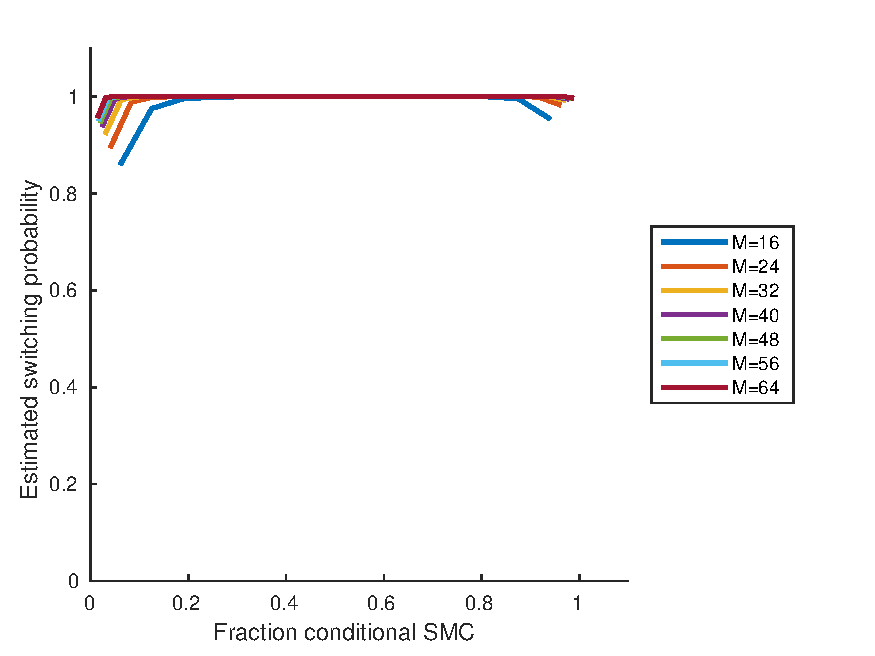
\includegraphics[width=\textwidth,trim={0.3cm 0 0.9cm 0},clip]{Sigma1}
		\caption{$\sigma=1$}
	\end{subfigure}
	~~ %add desired spacing between images, e. g. ~, \quad, \qquad, \hfill etc. 
	%(or a blank line to force the subfigure onto a new line)
	\begin{subfigure}[b]{0.48\textwidth}
		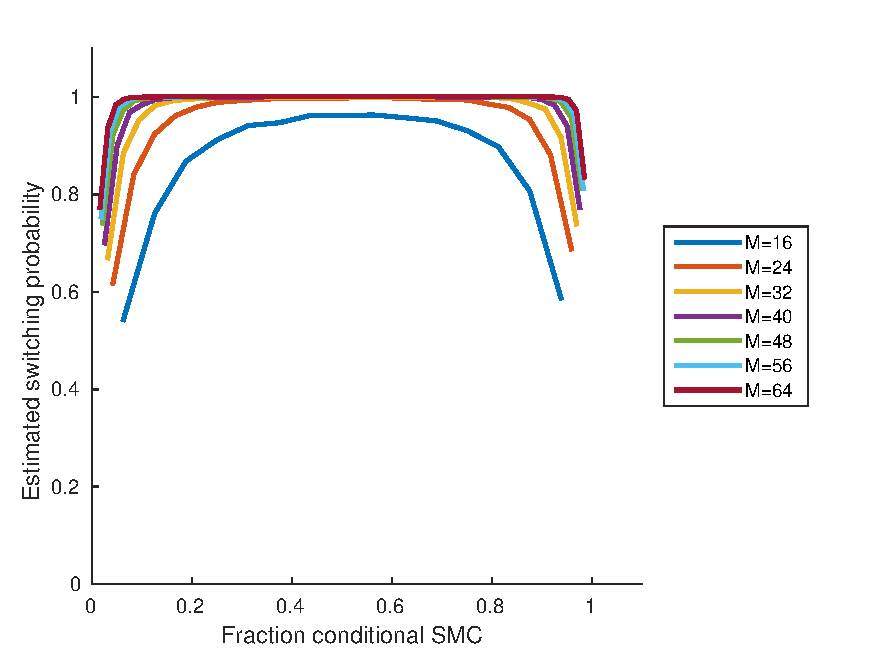
\includegraphics[width=\textwidth,trim={0.3cm 0 0.9cm 0},clip]{Sigma2}
		\caption{$\sigma=2$}
	\end{subfigure}
	
	\begin{subfigure}[b]{0.48\textwidth}
		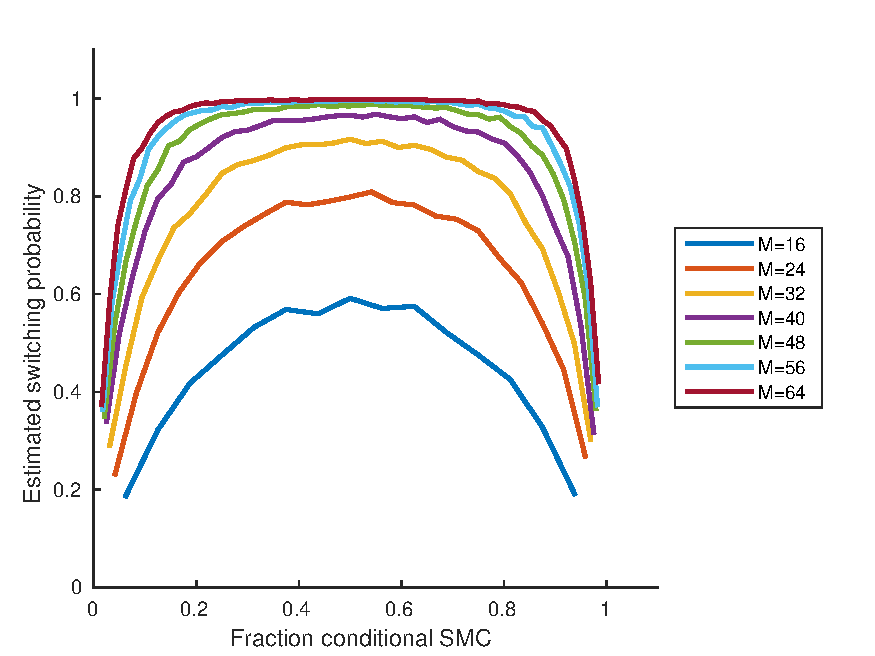
\includegraphics[width=\textwidth,trim={0.3cm 0 0.9cm 0},clip]{Sigma3}
		\caption{$\sigma=3$}
	\end{subfigure}
	~~ %add desired spacing between images, e. g. ~, \quad, \qquad, \hfill etc. 
	%(or a blank line to force the subfigure onto a new line)
	\begin{subfigure}[b]{0.48\textwidth}
		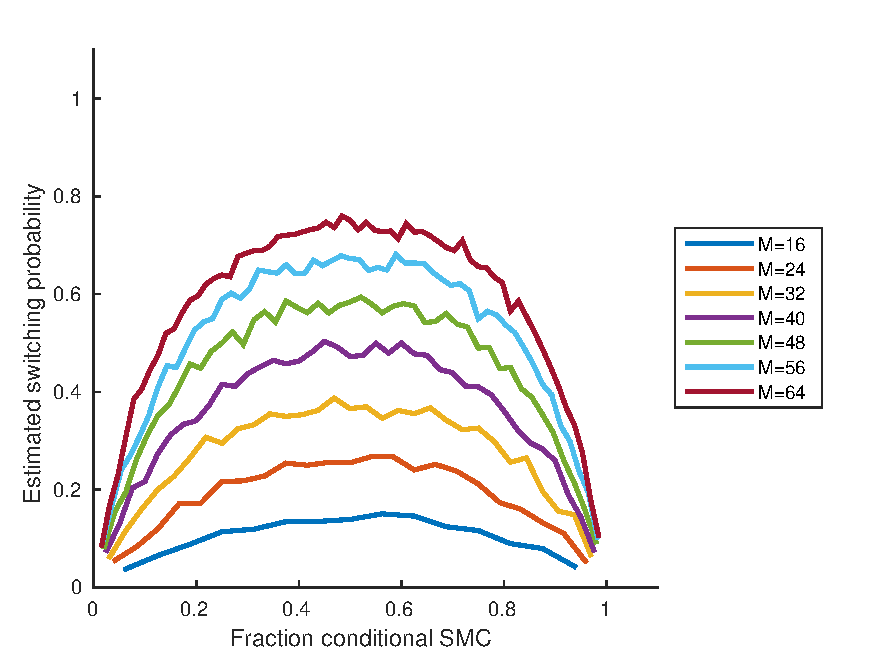
\includegraphics[width=\textwidth,trim={0.3cm 0 0.9cm 0},clip]{Sigma4}
		\caption{$\sigma=4$}
	\end{subfigure}
	
	\begin{subfigure}[b]{0.48\textwidth}
		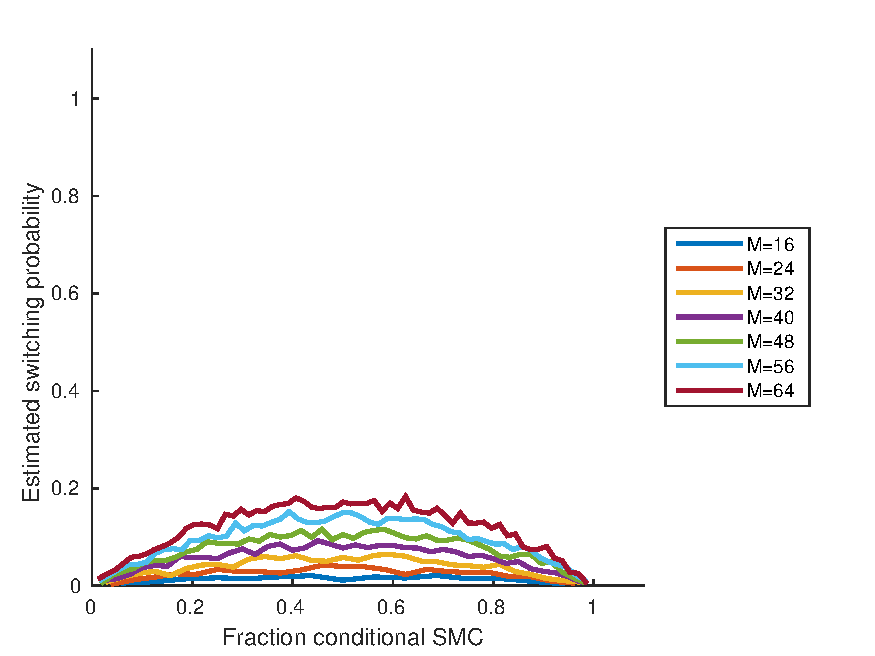
\includegraphics[width=\textwidth,trim={0.3cm 0 0.9cm 0},clip]{Sigma5}
		\caption{$\sigma=5$}
	\end{subfigure}
	~~ %add desired spacing between images, e. g. ~, \quad, \qquad, \hfill etc. 
	%(or a blank line to force the subfigure onto a new line)
	\begin{subfigure}[b]{0.48\textwidth}
		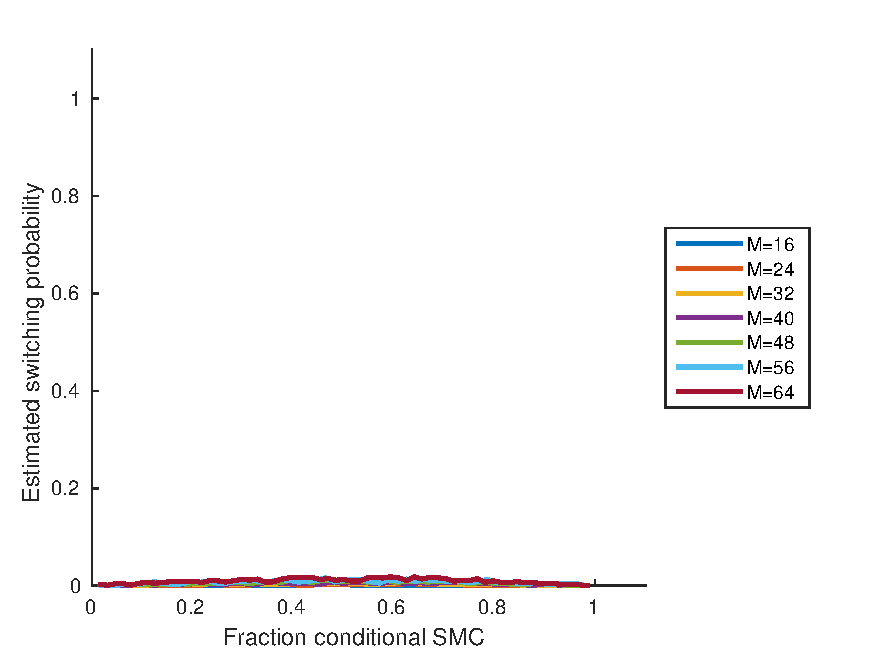
\includegraphics[width=\textwidth,trim={0.3cm 0 0.9cm 0},clip]{Sigma6}
		\caption{$\sigma=6$}
	\end{subfigure}
	\caption{Estimation of switching probability for various settings of $\sigma$ and $M$.}\label{fig:supp-expectedswitch}
\end{figure}

%The crucial quantity in \eqref{eq:switchingprob} is the expectation with respect to all the random variables. By a slight change in notation, \ie by setting $Z_i \eqdef \hat Z_{\pi_T}^i$, we get
%\begin{align}
%\label{eq:condexp}
%\E\left[\prod_{j=1}^P \frac{Z_j}{Z_j +\sum_{i=P+1}^M Z_i}\right] = \E_{Z_{P+1:M}}\left[ \prod_{j=1}^P \int \frac{z_j}{z_j +\sum_{i=P+1}^M Z_i} p(z_j) \myd z_j\right],
%\end{align}
%where $p(z) = \frac{1}{z\sqrt{2\pi \sigma^2}} \exp{\left(-\frac{1}{2\sigma^2}\left(\log z - \frac{\sigma^2}{2}\right)^2\right)}$ for the conditional \smc methods according to the assumption above. Since these are all identically distributed it is enough that we start by considering the following integral
%\begin{align}
%\int \frac{z}{z +a} p(z) \myd z,
%\end{align}
%where we let $a\eqdef\sum_{i=P+1}^M Z_i$ for convenience.

%\begin{align}
%\int \frac{z}{z +a} p(z) \myd z &\leq \int g_a(z) p(z) \myd z = \frac{1}{a}\int_0^a zp(z)\myd z + \int_a^\infty p(z) \myd z =  \frac{1}{a}\int_0^a zp(z)\myd z + \Prb(Z \geq a) \nonumber\\
%&= \frac{1}{a}\int_0^a zp(z)\myd z + 1-\Phi\left(\frac{\log a - \frac{\sigma^2}{2}}{\sigma}\right)%= \left(1-\frac{1}{a}\right)\Prb(Z \geq a) + \frac{1}{a}\E[Z],
%\end{align}
%where $g_a(z) = a^{-1}z, ~0\leq z \leq a$ and $g_a(z) = 1$ otherwise.

%This gives us
%\begin{align*}
%\int \frac{z}{z +a} p(z) \myd z \leq \left(1-\frac{1}{a}\right)\left(1-\Phi\left(\frac{\log a - \frac{\sigma^2}{2}}{\sigma}\right)\right) + \frac{1}{a} e^{\sigma^2} \defeq f(a).
%\end{align*}
%By using the above expression and \eqref{eq:condexp} we can show the following
%\begin{align}
%\label{eq:condexpInequality}
%\E\left[\prod_{j=1}^P \frac{Z_j}{Z_j +\sum_{i=P+1}^M Z_i}\right] \leq \E_{Z_{P+1:M}}\left[ f\left(\sum_{i=P+1}^M Z_i\right)^P\right].
%\end{align}




%From this we can run a Gibbs sampler by first sampling which workers will be the next to retain particles
%\begin{align}
%\label{eq:nodeJoint}
%\tilde \pi(J_P|\xb_{1:M}^{1:N}, \ab_{1:M}^{1:N}) = \frac{\prod_{j=1}^P \hat Z_{\pi_T}^{J_P(j)} \mathbbm{1}_{J_P(j) \neq J_P(1:j-1)}}{\sum_{J_P \in [M]^{\otimes P}} \prod_{m=1}^P \hat Z_{\pi_T}^{J_P(m)} \mathbbm{1}_{J_P(m) \neq J_P(1:m-1)}}.
%\end{align}
%I HAVE THE PROOF FOR THIS AND THAT Z IS THAT AS IF THE RUN WERE A SMC RUN RATHER THAN THE MARGINAL WEIGHT OF THE PARTICLES.  NEED TO WRITE IT UP

%Note that normally this is a $\mathcal{O}(M^P)$ operation, but can be done significantly faster using the method derived in section \ref{sec:SamplingNode}. The next step is to sample the retained particles
%\begin{align*}
%\tilde \pi(K_P|\xb_{1:M}^{1:N}, \ab_{1:M}^{1:N}, J_P) = \prod_{j =1 }^P \frac{w_T(\xb_{J_P(j)}^{K_P(j)})}{\sum_{i=1}^N w_T(\xb_{J_P(j)}^i)},
%\end{align*}
%or by running a backward sampler for better results. Finally, the \smc and \csmc algorithms are run:
%\begin{align*}
%&\tilde \pi(\xb_{1:M}^{1:N}, \ab_{1:M}^{1:N} \backslash \{\xb_{J_P(j)}^{K_P(j)}, \ab_{J_P(j)}^{K_P(j)}\}_{j=1}^P | \{\xb_{J_P(j)}^{K_P(j)}, \ab_{J_P(j)}^{K_P(j)}\}_{j=1}^P, J_P, K_P)\\
%&= \prod_{m=1,m\notin J_P}^M \bar q_{\text{SMC}}\left(\xb_m^{1:N},\ab_m^{1:N}\right) \times \prod_{j = 1}^P \bar q_{\text{CSMC}}\left(\xb_{J_P(j)}^{1:N},\ab_{J_P(j)}^{1:N} \backslash \{\xb_{J_P(j)}^{K_P(j)}, \ab_{J_P(j)}^{K_P(j)}\} \mid \xb_{J_P(j)}^{K_P(j)}, \ab_{J_P(j)}^{K_P(j)}, J_P(j), K_P(j) \right),
%\end{align*}
%\ie we simply run $M-P$ standard independent \smc methods and $P$ \csmc methods.

%Note that $P=M$ essentially reduces to $M$ independent \csmc algorithms and $P=1$ becomes the algorithm we implemented in Anglican during my visit. My guess is that the number of \csmc algorithms should be fairly small compared to the number of independent \smc. - TOM: I think it is actually the other way around in general as the more \csmc then the more particles can be retained and the more "memory" the system has in terms of having nodes converging the true distribution while the \smc nodes are still operating without information gained from previous simulation.  The job of the \smc seems to be more to stop the \csmc getting "stuck".

%Furthermore, I quickly discussed with Fredrik regarding having just the \csmc algorithms run synchronous and the \smc algorithms totally asynchronous, which we felt might work. This means that at each iteration for the \csmc algorithms, they consider whatever amount of independent \smc methods that have already finished. The total number $M$, \ie not $P$ which is still fix, would be random number.

%\subsection{Derivation Details Based on Extended Target}
%Here we provide the details on how we derive the conditionals to simulate from based on \eqref{eq:dmc-smc} above. Let us start by re-writing \eqref{eq:dmc-smc}
%\begin{align*}
%&\tilde \pi(\xb_{1:M}^{1:N}, \ab_{1:M}^{1:N}, J_P, K_P) = \frac{1}{\binom{M}{P}} \prod_{m=1}^M \bar q_{\text{SMC}}\left(\xb_m^{1:N},\ab_m^{1:N}\right)  \times \prod_{j = 1}^P \mathbbm{1}_{J_P(j) \neq J_P(1:j-1)} \frac{w_T(\xb_{J_P(j)}^{K_P(j)})}{\sum_{i=1}^N w_T(\xb_{J_P(j)}^i)}  \\
%&\times \prod_{j = 1}^P \bar\pi_T\left(\xb_{J_P(j)}^{K_P(j)}\right) \frac{\bar q_{\text{CSMC}}\left(\xb_{J_P(j)}^{1:N},\ab_{J_P(j)}^{1:N} \backslash \{\xb_{J_P(j)}^{K_P(j)}, \ab_{J_P(j)}^{K_P(j)}\} \mid \xb_{J_P(j)}^{K_P(j)}, \ab_{J_P(j)}^{K_P(j)}, J_P(j), K_P(j) \right)}{N^{T} \frac{w_T(\xb_{J_P(j)}^{K_P(j)})}{\sum_{i=1}^N w_T(\xb_{J_P(j)}^i)} \bar q_{\text{SMC}}\left(\xb_{J_P(j)}^{1:N},\ab_{J_P(j)}^{1:N}\right)}\\
%&= \frac{1}{\binom{M}{P}} \prod_{m=1}^M \bar q_{\text{SMC}}\left(\xb_m^{1:N},\ab_m^{1:N}\right)  \times \prod_{j = 1}^P \frac{\hat Z_{\pi_T}^{J_P(j)}}{Z_{\pi_T}}\mathbbm{1}_{J_P(j) \neq J_P(1:j-1)} \frac{w_T(\xb_{J_P(j)}^{K_P(j)})}{\sum_{i=1}^N w_T(\xb_{J_P(j)}^i)}.
%\end{align*}
%%\cnnote{Double-check the above re-write!}

%Now, by first marginalising over $K_P$ we get
%\begin{align*}
%&\tilde \pi(\xb_{1:M}^{1:N}, \ab_{1:M}^{1:N}, J_P) = \frac{1}{\binom{M}{P}} \prod_{m=1}^M \bar q_{\text{SMC}}\left(\xb_m^{1:N},\ab_m^{1:N}\right)  \times \prod_{j = 1}^P \frac{\hat Z_{\pi_T}^{J_P(j)}}{Z_{\pi_T}}\mathbbm{1}_{J_P(j) \neq J_P(1:j-1)},
%\end{align*}
%and thus to sample $J_P$ (the worker indices with retained particles) we simulate from
%\begin{align*}
%&\tilde \pi(J_P \mid \xb_{1:M}^{1:N}, \ab_{1:M}^{1:N}) \propto \prod_{j = 1}^P \hat Z_{\pi_T}^{J_P(j)} \mathbbm{1}_{J_P(j) \neq J_P(1:j-1)}.
%\end{align*}
%How this can be done efficiently is detailed in section \ref{sec:SamplingNode}.  Then to simulate the corresponding retained particles
%\begin{align*}
%&\tilde \pi(K_P \mid \xb_{1:M}^{1:N}, \ab_{1:M}^{1:N}, J_P) = \prod_{j = 1}^P \frac{w_T(\xb_{J_P(j)}^{K_P(j)})}{\sum_{i=1}^N w_T(\xb_{J_P(j)}^i)},
%\end{align*}
%and finally given these we can run the \smc and \csmc algorithms
%\begin{align*}
%&\tilde \pi(\xb_{1:M}^{1:N}, \ab_{1:M}^{1:N} \backslash \{\xb_{J_P(j)}^{K_P(j)}, \ab_{J_P(j)}^{K_P(j)}\}_{j=1}^P | \{\xb_{J_P(j)}^{K_P(j)}, \ab_{J_P(j)}^{K_P(j)}\}_{j=1}^P, J_P, K_P)\\
%&= \prod_{m=1,m\notin J_P}^M \bar q_{\text{SMC}}\left(\xb_m^{1:N},\ab_m^{1:N}\right) \times \prod_{j = 1}^P \bar q_{\text{CSMC}}\left(\xb_{J_P(j)}^{1:N},\ab_{J_P(j)}^{1:N} \backslash \{\xb_{J_P(j)}^{K_P(j)}, \ab_{J_P(j)}^{K_P(j)}\} \mid \xb_{J_P(j)}^{K_P(j)}, \ab_{J_P(j)}^{K_P(j)}, J_P(j), K_P(j) \right).
%\end{align*}
%We have now shown that running a (partially collapsed) Gibbs sampler for \eqref{eq:dmc-smc} results in the proposed algorithm. This means our samples $\{\xb_{J_P(j)}^{K_P(j)}, \ab_{J_P(j)}^{K_P(j)}\}_{j=1}^P$ will be marginally distributed as the distribution of interest $\bar \pi_T$! (\ie in stationarity).

%% USING ALL PARTICLES
%\subsection{Using All Particles}
%Typically our estimator for a test function $f$ based on $R$ iterations of the above algorithm would be
%\begin{align}
%\E[f(\xb)] \approx \frac{1}{RP} \sum_{r=1}^R \sum_{j=1}^P f(\xb_{J_P(j)}^{K_P(j)}[r]).
%\end{align}
%However, below we show that we can re-use all the generated particles by marginalising over the indices $J_P$ and $K_P$.
%\begin{align}
%&\E[f(\xb)] \approx \frac{1}{RP} \sum_{r=1}^R \sum_{j=1}^P \E_{J_P}\E_{K_P}\left[ f(\xb_{J_P(j)}^{K_P(j)}[r]) \right] = \frac{1}{RP} \sum_{r=1}^R \sum_{j=1}^P \E_{J_P} \left[ \sum_{i=1}^N \bar w_T(\xb_{J_P(j)}^{i}[r]) f(\xb_{J_P(j)}^{i}[r]) \right] \nonumber \\
%&= \frac{1}{RP} \sum_{r=1}^R \sum_{j=1}^P \E_{J_P(j)} \left[ \sum_{i=1}^N \bar w_T(\xb_{J_P(j)}^{i}[r]) f(\xb_{J_P(j)}^{i}[r]) \right] = \frac{1}{R} \sum_{r=1}^R \E_{J_P(1)} \left[ \sum_{i=1}^N \bar w_T(\xb_{J_P(1)}^{i}[r]) f(\xb_{J_P(1)}^{i}[r]) \right] \nonumber \\
%&= \frac{1}{R} \sum_{r=1}^R \sum_{m=1}^M \beta_m[r] \sum_{i=1}^N \bar w_T(\xb_{m}^{i}[r]) f(\xb_{m}^{i}[r]),
%\end{align}
%where $\bar w_T(\xb_{J_P(j)}^{i}) = \frac{w_T(\xb_{J_P(j)}^{i})}{\sum_{\ell=1}^N w_T(\xb_{J_P(j)}^\ell)}$ and $\beta_m[r]$ is defined as the probability $\tilde\pi(m)$ in \eqref{eq:singleNode} calculated at each iteration $r$.

%Alternative when we sample $J_P$ using a one-at-the-time Gibbs we should probably marginalise as follows instead:
%\begin{align}
%\label{eq:gibbsRB}
%&\E[f(\xb)] \approx \frac{1}{RP} \sum_{r=1}^R \sum_{j=1}^P \E_{J_P(j)|J_P\backslash\{J_P(j)\}}\E_{K_P | J_P}\left[ f(\xb_{J_P(j)}^{K_P(j)}[r]) \right] = \frac{1}{RP} \sum_{r=1}^R \sum_{j=1}^P \E_{J_P(j)|J_P\backslash\{J_P(j)\}} \left[ \sum_{i=1}^N \bar w_T(\xb_{J_P(j)}^{i}[r]) f(\xb_{J_P(j)}^{i}[r]) \right]\nonumber \\
%&  = \frac{1}{RP} \sum_{r=1}^R \sum_{j=1}^P \sum_{m=1}^M \beta_m^j[r] \sum_{i=1}^N \bar w_T(\xb_{m}^{i}[r]) f(\xb_m^{i}[r]) = \frac{1}{R} \sum_{r=1}^R \sum_{m=1}^M \tilde \beta_m[r] \sum_{i=1}^N \bar w_T(\xb_{m}^{i}[r]) f(\xb_m^{i}[r]),
%\end{align}
%where $\beta_m^j[r] = \frac{\hat Z_{\pi_T}^m \mathbbm{1}_{m \neq J_P\backslash \{J_P(j)\}}}{\sum_\ell \hat Z_{\pi_T}^\ell \mathbbm{1}_{\ell \neq J_P\backslash \{J_P(j)\}}}$ for each iteration $r$. The last equality is just a simplification where $\tilde \beta_m[r] = P^{-1}\sum_{j=1}^P \beta_m^j[r] $ is the weights assigned to each node. That means if sample conditional nodes for $j=1,\ldots,P$ like follows
%\begin{align}
%\tilde \pi(J_P(j) \mid J_P\backslash\{J_P(j)\}, \xb_{1:M}^{1:N}, \ab_{1:M}^{1:N}) \propto \hat Z_{\pi_T}^{J_P(j)} \mathbbm{1}_{J_P(j) \neq J_P\backslash\{J_P(j)\}},
%\end{align}
%these probabilities are actually the $\beta_m^j[r]$ that we input above in \eqref{eq:gibbsRB}.

% % % % % % % % % % % % % % % OTHER FIGURES % % % % % % % % % %
\newpage
\section{Additional Results Figures}
\label{sec:supp-additionalFigures}

%In this section we provide figures to support those in the main paper.
\vspace{-10pt}
\begin{figure*}[h!]
	\centering
	\begin{subfigure}[t]{0.48\textwidth}
		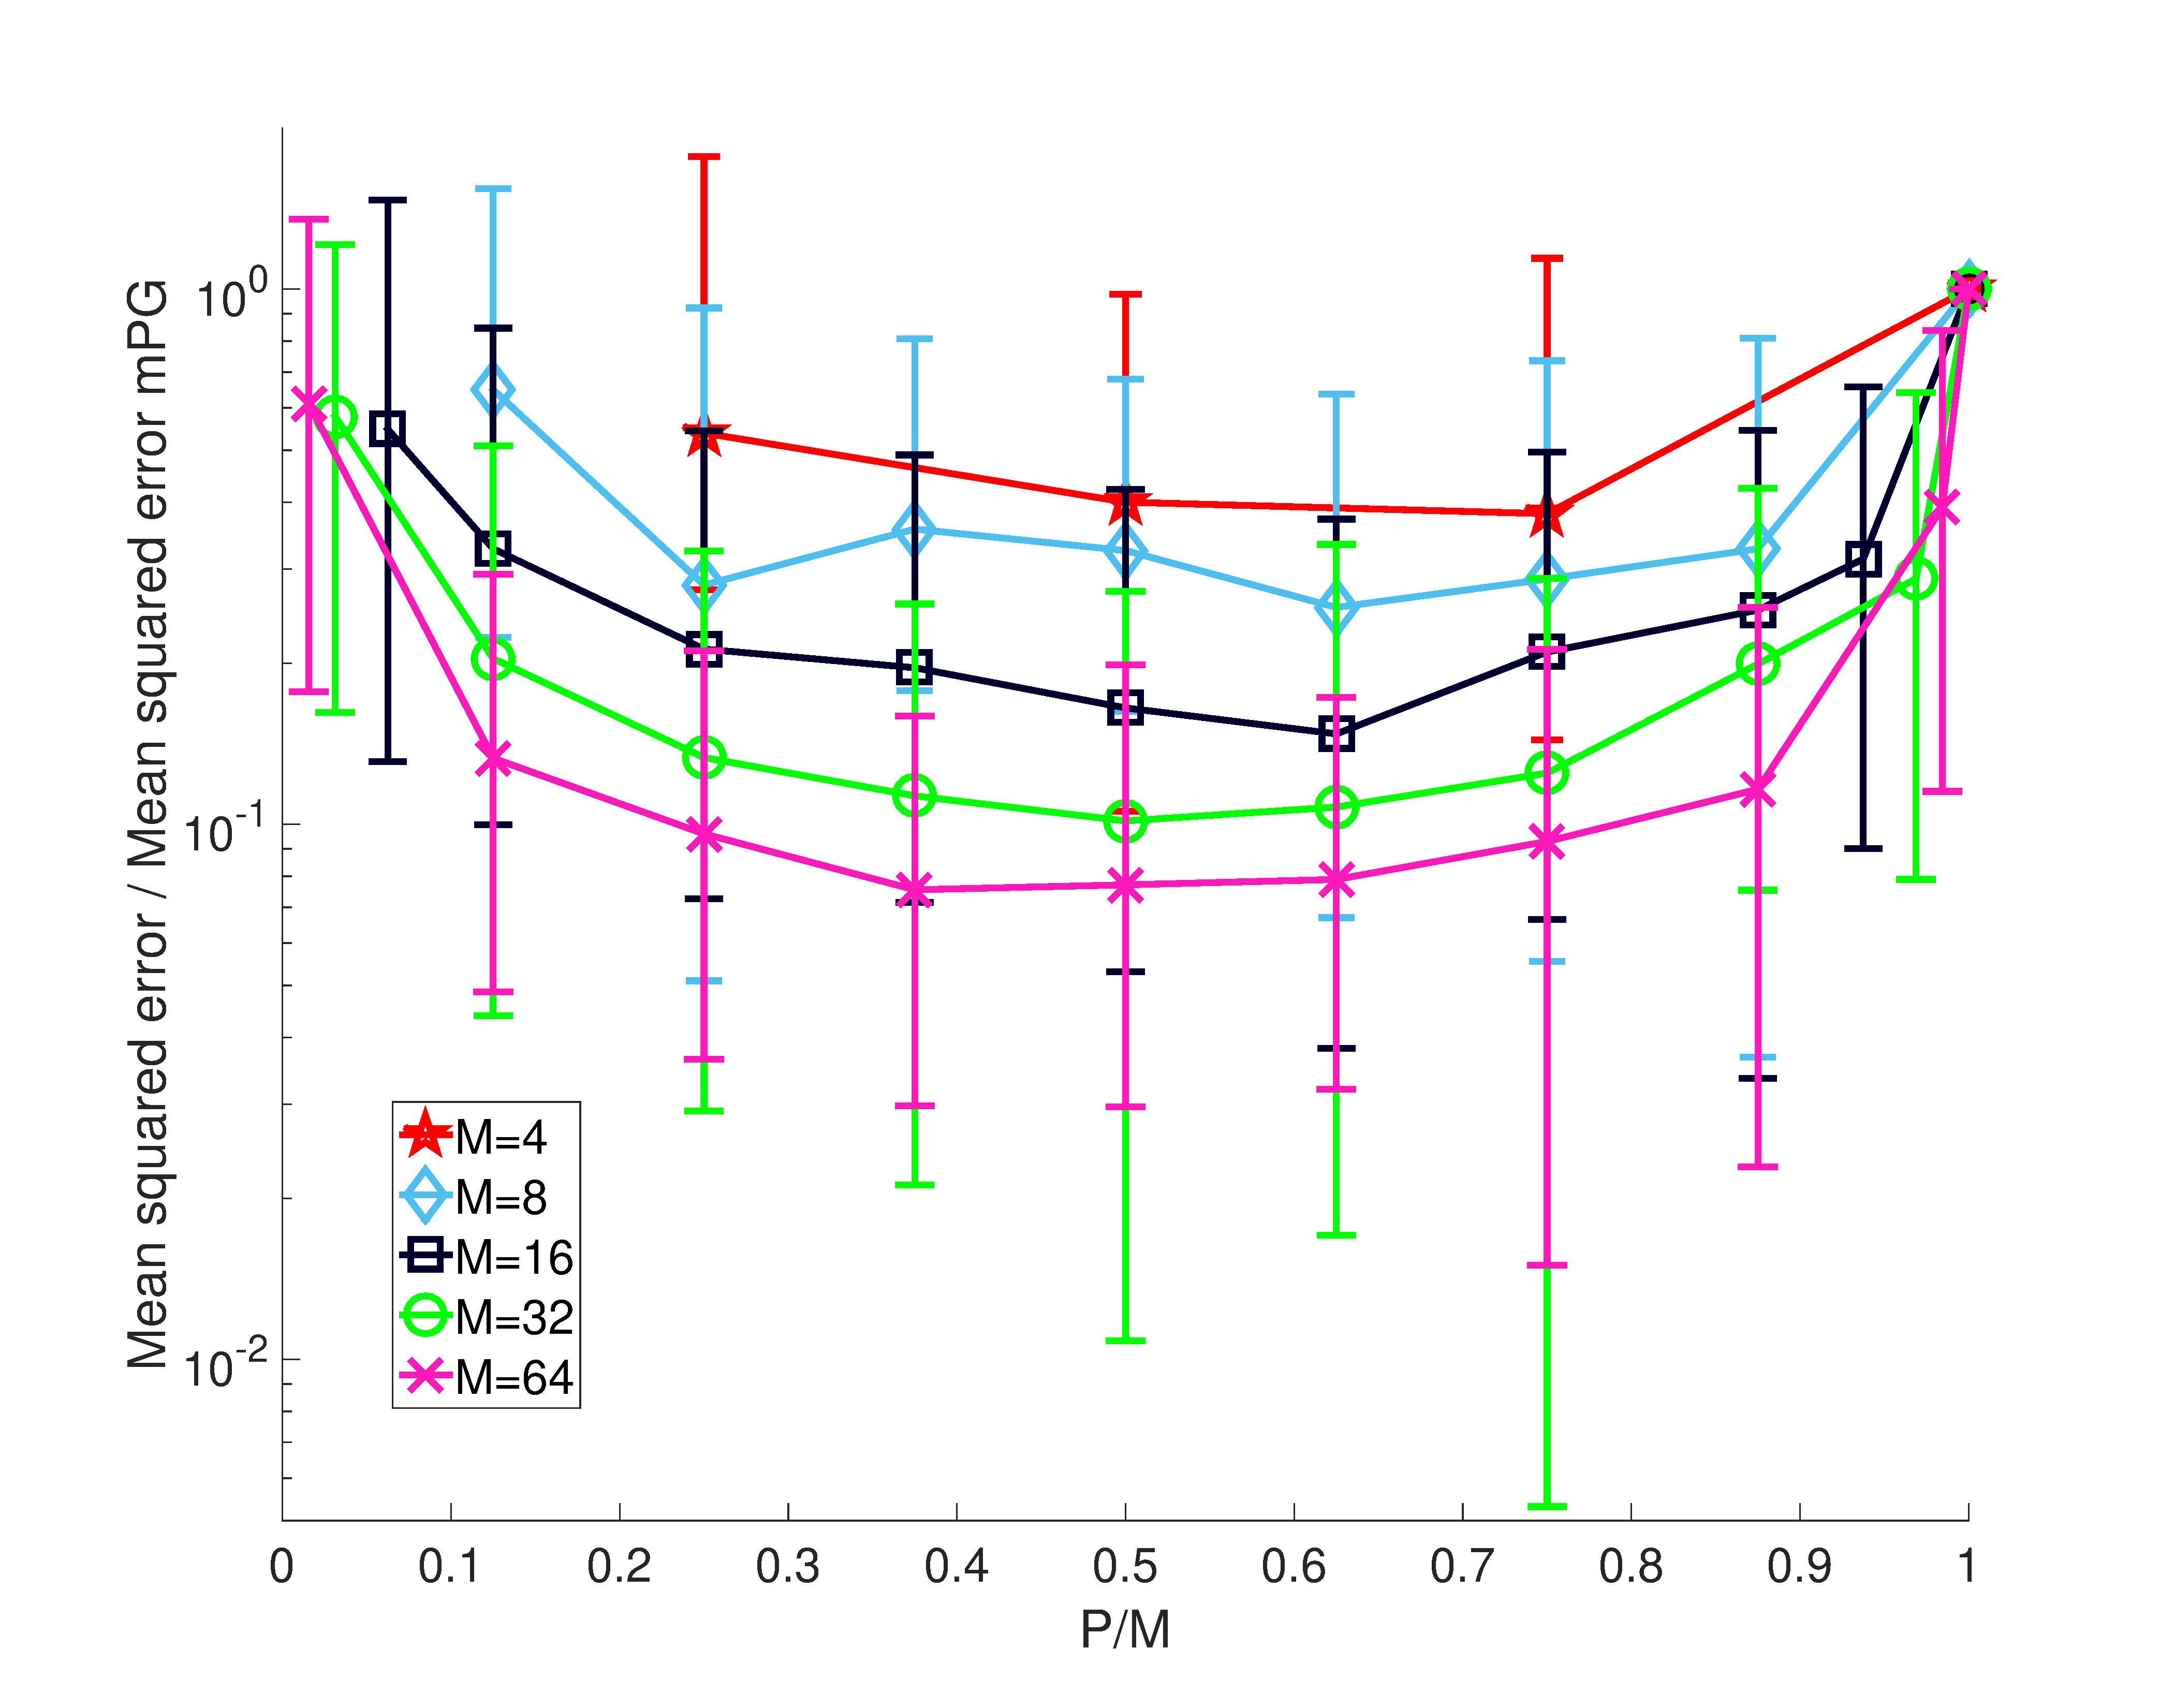
\includegraphics[width=\textwidth,trim={4cm 0 6cm 0},clip]{mean_P_over_M_sweep}
		\caption{Mean}
		\label{fig:supp-meanConv}
	\end{subfigure}
	~~~ %add desired spacing between images, e. g. ~, \quad, \qquad, \hfill etc. 
	%(or a blank line to force the subfigure onto a new line)
	\begin{subfigure}[t]{0.48\textwidth}
		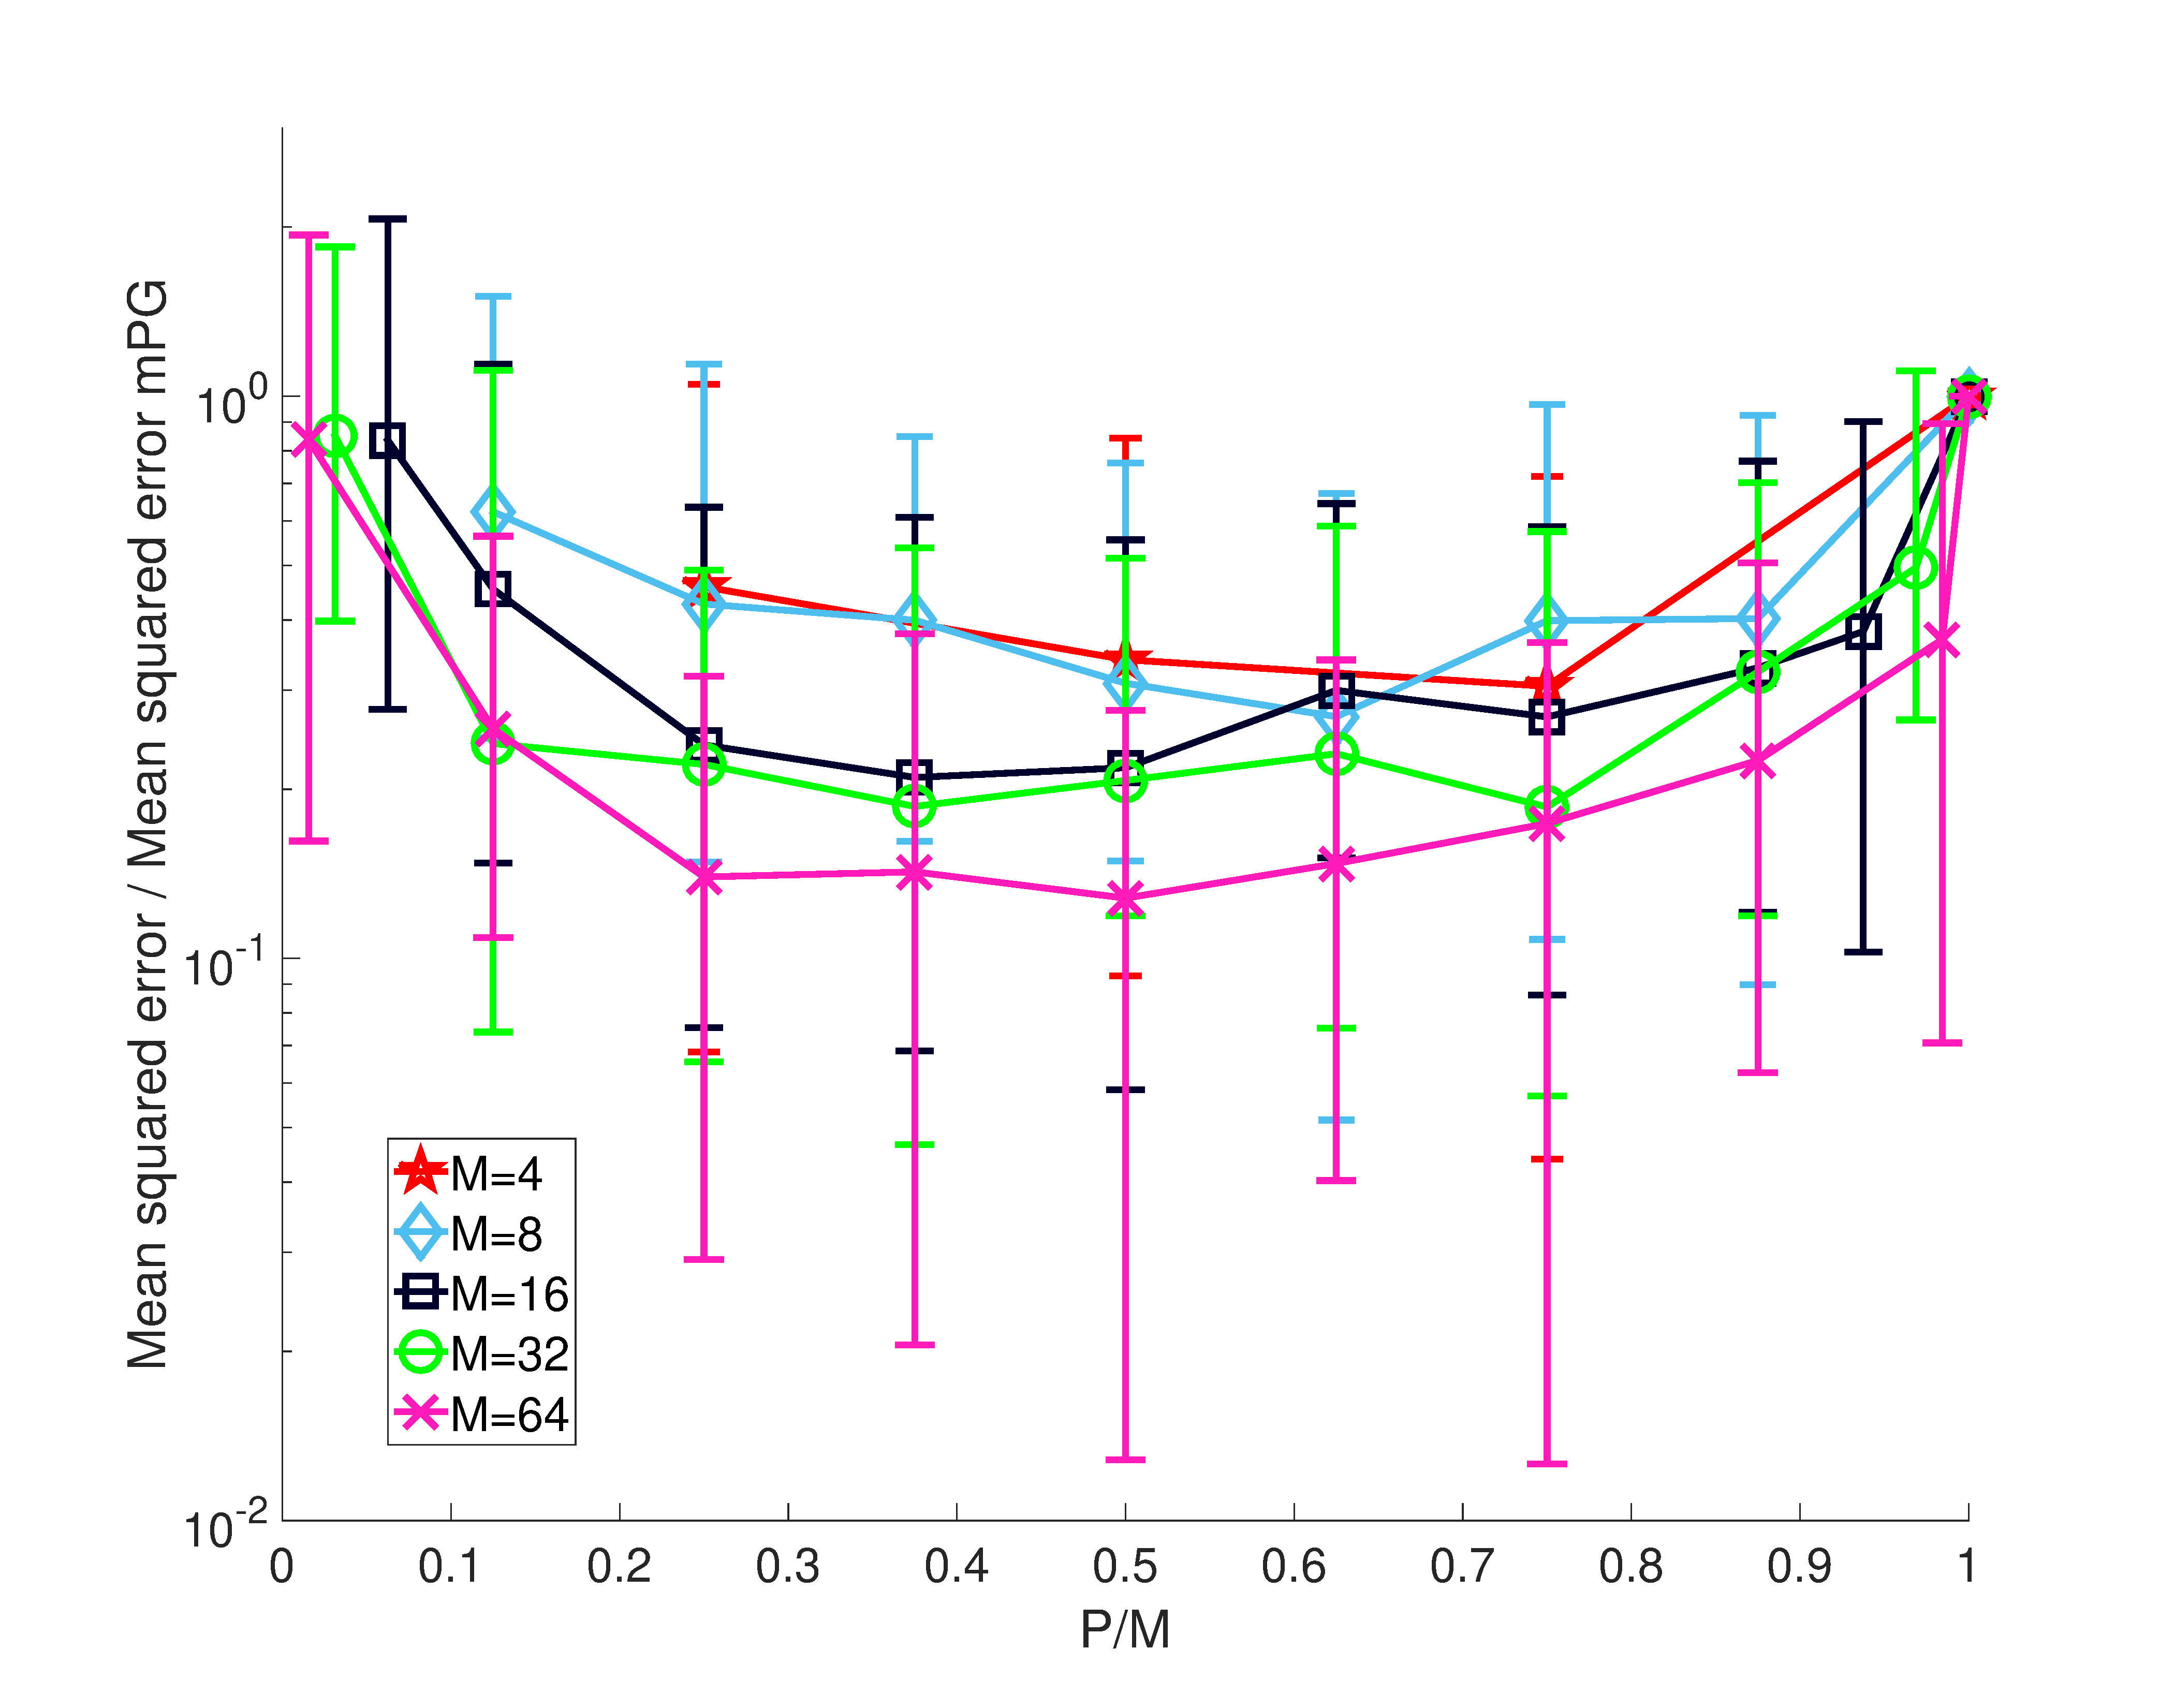
\includegraphics[width=\textwidth,trim={4cm 0 6cm 0},clip]{std_P_over_M_sweep}
		\caption{Standard Deviation}
		\label{fig:supp-meanPos}
	\end{subfigure}
	
	\begin{subfigure}[t]{0.48\textwidth}
		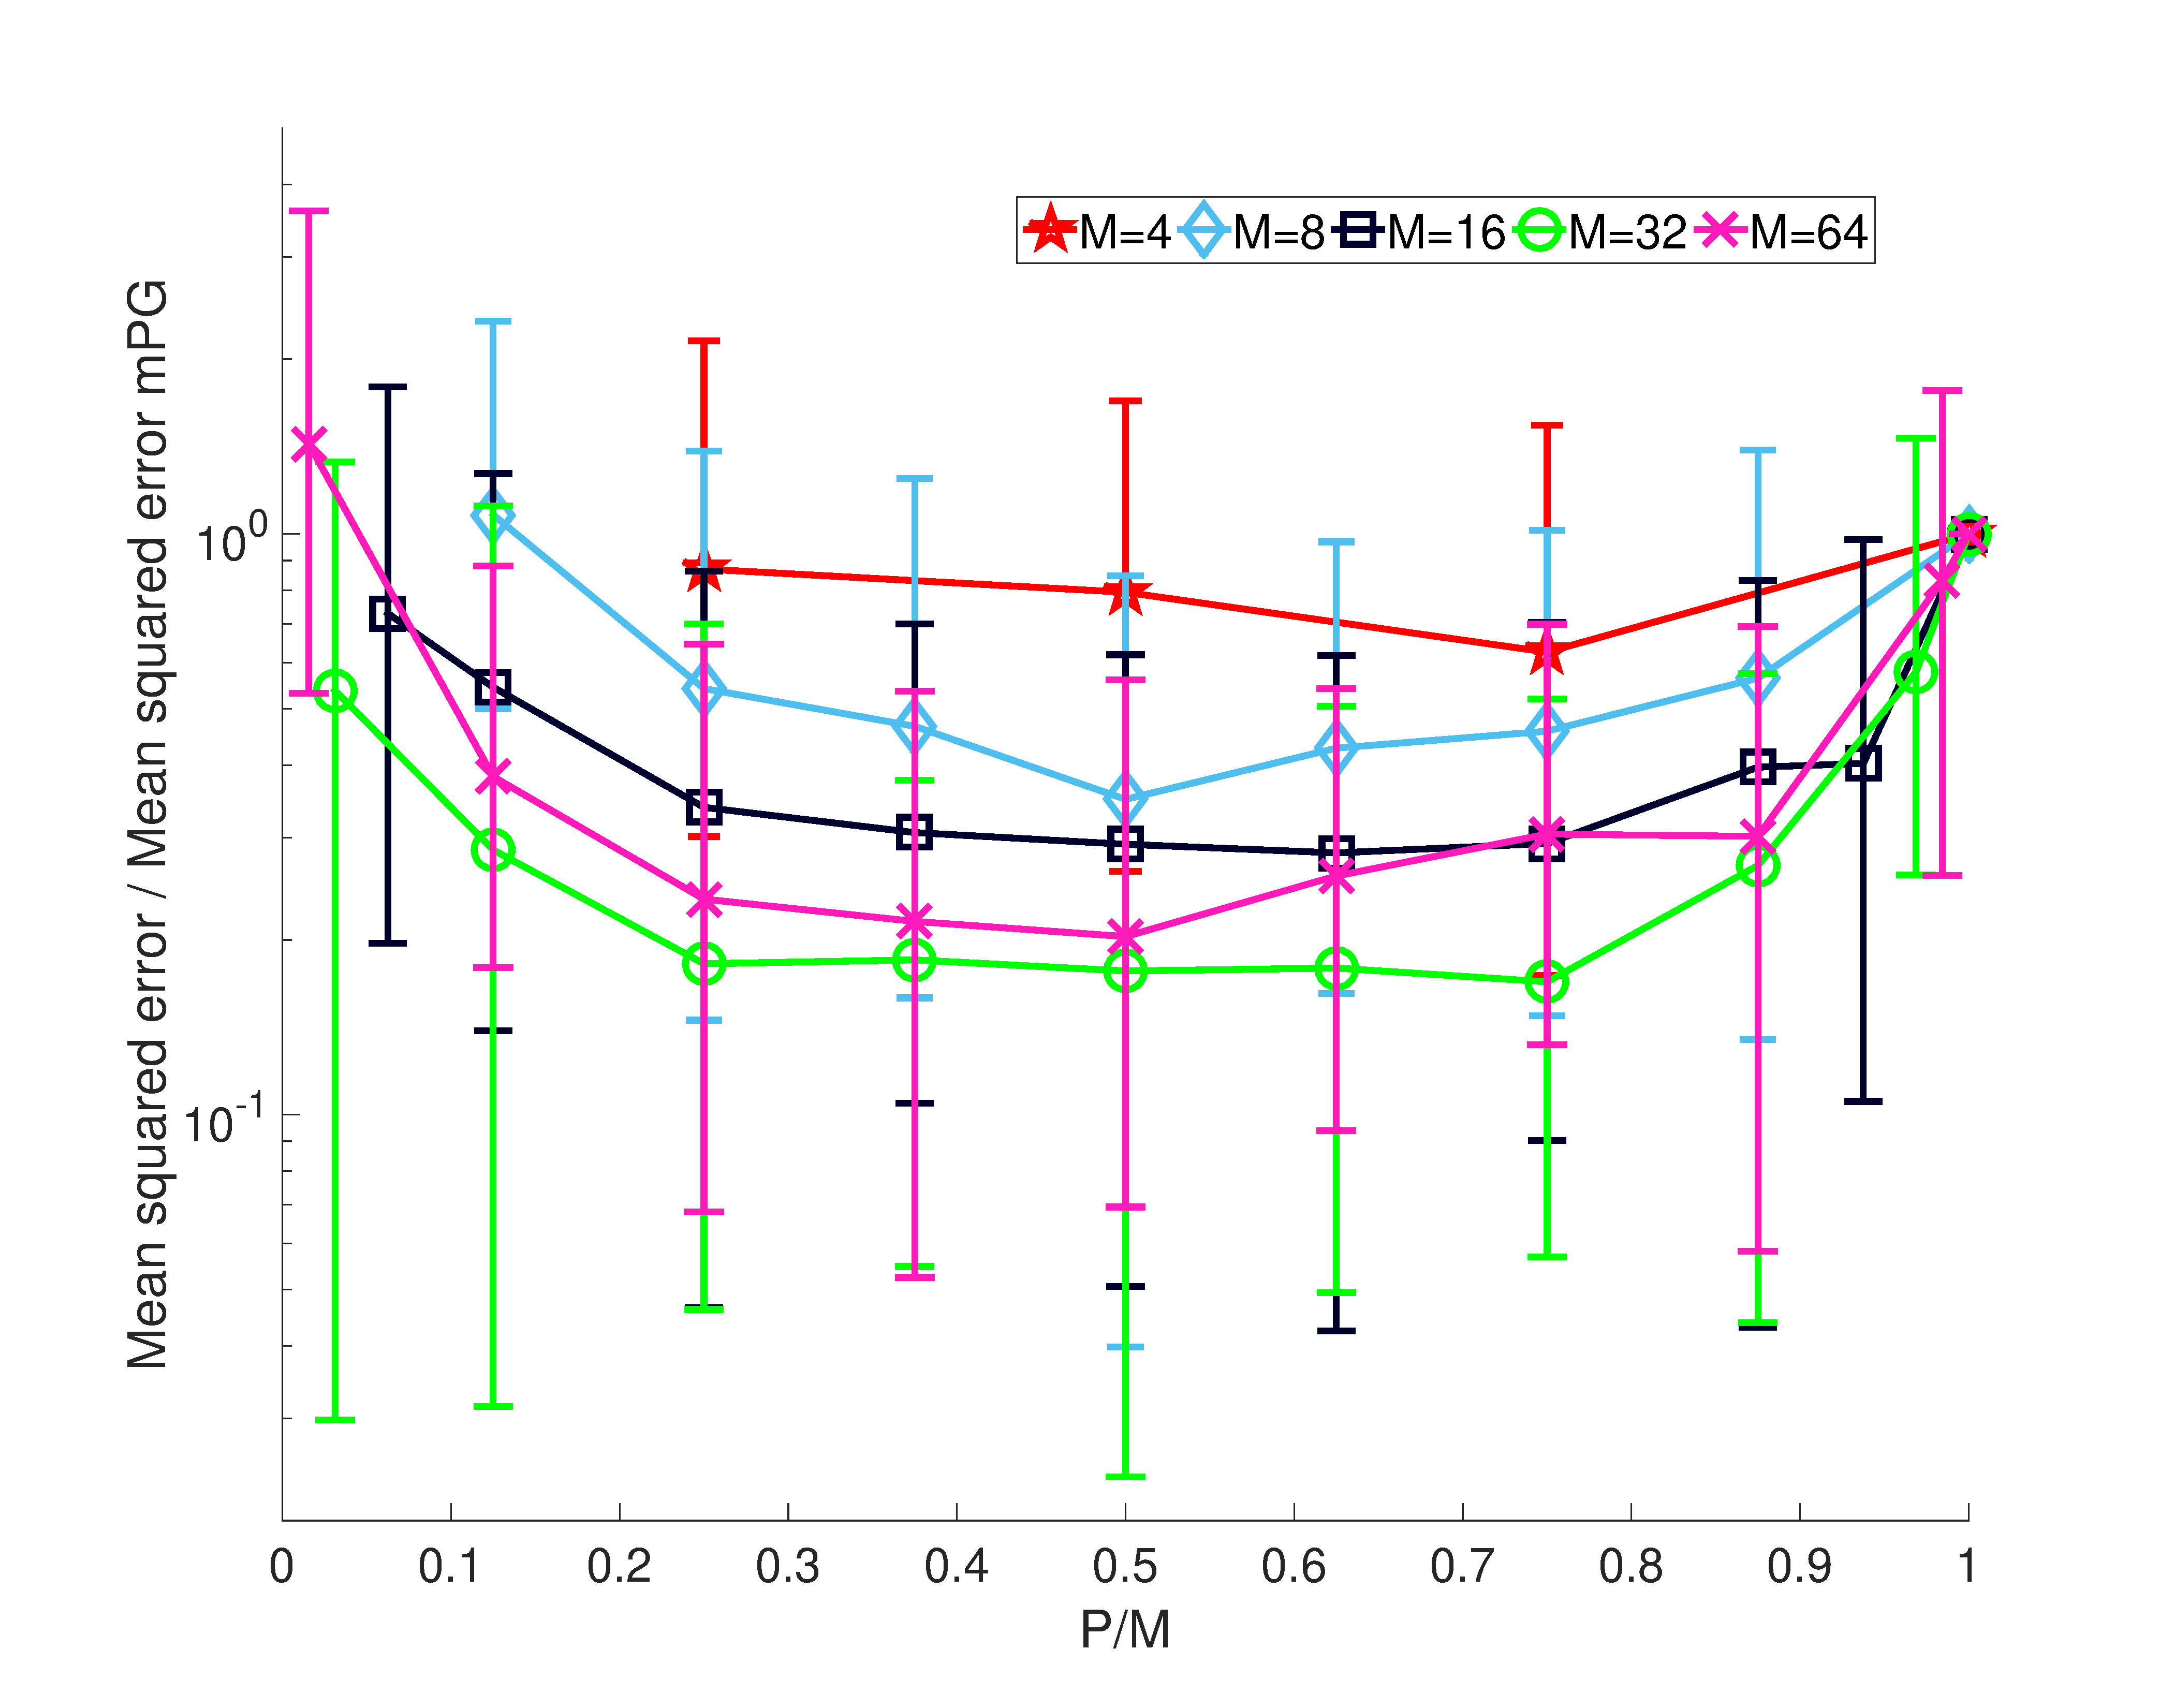
\includegraphics[width=\textwidth,trim={4cm 0 6cm 0},clip]{skewness_P_over_M_sweep}
		\caption{Skewness}
		\label{fig:supp-stdConv}
	\end{subfigure}
	~~~ %add desired spacing between images, e. g. ~, \quad, \qquad, \hfill etc. 
	%(or a blank line to force the subfigure onto a new line)
	\begin{subfigure}[t]{0.48\textwidth}
		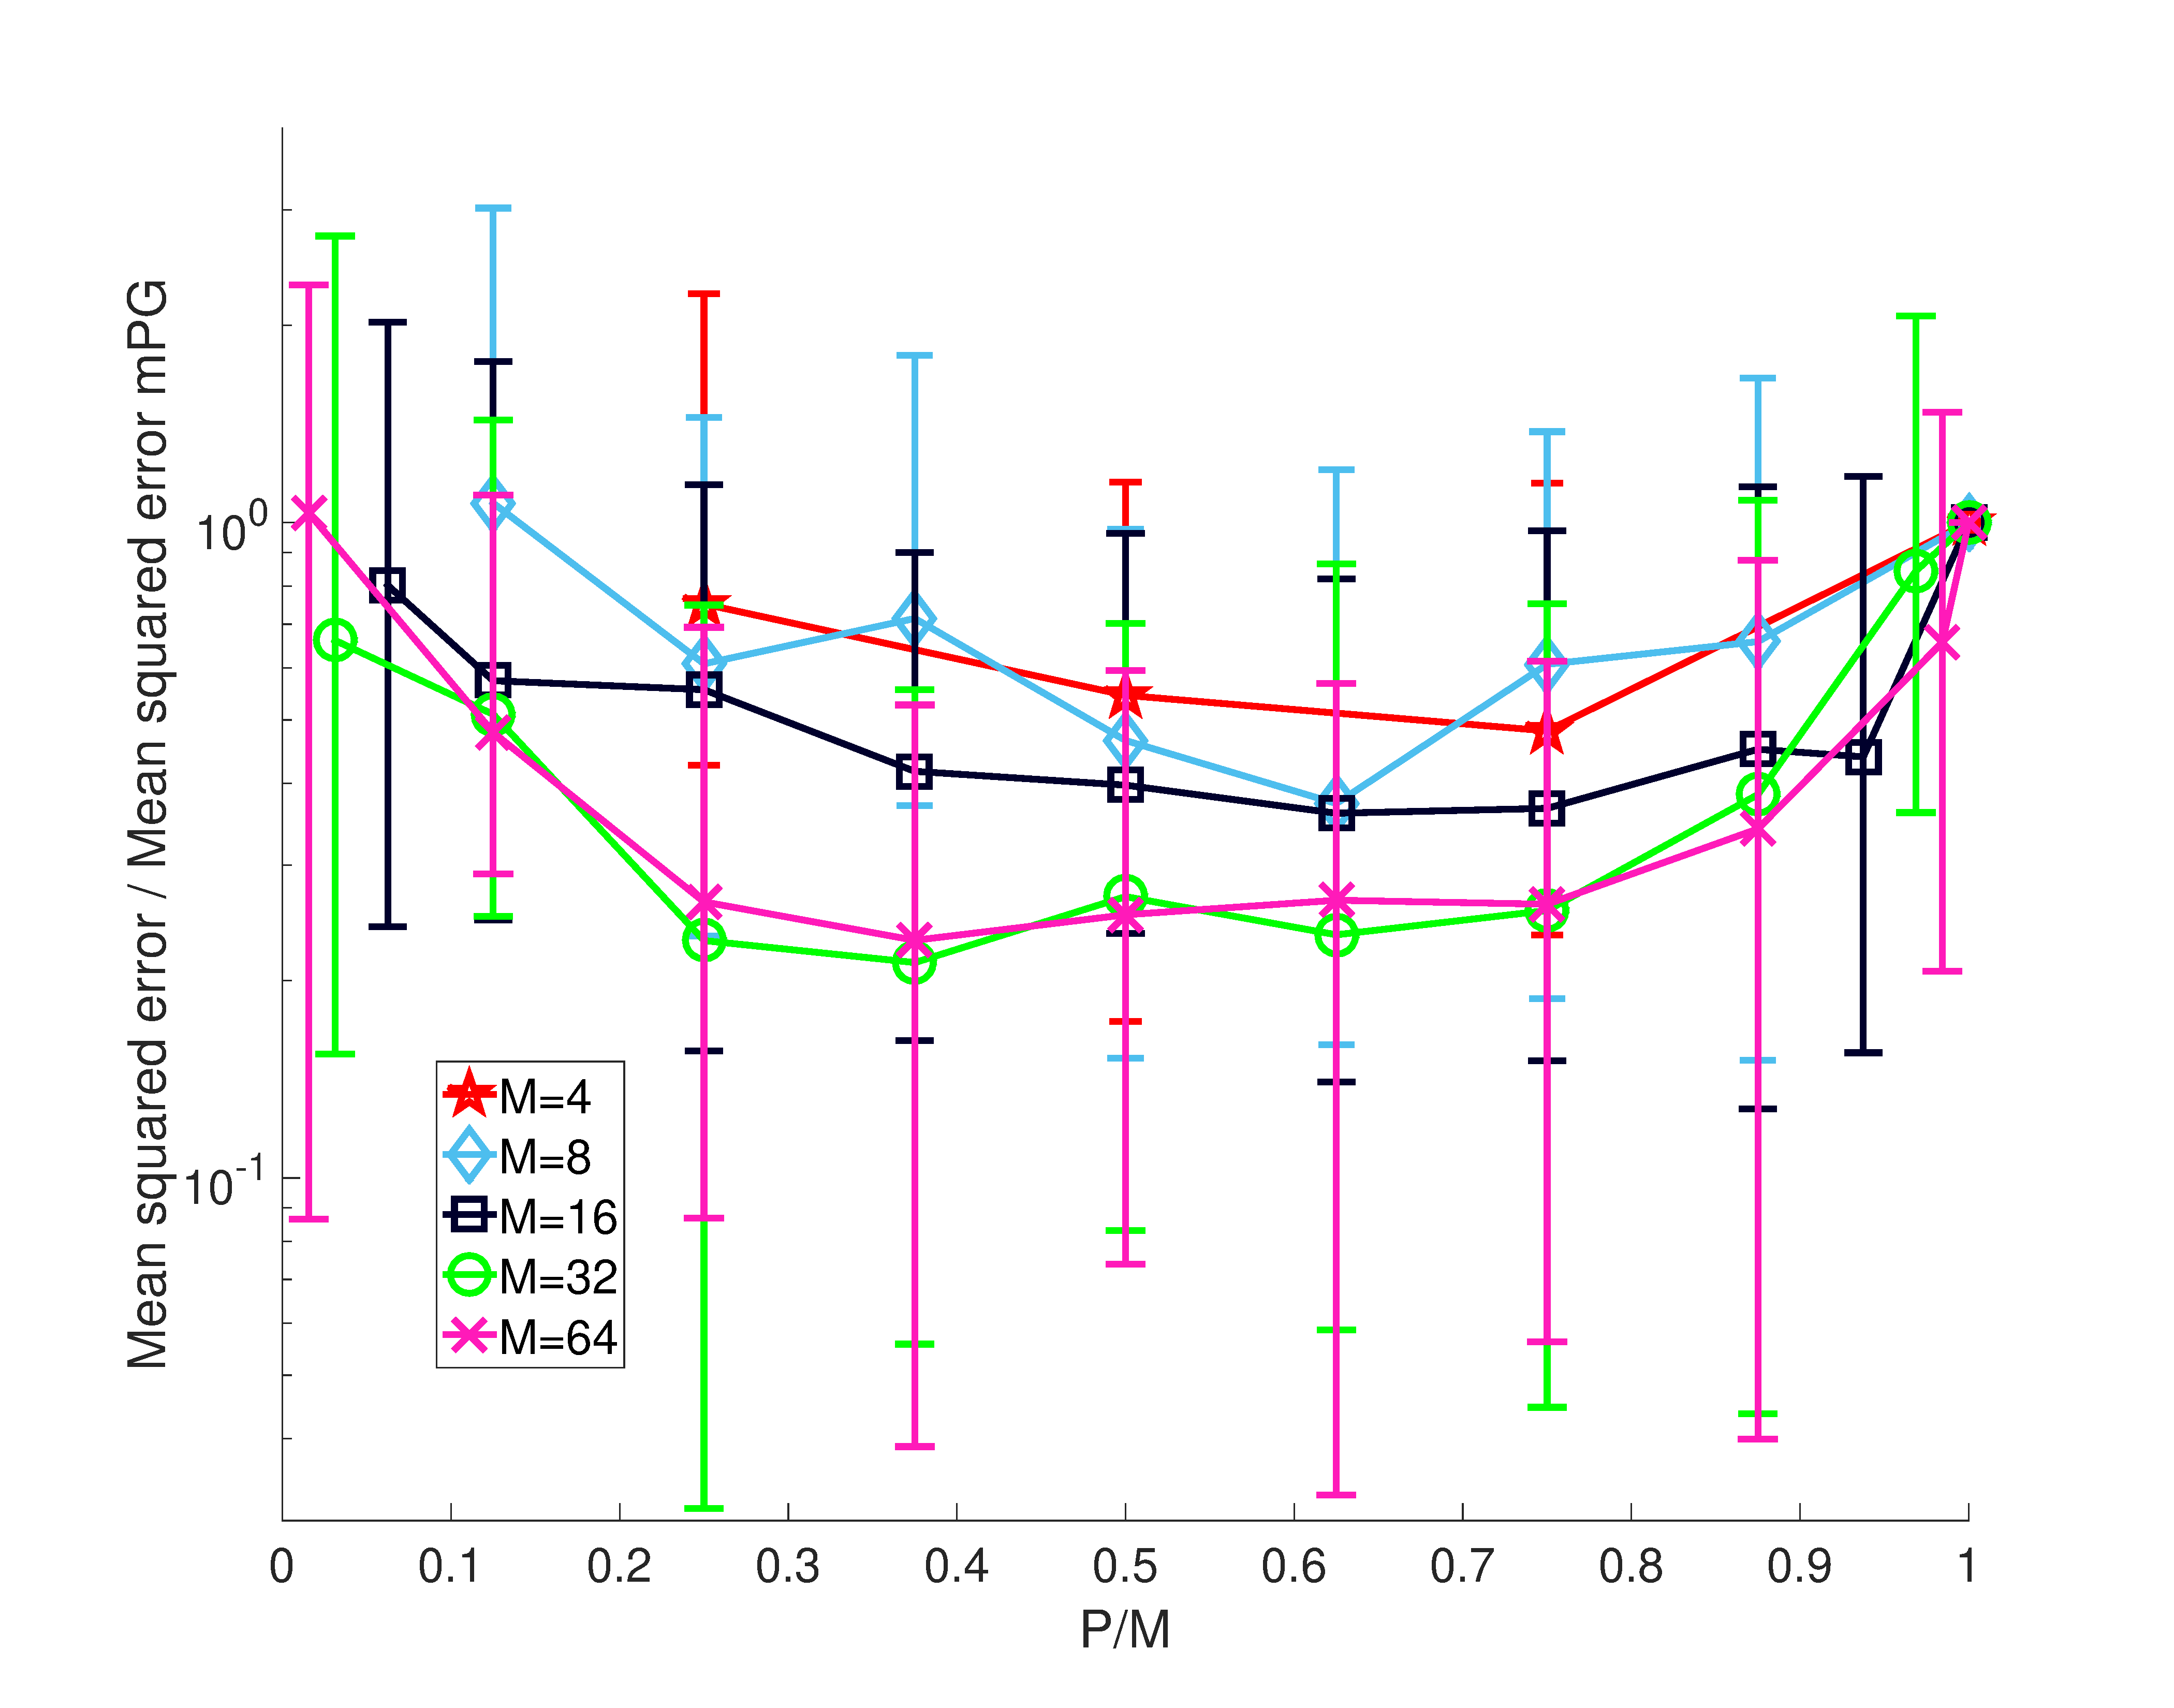
\includegraphics[width=\textwidth,trim={4cm 0 6cm 0},clip]{kurtosis_P_over_M_sweep}
		\caption{Kurtosis}
		\label{fig:supp-stdPos}
	\end{subfigure}	
	\caption{Median error in marginal moment estimates with different choices of P and M over 10 different synthetic datasets of the linear Gaussian state space model given in (10) after 1000 MCMC iterations. Errors are normalized by the error of a multi-start PG sampler which is a special case of iPMCMC for which $P=M$ (see Section 4).  Error bars show the lower and upper quartiles for the errors.  It can be seen that for all the moments then $P/M\approx1/2$ give the best performance. For the mean and standard deviation estimates, the accuracy relative to the non-interacting distribution case $P=M$ shows a clear increase with $M$. This effect is also seen for the skewness and excess kurtosis estimates except for the distinction between the $M=32$ and $M=64$ cases.  This may be because these metric are the same for the prior and the posterior such that good results for these metric might be achievable even when the samples give a poor match to the true posterior. \label{fig:supp-pSweepErrorBar}}
\end{figure*}

\begin{figure*}[p]
	\centering
	\begin{subfigure}[t]{0.49\textwidth}
		\makebox[\textwidth][r]{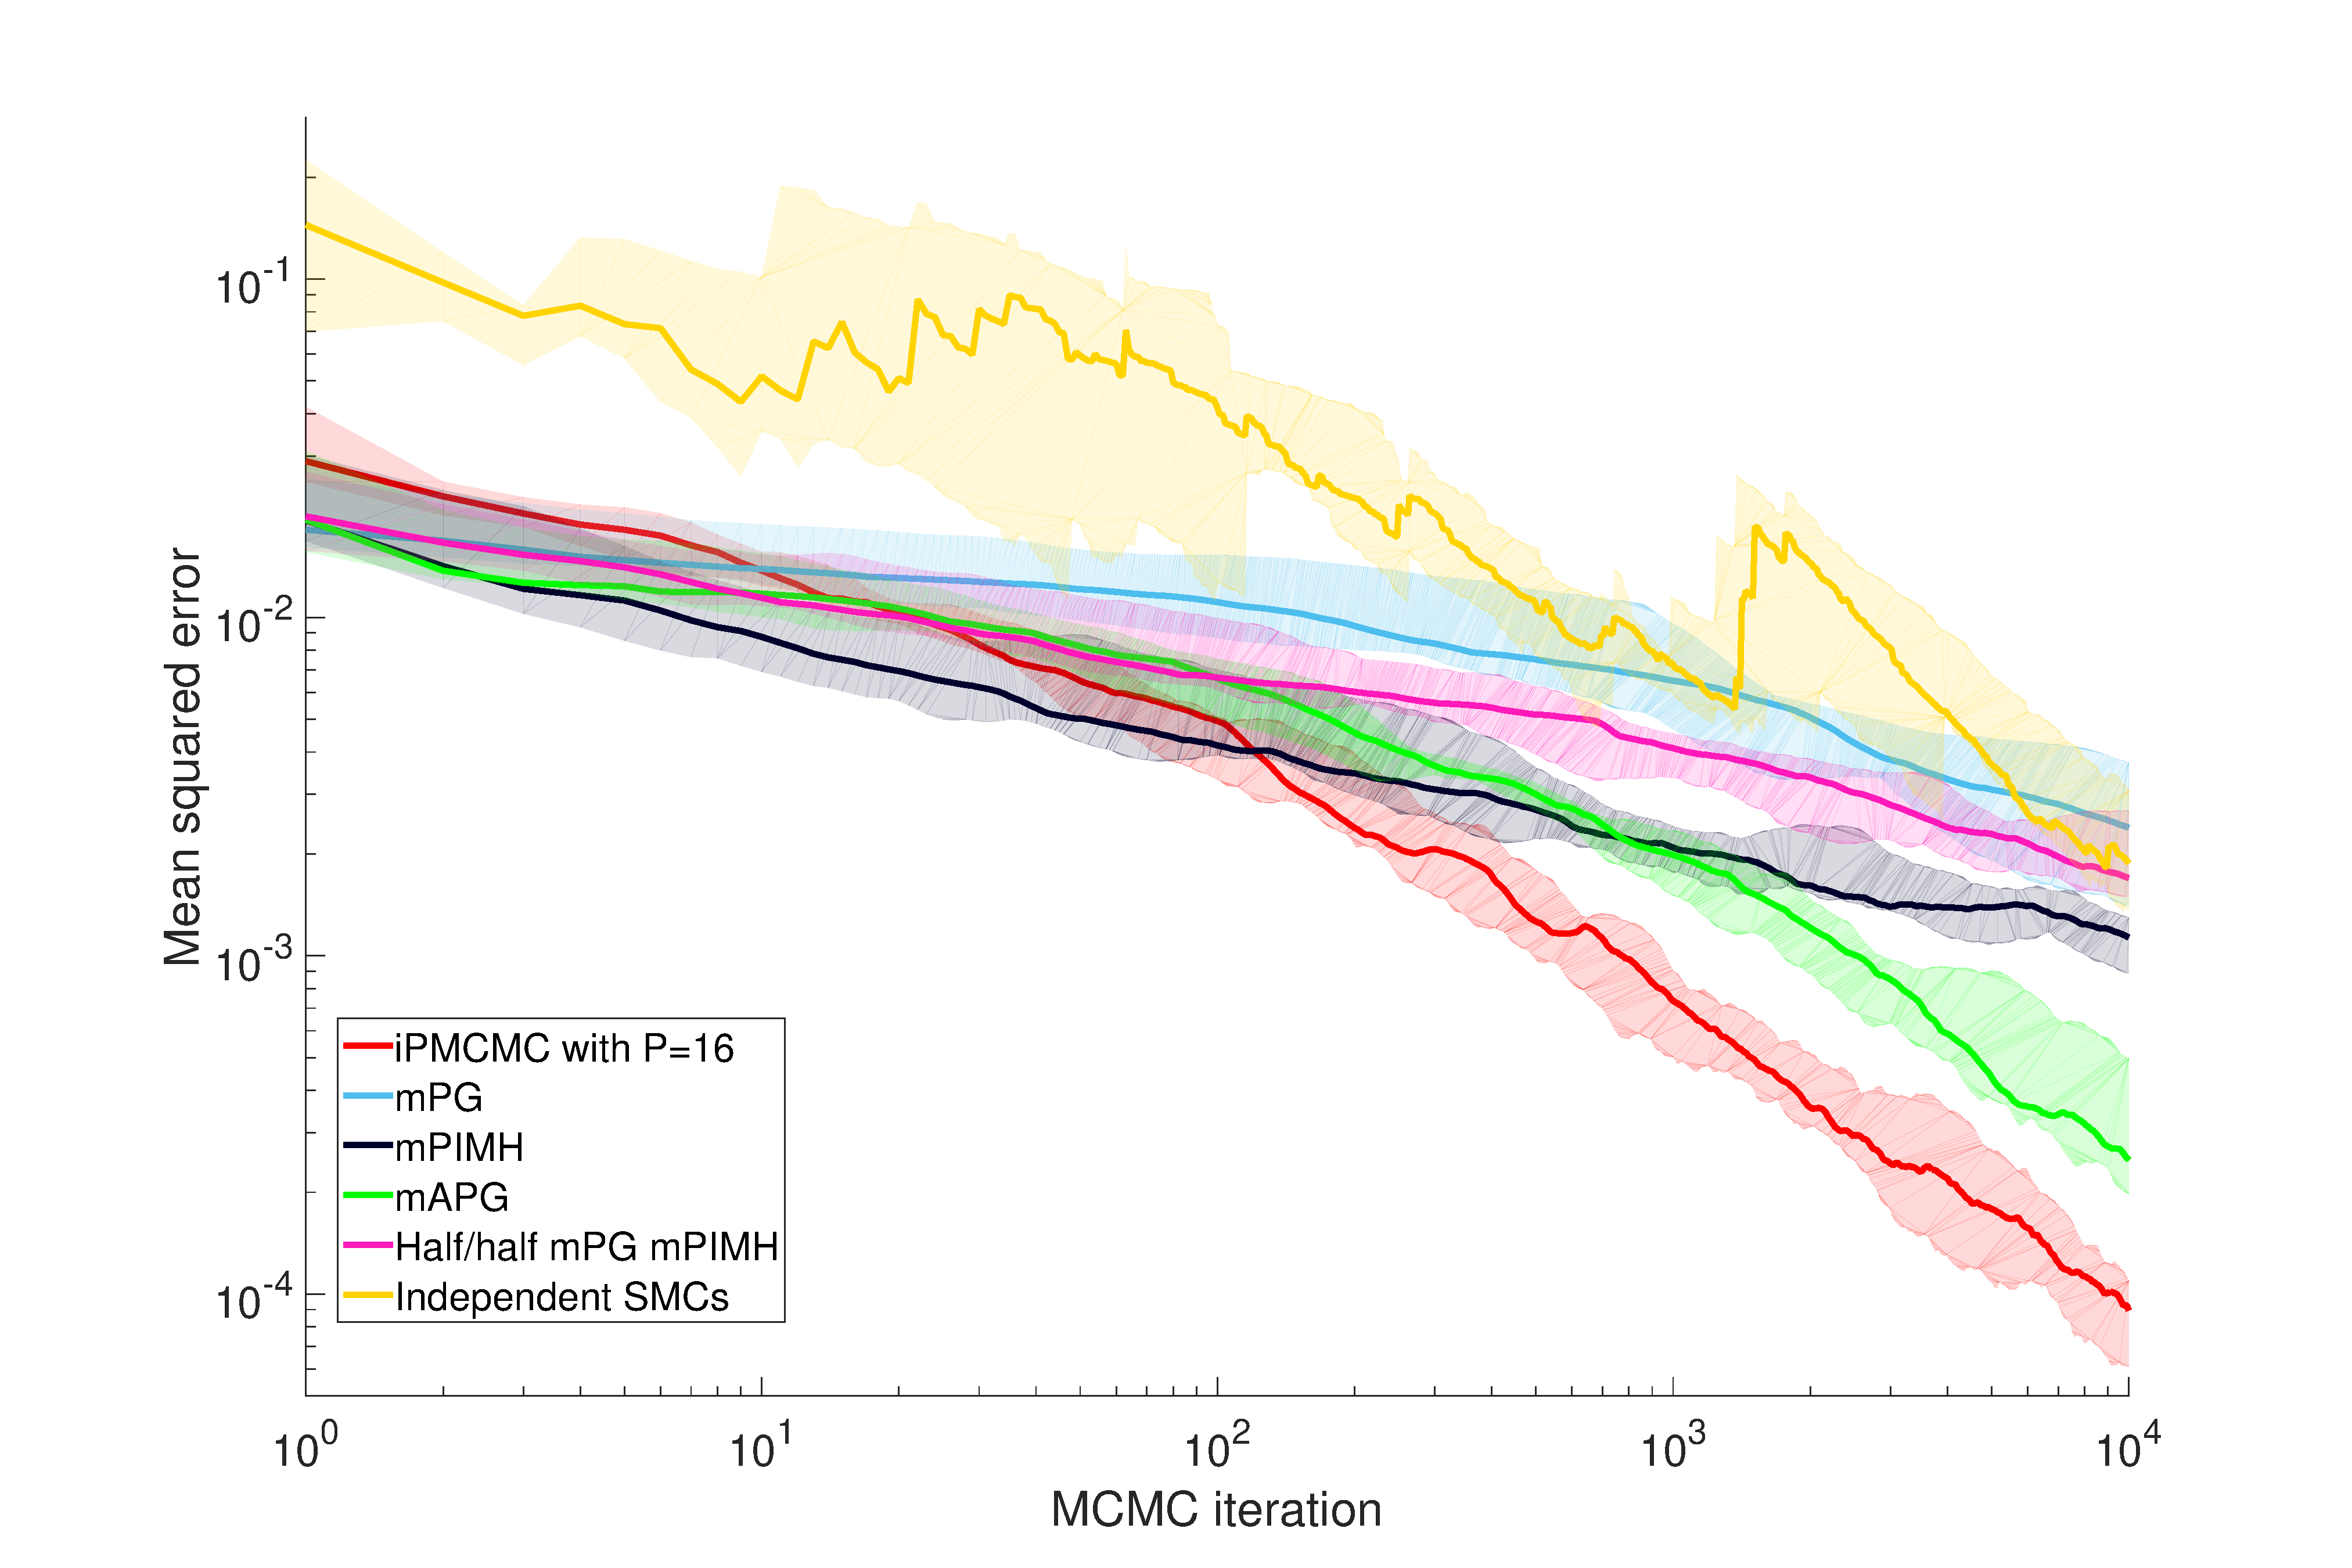
\includegraphics[width=1.1\textwidth,trim={4cm 0 5cm 0},clip]{mean_conv_distributable_lss}}
		\caption{Convergence in mean}
		\label{fig:supp-mean_dist_conv}
	\end{subfigure}
	~ %add desired spacing between images, e. g. ~, \quad, \qquad, \hfill etc. 
	%(or a blank line to force the subfigure onto a new line)
	\begin{subfigure}[t]{0.49\textwidth}
		\makebox[\textwidth][l]{\includegraphics[width=1.1\textwidth,trim={4cm 0 5cm 0},clip]{mean_pos_distributable_lss}}
		\caption{Final error in mean}
		\label{fig:supp-mean_dist_pos}
	\end{subfigure}
	
	\begin{subfigure}[t]{0.49\textwidth}
		\makebox[\textwidth][r]{\includegraphics[width=1.1\textwidth,trim={4cm 0 5cm 0},clip]{std_conv_distributable_lss}}
		\caption{Convergence in standard deviation}
		\label{fig:supp-std_dist_conv}
	\end{subfigure}
	~ %add desired spacing between images, e. g. ~, \quad, \qquad, \hfill etc. 
	%(or a blank line to force the subfigure onto a new line)
	\begin{subfigure}[t]{0.49\textwidth}
		\makebox[\textwidth][l]{\includegraphics[width=1.1\textwidth,trim={4cm 0 5cm 0},clip]{std_pos_distributable_lss}}
		\caption{Final error in standard deviation}
		\label{fig:supp-std_dist_pos}
	\end{subfigure}	
	\caption{Mean squared error in latent variable mean and standard deviation averaged over all dimensions of the LGSSM as a function of MCMC iteration (left) and position in the state sequence (right) for a selection of paraellelizable SMC and PMCMC methods.  See figure 3 in main paper for more details. \label{fig:supp-distributable_error_lss}}
\end{figure*}

\begin{figure*}[p]
	\centering
\begin{subfigure}[t]{0.49\textwidth}
	\makebox[\textwidth][r]{\includegraphics[width=1.1\textwidth,trim={4cm 0 5cm 0},clip]{skewness_conv_distributable_lss}}
	\caption{Convergence in skewness}
	\label{fig:supp-ske_dist_conv}
\end{subfigure}
~ %add desired spacing between images, e. g. ~, \quad, \qquad, \hfill etc. 
%(or a blank line to force the subfigure onto a new line)
\begin{subfigure}[t]{0.49\textwidth}
	\makebox[\textwidth][l]{\includegraphics[width=1.1\textwidth,trim={4cm 0 5cm 0},clip]{skewness_pos_distributable_lss}}
	\caption{Final error in skewness}
	\label{fig:supp-ske_dist_pos}
\end{subfigure}	

\begin{subfigure}[t]{0.49\textwidth}
	\makebox[\textwidth][r]{\includegraphics[width=1.1\textwidth,trim={4cm 0 5cm 0},clip]{kurtosis_conv_distributable_lss}}
	\caption{Convergence in kurtosis}
	\label{fig:supp-kurt_dist_conv}
\end{subfigure}
~ %add desired spacing between images, e. g. ~, \quad, \qquad, \hfill etc. 
%(or a blank line to force the subfigure onto a new line)
\begin{subfigure}[t]{0.49\textwidth}
	\makebox[\textwidth][l]{\includegraphics[width=1.1\textwidth,trim={4cm 0 5cm 0},clip]{kurtosis_pos_distributable_lss}}
	\caption{Final error in kurtosis}
	\label{fig:supp-kurt_dist_pos}
\end{subfigure}	
	\caption{Mean squared error in latent variable skewness and kurtosis averaged over all dimensions of the LGSSM as a function of MCMC iteration (left) and position in the state sequence (right) for a selection of paraellelizable SMC and PMCMC methods.  See figure 3 in main paper for more details. \label{fig:supp-distributable_error_lss2}}
\end{figure*}


\begin{figure*}[p]
	\centering
	\begin{subfigure}[t]{0.49\textwidth}
		\makebox[\textwidth][r]{\includegraphics[width=1.1\textwidth,trim={2cm 0.7cm 2cm 0},clip]{mean_conv_series_lss}}
		\caption{Convergence in mean}
		\label{fig:supp-mean_series_conv}
	\end{subfigure}
	~ %add desired spacing between images, e. g. ~, \quad, \qquad, \hfill etc. 
	%(or a blank line to force the subfigure onto a new line)
	\begin{subfigure}[t]{0.49\textwidth}
		\makebox[\textwidth][l]{\includegraphics[width=1.1\textwidth,trim={4cm 0 5cm 0},clip]{mean_pos_series_lss}}
		\caption{Final error in mean}
		\label{fig:supp-mean_series_pos}
	\end{subfigure}
	
	\begin{subfigure}[t]{0.49\textwidth}
		\makebox[\textwidth][r]{\includegraphics[width=1.1\textwidth,trim={2cm 0.7cm 2cm 0},clip]{std_conv_series_lss}}
		\caption{Convergence in standard deviation}
		\label{fig:supp-std_series_conv}
	\end{subfigure}
	~ %add desired spacing between images, e. g. ~, \quad, \qquad, \hfill etc. 
	%(or a blank line to force the subfigure onto a new line)
	\begin{subfigure}[t]{0.49\textwidth}
		\makebox[\textwidth][l]{\includegraphics[width=1.1\textwidth,trim={4cm 0 5cm 0},clip]{std_pos_series_lss}}
		\caption{Final error in standard deviation}
		\label{fig:supp-std_series_pos}
	\end{subfigure}	
	
	\caption{Mean squared error in latent variable mean and standard deviation averaged of all dimensions of the LGSSM as a function of MCMC iteration (left) and position in the state sequence (right) for iPMCMC, mPG, mPIMH and a number of serialized variants.  Key for legends: sPG = single PG chain, sPIMH = single PIMH chain, iPG = single PG chain run 32 times longer, iPIMH = single PIMH chain run 32 times longer and pPG = single PG with 32 times more particles.  For visualization purposes, the chains with extra iterations have had the number of MCMC iterations normalized by 32 so that the different methods represent equivalent total computational budget. \label{fig:supp-series_error_lss}}
\end{figure*}

\begin{figure*}[p]
	\centering
	\begin{subfigure}[t]{0.49\textwidth}
		\makebox[\textwidth][r]{\includegraphics[width=1.1\textwidth,trim={4cm 0 5cm 0},clip]{skewness_conv_series_lss}}
		\caption{Convergence in skewness}
		\label{fig:supp-ske_series_conv}
	\end{subfigure}
	~ %add desired spacing between images, e. g. ~, \quad, \qquad, \hfill etc. 
	%(or a blank line to force the subfigure onto a new line)
	\begin{subfigure}[t]{0.49\textwidth}
		\makebox[\textwidth][l]{\includegraphics[width=1.1\textwidth,trim={4cm 0 5cm 0},clip]{skewness_pos_series_lss}}
		\caption{Final error in skewness}
		\label{fig:supp-ske_series_pos}
	\end{subfigure}	
	
	\begin{subfigure}[t]{0.49\textwidth}
		\makebox[\textwidth][r]{\includegraphics[width=1.1\textwidth,trim={4cm 0 5cm 0},clip]{kurtosis_conv_series_lss}}
		\caption{Convergence in kurtosis}
		\label{fig:supp-kurt_series_conv}
	\end{subfigure}
	~ %add desired spacing between images, e. g. ~, \quad, \qquad, \hfill etc. 
	%(or a blank line to force the subfigure onto a new line)
	\begin{subfigure}[t]{0.49\textwidth}
		\makebox[\textwidth][l]{\includegraphics[width=1.1\textwidth,trim={4cm 0 5cm 0},clip]{kurtosis_pos_series_lss}}
		\caption{Final error in kurtosis}
		\label{fig:supp-kurt_series_pos}
	\end{subfigure}	
	
	
	\caption{Mean squared error in latent variable skewness and kurtosis averaged of all dimensions of the LGSSM as a function of MCMC iteration (left) and position in the state sequence (right) for iPMCMC, mPG, mPIMH and a number of serialized variants.  Key for legends: sPG = single PG chain, sPIMH = single PIMH chain, iPG = single PG chain run 32 times longer, iPIMH = single PIMH chain run 32 times longer and pPG = single PG with 32 times more particles.  For visualization purposes, the chains with extra iterations have had the number of MCMC iterations normalized by 32 so that the different methods represent equivalent total computational budget. \label{fig:supp-series_error_lss2}}
\end{figure*}

\begin{figure*}[p]
	\centering
	\begin{subfigure}[t]{0.49\textwidth}
		\makebox[\textwidth][r]{\includegraphics[width=1.1\textwidth,trim={4cm 0 5cm 0},clip]{ess_distributed_lss}}
		\caption{ESS of distributed methods for LGSSM}
		\label{fig:supp-ESS-lss-dist}
	\end{subfigure}
	~ %add desired spacing between images, e. g. ~, \quad, \qquad, \hfill etc. 
	%(or a blank line to force the subfigure onto a new line)
	\begin{subfigure}[t]{0.49\textwidth}
		\makebox[\textwidth][l]{\includegraphics[width=1.1\textwidth,trim={4cm 0 5cm 0},clip]{ess_distributed_nlss}}
		\caption{ESS of distributed methods for NLSSM}
		\label{fig:supp-ESS-nlss-dist}
	\end{subfigure}
	
	\begin{subfigure}[t]{0.49\textwidth}
		\makebox[\textwidth][r]{\includegraphics[width=1.1\textwidth,trim={4cm 0 5cm 0},clip]{ess_series_lss}}
		\caption{ESS comparison to series equivalents for LGSSM}
		\label{fig:supp-ESS-lss-series}
	\end{subfigure}
	~ %add desired spacing between images, e. g. ~, \quad, \qquad, \hfill etc. 
	%(or a blank line to force the subfigure onto a new line)
	\begin{subfigure}[t]{0.49\textwidth}
		\makebox[\textwidth][l]{\includegraphics[width=1.1\textwidth,trim={4cm 0 5cm 0},clip]{ess_series_nlss}}
		\caption{ESS comparison to series equivalents for NLSSM}
		\label{fig:supp-ESS-nlss-series}
	\end{subfigure}	
	
	\caption{Normalized effective sample size for LGSSM (left) and NLSSM (right) for a number of distributed and series models.  Key for legends: sPG = single PG chain, sPIMH = single PIMH chain, iPG = single PG chain run 32 times longer, iPIMH = single PIMH chain run 32 times longer and pPG = single PG with 32 times more particles. \label{fig:supp-ess_extras}}
\end{figure*}


\clearpage
\bibliography{refs}

\end{document} 

